\documentclass{notes}


% ********** uncomment lines 5,6,7 for a dark pdf
% \usepackage{xcolor}
% \pagecolor[rgb]{0,0,0} %black
% \color[rgb]{0.5,0.5,0.5} %grey
%*******************



\begin{document}

%CHANGE THE INFO THAT APPEARS ON THE TITLE PAGE AND THE HEADERS
\instructor{Instructor: Valentino \textsc{Tosatti}\par}
\courseid{MATH 466}
\author{Alexander Kroitor}
\version{Fall 2020}
\university{McGill University}

\begin{titlepage}
%CHANGE THE TITLE OF THE PAPER
    \title{Complex Analysis}
    \maketitle
\end{titlepage}



\setcounter{lecnum}{0}
\setcounter{page}{1}
\tableofcontents
%\thispagestyle{empty}

\begin{note}[From Scribe]
This is a set of notes for MATH466 at McGill taught by Valentino Tosatti in the Fall of 2020. For any questions, comments, corrections, requests, complaints, or insults please feel free to e-mail alexander.kroitor@mail.mcgill.ca.\\
 
 I will happily provide the most recent set of notes I have made and the source .tex files. These notes are intended to follow the lectures exactly. Some of the less compelling examples have been excluded.
\end{note}

\begin{note}[To Scribe and Interested Readers]
All lectures, especially 6 and 7, deserve a thorough review for readability. The section on Ascoli in chapter 7 is confused, and needs the insight from lecture 8 included. All lectures need to have appropriate section/subsection markers added to them, especially invisible ones for important results. The format and style change as I go and improve at latex, so earlier chapters should be revisited to standardize them.\\

I need to go back and change up the old notation to be perfectly consistent -- an example is the old $\HH = \{ x \in \C \mid \Im(x) > 0\}$ format versus the more graphically and syntactically correct $\HH = \set{ x \in \C \mid \Im(x) > 0 }$ format.\\

Note further that this \LaTeX\ code is meant to be compiled in pdfLaTeX, and will not work in other compilers (to my knowledge).
\end{note}




%FILL IN THE RIGHT INFO.
%\lecture{**LECTURE-NUMBER**}{**DATE**}
\unchapter{Lecture 1}
\lecture{1}{September 3}
\setcounter{section}{0}
\setcounter{theorem}{0}
Double REVIEWED
% **** YOUR NOTES GO HERE:

\section{Introduction to Complex Numbers}\label{sec:intro-cplx-nums}

The set of complex numbers $\mathbb{C}$ is essentially $\mathbb{R}^2$ but with extra structure, notably that $i^2=-1$. Here are some basic facts about complex numbers (with $z=a+bi$):
\begin{enumerate}
    \item $(a_1+b_1i)+(a_2+b_2i)=(a_1+a_2)+(b_1+b_2)i$
    \item $\lambda(a+bi)=\lambda a + \lambda b i$
    \item $(a_1+b_1i)(a_2+b_2i)=(a_1a_2-b_1b_2)+(a_1b_2+a_2b_1)i$
    \item $\overline{z}=a-bi$
    \item $\abs{z}=\sqrt{a^2+b^2}$
    \item $z \cdot \overline{z}=a^2+b^2= \abs{z}^2$
    \item $\overline{z_1+z_2}=\overline{z_1}+\overline{z_2}$
    \item $\overline{z_1 \cdot z_2} = \overline{z_1} \cdot \overline{z_2}$
    \item $\Re(z)=a=\frac{z+\overline{z}}{2}$
    \item $\Im(z) = b = \frac{z-\overline{z}}{2i} = -i\cdot\frac{z-\overline{z}}{2}$
    \item $\frac{1}{z} = \frac{\overline{z}}{\abs{z}^2}$ for $z \neq 0$
\end{enumerate}

Facts 1 to 3 make $\mathbb{C}$ a field with the additive identity $(0+0i)$ and the multiplicative identity $(1+0i)$. The complex conjugate (from 4) 'flips' the number across the real line. Fact 11 is implied directly by fact 6.

\subsubsection{Polar Form}

Consider $z=a+bi$. Then you can express the same z in polar form $(r,\theta)$, with $z= r e^{i\theta}$, $r\geq0$, and $\theta \in [0,2 \pi)$. To convert:
\begin{itemize}
    \item $a=r \cos \br{ \theta } , \, b=r \sin \br{\theta}$
    \item $r = \abs{z}, \, \theta = \arg(z)$
\end{itemize}

Which lead to: $z=a+bi=r \br{ \cos \br{\theta} +i \sin \br{\theta } }$. This leads to the multiplication tricks:
\begin{align*}
\text{with } & z_1=r_1 \br{ \cos \br{\theta_1 } +i \sin \br{\theta_1 } }\\
\text{and } & z_2=r_2 \br{ \cos \br{\theta_2 } +i \sin \br{\theta_2 } }
\end{align*}
\begin{itemize}
    \item $z_1\cdot z_2 = r_1 \cdot r_2 \br{ \cos \br{\theta_1+\theta_2}+i \sin\br{\theta_1+\theta_2}}$
    \item $\frac{1}{z} = \frac{1}{r} \br{ \cos \br{ -\theta } +i \sin \br{ -\theta } }$
    \item $z^n = r^n \br{ \cos\br{n\theta}+i \sin\br{n\theta}}$.
\end{itemize}


\section{Introduction to Complex Functions}

The big idea of complex analysis is to study functions that are differentiable in the complex sense. We study functions $f:\Omega \xrightarrow{} \mathbb{C}$ with $\Omega \subseteq \mathbb{C}$, $\Omega$ open and connected (called a \textbf{domain}).


\begin{definition}[Holomorphism]
$f:\Omega \xrightarrow{} \mathbb{C}$ is said to be \textbf{holomorphic} if $\forall z_0 \in \Omega$, the following limit exists:
\begin{align*}
    \lim_{h\xrightarrow{} 0} \frac{f(z_0+h)-f(z_0)}{h} =\vcentcolon f'(z_0) \in \mathbb{C}\\
\end{align*}

\end{definition}

The fact that $h\in \mathbb{C}$ is crucial; $h$ can approach $z_0$ from anywhere, and the limit must be the same and exist no matter the approach. Here is an example of a non-holomorphic function:

\begin{counterexample}\label{cex:non-hlc}
$f(z)=\Re(z)$, $\Omega = \mathbb{C}$ is not holomorphic as (letting $z = z_1 + i z_2$ and $h = h_1 + i h_2$):
\begin{align*}
    f'(z) &= \lim_{h\xrightarrow{} 0}\frac{f(z+h)-f(z)}{h}\\
    &= \lim_{h\xrightarrow{} 0}\frac{z_1+h_1-z_1}{h_1+ih_2} = \lim_{h\xrightarrow{} 0}\frac{h_1}{h_1+ih_2}\\
    \text{(if h1 = 0)} &= \lim_{h\xrightarrow{} 0}\frac{0}{ih_2}=0\\
    \text{(if h2 = 0)} &= \lim_{h\xrightarrow{} 0}\frac{h_1}{h_1}=1
\end{align*} which are not equal.
\end{counterexample}

\begin{lemma}
If $\Omega \subset \mathbb{C}$, $f,g:\Omega \xrightarrow{} \mathbb{C}$ holomorphic, then the following are holomorphic and expand in the following ways:
\begin{itemize}
    \item $f+g$; $(f+g)' = f'+g'$
    \item $f \cdot g$; $(f \cdot g)' = f' \cdot g +f \cdot g'$\\
    \item $\frac{f}{g}$; $\left( \frac{f}{g} \right)' = \frac{f'g-fg'}{g^2} \text{ for every $x_0$ such that $g(x_0) \neq 0$ }$\\
    \item if $f:\Omega\xrightarrow{}\Omega' \subset \mathbb{C}$ and $g:\Omega'\xrightarrow{}\mathbb{C}$ are hol'c\\ then $(g \circ f)$ is also hol'c and $(g \circ f)'(z) = g'(f(z))\cdot f'(z)$
\end{itemize}
\end{lemma}

\begin{proof}
The proof of these facts are identical to the real case, and as such excluded.
\end{proof}\\



We can view a complex function $f:\Omega \xrightarrow[]{} \mathbb{C}$ as a function $f:U \xrightarrow{} \mathbb{R}^2$ with $U \subset \mathbb{R}^2$. In this sense then we can write
\begin{align*}
f(z)=f(x+yi)=f(x,y) &= \Re (f(x,y)) + i \Im (f(x,y))\\ &= u(x,y)+iv(x,y)
\end{align*}

Note that $u(x,y),v(x,y) \in \mathbb{R}$, and that when added together (along with the $i$) they map from $\mathbb{R}^2$ to $\mathbb{R}^2$.

\subsection{Cauchy-Riemann Equations}

We now want to see what $f(x,y)$ being holomorphic implies for $u(x,y)$ and $v(x,y)$. The idea is to copy what was done in counterexample (\ref{cex:non-hlc}), and consider the limit from the horizontal axis and from the vertical axis.\\

For now we only consider one direction: what is implied about $u(x,y)$ and $v(x,y)$ when $f(x,y)$ is holomorphic?\\

\isubsection{THM: Cauchy-Riemann Equations}

\begin{theorem}[Cauchy-Riemann Equations]\label{thm:holc-implies-CR}
Let $f:U \xrightarrow{} \mathbb{R}^2$ holomorphic with $U \subset \mathbb{R}^2$. Let $f(x,y) = u(x,y)+iv(x,y)$. Then $\frac{\partial u}{\partial x} = \frac{\partial v}{\partial y}$ and $\frac{\partial u}{\partial y} = -\frac{\partial v}{\partial x}$.
\end{theorem}

\begin{proof}
Let $f(z)$ be holomorphic. Then:
\begin{align*}
    \lim_{h\xrightarrow{} 0} \frac{f(z+h)-f(z)}{h} \,\, \text{   exists.}
\end{align*}

Now let $h=h_1+0i$ ('horizontal' limit). This yields:
\begin{align*}
     f'(z) = \lim_{h_1\xrightarrow{} 0} \frac{f(x+h_1,y)-f(x,y)}{h_1} = \frac{\partial f}{\partial x}(z) = \frac{\partial u}{\partial x} + i \frac{\partial v}{\partial x}.
\end{align*}

%fix this -- formatted weird

Doing the same with $h=0+ih_2$ ('vertical' limit) yields:
\begin{align*}
    f'(z) = \lim_{h_2\xrightarrow{} 0} \frac{f(x,y+h_2)-f(x,y)}{ih_2} = \frac{1}{i}\frac{\partial f}{\partial y}(z) = -i\frac{\partial f}{\partial y}(z) =-i&\frac{\partial u}{\partial y} +  \frac{\partial v}{\partial y}.
\end{align*}

Since $f(z)$ is holomorphic, these two different approaches must yield equal results. Note also that two complex expressions are only equal if their real parts are equal and their complex parts are equal. This yields:
\begin{align*}
    f = u + i v \text{ holomorphic} \implies
    \begin{cases}
        \frac{\partial u}{\partial x} = \frac{\partial v}{\partial y},\\
        \frac{\partial u}{\partial y} = -\frac{\partial v}{\partial x}.
    \end{cases}
\end{align*}
And we are done.
\end{proof}\\

These are called the Cauchy-Riemann equations, and they are very important for this class and will be studied in the future. This implies that if $f(x,y)$ is holomorphic, then its components $u(x,y)$ and $v(x,y)$ must satisfy this system of 2 partial differential equations.

\begin{remark}
Recall from section (\ref{sec:intro-cplx-nums}), facts 9 and 10, that given a complex number $z=x+iy$ and its complex conjugate $\overline{z} = x-iy$, we can recover the full information about x and y using $x=\frac{z+\overline{z}}{2}$ and $y=b = \frac{z-\overline{z}}{2i}$. We can thus think of a function $f(x,y)$ as a function "$f(z,\overline{z})$". This class will not use this form.
\end{remark}


This way of writing leads to the question of the value of $f(z)$ differentiated with respect to $z$ and $\overline{z}$:
\begin{align*}
    &\frac{\partial f}{\partial z} = \frac{\partial f}{\partial x}\frac{\partial  x}{\partial z} + \frac{\partial f}{\partial y}\frac{\partial y}{\partial z} = \frac{1}{2} \frac{\partial f}{\partial x} - \frac{i}{2} \frac{\partial f}{\partial y}\\\\
    &\frac{\partial f}{\partial \overline{z}} = \frac{\partial f}{\partial x}\frac{\partial  x}{\partial \overline{z}} + \frac{\partial f}{\partial y}\frac{\partial y}{\partial \overline{z}} = \frac{1}{2} \frac{\partial f}{\partial x} + \frac{i}{2} \frac{\partial f}{\partial y}\\\\
    \text{which lead to }&\frac{\partial}{\partial z} \vcentcolon= \frac{1}{2} \left( \frac{\partial}{\partial x} - i\frac{\partial}{\partial y} \right)\\
   \text{and } &\frac{\partial}{\partial \overline{z}} \vcentcolon= \frac{1}{2} \left( \frac{\partial}{\partial x} + i\frac{\partial}{\partial y} \right)
\end{align*}

These are called the Wirtinger Derivatives. They are useful only for the following corollaries:
\isubsection{THM: Holomorphic iff CR}
\begin{corollary}\label{cor:wirt-iff-CR}
$\frac{\partial f}{\partial \overline{z}} = 0$ $\Leftrightarrow$ f(z) satisfies the Cauchy-Riemann equations.
\end{corollary}

\begin{proof} By the Wirtinger Derivatives we get:
\begin{align*}
\frac{\partial f}{\partial \overline{z}} = \frac{1}{2} \left( \frac{\partial u}{\partial x} + i\frac{\partial v}{\partial x} + i \frac{\partial u}{\partial y} - \frac{\partial v}{\partial y}\right) = 0
\end{align*}

Matching up the real and the imaginary portions leads to:
\begin{align*}
    &\frac{\partial u}{\partial x} = \frac{\partial v}{\partial y}\\
    \text{and } \, & \frac{\partial u}{\partial y} = -\frac{\partial v}{\partial x}
\end{align*}
The Cauchy-Riemann equations.
\end{proof}\\

This suggests that a function $f(z)$ is holomorphic if $\frac{\partial f}{\partial \overline{z}} = 0$, or if $f(z)$ does not depend on $\overline{z}$. An example of this in action is the fact that $f(z)=\overline{z}$ is not holomorphic.\\

In the same vein we have the following corollary:

\begin{corollary}
Assume f(z) to be holomorphic. Then $\frac{\partial f}{\partial z} = f'(z)$.
\end{corollary}

\begin{proof}
By the Wirtinger Derivatives then:
\begin{align*}
\frac{\partial f}{\partial z} &= \frac{1}{2}\left( \frac{\partial u}{\partial x} +i\frac{\partial v}{\partial x} -i\frac{\partial u}{\partial y}+\frac{\partial v}{\partial y}\right)\\
&=\frac{1}{2}\left( \frac{\partial u}{\partial x} + \frac{\partial u}{\partial x} + i\frac{\partial v}{\partial x} + i\frac{\partial v}{\partial x}\right)\\
&= \frac{\partial u}{\partial x} + i\frac{\partial v}{\partial x}\\
&= \frac{\partial f}{\partial x}\\
\text{(apply holc) } &= f'(z)
\end{align*}
And we are done.
\end{proof}\\

These two corollaries can be combined to the following theorem:

\begin{theorem}\label{thm:CR-implies-holc}
Let $f=u+iv:\Omega \xrightarrow{} \mathbb{C}$ and assume $f$ is $C^1$ (implies that u' and v' are continuous and exist). Assume that $f(z)$ satisfies the Cauchy-Riemann equations. Then $f(z)$ is holomorphic.
\end{theorem}

\begin{proof}
$u(x,y)$ and $v(x,y)$ are assumed to be continuous. This gives, using the Taylor Expansion formula:
\begin{align*}
    u(x+h_1,y+h_2) - u(x,y) &= \frac{\partial u}{\partial x}h_1 + \frac{\partial u}{\partial y}h_2 +\abs{h}\psi_1(h)\\
    v(x+h_1,y+h_2) - v(x,y) &= \frac{\partial v}{\partial x}h_1 + \frac{\partial v}{\partial y}h_2 +\abs{h}\psi_2(h)
\end{align*}
where $h=h_1+ih_2$ and $\psi_1(h),\psi_2(h) \xrightarrow[]{h \to 0} 0$.

\begin{align*}
    f(z+h)-f(z) &= u(x+h_1,y+h_2) - u(x,y) +i(v(x+h_1,y+h_2) - v(x,y))\\
    &= \frac{\partial u}{\partial x}h_1 + \frac{\partial u}{\partial y}h_2 + i\left(\frac{\partial v}{\partial x}h_1 + \frac{\partial v}{\partial y}h_2\right) + \abs{h}(\psi_1(h)+i\psi_2(h))\\
    \text{(apply CR) } &= \left( \frac{\partial u}{\partial x} -i\frac{\partial u}{\partial y}\right)(h_1+ih_2)+\abs{h}(\psi_1(h)+i\psi_2(h))\\&= \left( \frac{\partial u}{\partial x} -i\frac{\partial u}{\partial y}\right)(h)+\abs{h}(\psi_1(h)+i\psi_2(h))\\
    &\Downarrow\\
    \frac{f(z+h)-f(z)}{h}& = \left(\frac{\partial u}{\partial x} -i\frac{\partial u}{\partial y}  \right)(z) + \cancelto{0}{(\psi_1(h)+i\psi_2(h))}
\end{align*}

This implies that $f(z)$ is holomorphic.
\end{proof}

\begin{remark}
Combining theorem (\ref{thm:holc-implies-CR}) and theorem (\ref{thm:CR-implies-holc}) shows that $f$ holomorphic $\iff$ $f$ satisfies the Cauchy-Riemann equations.
\end{remark}


\begin{remark}
If you view $f(z)$ as $(u(x,y), v(x,y))$ and assume $f(z)$ is holomorphic. Computing the Jacobian matrix of (u,v) times a vector containing $h_1$ and $ih_2$ gives:
\begin{align*}
    \left( 
    \begin{matrix}
        \frac{\partial u}{\partial x} & \frac{\partial u}{\partial y} \\
        \frac{\partial v}{\partial x} & \frac{\partial v}{\partial y}
    \end{matrix}
    \right)
    \left(
    \begin{matrix}
        h_1 \\
        ih_2
    \end{matrix}
    \right)
    &= \frac{\partial u}{\partial x}h_1 +i\frac{\partial u}{\partial y} + \frac{\partial v}{\partial x}h_1 +i\frac{\partial v}{\partial y}h_2\\
    &=\frac{\partial u}{\partial x}h_1 + \frac{\partial u}{\partial y}h_2 + i\left(\frac{\partial v}{\partial x}h_1 + \frac{\partial v}{\partial y}h_2\right)\\
    &=\left(\frac{\partial u}{\partial x} -i\frac{\partial u}{\partial y}  \right)h\\
    &= f'(z)h
\end{align*}

This implies that provided $f$ is holomorphic, the action of the Jacobian on this vector is approximately the same as the mess up above.
\end{remark}

\begin{remark}
We have that:
\begin{align*}
    \left|
    \begin{matrix}
        \frac{\partial u}{\partial x} & \frac{\partial u}{\partial y} \\
        \frac{\partial v}{\partial x} & \frac{\partial v}{\partial y}
    \end{matrix}
    \right|
    &\overset{CR}{=}
    \left|
    \begin{matrix}
        \frac{\partial u}{\partial x} & \frac{\partial u}{\partial y} \\
        -\frac{\partial u}{\partial y} & \frac{\partial u}{\partial x}
    \end{matrix} \right|\\
    &= \left(\frac{\partial u}{\partial x}\right)^2 + \left(\frac{\partial u}{\partial y}\right)^2\\
    &= \abs{f'(z)}^2\geq 0
\end{align*}
since we saw earlier that $f'(z) = \left( \frac{\partial u}{\partial x} -i\frac{\partial u}{\partial y}\right)$. This shows that the determinant of the Jacobian is non-negative, and is thus orientation-preserving (as long as the determinant is not equal to $0$).
\end{remark}

%FILL IN THE RIGHT INFO.
%\lecture{**LECTURE-NUMBER**}{**DATE**}
\unchapter{Lecture 2}
\lecture{2}{September 8}
\setcounter{section}{0}
\setcounter{theorem}{0}
REVIEWED
% **** YOUR NOTES GO HERE:

\section{Complex Power Series}

\begin{definition}
Consider a sequence $\{a_n\}_{n=0}^\infty \subset \mathbb{C}$. Then the \textbf{complex series} defined by this sequence is $\sum_{n=0}^\infty a_nz^n \in \C$.
\end{definition}

\begin{proposition}
Given a power series $f(z)=\sum_{n=0}^\infty a_nz^n$ then $\exists R \in [0,\infty]$ s.t. if $\abs{z}<R$ then $f(z)$ converges absolutely (i.e. $\sum_{n=0}^\infty \abs{a_n}\abs{z}^n < \infty$), and if $\,\abs{z}>R$ then $f(z)$ diverges. Furthermore:
\begin{align*}
R=\frac{1}{\limsup\limits_{n\rightarrow \infty} \, \abs{a_n}^\frac{1}{n}}
\end{align*}
This R is called the radius of convergence of $f(z)$.
\end{proposition}

\begin{proof}
Let $L=\limsup\limits_{n\rightarrow \infty} \, \abs{a_n}^\frac{1}{n}$. Assume $0<L<\infty$. Let $R=\frac{1}{L}$.

\begin{enumerate}
    \item suppose $\abs{z}<R=\frac{1}{L}$. Since the inequality is strict $\exists \varepsilon>0$ s.t. $r\vcentcolon=(L+\varepsilon)\abs{z}<1$. By definition, $\abs{a_n}^\frac{1}{n}\leq L+\varepsilon$ for large $n$. Then:
    \begin{align*}
        \abs{a_n} \abs{z}^n &\leq \br{\br{L+\varepsilon}\abs{z}}^n = r^n\\
        &\Downarrow\\
        \sum_{n=0}^N \abs{a_n}\abs{z}^n &\leq \sum_{n=0}^N r^n \leftarrow \text{converges}
    \end{align*}
    
    \item suppose $\abs{z}>R$. Choose $\varepsilon>0$ s.t. $r\vcentcolon=(L-\varepsilon)\abs{z}>1$. By definition $\exists n_j$ s.t. $\big|a_{n_j}\big|^\frac{1}{n_j}> (L-\varepsilon) \,\,\, \forall j$. Hence: 
    
    \begin{align*}
        \big|a_{n_j}\big|\abs{z}^{n_j} &\geq ((L-\varepsilon)\abs{z})^{n_j} = r^{n_j}\\
        &\Downarrow\\
        \sum_j \big|a_{n_j}\big|\abs{z}^{n_j} &\geq \sum_j r^{n_j} \leftarrow \text{diverges}
    \end{align*}
\end{enumerate}
And we are done.
\end{proof}

\begin{theorem}
Let $f(z)= \sum_{n=0}^\infty a_n z^n$ with $R_f = R>0$. Let $D_R = D_R(0) = \set{z\in \mathbb{C} : \abs{z}<R }$. Then $f(z)$ is holomorphic on $D_R$, with $f'(z)= \sum_{n=1}^\infty na_n z^{n-1}$ and $R_{f'} = R_f$.
\end{theorem}

\begin{proof}
Let $g(z) = \sum_{n=1}^\infty na_n z^{n-1}$. Then $R_g=R_f$ since:

\begin{align*}
    \limsup\limits_{n\rightarrow \infty} \, \abs{na_n}^\frac{1}{n-1} &= \limsup\limits_{n\rightarrow \infty} \, \big( \, \abs{na_n}^\frac{1}{n}\big)^{\frac{n}{n-1}}\\
    &= \limsup\limits_{n\rightarrow \infty} \, \big( \, \cancelto{1}{\abs{n}^\frac{1}{n}}\abs{a_n}^\frac{1}{n}\big)^{\cancelto{1}{\frac{n}{n-1}}} = \limsup\limits_{n\rightarrow \infty} \, \abs{a_n}^\frac{1}{n}
\end{align*}

Given $z_0 \in D_R$ choose $r>0$ s.t. $\abs{z_0}<r<R$. Then for every $N\geq 1$ let:

\begin{align*}
    S_N(z) &= \sum_{n=0}^N a_nz^n \leftarrow \text{converges}\\
    E_N(z) &= \sum_{n=N+1}^\infty a_nz^n \leftarrow \text{converges on $D_R$}
\end{align*}
Then $f(z) = S_N(z)+E_N(z)$ on $D_R$. If $h$ is such that $\abs{z_0+h}<r$, then

\begin{align*}
    \frac{f(z_0+h)-f(z_0)}{h} - g(z_0)
    & = \frac{S_N(z_0+h)-S_N(z_0)}{h} - S_N'(z_0)&& \circled{1} \\& +S_N'(z_0)-g(z_0)&& \circled{2} \\& +\frac{E_N(z_0+h)-E_N(z_0)}{h} && \circled{3}
\end{align*}

We now show that for large $N$, these lines all go to zero.

\begin{itemize}
    

    \item[\circled{3} :]
    \begin{align*}
        \abs{\frac{E_N(z_0+h)-E_N(z_0)}{h}} &\leq \sum_{n=N+1}^\infty \abs{a_n} \underbrace{\abs{\frac{(z_0+h)^n-z_0^n}{h}}}_{a^n-b^n=(a-b)(a^{n-1}+\cdots+b^{n-1})}\\
        &= \sum_{n=N+1}^\infty \abs{a_n} \abs{\frac{(z_0+h-z_0)((z_0+h)^{n-1}+\cdots+(z_0)^{n-1}}{h}}\\
        &\leq \sum_{n=N+1}^\infty \abs{a_n} \abs{\frac{h(r^{n-1}+\cdots+r^{n-1})}{h}} = \sum_{n=N+1}^\infty \abs{a_n} \big|nr^{n-1}\big|
    \end{align*}
    this is the tail of the power series $g(z)$, but we know that $g(z)$ converges absolutely on $D_R$. Thus:
    \begin{align*}
        \abs{\frac{E_N(z_0+h)-E_N(z_0)}{h}} \leq \sum_{n=N+1}^\infty \abs{a_n} \big|nr^{n-1}\big| \xrightarrow[]{N \to \infty} 0
    \end{align*}
    
    

    \item[\circled{2} :]
    \begin{align*}
        \abs{S_N'(z_0)-g(z_0)} &=\abs{\sum_{n=1}^N na_n z_0^{n-1} -\sum_{n=1}^\infty na_n z_0^{n-1}}\\
        &= \abs{\sum_{n=N+1}^\infty na_n z_0^{n-1}}
    \end{align*}
    which goes to 0 for big N.
    
    
    \item[\circled{1} :] Note that $S_N(z)$ is holomorphic at $z=z_0$, as it is a polynomial. Thus:
    \begin{align*}
        \frac{S_N(z_0+h)-S_N(z_0)}{h} - S_N'(z_0) \rightarrow 0
    \end{align*}
    
\end{itemize}

Combining these three points, we see that for $N$ sufficiently large,
\begin{align*}
    \abs{\frac{f(z_0+h)-f(z_0)}{h} - g(z_0)} \rightarrow 0
\end{align*}
And we are done.
\end{proof}



\begin{corollary}
A power series with $R>0$ is infinitely many times complex differentiable on the disk $D_R$, and the higher derivatives are obtained by term-wise differentiation of the elements in the power series.
\end{corollary}

\begin{remark}
We can consider power series centered at some point $z_0\in\mathbb{C}$ (until now we have been considering the special case $z_0 = 0$) with the form:

\begin{align*}
    f(z)&=\sum_{n=0}^\infty a_n(z-z_0)^n\\
    \text{with } f'(z)&=\sum_{n=1}^\infty na_n(z-z_0)^{n-1}\\
    & \ \vdots
\end{align*}

This has the same radius of convergence as you would expect, but it is convergent on $D_R(z_0)=\set{z\in \mathbb{C} : \abs{z-z_0}<R }$.
\end{remark}

\begin{example}[Geometric Power Series] A standard example of a power series is:
\begin{align*}
    f(z)&=\sum_{n=0}^\infty z^n\\
    R&= 1 \\
    f(z_0)&=\sum_{n=0}^N (z_0)^n = \frac{1-z_0^{N+1}}{1-z_0} \xrightarrow{N\rightarrow\infty} \frac{1}{1-z_0}
    \end{align*}
\end{example}

\begin{example}[Exponential Power Series] A second standard power series is:
\begin{align*}
    e^z&\vcentcolon=\sum_{n=0}^\infty \frac{z^n}{n!}\\
    R&= \infty\\
\end{align*}

$e^z$ is a holomorphic function on $\mathbb{C}$. Clearly if $x\in\mathbb{R}\subset\mathbb{C}$ then $e^x$ is the usual exponential function. Note that:

\begin{align*}
    (e^z)' &= \left( \sum_{n=0}^\infty \frac{z^n}{n!} \right)'= \sum_{n=1}^\infty \frac{\cancel{n}\cdot z^{n-1}}{\cancel{n}\cdot (n-1)!}= \sum_{n=0}^\infty \frac{z^n}{n!}= e^z
\end{align*}

Further note that:

\begin{align*}
    e^{z+w} = e^z\cdot e^w
\end{align*}
\end{example}

\section{Properties of $e^z$}
We now consider some interesting aspects of the function $e^x$.
\subsection{Definition of $\cos(z)$ and $\sin(z)$}

Consider $\theta \in \mathbb{R}$. Then it is a well-known fact that:

\begin{align*}
    e^{i\theta}&=\sum_{n=0}^\infty \frac{(i\theta)^n}{n!}\\
    &= \underbrace{\left( \sum_{n=0}^\infty (-1)^n \frac{\theta^{2n}}{(2n)!}  \right)}_{\cos(\theta)} + i \cdot \underbrace{\left( \sum_{n=0}^\infty (-1)^n \frac{\theta^{2n+1}}{(2n+1)!}  \right)}_{\sin(\theta)}\\
    &= \cos(\theta)+i\sin(\theta)
\end{align*}

\begin{remark}
If $z\neq0$, let $\theta = \arg(z)$. Then $z=\abs{z}\cdot e^{i\theta}$.
\end{remark}
\begin{remark}


Consider now the function $e^{iz}, \, z\in\mathbb{C}$. Then:

\begin{align*}
    e^{iz}&=\underbrace{\left( \sum_{n=0}^\infty (-1)^n \frac{z^{2n}}{(2n)!}  \right)}_{=\vcentcolon \, \cos(z)} + i \cdot \underbrace{\left( \sum_{n=0}^\infty (-1)^n \frac{z^{2n+1}}{(2n+1)!}  \right)}_{=\vcentcolon \, \sin(z)}
\end{align*}

The functions $\cos(z)$ and $\sin(z)$ are both holomorphic functions $\forall z \in \mathbb{C}$, which gives us the complex version of Euler's formula:
\begin{equation*}
e^{iz} = \cos(z) + i\sin(z)\\
\end{equation*}
Note that:
\begin{align*}
    \cos(-z) &= \cos(z)\\
    \sin(-z) &= -\sin(z)\\
    &\Downarrow\\
    e^{-iz} &= \cos(z) - i\sin(z)\\
    &\Downarrow\\
    \cos(z) &= \frac{e^{iz}+e^{-iz}}{2}\\
    \text{and } \sin(z) &= \frac{e^{iz}-e^{-iz}}{2i}
\end{align*}
\end{remark}

\begin{definition}[Analytic Functions]
\begin{math}
\Omega \subset \mathbb{C} \text{ a domain, } f:\Omega \rightarrow \mathbb{C}
\end{math}. We say that $f$ is \textbf{analytic} (on $\om$) if $\forall z_0 \in \Omega$, $\exists r>0$ s.t. $D_r(z_0) \subset \Omega$ and $\exists \{ a_n  \}_{n=0}^\infty \subset \mathbb{C}$ s.t. $f(z) = \sum_{n=0}^\infty a_n (z-z_0)^n$ and this power series converges absolutely on $D_r(z_0)$ (i.e. $f(z)$ is analytic if locally it is equal to an absolutely convergent power series).
\end{definition}

\begin{remark}
Since power series are holomorphic, then $f(z)$ analytic on  $\Omega$ $\implies$ $f(z)$ holomorphic on $\Omega$. 
\end{remark}

\begin{theorem}
Holomorphic functions are analytic.
\end{theorem}

\begin{proof}
To be done in a following lecture.
\end{proof}

\begin{remark}
This is one way in which complex analysis veers away from real analysis. This theorem is not true in real analysis; there is a big gap between differentiable and analytic in $\mathbb{R}$, but none in $\mathbb{C}$.
\end{remark}

\section{Contour/Line Integrals}
A contour integral is an integral of a function along a curve.

\subsection{Parameterized Curves in $\mathbb{C}$}

Consider a function $\gamma:[a,b] \rightarrow \mathbb{C}$ with $[a,b] \subset \mathbb{R}$. We assume that $\gamma(t)$ is at least piece-wise smooth. We often write $\gamma(t)=z(t)$ with $t\in [a,b]$.


\begin{definition}
A function $\gamma(t)$ is called \textbf{piece-wise smooth} if $\exists a=a_0<a_1< \cdots < a_N = b$ such that $\gamma(t)$ is continuous, and that $\gamma(t)$ restricted to $[a_j,a_{j+1}]$ is differentiable with $\gamma'(t)\neq 0$ $\forall t\in [a_j,a_{j+1}]$.
\end{definition}

\begin{center}

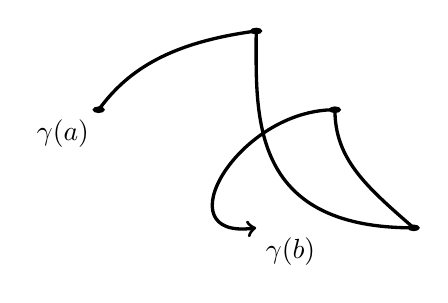
\begin{tikzpicture}[yscale=0.5]

\draw[very thick] (0,0) to [out=70,in=195] (2,2);
\draw[very thick] (2,2) to [out=270,in=180] (4,-3);
\draw[very thick] (4,-3) to [out=120,in=270] (3,0);
\draw[very thick][->](3,0) to [out=180,in=195] (2,-3);


\draw[fill] (0,0) circle [radius=2pt];
\draw[fill] (2,2) circle [radius=2pt];
\draw[fill] (4,-3) circle [radius=2pt];
\draw[fill] (3,0) circle [radius=2pt];
\node[below left] at (0,0) {$\gamma(a)$};
\node[below right] at (2,-3) {$\gamma(b)$};

\end{tikzpicture}

\textit{An example of a piece-wise smooth function.}
\end{center}


\begin{example}[CCW Circle]
Let $z(t) = z_0+e^{it}$. This traces a circle in $\mathbb{C}$.
\end{example}

\subsection{Reparameterization of Curves}

\begin{definition}
A \textbf{reparameterization} of a curve $\gamma(t)$ is a function $\Tilde{\gamma}(s) = \gamma(t(s))$ where $s\in[c,d]$ and the map  $s \mapsto t(s)$ is a smooth and strictly increasing bijection $[c,d] \rightarrow [a,b]$. The map $s \mapsto t(s)$ is called the change of parameter from the interval [c,d] to [a,b]. 
\end{definition}

\begin{note}
The mapping must be strictly increasing to ensure that the initial point of the first curve is the same as the initial point of the second curve, and the same with the end points. The curve can however be inverted:
\end{note}

\begin{example}
Consider $\gamma(b+a-t) = \Tilde{\gamma}(t)$. This reverses the direction of the curve.
\end{example}


\begin{center}

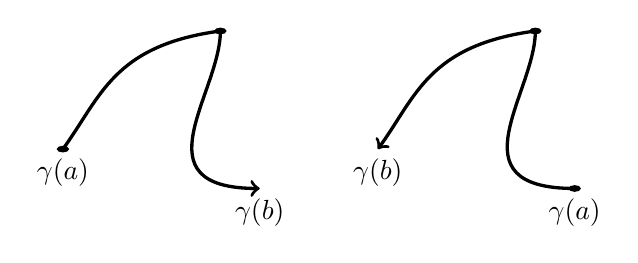
\begin{tikzpicture}[yscale=0.5]

\draw[very thick] (0,0) to [out=70,in=195] (2,3);
\draw[very thick][->] (2,3) to [out=270,in=180] (2.5,-1);
\draw[fill] (0,0) circle [radius=2pt];
\draw[fill] (2,3) circle [radius=2pt];
\node[below] at (0,0) {$\gamma(a)$};
\node[below] at (2.5,-1) {$\gamma(b)$};


\draw[very thick][<-] (4,0) to [out=70,in=195] (6,3);
\draw[very thick] (6,3) to [out=270,in=180] (6.5,-1);
\draw[fill] (6.5,-1) circle [radius=2pt];
\draw[fill] (6,3) circle [radius=2pt];
\node[below] at (6.5,-1) {$\Tilde{\gamma}(a)$};
\node[below] at (4,0) {$\Tilde{\gamma}(b)$};

\end{tikzpicture}

\textit{An example of a curve and its reversed equivalent.}
\end{center}


\begin{example}[CW circle]
Consider the parameterization $z(t) = z_0+e^{it}$ of a circle. The reparameterization $\Tilde{z}(t) = z_0+e^{-it}$ is the same circle but traced CW.
\end{example}

\subsection{Contour Integrals}
\begin{definition}[Contour Integral]
Given a parameterized (parameterized by $z(t)$) curve $\gamma(t)$ s.t. $\gamma([a,b]) \subset \Omega \subset \mathbb{C}$, and a continuous function $f:\Omega \rightarrow \mathbb{C}$, we define the \textbf{contour integral of $f(z)$ over $\gamma$} as:

\begin{align*}
    \int_{\gamma} f(z)  \dif z & \vcentcolon= \int_a^bf \br{z\br{t}} \cdot z'\br{t} \,  \dif t \in \mathbb{C}
\end{align*}

if $\gamma$ is smooth. If it is only piece-wise smooth, then:
\begin{align*}
    \int_{\gamma} f(z)  \dif z & \vcentcolon= \sum_{j=0}^{N-1} \int_{a_j}^{a_{j+1}}f\br{z\br{t}} \cdot z'\br{t} \,  \dif t \in \mathbb{C}
\end{align*}

\end{definition}


For now a contour integral is a 'black box' which takes in a parameterized curve $\gamma$ and a complex function $f(z)$ and outputs a complex number. It has some nice properties that come along with it:

\begin{itemize}
    \item The value of the integral is not dependant on the parameterization.
    \begin{align*}
        \int_{\gamma} f(z)  \dif z &= \int_a^bf(z(t)) \cdot z'(t) \,  \dif t\\
        &= \int_c^d f(z(t(s))) \cdot \underbrace{z'(t(s)) \cdot t'(s)}_{\Tilde{z}'(s) \text{ by chain rule}} \,  \dif s\\
        &= \int_c^df(\Tilde{z}(s)) \cdot \Tilde{z}'(s) \,  \dif s
    \end{align*}
\end{itemize}

More properties will come in future lectures.



%FILL IN THE RIGHT INFO.
%\lecture{**LECTURE-NUMBER**}{**DATE**}
\unchapter{Lecture 3}
\lecture{3}{September 10}
\setcounter{section}{0}
\setcounter{theorem}{0}

% **** YOUR NOTES GO HERE:

REVIEWED
\section{Complex Power Series Continued}

Recall the concept of complex power series discussed in the previous lecture: a function $f(z) = \sum_{n=0}^\infty a_nz^n$ with $a_n \in \mathbb{C}$, $z\in \mathbb{C}$. Recall that $R_f=( \limsup\limits_{n\rightarrow \infty} \, \abs{a_n}^\frac{1}{n} )^{-1}$, and that if $z<R_f, \, f(z)$ converges absolutely, and if $z>R_f$, $f(z)$ diverges.

\begin{example}[Logarithm]
\begin{align*}
    log(1+z)  `` \! \! &= \! \!"  z - \frac{z^2}{2} +\frac{z^3}{3} - \frac{z^4}{4} + \cdots\\
    &= \sum_{n=1}^\infty \frac{(-1)^{n+1}z^n}{n}\\
    R&=\frac{1}{\limsup\limits_{n\rightarrow \infty} \, \abs{a_n}^\frac{1}{n}} = \frac{1}{\limsup\limits_{n\rightarrow \infty} \, n^\frac{1}{n}} = 1.
\end{align*}

Note that the complex logarithm is more complicated than the real logarithm; it won't be a single function, but a family of functions. This power series is only one of the family. An example of the non-simplicity of the logarithm is as follows: given $0 \neq z \in \mathbb{C}$, we want $w=log(z)$ s.t. $e^w=z$. Given w we can easily find z. Given z, can we find w?
\begin{align*}
    z&=re^{i\theta}, \, r=\abs{z}>0, \, 0 \leq \theta \leq 2\pi, \, \theta = Arg(z)\\
    w&=x+iy, \, x,y\in \mathbb{R}\\\\
    e^{x+iy} &= 
    \underbrace{e^x}_{\in \mathbb{R}} \underbrace{e^{iy}}_{\in \mathbb{C}} = re^{i\theta}\\ \implies e^x &=r \implies x=log(r)\\
   \text{and } e^{iy} &= e^{i\theta} \implies y = \theta +2\pi k, \, k\in \mathbb{Z}
\end{align*}
That is to say that given $z\neq 0$, there are infinitely many w that solve $e^w=z$:
\begin{align*}
    log(z) `` \! \! = \! \! " w = log ( \,  \abs{z} )  + i\cdot (Arg(z) +2\pi k), \, k\in \mathbb{Z}
\end{align*}


which differ by adding multiples of $2 \pi i$.
\end{example}

\section{Contour Integral Properties}

We now continue some of the properties of contour integrals:

\begin{enumerate}
    \item The value of the integral is not dependant on the parameterization (as long as orientation is preserved).
    \item If $\Tilde{\gamma}$ is $\gamma$ with reverse orientation then:
    
    Let $z(t), \, a\leq t \leq b$ be a parameterization of $\gamma$. Let $\Tilde{z}(t) = z(b+a-t), \, a\leq t \leq b$ be a parameterization of $\Tilde{\gamma}$. Assume $\gamma$ is smooth (piece-wise smooth yields a similar argument on the different smooth intervals).
    \begin{align*}
         \int_{\Tilde{\gamma}} f(z)  \dif z &= \int_{a}^b f( \underbrace{z(b+a-t)}_{\Tilde{z}(t)}) \cdot (\underbrace{-z'(b+a-t)}_{\Tilde{z}'(t)})  \dif t\\
        \textit{(change variable $t \to b+a -t$)}  &= - \int_a^b f(z(t))\cdot z'(t) \dif t = - \int_{\gamma} f(z)  \dif z
    \end{align*}
    
    \item The integral operator is linear, ie $\forall \lambda, \mu \in \mathbb{C}, \, f,g$ continuous on $\mathbb{C}$:
    \begin{align*}
        \int_{\gamma} (\lambda f(z) + \mu g(z))  \dif z = \lambda \int_{\gamma} f(z)  \dif z + \mu \int_{\gamma} g(z)  \dif z
    \end{align*}
    
    \item For any $\gamma$ and $f(z)$:
    \begin{align} \label{eq:integral-bound}
    \text{with } L(\gamma) &= arclength(\gamma) = \int_a^b \abs{z'(t)}  \dif t \nonumber \\
    \abs{\int_{\gamma} f(z)  \dif z} &= \abs{\int_a^b f(z(t)) z'(t)  \dif t} \nonumber \\
    &\leq \int_a^b \abs{f(z(t))} \cdot \abs{z'(t)}  \dif t\nonumber \\
    &\leq \sup_{z \in \gamma[a,b]} \abs{f(z)} \cdot \underbrace{\int_a^b \abs{z'(t)}}_{L(\gamma)}  \dif t \nonumber \\
    &= \sup\limits_{z \in \gamma[a,b]} \abs{f(z)} \cdot L(\gamma).
    \end{align}
   
   
\end{enumerate}


\section{Complex Antiderivatives}

We now consider the complex equivalent of antiderivatives.

\begin{definition}[Antiderivatives]
Let $\Omega \subset \mathbb{C}$ open $f:\Omega \rightarrow \mathbb{C}$ holomorphic. $F:\Omega \rightarrow \mathbb{C}$ is an \textbf{antiderivative} of $f(z)$ on $\Omega$ if $F(z)$ is holomorphic and $F'(z) = f(z) \, \forall z\in\Omega $.
\end{definition}

\begin{example}
$F(z) = \frac{z^{n+1}}{n+1}$ is an antiderivative of $f(z) = z^n$ on any $\Omega \subset \mathbb{C}$.
\end{example}
\begin{example}
$f(z) = e^z$ is an antiderivative of itself.
\end{example}

\isubsection{THM: Fundamental Theorem of Calculus}
\begin{theorem}[Fundamental Theorem of Calculus \label{thm:FTC}]
Suppose that $F(z)$ is an antiderivative of $f(z)$ on some $\Omega \subset \mathbb{C}$. Let $\gamma$ be a piece-wise smooth path in $\Omega$. Then:
\begin{align*}
    \int_\gamma f(z)  \dif z &= F(\gamma(b)) - F(\gamma(a)).
\end{align*}
\end{theorem}


\begin{corollary}
If $\gamma$ is a closed curve (a curve $\gamma$ with $\gamma(a)=\gamma(b)$) then:
\begin{align*}
    \int_\gamma f(z)  \dif z &= 0.
\end{align*}

\end{corollary}

\begin{proof}[\ref{thm:FTC}]
Assume that $\gamma$ is smooth.
\begin{align*}
    \int_\gamma f(z)  \dif z &= \int_a^b f(z(t)) z'(t)  \dif t\\
    &= \int_a^b \underbrace{F'(z(t)) z'(t)}_{\frac{d}{  dt} F(z(t))}  \dif t\\
    &= \int_a^b \left( \frac{d}{ dt} F(z(t)) \right)  \dif t\\
    \text{(apply real FTC) }&= F(z(b))-F(z(a))\\
    &= F(\gamma(b)) - F(\gamma(a)).
\end{align*}

If $\gamma$ is only piece-wise smooth:
\begin{align*}
    \int_\gamma f(z) \dif z &= \sum_{j=0}^{N-1} \int_ {a_j}^{a_{j+1}} f(z(t))z'(t) \dif t\\
   \text{(apply above) } &= \sum_{j=0}^{N-1} (F(z(a_{j+1}))-F(z(a_j)))\\
   &= F(z(b)) - F(z(a)).
\end{align*}
\end{proof}

\begin{corollary}
If $f:\Omega \rightarrow \mathbb{C}$ is a holomorphic function on $\Omega$ open and connected, then $f'(z)=0 \, \forall z \in \Omega \, \implies \, f(z)$ is constant.
\end{corollary}

\begin{proof}
Since $\Omega$ is open and connected it follows (by elementary topology) that $\Omega$ is path-connected (ie given $z_0,z_1 \in \Omega \, \exists \gamma:[a,b] \rightarrow \Omega$ st $ \gamma(a) = z_0$ and $\gamma(b) = z_1$).

Apply FTC to f'(z):
\begin{align*}
    0 = \int_\gamma \underbrace{f'(z)}_{=0}  \dif z &= f(b) - f(a)\\
    \implies f(a) &= f(b)
\end{align*}
\end{proof}
\begin{remark}
Connectedness is important here, as if we don't have it we could have a function $f(z)$ defined on two sets, and constant locally on both, but not globally constant.
\end{remark}

Next week we'll continue with the proof for $f(z)$ holomorphic $\implies$ $f(z)$ analytic.

%FILL IN THE RIGHT INFO.
%\lecture{**LECTURE-NUMBER**}{**DATE**}
\unchapter{Lecture 4}
\lecture{4}{September 15}
\setcounter{section}{0}
\setcounter{theorem}{0}

% **** YOUR NOTES GO HERE:


\section{Integrals over Closed Curves}

\subsection{Goursat's Theorem}
We start by presenting the following theorem:

\isubsection{THM: Goursat's Theorem}

\begin{theorem}
Open $\Omega \subset \mathbb{C}$, $f: \Omega \rightarrow \mathbb{C}$ holomorphic. Let $T\subset \Omega$ be a (solid) triangle (this is piecewise smooth). Then:

\begin{align*}
    \int_{\partial T} f(z)  \dif z =0\\
\end{align*}

\end{theorem}


\begin{proof}
Consider a triangle T in an open set $\Omega$.




\begin{center}
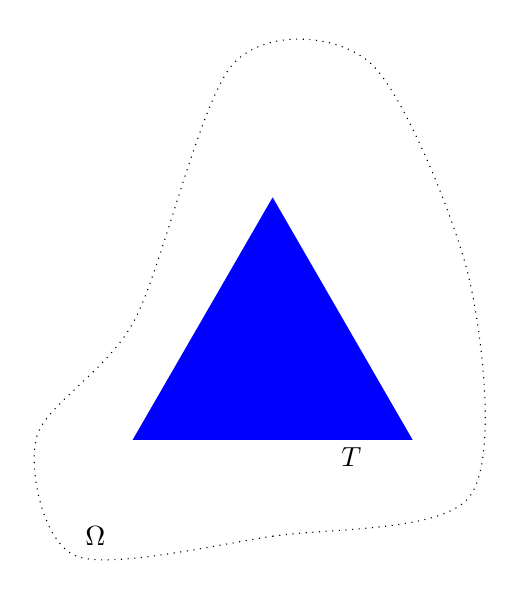
\begin{tikzpicture}
    \draw[shift={(-2.5,-2.5)},rotate=0][dotted][scale =2.5] plot [smooth cycle] coordinates {(0,0) (1,0.1) (2,0.3) (2,1.4) (1.5,2.5) (0.8,2.5) (0.3,1.2) (-0.2,0.6) };
    \draw (-2.25,-2.25) node {$\Omega$};
    
    \draw[fill=blue][scale=2] [blue,line width=1.5pt] (90:1) -- (330:1) -- (210:1) -- cycle;
    
    \draw (1,-1.25) node {$T$};
\end{tikzpicture}    
\end{center}

Subdivide T as follows: pick the midpoints of the sides, and form 4 smaller triangles by joining these points, then label these triangles $T^1,T^2,T^3,T^4$ such that $T=T^1 \cup T^2 \cup T^3 \cup T^4$:

\begin{center}
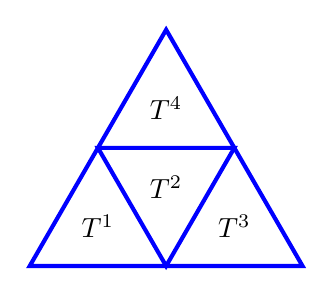
\begin{tikzpicture}
    \draw[scale=2] [blue,line width=1.5pt] (90:1) -- (330:1) -- (210:1) -- cycle;
    \draw[rotate=180][blue,line width=1.5pt] (90:1) -- (330:1) -- (210:1) -- cycle;
    \draw (0,0) node {$T^2$};
    \draw (90:1) node {$T^4$};
    \draw (90+120:1) node {$T^1$};
    \draw (90+240:1) node {$T^3$};
\end{tikzpicture}    
\end{center}

We use the positive orientation (CCW) for boundaries of triangles.


\begin{center}
%absolute cancer solution and it embarrasses me but idk how else to do this
%after some mulling maybe try applying the postaction to 1/6, 3,6 5,6 instead of 1/2 ??
\begin{tikzpicture}[very thick,decoration={
    markings,
    mark=at position 0.5 with {\arrow{<}}}
    ]
\draw[rotate =180][postaction={decorate}] [blue,line width=1.5pt] (90:1) -- (330:1) -- (210:1) -- cycle;
    \draw[rotate =60][postaction={decorate}] [blue,line width=1.5pt] (90:1) -- (330:1) -- (210:1) -- cycle;
    \draw[rotate =300][postaction={decorate}] [blue,line width=1.5pt] (90:1) -- (330:1) -- (210:1) -- cycle;
    
    \draw[shift=(90:1.5)][postaction={decorate}] [blue,line width=1.5pt] (90:1) -- (330:1) -- (210:1) -- cycle;
    \draw[rotate=120, shift=(90:1.5)][postaction={decorate}] [blue,line width=1.5pt] (90:1) -- (330:1) -- (210:1) -- cycle;
    \draw[rotate=240, shift=(90:1.5)][postaction={decorate}] [blue,line width=1.5pt] (90:1) -- (330:1) -- (210:1) -- cycle;
    
    
    \draw[shift=(210:1.5)][postaction={decorate}] [blue,line width=1.5pt] (90:1) -- (330:1) -- (210:1) -- cycle;
    \draw[rotate= 120,shift=(210:1.5)][postaction={decorate}] [blue,line width=1.5pt] (90:1) -- (330:1) -- (210:1) -- cycle;
    \draw[rotate=240,shift=(210:1.5)][postaction={decorate}] [blue,line width=1.5pt] (90:1) -- (330:1) -- (210:1) -- cycle;
    
    
    
    \draw[shift=(330:1.5)][postaction={decorate}] [blue,line width=1.5pt] (90:1) -- (330:1) -- (210:1) -- cycle;
    \draw[rotate=120, shift=(330:1.5)][postaction={decorate}] [blue,line width=1.5pt] (90:1) -- (330:1) -- (210:1) -- cycle;
    \draw[rotate= 240,shift=(330:1.5)][postaction={decorate}] [blue,line width=1.5pt] (90:1) -- (330:1) -- (210:1) -- cycle;
    
    
    \draw (0,0) node {$T^2$};
    \draw (90:1.5) node {$T^4$};
    \draw (90+120:1.5) node {$T^1$};
    \draw (90+240:1.5) node {$T^3$};
    
    
\end{tikzpicture}
\end{center}

Let $I=\int_{\partial T} f(z)  \dif z$. Observe that (since integrating over a curve backwards cancels with integrating over a curve forwards):

\begin{align*}
    I&=\int_{\partial T} f(z)  \dif z\\
    &=\sum_{n=1}^{4}\int_{\partial T^n} f(z)  \dif z
\end{align*}

Let $T_1^i = T^i$, $i=1,2,3,4$: 

\begin{center}
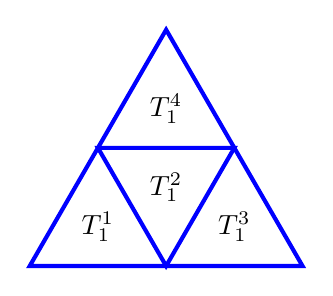
\begin{tikzpicture}
    \draw[scale=2] [blue,line width=1.5pt] (90:1) -- (330:1) -- (210:1) -- cycle;
    \draw[rotate=180][blue,line width=1.5pt] (90:1) -- (330:1) -- (210:1) -- cycle;
    \draw (0,0) node {$T^2_1$};
    \draw (90:1) node {$T^4_1$};
    \draw (90+120:1) node {$T^1_1$};
    \draw (90+240:1) node {$T^3_1$};
\end{tikzpicture}    
\end{center}

\begin{align*}
I &= \sum_{n=1}^{4}\int_{\partial T^n_i} f(z)  \dif z\\
\abs{I} &= \abs{\sum_{n=1}^{4}\int_{\partial T^n_i} f(z)  \dif z}\\
&\leq \sum_{n=1}^{4} \underbrace{\abs{\int_{\partial T^n_i} f(z)  \dif z}}_{\text{one of these is } \geq \frac{\abs{I}}{4} }\\
\end{align*}

WLOG we say that this is the first triangle:

\begin{align*}
    \abs{\int_{\partial T_1^1} f(z)  \dif z} \geq \frac{\abs{I}}{4}
\end{align*}

We then subdivide $T_1^1$ into 4 more triangles $T_2^1,T_2^2,T_2^3,T_2^4$:


\begin{center}
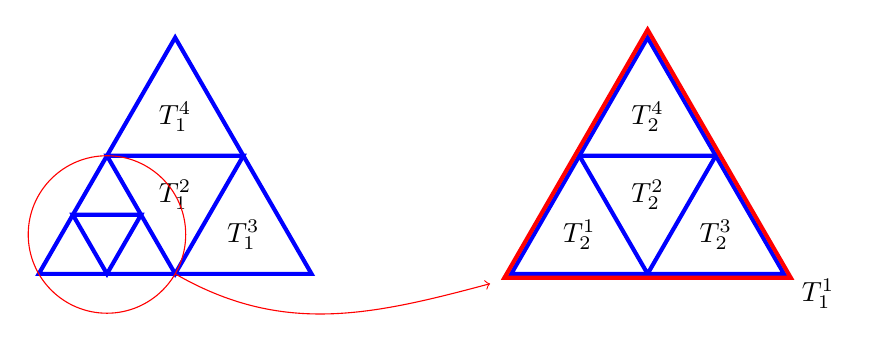
\begin{tikzpicture}

    \draw[scale=2] [blue,line width=1.5pt] (90:1) -- (330:1) -- (210:1) -- cycle;
    \draw[rotate=180][blue,line width=1.5pt] (90:1) -- (330:1) -- (210:1) -- cycle;
    \draw[scale=0.5][rotate=180, shift = (90+120:-2)][blue,line width=1.5pt] (90:1) -- (330:1) -- (210:1) -- cycle;
    \draw[shift=(0:0)] (0,0) node {$T^2_1$};
    \draw[shift=(0:0)] (90:1) node {$T^4_1$};
    \draw[shift=(0:0)] (90+240:1) node {$T^3_1$};
    \draw [color=red] (90+120: 1) circle (1);
    \draw[color = red][->] (90+120: 1)+(90+240:1) to [out=-30,in=195] (4,-1.125);


    \draw[shift=(0:6)][scale=2] [blue,line width=1.5pt] (90:1) -- (330:1) -- (210:1) -- cycle;
    \draw[shift=(0:6)][rotate=180][blue,line width=1.5pt] (90:1) -- (330:1) -- (210:1) -- cycle;
    \draw[shift=(0:6)] (0,0) node {$T^2_2$};
    \draw[shift=(0:6)] (90:1) node {$T^4_2$};
    \draw[shift=(0:6)] (90+120:1) node {$T^1_2$};
    \draw[shift=(0:6)] (90+240:1) node {$T^3_2$};
    \draw[shift=(0:6)] (90+240:2.5) node {$T^1_1$};
    \draw[shift=(0:6)][scale=2] [red,line width=1.5pt] (90:1.05) -- (330:1.05) -- (210:1.05) -- cycle;
\end{tikzpicture}    
\end{center}

We then repeat the argument just performed on the sub-triangles as well. This yields:

\begin{align*}
    \abs{\int_{\partial T_2^1} f(z)  \dif z} &\geq \frac{1}{4} \abs{\int_{\partial T_1^1} f(z)  \dif z} \geq \frac{\abs{I}}{4^2}
\end{align*}


Repeating this we get:

\begin{align}
    \abs{\int_{\partial T_k^1}f(z)  \dif z}  &\geq \frac{\abs{I}}{4^n}
\end{align}
    for the nested triangles $T \supset T_1^1 \supset T_2^1 \supset \cdots \supset T_k^1 \supset \cdots$.\\\\
We also know that:

\begin{align*}
    \text{with } diam(K) &= \sup\{ \, \abs{z-w} : z,w\in K \}\\
    diam(T_k^1) &= \frac{diam(T)}{2^k} \xrightarrow[]{\text{as } k\rightarrow \infty} 0\\
\end{align*}

Since we have a nested sequence of compact sets whose diameter shrinks to zero (means that there cannot be two points in the intersection), we have:

\begin{align*}
    \bigcap_{k=1}^\infty T_k^1 = \{ z_\infty \} \in T\\
\end{align*}



We now work near $z_\infty$. Since $f(z)$ is holomorphic:

\begin{align*}
    \lim_{z\rightarrow z_\infty} \frac{f(z) - f(z_\infty}{z-z_\infty} &\underset{exists}{=} f'(z_\infty)\\
    \implies \frac{f(z) - f(z_\infty}{z-z_\infty} &= f'(z_\infty) + \psi(z-z_\infty) \text{ (where $\psi(z-z_\infty) \rightarrow 0$)}\\
    \implies f(z) &= f(z_\infty)+f'(z_\infty)(z-z_\infty) + \psi(z-z_\infty)(z-z_\infty)\\
\end{align*}

We can try to estimate now (for k large such that $\forall z\in \partial T_k^1, \, \abs{z-z_\infty} \leq \frac{c}{2^k}$): 

\begin{align*}
    \int_{\partial T_k^1} f(z)  \dif z = \int_{\partial T_k^1} f(z_\infty)  \dif z + \int_{\partial T_k^1} f'(z_\infty)(z-z_\infty)  \dif z + \int_{\partial T_k^1} \psi(z-z_\infty)(z-z_\infty)  \dif z
\end{align*}

Now $f(z_\infty)$ is a constant holomorphic function, which thus has an antiderivative. Hence since $\partial T_k^1$ is a closed curve then by FTC:

\begin{align*}
    \int_{\partial T_k^1} f(z_\infty)  \dif z = 0
\end{align*}

Similarly:

\begin{align*}
    \int_{\partial T_k^1} f'(z_\infty)(z-z_\infty)  \dif z = 0
\end{align*}

Thus, taking the modulus of both of our remaining terms, and by applying (4.1):

\begin{align*}
    \frac{\abs{I}}{4^k} \leq \abs{\int_{\partial T_k^1} f(z)  \dif z} &= \abs{\int_{\partial T_k^1} \psi(z-z_\infty)(z-z_\infty)  \dif z}\\
    \text{(apply (3.2.4)) } &\leq \underbrace{L(\partial T_k^1)}_{=\frac{L(\partial T)}{2^k}} \underbrace{\sup\limits_{z\in \partial T_k^1}  \abs{\psi(z-z_\infty) }  }_{\leq \epsilon_k}   \underbrace{\sup\limits_{z\in \partial T_k^1} \abs{z-z_\infty}}_{\leq diam(T_k^1) = \frac{diam(T)}{2^k}} \\
    &\leq \frac{L(\partial T)}{2^k} \cdot \epsilon_k \cdot \frac{diam(T)}{2^k}\\
    &= \frac{\epsilon_k \cdot L(\partial T) \cdot diam(T) }{4^k}\\
    &\Downarrow\\
    \abs{I} & \leq \epsilon_k \cdot L(\partial T) \cdot diam(T) \xrightarrow[]{k\rightarrow \infty} 0\\
    &\Downarrow\\
    \abs{I} &= 0\\
\end{align*}

\end{proof}


\subsection{Local Existence of Antiderivatives}

\isubsection{COR: Local Existence of Antiderivatives}

\begin{corollary}[Local Existence of Antiderivatives]
Consider open $\Omega \subset \mathbb{C}$, f a holomorphic function. Then $\forall$ disks $D\subset \Omega$ $\exists F:D\rightarrow \Omega$ holomorphic $C^1$ s.t. $F'(z)=f(z) \, \forall z\in D$. That is to say that $F$ is a $C^1$ antiderivative of $f$ on $D$.
\end{corollary}

\begin{note}
$F$ a $C^1$ function $\implies$ F holomorphic and F' continuous. This must be true, since if F' is not continuous, f is not continuous and thus not holomorphic.
\end{note}



\begin{proof}
The proof uses Goursat's Theorem in a clever way. Let $D_{z_0} \subset \Omega$ be a disk centered at $z_0$. Let $L_{z_0}^z \subset D$ be the line segment from $z_0$ to $z$.

\begin{center}
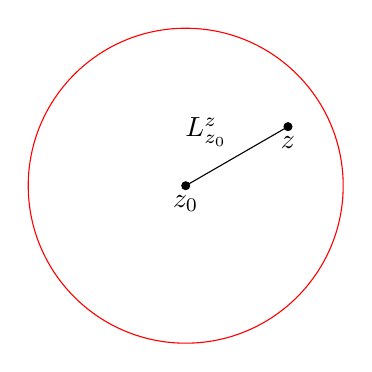
\begin{tikzpicture}[scale = 2]
    \draw [color=red] (0,0) circle (1);
    \draw[fill] (0,0) circle [radius=0.025];
    \node [below] at (0,0) {$z_0$};
    \draw[fill] (30:0.75) circle [radius=0.025];
    \node [below] at (30:0.75) {$z$};
    \draw (0,0) -- (30:0.75);
    \node [above left] at (30:0.75/2) {$L_{z_0}^z$};
\end{tikzpicture}
\end{center}

For all $z\in D$ let:

\begin{align*}
    F(z) = \int_{L_{z_0}^z} f(w) \dif w\\
\end{align*}

This defines a well-defined function $F(z)$ with $F(z_0)=0$. We now will show that $F$ is holomorphic, $C^1$, and an antiderivative of $f$.

Given $z\in D$ and $h$ small s.t. $z+h \in D$, compute:

\begin{align*}
    \frac{F(z+h)-F(z)}{h}=\frac{1}{h} \left( \int_{L_{z_0}^{z+h}} f(w) \dif w - \int_{L_{z_0}^z} f(w) \dif w \right) \\
\end{align*}

Consider the resulting triangle T inscribed in $D_{z_0}$:
\begin{center}
\begin{tikzpicture}[decoration={
    markings,
    mark=at position 0.5 with {\arrow{>}}}
    ]
    \draw [color=red] (0,0) circle (4);
    \draw[fill] (0,0) circle [radius=0.1];
    \node [below left] at (0,0) {$z_0$};
    \draw[fill] (30:3) circle [radius=0.1];
    \node [above right] at (30:3) {$z$};
    \draw[postaction={decorate}]  (0,0) -- (30:3);
    \node [above left] at (30:1.5) {$L_{z_0}^z$};
    
    \draw[postaction={decorate}] (0,0) -- (-15:2.4);
    \draw[fill] (-15:2.4) circle [radius=0.1];
    \node [below] at (-15:2.4) {$z+h$};
    \node [below] at (-15:1.2) {$L_{z_0}^{z+h}$};
    
    \draw[postaction={decorate}] (30:3) -- (-15:2.4);
    \node at (10:3.1) {$L_{z}^{z+h}$};
    \node at (10:1.5) {T};
\end{tikzpicture}
\end{center}

Then note that, by Goursat (integrating in the positive direction):

\begin{align*}
   0 \underset{Gt.}{=}\int_{\partial T} f(w)  \dif w &= \int_{L_{z_0}^{z+h}} f(w)  \dif w + \int_{L_{z+h}^{z}} f(w)  \dif w + \int_{L_{z}^{z_0}} f(w)  \dif w\\
   &= \int_{L_{z_0}^{z+h}} f(w)  \dif w - \int_{L_{z}^{z+h}} f(w)  \dif w - \int_{L_{z_0}^{z}} f(w)  \dif w\\
   &\Downarrow\\
   \frac{1}{h}\left( \int_{L_{z}^{z+h}} f(w)  \dif w \right) &=   \frac{1}{h}\left( \int_{L_{z_0}^{z+h}} f(w)  \dif w - \int_{L_{z_0}^{z}} f(w)  \dif w \right)\\
   &= \frac{F(z+h)-F(z)}{h}
\end{align*}

We then parameterize $L_{z}^{z+h}$ by $z(t) = z+t h, t\in[0,1]$ with $z'(t) = h$:

\begin{align*}
    \frac{F(z+h)-F(z)}{h} &=  \frac{1}{h}\left( \int_0^1 f(z(t)) \cdot z'(t)  \dif t \, \right)\\
    &=\frac{1}{h}\left( \int_0^1 f(z+th) \cdot h \,  \dif t \right)\\
    &= \int_0^1 f(z+th) \,  \dif t\\
    \text{($f \in C^0$; let $h\rightarrow 0$) } &= f(z)
\end{align*}

This proves that F is holomorphic, that F' = f (on D), and that F is $C^1$ (since f is continuous).

\end{proof}

Recall that by the FTC, if f is holomorphic and admits an antiderivative on an open set $\Omega$, then for any closed curve $\gamma$, $\int_\gamma f(z) \dif z = 0$

\begin{corollary}
$\Omega \subset \mathbb{C}$ open, $f:\Omega \rightarrow \mathbb{C}$ holomorphic. Then $\forall D \subset \mathbb{C}$ disc, $\forall \gamma:[a,b] \rightarrow D$ piecewise \textbf{closed} curve:

\begin{align*}
    \int_\gamma f(z) \dif z = 0\\
\end{align*}

\end{corollary}

\begin{proof}
Combine (4.2) and FTC (3.5). Then by (4.2) we find F an antiderivative for f on D. Then by FTC:
\begin{align*}
    \int_\gamma f(z) \dif z = 0\\
\end{align*}
\end{proof}

\begin{remark}
Not every holomorphic function $f:\Omega \rightarrow \mathbb{C}$ has an antiderivative on $\Omega$.

\end{remark}


\begin{example}

$\Omega = \mathbb{C}^* = \mathbb{C} \setminus \{0\}, \, f(z)=\frac{1}{z}$. This function is holomorphic on $\Omega$. 

If there were a function $F:\Omega\rightarrow\mathbb{C}$ holomorphic with $F'(z) = \frac{1}{z}$ (an antiderivative on $\mathbb{C}^*$) then with $\gamma$ being the CCW unit circle:

\begin{align*}
    \int_\gamma f(z) \dif z = 0\\
\end{align*}

But by hand (example not done in the notes) you can calculate that in fact:

\begin{align*}
    \int_\gamma f(z) \dif z = 2\pi i\\
\end{align*}

The mistake is assuming we have an antiderivative on $\mathbb{C}^*$. However by the previous theorem, if we restrict ourselves to any disc $D \subset \mathbb{C}^*$ then $\frac{1}{z}$ does have an antiderivative.

\end{example}

\begin{remark}[Uniqueness of the antiderivative]
If $f:\Omega \rightarrow \mathbb{C}$ holomorphic, and F,G are antiderivatives of f, then $F=G+c $ for some $c\in \mathbb{C}$. Thus the antiderivative is unique up to a constant.
\end{remark}

\begin{proof}
Indeed $(F-G)'= (f-f) = 0$. Thus $F-G$ is holomorphic on $\Omega$ and $F-G$ is constant.
\end{proof}

\begin{remark}[Antiderivative of $\frac{1}{z}$ on D]
Parallel to the real case, an antiderivative of $\frac{1}{z}$ is $log(z)$.
\end{remark}

This will be proved later when we have more powerful tools to work with.

\section{Multivariate Calculus Review}


We present a quick recap of multivariable calculus in $\mathbb{R}^2 = \mathbb{C}$.

Consider $\Omega \subset \mathbb{R}^2 = \mathbb{C}$ open. Consider a countable vector field $\Vec{F}$ on $\Omega$, ie a vector valued function $\Vec{F}:\Omega \rightarrow \mathbb{R}^2$. $\Vec{F}(x,y) = (P(x,y),Q(x,y))$ with $P,Q \in C^1(\overline{\Omega},\mathbb{R})$ (ie P,Q are $C^1$ functions from $\Omega$ to $\mathbb{R}^2$).

If $\gamma$ is a parameterized piecewise smooth curve in $\overline{\Omega}$ then you can define various line integrals:

\begin{align*}
    \int_\gamma P  \dif x , \int_\gamma P  \dif y,\int_\gamma Q  \dif x , \int_\gamma Q  \dif y
\end{align*}

For example if $\gamma(t) = (x(t),y(t)), t\in[a,b]$, then:

\begin{align*}
    \int_\gamma P  \dif x = \int_a^b P(x(t),y(t))\cdot x'(t) \,  \dif t\\
    \int_\gamma P  \dif y = \int_a^b P(x(t),y(t))\cdot y'(t) \,  \dif t\\
\end{align*}

\isubsection{THM: Green's Theorem}

\begin{theorem}[Green's Theorem]
Suppose $\Omega \subset \mathbb{R}^2$ is open and connected, with $\partial \Omega$ given by a piecewise smooth paramterized curve with positive (CCW) orientation. Then given $\Vec{F}(x,y) = (P(x,y),Q(x,y))$ a $C^1$ vector field as above on $\overline{\Omega}$, then:

\begin{align*}
    \int_{\partial \Omega} (P \dif x + Q \dif y) = \int_\Omega \left( \frac{\partial Q}{\partial x} - \frac{\partial P}{\partial y}  \right) \, \underbrace{ \dif A}_{ \dif x \dif y}
\end{align*}
\end{theorem}

\begin{note}
Note that these two notations are the same:

\begin{align*}
    \int_{\partial \Omega} (P \dif x + Q \dif y) &= \oint_{\partial \Omega}\Vec{F}\cdot  \dif \Vec{r}\\
    \text{and } \left( \frac{\partial Q}{\partial x} - \frac{\partial P}{\partial y}  \right) &= \triangledown \times \Vec{F} = curl(\Vec{F})
\end{align*}
\end{note}
%FILL IN THE RIGHT INFO.
%\lecture{**LECTURE-NUMBER**}{**DATE**}
\unchapter{Lecture 5}
\lecture{5}{September 17}
\setcounter{section}{0}
\setcounter{theorem}{0}

% **** YOUR NOTES GO HERE:
\section{Cauchy's Theorem}
We begin with a short discussion on what positive orientation means:
\subsection{Orientation}
Consider a blob $\Omega$ with 2 holes in it:
\begin{center}
\begin{tikzpicture}[
    tangent/.style={
        decoration={
            markings,% switch on markings
            mark=
                at position #1
                with
                {
                    \coordinate (tangent point-\pgfkeysvalueof{/pgf/decoration/mark info/sequence number}) at (0pt,0pt);
                    \coordinate (tangent unit vector-\pgfkeysvalueof{/pgf/decoration/mark info/sequence number}) at (1,0pt);
                    \coordinate (tangent orthogonal unit vector-\pgfkeysvalueof{/pgf/decoration/mark info/sequence number}) at (0pt,1);
                }
        },
        postaction=decorate
    },
    use tangent/.style={
        shift=(tangent point-#1),
        x=(tangent unit vector-#1),
        y=(tangent orthogonal unit vector-#1)
    },
    use tangent/.default=1
]

    \draw[pattern=north west lines][dotted][scale =0.5][tangent=0.25, tangent = 0.55, tangent = 0.625, tangent = 0.95]
        plot [smooth cycle] coordinates {(-10,0) (-7,3.5) (0,5)  (4,2.5) (7,0)  (5,-7) (2,-6)  (-5,-5) } (3,-1.5) circle (2) (-3,0.5) circle (3);
        
\draw [blue, thick, use tangent][->] (0.25,0) -- (-1,0);
\draw [blue, thick, use tangent][->] (0,0) -- (0,-0.5);

\draw [blue, thick, use tangent=2][->] (0.25,0) -- (-1,0);
\draw [blue, thick, use tangent=2][->] (0,0) -- (0,-0.5);

\draw [blue, thick, use tangent=3][->] (0.25,0) -- (-1,0);
\draw [blue, thick, use tangent=3][->] (0,0) -- (0,-0.5);

\draw [blue, thick, use tangent=4][->] (0.25,0) -- (-1,0);
\draw [blue, thick, use tangent=4][->] (0,0) -- (0,-0.5);

\draw node at (-3.75,-2) {$\Omega$};

\end{tikzpicture}

    
\end{center}

% \begin{center}
% \begin{tikzpicture}[
%     tangent/.style={
%         decoration={
%             markings,% switch on markings
%             mark=
%                 at position #1
%                 with
%                 {
%                     \coordinate (tangent point-\pgfkeysvalueof{/pgf/decoration/mark info/sequence number}) at (0pt,0pt);
%                     \coordinate (tangent unit vector-\pgfkeysvalueof{/pgf/decoration/mark info/sequence number}) at (1,0pt);
%                     \coordinate (tangent orthogonal unit vector-\pgfkeysvalueof{/pgf/decoration/mark info/sequence number}) at (0pt,1);
%                 }
%         },
%         postaction=decorate
%     },
%     use tangent/.style={
%         shift=(tangent point-#1),
%         x=(tangent unit vector-#1),
%         y=(tangent orthogonal unit vector-#1)
%     },
%     use tangent/.default=1
% ]

%     \draw[red][][scale =1][tangent=0.1, tangent=0.2, tangent=0.4, tangent=0.55, tangent=0.65, tangent=0.75, tangent=0.9]
%     % \draw[red][][scale =1][tangent=0.9, tangent=0.1, tangent=0.2, tangent=0.4, tangent=0.5, tangent=0.65, tangent=0.8]

%         plot [smooth cycle] coordinates {(0,1) (1,1.15) (2,0)  (1,-1.15) (0,-1) (-1,-1.15) (-2,0) (-1,1.15)};
        
% \draw [red, thick, use tangent=7][-Straight Barb] (0.01,0) -- (-0.01,0);

% \draw [thick, use tangent=1] node[cross=4pt,red] {};
% \draw [thick, use tangent=2] node[cross=4pt,red] {};

% \draw [red, thick, use tangent=3][-Straight Barb] (0.01,0) -- (-0.01,0);

% \draw [thick, use tangent=4] node[cross=4pt,red] {};
% \draw [thick, use tangent=5] node[cross=4pt,red] {};
% \draw [thick, use tangent=6] node[cross=4pt,red] {};

% % \path[use as bounding box] (-2.5,-1.5) rectangle (2.5,1.5);



% % \pattern[pattern=north east lines] (1,-1.5)--(1,1.5)--(3,1.5)--(3,-1.5)--cycle;
% % \pattern[pattern=north east lines] (-1,-1.5)--(-1,1.5)--(-3,1.5)--(-3,-1.5)--cycle;
% \pattern[pattern={mylines[size=10pt,line width=.4pt,angle=35]}] (1,-1.5)--(1,1.5)--(3,1.5)--(3,-1.5)--cycle;
% \pattern[pattern={mylines[size=10pt,line width=.4pt,angle=35]}] (-1,-1.5)--(-1,1.5)--(-3,1.5)--(-3,-1.5)--cycle;
% \draw (1,-1.5)--(1,1.5);
% \draw (-1,-1.5)--(-1,1.5);



% \end{tikzpicture}

    
% \end{center}





















If you are at a point on the curve, the positive direction is the direction such that the domain is on your left.

\subsection{Cauchy's Theorem}

\isubsection{PROP: Complex Green's Theorem}

\begin{proposition}[Complex Green's Theorem]\label{prop:green-theorem}
$\Omega \subset \mathbb{C}$ bounded open, $f:\overline{\Omega} \rightarrow \mathbb{C}, \, C^1 \, f = u+iv, \, u,v:\overline{\Omega} \rightarrow \mathbb{R}$. Assume that $\partial \Omega$ can be parameterized by piecewise smooth curves.

Then (with the parameterization in the positive direction):
\begin{align*}
    \int_{\partial \Omega} f(z)  \dif z = 2i \int_\Omega \frac{\partial f}{ \partial \overline{z}}  \dif A .
\end{align*}
This can be interpreted as a complex version of Green's Theorem.
\end{proposition}

\begin{proof}
$\Omega = \bigcup_{j=1}^n C_j$, each smooth:
\begin{align*}
    \int_{\partial \Omega} f(z)  \dif z = \sum_{j=1}^n \int_{C_j} f(z) \dif z.
\end{align*}
Parameterize each $C_j$ separately by $z(t), t\in[a,b]$. Then:
\begin{align*}
\int_{C_j} f(z)  \dif z = \int_{C_j} f(z(t))\cdot z'(t)  \dif z.
\end{align*}
Write $z(t) = (x(t),y(t)) = x(t)+iy(t)$, $z'(t) = x'(t)+iy'(t)$.
\begin{align*}
\int_{C_j} f(z)  \dif z &= \int_{C_j} f(z(t))\cdot z'(t)  \dif z\\
&= \int_a^b (u(x(t),y(t)) + iv(x(t),y(t))) \cdot (x'(t)+iy'(t))  \dif t\\
&= \int_a^b u(x(t),y(t))\cdot x'(t) \dif t - \int_a^b v(x(t),y(t)) \cdot y'(t)  \dif t \\ +&i \left[ \int_a^b u(x(t),y(t))\cdot y'(t) \dif t +  \int_a^b v(x(t),y(t))\cdot x'(t) \dif t  \right]\\
&= \int_{C_J} u \dif x - \int_{C_J} v \dif y + i \left[ \int_{C_J} u \dif y + \int_{C_J} v \dif x \right]. \\
\implies \int_{\partial \Omega} f(z)  \dif z &= \int_{\partial \Omega} (u \dif x-v \dif y) + i\int_{\partial \Omega} (u \dif y+v \dif x).
\end{align*}

Then both $\int_{\partial \Omega} (u \dif x-v \dif y)$ and $\int_{\partial \Omega} (u \dif y+v \dif x)$ are line integrals of real-valued functions. We can then apply Green's Theorem to them:
\begin{align*}
    \text{(let $\Vec{F} = (u,-v)$) }\int_{\partial \Omega} (u \dif x-v \dif y) &= \int_\Omega \left( -\frac{\partial v}{\partial x} - \frac{\partial u}{\partial y}  \right)  \dif A.\\
    \text{(let $\Vec{F} = (v,u)$) }\int_{\partial \Omega} (u \dif y+v \dif x) &= \int_\Omega \left( \frac{\partial u}{\partial x} - \frac{\partial v}{\partial y}  \right)  \dif A.\\
    \Downarrow\\
    \int_{\partial \Omega} f(z) \dif z &= i\int_\Omega \bigg(  \underbrace{\frac{\partial u}{\partial x} + i \frac{\partial v}{\partial x}}_{\frac{df}{ \dif z}} + i \bigg( \underbrace{  \frac{\partial u}{\partial y} + i \frac{\partial v}{\partial y}}_{\frac{\partial f}{\partial y}} \bigg)\bigg) \dif A\\
    &= i \int_\Omega \left( \frac{\partial f}{\partial x} + i\frac{\partial f}{\partial y} \right)  \dif A\\
   \text{(apply (\ref{cor:wirt-iff-CR}))} &= 2i \int_\Omega \frac{\partial f}{\partial \overline{z}}  \dif A.\\
\end{align*}

\end{proof}

We now get to the key result of this chapter:

\isubsection{THM: Cauchy's Theorem}
\begin{theorem}[Cauchy's Theorem]
$\Omega \subset \mathbb{C}$ open, connected, $f:\Omega \rightarrow \mathbb{C}$. Then the following are equivalent:
\begin{enumerate}
    \item f is holomorphic (in $\Omega$).
    \item $f\in C^1(\Omega)$ and $\frac{\partial f}{\partial \overline{z}} = 0$ on $\Omega$ (CR equation).
    \item $f\in C^1(\Omega)$ and $\forall \Omega' \ssubset \Omega$ (\, $\overline{\Omega'} \subset \Omega$ and compact) then $\int_{\partial \Omega'} f(z) \dif z = 0$.
    \item $f\in C^1(\Omega)$ and $\forall D = D_r(z_0) \ssubset \Omega$ and $\forall z\in D$ we have $f(z) = \frac{1}{2\pi i} \int_{\partial D} \frac{f(w)}{w-z}  \dif w$ (Cauchy's Integral Formula).
    \item $\forall D = D_r(z_0) \ssubset \Omega$ and $\forall z\in D$ we have $f(z) = \sum_{n=0}^\infty a_n (z-z_0)^n$, and this power series is absolutely convergent on D (ie $f$ is analytic on $\Omega$) and $\forall n\geq 0$, $a_n = \frac{f^{(n)}(z_0) }{n!} = \frac{1}{2\pi i} \int_{\partial D} \frac{f(w)}{(w-z)^{n+1}}  \dif w$.
\end{enumerate}
\end{theorem}





\begin{note}
Note that ($1 \leftrightarrow 2$) gained us some depth compared to before. As discussed $f$ holomorphic implies that $f$ is $C^0$, but now we know it is $C^1$ (in fact (5) implies that $f$ is $C^\infty$).

Note that (3) is a much stronger version of Goursat. Goursat is for triangles only, but this applies to many more cases (Goursat is the same statement with $\overline{\Omega'}=T$ triangle). We also proved this for disks.

Statement (4) is very important; it tells us that if you want to know the value of $f(z)$, we can find the value by computing an integral on a disk containing $z$.

Statement (5) contains a generalization of Cauchy's Integral Formula in the formula for $a_n$. Statement (4) can be recovered by letting $n=0$.
\end{note}



\begin{proof}
We will prove $(1) \Rightarrow (2) \Leftrightarrow (3) \Rightarrow (4) \Rightarrow (5) \Rightarrow (1)$.

\begin{enumerate}
    \item[$(2)\Rightarrow (3):$] This is an immediate result of theorem (\ref{prop:green-theorem}).
    \item[$(3)\Rightarrow (2):$] Suppose not, ie $\exists z_0$ s.t. $\frac{\partial f}{\partial \overline{z}} (z_0) \neq 0$. Consider $D= D_r(z_0)\ssubset \Omega$. Apply (3) to give:
    \begin{align*}
        0 = \abs{\int_{\partial D} f(z)  \dif z} \overset{Green}{=}& \abs{2i \int_D \frac{\partial f}{\partial \overline{z}}(z)  \dif A}\\
        =& 2\abs{\int_D  \left( \frac{\partial f}{\partial \overline{z}}(z) - \frac{\partial f}{\partial \overline{z}}(z_0) \right)  \dif A + \frac{\partial f}{\partial \overline{z}}(z_0) \int_D \dif A }\\
        \text{(reverse triangle ineq) } \geq&  2\abs{\frac{\partial f}{\partial \overline{z}}(z_0) \underbrace{\int_D \dif A}_{\pi r^2}}  -  2 \abs{\int_D \left( \frac{\partial f}{\partial \overline{z}}(z) - \frac{\partial f}{\partial \overline{z}}(z_0) \right)  \dif A}\\
        =& 2\pi r^2 \underbrace{\abs{\frac{\partial f}{\partial \overline{z}}(z_0)}}_{>0 \text{ assumed}} - 2 \abs{\int_D \left( \frac{\partial f}{\partial \overline{z}}(z) - \frac{\partial f}{\partial \overline{z}}(z_0) \right)  \dif A}.
    \end{align*}
    Now $f\in C^1 \implies  \frac{\partial  f }{ \partial \overline{z}} \in C^0 \implies \exists \delta>0$ s.t. if $\abs{z-z_0}< \delta$ then $\abs{ \frac{\partial f}{\partial \overline{z}}(z) - \frac{\partial f}{\partial \overline{z}}(z_0) }< \frac{1}{2}\abs{\frac{\partial f}{\partial \overline{z}}(z_0)}$. Thus:
    \begin{align*}
        2 \abs{\int_D \left( \frac{\partial f}{\partial \overline{z}}(z) - \frac{\partial f}{\partial \overline{z}}(z_0) \right)  \dif A} &\leq 2 \int_D \abs{ \frac{\partial f}{\partial \overline{z}}(z) - \frac{\partial f}{\partial \overline{z}}(z_0)}  \dif A\\
        &< \pi r^2 \abs{\frac{\partial f}{\partial \overline{z}}(z_0)}\\
        &\Downarrow\\
        0 &\geq \left( 2\pi r^2 - \pi r^2\right) \abs{\frac{\partial f}{\partial \overline{z}}(z_0)} > 0,
    \end{align*}
    which is absurd.
    \item[$(3) \Rightarrow (4):$] Assume (3). Then (2) holds. Hence $\frac{df}{d\overline{z}} = 0$ in $\Omega$. Fix $z\in\Omega$. Let $g(w) = \frac{f(w)-f(z)}{w-z}$ for $w\in\Omega \setminus \{z\}$. Then $g\in C^1(\Omega \setminus \{z\})$ and $\frac{dg}{d\overline{w}}(w) = 0$. Thus $g$ satisfies (2) and thus (3) on $\Omega \setminus \{z\}$. Apply (3) on $\Omega' = \{ \epsilon < \abs{w-z} < \delta \, | \, 0<\epsilon<\delta\}$, with $\delta$ small enough that $\Omega' \ssubset \Omega$. Then $\Omega'$ is an annulus centered at $z$:
    
    \begin{center}
    \begin{tikzpicture}[scale = 2]
    
        \draw[dotted][scale = 0.5] plot [smooth cycle] coordinates {(-3,3) (0,4) (4,3) (3,-3) (-4,-3.25) (-6,0)};
    
    
    
        \draw [color=red][pattern=north west lines][dotted][thick]  (0,0) circle (1.4);
        
        \draw [color=red][fill=white][dotted][thick] (0,0) circle (1);
        \draw[fill] (0,0) circle [radius=0.025];
        \node [below] at (0,0) {$z$};
        \draw [thick] (0,0) -- (75-90:1.4);
        \draw [thick] (0,0) -- (75-90+120:1);
        \node [below] at (75-90:0.7) {$\delta$};
        \node [left] at (75-90+120:0.5) {$\epsilon$};
        
        \node [below] at (-2,-1.35) {$\Omega$};
        \node [below] at (270+30:1.4) {$\Omega'$};
        
        
        
    \end{tikzpicture}
    \end{center}
    
    
    Applying (3) we get by (and taking the integral going clockwise on both curves):
    \begin{align*}
        0 = \int_{\partial \Omega'} g(w) \dif w &= \int_{\partial C_\delta} g(w)  \dif w - \int_{\partial C_\epsilon} g(w)  \dif w.\\
        &\Downarrow\\
        \int_{\partial C_\epsilon} g(w)  \dif w &= \int_{\partial C_\delta} g(w)  \dif w.
    \end{align*}
    
    We need a ``Taylor expansion" for $f\in C^1$.
    
    \begin{lemma}\label{lem:taylor-C1} % this might be an erroneous label, im not sure how it follows but it referenced "5.4" before which should be this
    For $f \in C^1$, $w$ sufficiently close to $z$, we have that:
    \begin{align*}
    f(w) = f(z) + \frac{\partial f}{ \partial z} (z) (w-z) + \frac{ \partial f}{ \partial \overline{z} } (z) (\overline{w}-\overline{z})+ o( \, \abs{ z-w } ).
    \end{align*}
    This is the Taylor expansion of a $C^1$ function of a complex variable. Note that $o(f)$ is a function such that $\abs{\frac{o(f)}{\abs{f}}} \rightarrow 0$.
    \end{lemma}
    \begin{proof}
    Use the real Taylor Expansion as follows:    
    \begin{align*}
        z&=x+iy\\
        w&=a+ib\\
        \text{(Taylor) } f(w) &= f(z) + \frac{\partial f }{\partial x}(z)(a-x)+ \frac{\partial f }{\partial y}(z)(b-y) +o( \, \abs{ z-w }).
    \end{align*}
    Then:
    \begin{align*}
        \frac{\partial f}{ \partial z} (z) (w-z) + \frac{ \partial f}{ \partial \overline{z} } (z) (\overline{w}-\overline{z}) &=  \frac{1}{2}\left( \frac{\partial f}{\partial x} - i\frac{\partial f}{\partial y}\right)(a+ib-x-iy)\\
        &+ \frac{1}{2}\left( \frac{\partial f}{\partial x} + i\frac{\partial f}{\partial y}\right)(a-ib-x+iy)\\
        &= \frac{\partial f }{\partial x}(z)(a-x)+ \frac{\partial f }{\partial y}(z)(b-y)
    \end{align*}
    \end{proof}
    
    Then we apply this lemma to $f$. $f$ is holomorphic so we get (after some rearranging):
    \begin{align*}
        \frac{f(w)-f(z)}{w-z} = g(w) &= \frac{\partial f}{\partial z}(z) + \frac{o( \, \abs{ z-w } ) }{w-z}\\
        \text{(let w be close to z) }&=\frac{\partial f}{\partial z}(z).
    \end{align*}
    Now g can be extended to a continuous function on all $\Omega$ (before it was defined for $w \neq z$) by letting $g(z) = \frac{\partial f}{\partial z}(z)$. Thus:
    \begin{align*}
        \abs{\int_{\partial C_\epsilon} g(w)  \dif w} &\leq L(C_\epsilon) \cdot \sup_{w\in C_\epsilon} \abs{g(w)}\\
        &= 2\pi \epsilon \cdot \underbrace{\sup_{w\in C_\epsilon} \abs{g(w)}}_{\text{bd. by (\ref{lem:taylor-C1})}}. \\
        \text{(letting $\epsilon \rightarrow 0$) } & \Downarrow\\
        0 = \int_{\partial C_\epsilon} g(w)  \dif w &= \int_{\partial C_\delta} g(w)  \dif w.
    \end{align*}
    
    Then:
    \begin{align*}
        \int_{\partial C_\delta} g(w)  \dif w &= \int_{\partial C_\delta} \frac{f(w)}{w-z}  \dif w - f(z) \underbrace{\int_{\partial C_\delta} \frac{ \dif w}{w-z}}_{compute}.
    \end{align*}
    Letting $w=z+\delta e^{it}, t\in [0,2\pi]$:
    \begin{align*}
        \int_{\partial C_\delta} \frac{ \dif w}{w-z} &= \int_{0}^{2\pi} \frac{i\delta e^{it}}{\delta e^{it}} \dif t\\
        &= i\int_{0}^{2\pi} \dif t =2 \pi i.
    \end{align*}
    Thus:
    \begin{align*}
         f(z) = \frac{1}{2\pi i}\int_{\partial C_\delta} \frac{f(w)}{w-z}  \dif w.
    \end{align*}
    
    This proves (4) when $z=z_0$. To finish the proof we assume $z_0 \neq z$.
    
    Let $D=D_\delta(z_0)$ and $D_\epsilon (z)$ with $\epsilon$ small such that $D_\epsilon (z) \subset D_\delta(z_0)$. Let $\Omega' = D_\delta(z_0) \setminus D_\epsilon (z) \ssubset \Omega$.
    
        
    \begin{center}
    \begin{tikzpicture}[scale = 2]
    
        \draw[dotted][scale = 0.5] plot [smooth cycle] coordinates {(-3,3) (0,4) (4,3) (3,-3) (-4,-3.25) (-6,0)};
    
    
    
        \draw [color=red][pattern=north west lines][dotted][thick]  (0,0) circle (1.4);
        
        \draw [color=red][fill=white][dotted][thick] (50:0.7) circle (0.4);
        \draw[fill] (50:0.7) circle [radius=0.025];
        \node [below] at (50:0.7) {$z$};
        \draw [color=white][fill=white] (270:0.125)+(75-90:0.7) circle (0.085);
        
        
        \draw [color=white][fill=white] (270:0.125) circle (0.085);
        
        \draw[fill] (0,0) circle [radius=0.025];
        
        \node at (0,-0.125) {$z_0$};
        
        \draw [thick] (0,0) -- (75-90:1.4);
        \draw [shift=(50:0.7)][thick] (0,0) -- (75-90+120:0.4);
        \node at ($ (0,-0.125)+(75-90:0.7) $) {$\delta$};
        \node [above left] at (55:0.7) {$\epsilon$};
        
        \node [below] at (-2,-1.35) {$\Omega$};
        \node [below] at (270+30:1.4) {$\Omega'$};
        
        
        
        
    \end{tikzpicture}
    \end{center}
    
    Consider the function in $w\in\Omega'$, given by$\frac{f(w)}{w-z}$. This is holomorphic and $C^1$ in $\Omega'$ (since $z \notin \Omega'$). Applying (3) gives us:
    \begin{align*}
        0 = \int_{\partial \Omega'} \frac{f(w)}{w-z}  \dif w &= \int_{\partial D_\delta (z_0)} \frac{f(w)}{w-z}  \dif w - \underbrace{\int_{\partial D_\epsilon (z)} \frac{f(w)}{w-z}  \dif w}_{=2\pi i f(z) \text{ by above}}\\
        &= \int_{\partial D_\delta (z_0)} \frac{f(w)}{w-z}  \dif w - 2\pi i f(z)\\
        &\Downarrow\\
        f(z) &= \frac{1}{2\pi i}\int_{\partial C_\delta} \frac{f(w)}{w-z} \dif w,
    \end{align*}
    Which proves it in all cases.
    
    
\item[$(4) \Rightarrow (5):$] Fix a disc $D= D_r(z_0) \ssubset \Omega$. Let $z\in D$. By (4) then:
\begin{align*}
    f(z) &= \frac{1}{2\pi i} \int_{\partial D} \frac{f(w)}{w-z}  \dif w.
\end{align*}
    
We expand $\frac{1}{w-z}$ in a power series centered at $z_0$ (so we look for a power series in $(z-z_0)$). First note that:
\begin{align*}
    \text{(since w $\in \partial D$)  } \abs{w-z_0} &= r\\
    \text{(since z $\in D \setminus \partial D$)  } \abs{z-z_0} &< r\\
    \implies \abs{\frac{z-z_0}{w-z_0}} &< 1.
\end{align*}
Thus:
\begin{align*} 
    \frac{1}{w-z} = \frac{1}{w-z_0-(z-z_0)} &= \frac{1}{w-z_0} \cdot \frac{1}{1-   \underbrace{ \left( \frac{z-z_0}{w-z_0} \right)   }_{<1}}\\
    &= \frac{1}{w-z_0} \underbrace{ \sum_{n=0}^\infty \left( \frac{z-z_0}{w-z_0} \right)^n }_{\text{absolutely convergent}}.
\end{align*}
    
Applying this to the Cauchy Integral Formula gives us:
\begin{align*}
     f(z) &= \frac{1}{2\pi i} \int_{\partial D} \left( \sum_{n=0}^\infty \left( \frac{z-z_0}{w-z_0} \right)^n \frac{f(w)}{w-z_0} \right) \dif w\\
     \text{(sum ab. conv.) } &= \sum_{n=0}^\infty \underbrace{ \left[  \frac{1}{2\pi i} \int_{\partial D}  \frac{f(w)}{(w-z_0)^{n+1}} \dif w  \right] }_{a_n} (z-z_0)^n.
\end{align*}
    
Thus $f$ is analytic and is given by the formula claimed in (5). Finally $a_n = \frac{f^{(n)} (z_0)}{n!}$. Indeed if $f(z) = \sum_{n=0}^\infty a_n (z-z_0)^n$ absolutely convergent on some disc $D \ni z$, then we proved that $f(z)$ is holomorphic and you can differentiate this power series term by term. This gives:
\begin{align*}
    &f(z) = \sum_{n=0}^\infty a_n (z-z_0)^n\\
    \implies &f(z_0) = a_0\\
    &f'(z) = \sum_{n=1}^\infty n \cdot a_n (z-z_0)^{n-1}\\
    \implies &f'(z_0) = a_1\\
    &f''(z) = \sum_{n=2}^\infty n(n-1) \cdot a_n (z-z_0)^{n-2}\\
    \implies &f''(z_0) = 2\cdot a_2\\
    &\vdots \\
    &f^{(k)}(z) = \sum_{n=k}^\infty n(n-1)\hdots(n-k+1) \cdot a_n (z-z_0)^{n-k}\\
    \implies &f^{(k)}(z_0) = k! \cdot a_k.
\end{align*}

This result holds for all convergent power series, thus it holds for this one in particular.
    
\item[$(1) \Rightarrow (2):$] Assume $f$ holomorphic on $\Omega$. $f$ satisfies the CR equations by (\ref{thm:holc-implies-CR}). We must now prove that $f \in C^1$. We use corollary (\ref{cor:local-prim}).

$\forall z \in \Omega \, \exists D = D_r(z) \ssubset \Omega$, by corollary (\ref{cor:local-prim}), $\exists F: \Omega \rightarrow \mathbb{C}$ holomorphic and $F' = f$. $F$ is holomorphic and $C^1$ (both it and its derivative are continuous) since $\frac{\partial F}{ \partial \overline{z}} =0$ and $\frac{\partial F}{ \partial z} =f(z)$ which is $C^0$ (since holomorphic functions are continuous). Thus $F$ satisfies (2) on $D$, and thus $F$ satisfies (5) and is analytic on $D$. Thus so is $f= F'$ (since the derivative of a convergent power series is also a convergent power series). Power series are $C^1$ and so we're done.
   
   
\item[$(5) \Rightarrow (1):$] This was discussed when complex power series were discussed, and is a direct application of theorem (\ref{thm:power-series-implies-CR}).
    
    
\end{enumerate}

And so we are done the proof.
\end{proof} 


\begin{note}
In statements (2), (3), and (4), $f\in C^1(\Omega)$ means that $f\in C^1(\Omega)$ in the real sense. That is to say that for $u,v$ such that $f=u+iv$ then $u,v \in C^1(\Omega)$.
\end{note}
%FILL IN THE RIGHT INFO.
%\lecture{**LECTURE-NUMBER**}{**DATE**}
\unchapter{Lecture 6}
\lecture{6}{September 22}
\setcounter{section}{0}
\setcounter{theorem}{0}

% **** YOUR NOTES GO HERE:


\section{Cauchy's Theorem Continued}

This lecture the proof of Cauchy's Theorem was continued. The rest of the proof was put with the first part of the proof in lecture 5.

We start this lecture with a corollary of Cauchy's Theorem, preceded by a rewording of a previous theorem.

\isubsection{COR: Local Existence of Alternatives version 2}

\begin{corollary}[Local Existence of Antiderivatives version 2]\label{cor:local-prim-2}
$ \oic $ open, $\foc$ continuous such that $\int_{\partial T} f(z) \dif z = 0$, $ \forall$ $T \subset \om$ triangle. Then $\forall$ disks $D\subset \Omega$ $\exists F:D\rightarrow \C$ holomorphic $C^1$ s.t. $F'(z)=f(z) \, \forall z\in D$. Thus an antiderivative of $f$ exists.
\end{corollary}

\begin{proof}
The proof for corollary (\ref{cor:local-prim}) works just as well using these assumptions.
\end{proof}

\isubsection{COR: Morera's Theorem}

\begin{corollary}[Morera's Theorem]\label{cor:morera}
$\Omega \subset \mathbb{C}$ open connected, $f:\Omega \rightarrow \mathbb{C}$ continuous such that $\int_{\partial T} f(z) \dif z = 0$, $ \forall$ T triangle. Then $f$ is holomorphic.
\end{corollary}

\begin{note}
This is the converse of theorem (\ref{thm:goursat}) (Goursat's Theorem). The proof is similar to to the proof of corollary (\ref{cor:local-prim-2}) with some slight modifications.
\end{note}






\begin{proof} Now Morera follows. Since corollary (\ref{cor:local-prim-2}) applies to $f$, we get that it has antiderivatives, so $\exists F$ s.t. $F'(z)=f(z)$. We know that $F$ is analytic, thus so is $f$. It follows that $f$ is holomorphic.

\end{proof}





We now use Cauchy's Theorem to compute some real variable integrals. Computing real integrals is one of the original motivations for exploring complex analysis and complex integrals.

\isubsection{EX: Fourier Transform}
\begin{example}[Fourier Transform of Gaussian]\label{ex:fourier-trans-gaussian}

The goal here is to compute the Fourier transform in $\R$ of the Gaussian $e^{- \pi x^2}$.  That is to say given $\xi \in \R$ we want to compute:
\begin{align*}
    \int_{-\infty}^{\infty} e^{- \pi x^2} e^{- 2 \pi i x \xi} \dif x.
\end{align*}

First let us dispense with the case where $\xi = 0$, that is to say compute:
\begin{align*}
    \int_{-\infty}^{\infty} e^{- \pi x^2} \dif x.
\end{align*}

Observe that if you square it, it becomes a double integral:
\begin{align*}
    \left(  \int_{-\infty}^{\infty} e^{- \pi x^2}  \dif x \right)^2 = \int_{\R ^2}  e^{- \pi( x^2+y^2)}  \dif A.
\end{align*}

Changing it to polar coordinates, with $\dif A = r \dif \theta \dif r $ and $x^2+y^2 = r^2$:
\begin{align*}
    \int_{\R ^2}  e^{- \pi( x^2+y^2)}  \dif A &= \int_{0}^{\infty} \int_{0}^{2 \pi} e^{- \pi r^2}  r \dif \theta \dif r \\
    &= 2 \pi \int_{0}^{\infty}  e^{- \pi r^2}  r \dif r \\
    &= -e^{-\pi r^2} \Bigr|_0^\infty = 1.
\end{align*}

Now let $\xi > 0$. Consider $f(z) =  e^{- \pi z^2}$, holomorphic on $\C$. We use Cauchy's Theorem for $f$ on a well chosen contour:

\begin{center}
\begin{tikzpicture}[very thick,decoration={
    markings,
    mark=at position 0.6 with {\arrow{>}}}
    ]
    
    \draw [thin] [->] (-4,0)--(4,0);
    \draw [thin] [->] (0,-1)--(0,3);
    
    \draw[postaction={decorate}] [blue,line width=1.5pt] (-3,0) -- (3,0);
    \draw[postaction={decorate}] [blue,line width=1.5pt] (3,2) -- (-3,2);
    \draw[postaction={decorate}] [blue,line width=1.5pt] (3,0) -- (3,2);
    \draw[postaction={decorate}] [blue,line width=1.5pt] (-3,2) -- (-3,0);
    
    
    \draw (-3,0)[below] node {$-R$};
    \draw (3,0)[below] node {$R$};
    \draw (3,2)[above] node {$R+i\xi$};
    \draw (-3,2)[above] node {$-R+i\xi$};
    
    \draw (1,0)[below] node {$\gamma_1$};
    \draw (3,1)[right] node {$\gamma_2$};
    \draw (-1,2)[above] node {$\gamma_3$};
    \draw (-3,1)[left] node {$\gamma_4$};
    
    \draw (0,1)[right] node {$\Omega_R$};
    
\end{tikzpicture}
\end{center}

$\gamma_R$ is a piecewise smooth closed curve, and $\om_R$ is the rectangle inside $\gamma_R$. $f(z)$ is holomorphic on $\C$, so in particular $f(z)$ is holomorphic on $\overline{\om_R}$. By Cauchy's Theorem then:
\begin{align*}
      0  &= \int_{\gamma_R} f(z) \dif z.\\
    \text{Thus: } 0 &= \int_{\gamma_1} e^{-\pi z^2} \dif z + \int_{\gamma_2} e^{-\pi z^2} \dif z + \int_{\gamma_3} e^{-\pi z^2} \dif z + \int_{\gamma_4} e^{-\pi z^2} \dif z.
\end{align*}

Using $z(t) = t, \, z'(t) = 1,  \, t \in [-R,R]$:
\begin{align*}
    \int_{\gamma_1} e^{-\pi z^2} \dif z = \int_{-R}^R e^{-\pi t^2}  \dif t & \xrightarrow{R\to \infty} 1.
\end{align*}

Using $z(t) = R + it, \, z'(t) = i,  \, t \in [0,\xi]$:
\begin{align*}
    \int_{\gamma_2} e^{-\pi z^2} \dif z &= \int_{0}^\xi e^{-\pi (R+it)^2} i \dif t \\ 
    &= \int_{0}^\xi e^{-\pi (R^2-t^2+2itR)} i \dif t\\
    &= i \int_{0}^\xi e^{-\pi (R^2-t^2)} e^{-2 \pi i t R}  \dif t.
\end{align*}

Then:
\begin{align*}
    \abs{\int_{\gamma_2} e^{-\pi z^2} \dif z} &= \abs{\int_{0}^\xi e^{-\pi (R^2-t^2)} e^{-2 \pi i t R}  \dif t}\\
    & \leq \int_{0}^\xi \underbrace{\abs{ e^{-\pi (R^2-t^2)} }}_{e^x > 0 \forall x \in \R} \cdot \underbrace{ \abs{e^{-2 \pi i t R} }}_{=1} \dif t\\
    &= \int_{0}^\xi e^{-\pi (R^2-t^2)}  \dif t \\ &= \int_{0}^\xi e^{-\pi R^2} e^{\pi t^2}  \dif t \\ 
    & \leq e^{-\pi R^2}  \int_{0}^\xi e^{\pi \xi^2} \dif t \\ &= e^{-\pi R^2} e^{\pi \xi^2} \xi \xrightarrow{R\to \infty} .
\end{align*}

Similarly:
\begin{align*}
    &\int_{\gamma_4} e^{-\pi z^2} \dif z \xrightarrow{R\to \infty} 0.
\end{align*}

Finally using $z(t) = i\xi +t, \, z'(t) = 1,  \, t \in [-R,R]$ (this is a reverse parameterization):
\begin{align*}
    \int_{\gamma_3} e^{-\pi z^2} \dif z &= - \int_{-R}^R e^{-\pi (t+i\xi)^2}  \dif t\\
    &= - \int_{-R}^R e^{-\pi (t+i\xi)^2}  \dif t\\
    & = - \int_{-R}^R e^{-\pi (t^2-\xi^2)} e^{-2\pi i t \xi}  \dif t\\
    &= - e^{\pi \xi ^2 } \int_{-R}^R e^{-\pi t^2} e^{-2\pi i t \xi}  \dif t.
\end{align*}

Letting $R \to \infty$, we get exactly what we wanted to evaluate in the beginning of the example. By the fact that the four integrals summed give zero we get that for $ \xi > 0$:
\begin{align*}
    - e^{\pi \xi ^2 } \int_{-\infty}^\infty &e^{-\pi t^2} e^{-2\pi i t \xi}  \dif t = -1.\\
    &\Downarrow\\
    \int_{-\infty}^\infty &e^{-\pi t^2} e^{-2\pi i t \xi}  \dif t = e^{-\pi \xi ^2 }.
\end{align*}

Similarly for $\xi < 0$ (apply a similar rectangle below the axis instead of above it):
\begin{align*}
    \int_{-\infty}^\infty e^{-\pi t^2} e^{-2\pi i t \xi}  \dif t = e^{-\pi \xi ^2 }.
\end{align*}

This implies that the Fourier transform of the Gaussian is itself.

\end{example}
\isubsection{EX: An Integral}
\begin{example}

In this example we want to compute:
\begin{align*}
    \int_0^\infty \frac{1-cos(x)}{x^2} \dif x.
\end{align*}
    
We use $f(z) = \frac{1-e^{iz}}{z^2}$, which is holomorphic on $\C \setminus \{0\}$. Then with $x\in \R$:
\begin{align*}
    \Re(f(x)) = \Re \left( \frac{1-e^{ix}}{x^2} \right) = \frac{1-cos(x)}{x^2}.
\end{align*}

Now apply Cauchy to the following contour $\gamma_{R,\epsilon}$:

\begin{center}
\begin{tikzpicture}[very thick,decoration={
    markings,
    mark=at position 0.5 with {\arrow{>}}}
    ]
    \clip (-4,-1.1) rectangle (4,4);
    %\draw (-4,-1) rectangle (4,4);
    \draw[postaction={decorate}][rotate = -120] [blue,line width=1.5pt] (0,0) circle [radius=3];
    \draw[postaction={decorate}][xscale=-1][rotate = -60] [blue,line width=1.5pt] (0,0) circle [radius=1];
    
    \draw[color=white][fill=white] (-3.5,0) rectangle (3.5,-2);
    
    
    \draw [thin] [->] (-4,0)--(4,0);
    \draw [thin] [->] (0,-1)--(0,4);
    
    \draw[postaction={decorate}] [blue,line width=1.5pt] (1-0.026,0) -- (3+0.026,0);
    \draw[postaction={decorate}] [blue,line width=1.5pt] (-3-0.026,0) -- (-1+0.026,0);
    
    %\draw[postaction={decorate}] [blue,line width=1.5pt] (-3,0) -- (3,0);
    %\draw[postaction={decorate}] [blue,line width=1.5pt] (3,2) -- (-3,2);
   % \draw[postaction={decorate}] [blue,line width=1.5pt] (3,0) -- (3,2);
    %\draw[postaction={decorate}] [blue,line width=1.5pt] (-3,2) -- (-3,0);
    
    
    \draw (-3,0)[below] node {$-R$};
    \draw (3,0)[below] node {$R$};
    \draw (-1,0)[below] node {$-\epsilon$};
    \draw (1,0)[below] node {$+\epsilon$};
    
    \draw[thick] (-0.1,0.1) -- (0.1,-0.1);
    \draw[thick] (0.1,0.1) -- (-0.1,-0.1);
    
    \draw (-2,0)[below] node {$\gamma_1$};
    \draw (2,0)[below] node {$\gamma_3$};
    \draw (120:1)[above] node {$\gamma_2$};
    \draw (120:3)[above] node {$\gamma_4$};
    
    \draw (0,1.75) [right] node {$\Omega_{R,\epsilon}$};
    
    
    
\end{tikzpicture}
\end{center}


$f$ is holomorphic on $\Omega_{R,\epsilon} \, \forall R > \epsilon >0 $. Thus Cauchy's Theorem applies and gives:
\begin{align*}
    0 = \int_{\gamma_1} f(z) \dif z +\int_{\gamma_2} f(z) \dif z +\int_{\gamma_3} f(z) \dif z +\int_{\gamma_4} f(z) \dif z .
\end{align*}

The $\gamma_1$ and $\gamma_3$ terms are useful to us since taking the real part and $\epsilon \to 0, R \to \infty$ gives us the integral we're looking for over the real line (useful to us since this function is symmetric).

Now consider the $\gamma_4$ term, $\int_{\gamma_4} f(z) \dif z $.

Consider $z=x+iy, \, y>0 $. Then $\abs{e^{iz}} = \abs{e^{ix}} \abs{ e^{-y}} = \abs{ e^{-y}} \leq 1 $ (does not apply if $z$ is in the lower half-plane). Then:
\begin{align*}
    \abs{f(z)} &= \frac{\abs{1-e^{iz}}}{\abs{z}^2}\\
    & \leq \frac{1+\abs{e^{iz}}}{\abs{z}^2} \leq \frac{2}{\abs{z}^2}.
\end{align*}

Now since $\gamma_4$ is contained in the upper half-plane:
\begin{align*}
   \abs{ \int_{\gamma_4} f(z) \dif z } &\leq L(\gamma_4) \sup_{z\in \gamma_4} \abs{f(z)}\\
   &\leq \pi R \cdot \frac{2}{R^2} \xrightarrow[]{R\to \infty} 0.
\end{align*}


Now consider the $\gamma_2$ term, $\int_{\gamma_2} f(z) \dif z $. Paramaterize $\gamma_2$ (backwards) by $z(t) = \epsilon e^{it}, t\in [0,\pi]$. Now:
\begin{align*}
    e^{iz} &= 1 + iz + \frac{(iz)^2}{2} + \frac{(iz)^3}{3!} + \hdots\\
   1- e^{iz}  &=  -iz - \frac{(iz)^2}{2} - \frac{(iz)^3}{3!} - \hdots\\
   &\Downarrow\\
   \frac{ 1- e^{iz}}{ z^2} &= - \frac{i}{z} - \frac{(iz)^2}{2z^2} - \frac{(iz)^3}{3!z^2} - \hdots\\
   &= - \frac{i}{z} + g(z),\\
   \text{with } \abs{g(z)} &\leq C \text{ for some C as } z \to 0.
\end{align*}

Note that, since $\sup_{z\in \gamma_2} (g(z))$ is bounded:
\begin{align*}
    \abs{\int_0^\pi g(z) \cdot i \epsilon e^{it} \dif t} \leq \sup_{z\in \gamma_2} (g(z)) \cdot \epsilon \pi \xrightarrow[]{\epsilon \to 0} 0.
\end{align*}


And thus:
\begin{align*}
    \int_{\gamma_2} \underbrace{\frac{ 1- e^{iz}}{ z^2}}_{f(z)} \dif z &= - \int_0^{\pi} f(\epsilon e^{it} ) \cdot i \epsilon e^{it} \dif t\\
    &= + \int_0^{\pi} \frac{i}{ \epsilon e^{it}} i \epsilon e^{it} \dif t - \int_0^\pi g(z) \cdot i \epsilon e^{it} \dif t\\
   \text{(letting $\epsilon \to 0$) } &= -\pi.
\end{align*}

Thus finally, noting that $\int_{\gamma_1} f(z) \dif z + \int_{\gamma_3} f(z) \dif z = \int_\R \frac{ 1- e^{ix}}{ x^2} \dif x$:
\begin{align*}
    0 &= \sum_{i=1}^4 \int_{\gamma_i} f(z) \dif z \\
    \text{($\epsilon \to 0$, $R \to \infty$) }&= \int_\R \frac{ 1- e^{ix}}{ x^2} \dif x - \pi. \\
   &\Downarrow\\
    \Im \left( \int_\R \frac{ 1- e^{ix}}{ x^2} \dif x \right) &=  0.\\
    \Re \left( \int_\R \frac{ 1- e^{ix}}{ x^2} \dif x \right) &=  \pi = \int_{-\infty}^{\infty} \frac{ 1- cos(x)}{ x^2} \dif x.\\
    &\Downarrow \text{ even function}\\
    \int_0^{\infty} \frac{ 1- cos(x)}{ x^2} \dif x &= \frac{\pi}{2}.\\
\end{align*}

And we are done.

\end{example}





%FILL IN THE RIGHT INFO.
%\lecture{**LECTURE-NUMBER**}{**DATE**}
\unchapter{Lecture 7}
\lecture{7}{September 24}
\setcounter{section}{0}
\setcounter{theorem}{0}

% **** YOUR NOTES GO HERE:

We start with a method for bounding the derivatives of a holomorphic function.

\section{Cauchy's Estimates}

double reviewed

\isubsection{THM: Cauchy's Estimates}

\begin{theorem}[Cauchy's Estimates]\label{thm:cauchy-estimates}

$\foc$ holomorphic function on $\oic$. Let $z_0 \in \om, r>0 $ s.t. $D=D_r(z_0) \ssubset \om$. Then $\forall n\geq 0$:  
\begin{align*}
    \abs{f^{(n)}}(z_0) \leq \frac{n!}{r^n} \cdot \sup_{\partial D}\abs{f}
\end{align*}

\end{theorem}


\begin{note}
This is linked closely to the coefficients of the power series representation of $f$. If $r$ is small (usually this is the case) then it gives you an upper bound for the growth of the derivatives, and thus for the coefficients. If $r$ is large then then these coefficients will decay.
\end{note}


\begin{proof}
This is a straightforward application of equation (\ref{eq:cauchy-int-fla}). Parameterize $D$ by $z(t) = z_0 +re^{it}$:
\begin{align*}
    \abs{f^{(n)}} &= \abs{\frac{n!}{2\pi i} \int_{\partial D} \frac{f(z)}{(z-z_0)^{n+1}} \dif z }\\
    &\leq \frac{n!}{2\pi} \abs{\int_{0}^{2\pi} \frac{f(z_0 +re^{it})}{(z_0 +re^{it}-z_0)^{n+1}} \cdot i r e^{it} \dif t }\\
    &\leq \frac{n!}{2\pi} \abs{\int_{0}^{2\pi} \frac{f(z_0 +re^{it})}{r^{n+1}e^{i(n+1)t}} \cdot r e^{it} \dif t }\\
    &\leq  \frac{n!}{2\pi} \abs{\int_{0}^{2\pi} \frac{f(z_0 +re^{it})}{r^{n}e^{int}} \dif t }\\
    &\leq \frac{n!}{2\pi} \int_{0}^{2\pi}  \frac{\abs{ f(z_0 +re^{it})  }}{r^{n}} \dif t \\
    &\leq \frac{n!}{2\pi} \sup_{\partial D}\abs{f} \int_{0}^{2\pi}  \frac{1}{r^{n}} \dif t  = \frac{n!}{r^n} \sup_{\partial D}\abs{f}.
\end{align*}
\end{proof}

\begin{note}
This theorem is the same as putting a bound on $a_n$, with $\abs{a_n} \leq \frac{\sup_{\partial D}\abs{f}}{r^n}$.
\end{note}


\begin{definition}[Entire Functions]
A function $f:\C \to \C$, f holomorphic on $\C$, is called an \textbf{entire} holomorphic function.
\end{definition}

\isubsection{COR: Liouville}

\begin{corollary}[Liouville]\label{cor:liouville}

Consider $f:\C \to \C$ entire holomorphic with $\sup_{z\in \C}\abs{f(z)} \leq C$ for some $C$. Then $f$ is constant.

More generally, $f:\C \to \C$ entire holomorphic with $\abs{f(z)} \leq C\abs{z}^k$ for some $C, k$ and for all $z \in \C$. Then $f$ is a polynomial in $z$ with degree $d\leq k$.

\end{corollary}


\begin{note}
This corollary says that if $f$ entire holomorphic grows slower than a polynomial, it is a polynomial. This implies that if $f$ entire holomorphic is not a polynomial, it must grow faster than any polynomial. Some examples are $e^z$, $\cos(z)$, and $\sin(z)$ (unlike the real case where $\cos(z)$ and $\sin(z)$ are bounded).
\end{note}

\begin{proof}
Since $f$ entire holomorphic, we know that it can be written as a power series that converges everywhere:
\begin{align*}
    f(z) = \sum_{n=1}^\infty a_n z^n \text{ (this converges for all $z\in \C$)}.
\end{align*}

We have an estimate for the growth of this $a_n$; applying theorem (\ref{thm:cauchy-estimates}) on $D_r(0)$ for any $r>0$ gives:
\begin{align*}
    \abs{a_n} = \frac{\abs{f^{(n)} (0)  }}{n!} &\leq \frac{\sup_{\partial D_r(0)}\abs{f}}{r^n}\\
    &\leq \frac{Cr^k}{r^n}.
\end{align*}

If $n>k$ this implies that $\abs{a_n} \xrightarrow[]{r\to \infty} 0$. Thus: $f(z) = \sum_{n=1}^{k} a_n z^n$ and $f$ is a polynomial of degree at most $k$.

\end{proof}

\begin{corollary}[Fundamental Theorem of Algebra]
Given any polynomial $P(z) = \sum_{n=1}^{d} a_n z^n$ of degree $d> 0$, $a_n \in \C $, $a_d \neq 0$. Then $\exists z_0 \in \C$ s.t. $P(z_0) = 0$ (it has a root).
\end{corollary}

\begin{note}
This is equivalent to saying that $\C$ is an algebraically closed field. This is false for $\R$.
\end{note}


\begin{proof}
Suppose that $P$ has no roots. Then the reciprocal is defined. $\frac{1}{P(z)}$ is an entire holomorphic function. We want to bound $\abs{\frac{1}{P(z)}} = \frac{1}{\abs{P(z)}}$. Then $P(z) = z^d( a_d + \frac{a_{d-1}}{z} + \cdots + \frac{a_0}{z^d})$. For $\abs{z} \gg 1$, we can examine $\frac{P(z)}{z^d} = ( a_d + \frac{a_{d-1}}{z} + \cdots + \frac{a_0}{z^d}) \xrightarrow[]{\abs{z}\to \infty} a_d$. That is to say that $\exists R > 0 $ s.t. $\forall \abs{z} > R$ we have:
\begin{align*}
    \abs{\frac{P(z)}{z^d}} &= \frac{\abs{P(z)}}{\abs{z^d}} > \frac{\abs{a_d}}{2}>0.\\
    &\Downarrow\\
    \frac{1}{\abs{P(z)}} &\leq \frac{2}{\abs{a_d}} \cdot \frac{1}{\abs{z}^d} \leq C \: \forall \abs{z} > R.
\end{align*}
    
Then outside the disk $D_R(0)$ $f$ is bounded. $f$ is bounded inside the disk since $\frac{1}{P(z)}$ is holomorphic, thus continuous on $D_R(0)$, and thus bounded inside the compact disk. Thus on $\C$:
\begin{align*}
     \abs{\frac{1}{P(z)}} \leq C.
\end{align*}

By corollary (\ref{cor:liouville}), $\frac{1}{P(z)} $ is a constant. Thus $P(z)$ is a constant. This is a contradiction since we assumed that $P(z) $ had positive degree.
\end{proof} 

\begin{note}
By repeating this argument we can show that $P(z)$ of degree d has exactly d roots in $\C$, possibly non-distinct. That is to say that $P(z) = a_d (z-z_1)\cdots (z-z_d)$.
\end{note}


\isubsection{THM: Zeroes are Isolated}
\begin{theorem}[Zeroes of Holomorphic Functions]\label{thm:isolated-zeroes}

$\foc$ holomorphic, $\om$ open and connected, $f \not\equiv 0$ on $\om$. Then the zeroes for $f$ inside $\om$ are isolated. That is to say that if $f(z_0)=0, \, z_0 \in \om$ then $\exists $V $\subset \om$ open such that $f(z) \neq 0 \, \forall z\in V \setminus \{0\}$.

\end{theorem}

\begin{proof}
Suppose $z_0$ is a non-isolated zero of $f$. We claim that $f\equiv 0$ in some neighbourhood of $z_0$. To show the claim, we let $f(z) = \sum_{n=1}^{\infty} a_n (z-z_0)^n$, which is absolutely convergent near $z_0$. Then if the claim is false, $\exists n >0$ s.t. $a_n\neq 0$. Define $g(z) = a_n+a_{n+1}(z-z_0) + \cdots $. Then:
\begin{align*}
    f(z) &= (z-z_0)^n(a_n+a_{n+1}(z-z_0) + \cdots )\\
    &= (z-z_0)^ng(z).
\end{align*}
$g(z)$ is the power series for $f$, but with coefficients shifted by $n$. Thus $g(z)$ is holomorphic on some small disk centered at $z_0$ (an absolutely convergent power series with shifted coefficients is still absolutely convergent on the same disk). $g(z_0) = a_n \neq 0 \xRightarrow[]{cont} g(z) \neq 0$ for $z$ close to $z_0$. Since $f(z) = (z-z_0)^ng(z)$ we get that $z_0$ cannot be a non-isolated zero of $f$.

We return to the theorem. Let $\om ' = \set{ z \in \om | f \equiv 0 \text{ in some neighbourhood of } z }$. The claim shows that $z_0 \in \om '$, and thus $\om ' \neq \varnothing$. $\om '$ is open (since for any point, $f$ is zero around that point). $\om '$ is also closed.

To see this, suppose you have a sequence $\{ z_n \}_{n=0}^\infty \in \om ', z_n \xrightarrow[]{n\to \infty} z_\infty \in \om $. $f(z_n) = 0 \xRightarrow[]{cont} f(z_\infty) = 0$. Then $z_\infty$ is a non-isolated zero of $f$ (because it is a limit of zeroes). By the claim $f \equiv 0 $ around $z_\infty$, thus $z_\infty \in \om '$. Thus $\om '$ is closed. This implies, applying connectedness, that $\om ' = \om$. Thus $f \equiv 0$ on $\om$, contradiction.

\end{proof} 


\begin{definition}[Order of Vanishing]\label{def:order-vanish}
In the proof we showed that if $f$ holomorphic in $\om \ni z_0, \: f \not\equiv 0$, then we can write $f(z) = (z-z_0)^N g(z)$, where $g \neq 0$ near $z_0$. Then N is called the \textbf{order of vanishing} of $f$ at $z_0$.



\end{definition}

\isubsection{COR: Identity Principle}

\begin{corollary}[Identity Principle]\label{cor:ident-princ}
Suppose you have $f,g: \om \to \C$ holomorphic such that $\exists \{ z_j \}_{j=0}^\infty, \, z_j \xrightarrow[]{j \to \infty} z_\infty \in \om$ (with $z_i \neq z_j$ for $i \neq j$) such that $f(z_j) = g(z_j) \, \forall j$. Then $f \equiv g$ on $\om$.
\end{corollary}

\begin{proof}
If $f-g \not\equiv 0$ then the zeroes of $f-g$ must be isolated, but they are not by the assumption (the assumption says to assume that $f-g$ has a non-isolated zero).
\end{proof}

\begin{definition}[Analytic Continuation]
Suppose you have $\om_1 \subset \om_2 $ open connected. Suppose $f: \om_1 \to \C$ holomorphic and $F: \om_2 \to \C$ holomorphic such that $f = F |_{\om_1}$ (ie $f(z) = F(z) \, \forall z \in \om_1$) then $F$ is called an \textbf{analytic continuation} of $f$ to $\om_2$.

\end{definition}


\begin{note}[Uniqueness of Analytic Continuations]

Corollary (\ref{cor:ident-princ}) shows that if $F$ and $F'$ are both analytic continuations of $f$ to $\om_2$, then $F \equiv F'$ (since $F$ and $F'$ will agree on $\om_1$ and thus are equal).

We can thus refer to $F$ as the (unique) analytic continuation of $f$ to $\om_2$.
\end{note}

We now present a bit of review material in preparation for a discussion of normal families.

\subsection{Ascoli-Arzelà's Theorem}

\begin{proposition}
Suppose that $\exists \foc$ such that $f_n \to f$ uniformly on compact subsets of $\om$. Then $f$ is holomorphic on $\om$.
\end{proposition}


\begin{proof}
Uniform convergence on compact subsets means that for any $K \subset \om$ compact then $\sup_{z\in K} \abs{f_n(z) - f(z)} \xrightarrow[]{n \to \infty} 0$. 

Using theorem (\ref{thm:goursat}) and corollary (\ref{cor:morera}), let $z\in \om$. It suffices to show that $f$ is holomorphic on $D=D_r(z) \ssubset \om $ for some $r>0$. We check that $f$ is holomorphic on $D$. Let $T \subset D$ a triangle. Then by theorem (\ref{thm:goursat}) $\int_{\partial T} f_n(z) \dif z =  0$. On the other hand, for $D \subset K \subset \om$ compact, then if $f_n \tou f$ it is easy to see that $\int_{\partial T} f_n(z) \dif z \tou \int_{\partial T} f(z) \dif z$. Thus $\int_{\partial T} f(z) \dif z = 0$.
\end{proof}

\begin{note}
This proposition says that if $f$ is a uniform limit of holomorphic functions, then $f$ is also holomorphic. This is quite bizarre; a uniform limit of smooth functions on a compact set need not be smooth. Stone-Weierstrass says that every continuous function can be uniformly approximated by polynomials (both smooth and analytic), and thus that every continuous function is a uniform limit. This is quite different compared to the complex case.
\end{note}



\begin{theorem}[Ascoli-Arzelà]\label{thm:ascoli-arzela}
Let $\om$ open. Let $\{f_n \}_{n=0}^\infty, \, f_n : \om \to \C$ holomorphic on $\om$. Suppose that
\begin{itemize}
    \item $f_n$ is uniformly bounded (ie $\sup_{z\in \om} \abs{f_n(z)} < C$ for some $C$),
    \item $\set{ f_n }$ are uniformly equicontinuous on $\om$ (ie $\forall \epsilon \exists \delta$ s.t. if $\abs{x-y} < \delta, \, x,y \in \om$, then $\abs{f_n(x) - f_n(y)} < \epsilon$ for all n).
\end{itemize}

Then $\exists \foc$ continuous (and holomorphic by the previous proposition) such that $f_{n_j} \tou f$ for some subsequence $n_j$ on compact subsets of $\om$.

\end{theorem}
 
\begin{note}\label{note:after-ascoli-arzela}
Usually Ascoli-Arzelà is assumed on $K$ compact, which results in the uniform convergence on $K$. This is an extension of the usual form. If you have the assumptions on all of $\om$, then in particular you have them for all compact subsets. Thus for every compact set you obtain a uniform limit, and by exhaustion you can see that the limit will always have to be the same function.

Ascoli-Arzelà tells you that on a compact set you have a uniform limit, which is therefore continuous, and the previous proposition tells you that this limit is holomorphic.
\end{note}
%FILL IN THE RIGHT INFO.
%\lecture{**LECTURE-NUMBER**}{**DATE**}
\unchapter{Lecture 8}
\lecture{8}{September 29}
\setcounter{section}{0}
\setcounter{theorem}{0}

% **** YOUR NOTES GO HERE:

We begin with a small remark, inspired by a previous homework set.

\begin{remark}
Let $\gamma_1, \gamma_2$ be parameterized piecewise smooth curves, with the same initial points and end points, and such that they do not cross except at endpoints (they enclose a region $\Omega$). If $f$ holomorphic on $\overline{\Omega}$ then $\int_{\gamma_1}f(z) \dif z = \int_{\gamma_2} f(z) \dif z$. This follows easily by theorem (\ref{thm:cauchy-theorem}) (Cauchy's Theorem), since $0 = \int_{\partial \Omega} = \int_{\gamma_1} - \int_{\gamma_2}$.

\begin{center}
\begin{tikzpicture}[very thick,decoration={
    markings,
    mark=at position 0.5 with {\arrow{>}}}
    ]

\draw[fill] (-3,-1) circle [radius=2pt];
\draw[fill] (3,1) circle [radius=2pt];

\draw plot [smooth, tension=2] coordinates { (-3,-1) (-2,2) (0,1.5) (1,2) (3,1)};
\draw plot [smooth, tension=2] coordinates { (-3,-1) (-1,-1) (0,1) (3,0) (3,1)};


\draw (-0.1,1.5-0.1) -- (0,1.5) -- (0-0.1,1.5+0.1);
\draw (0-0.9*0.14,1+0.4*0.14) -- (0,1) -- (0-0.4*0.14,1-0.9*0.14);

\draw (0,1.5)[above] node {$\gamma_1$};
\draw (0,1)[below] node {$\gamma_2$};
\draw (-1.5,0) node {$\om$};

\end{tikzpicture}
\end{center}


This does not hold if $f$ is not holomorphic on $\overline{\Omega}$. Consider $f(z)= \frac{1}{z}$. Then we have calculated (in an excluded example) that with $\gamma_1$ the upper half unit circle and $\gamma_2$ the lower half unit circle that $\int_{\partial D_1(0)} f(z) \dif z = - \int_{\gamma_1} f(z) \dif z + \int_{\gamma_2} f(z) \dif z = 2\pi i \neq 0$.
\end{remark}




\begin{center}
\begin{tikzpicture}[very thick,decoration={
    markings,
    mark=at position 0.5 with {\arrow{>}}}
    ]
    \draw[postaction={decorate}][xscale=1][rotate = 90] (0,0) circle [radius=1];
    \draw[postaction={decorate}][xscale=-1][rotate = -90] (0,0) circle [radius=1];
    
    \draw[fill] (-1,0) circle [radius=2pt];
    \draw[fill] (1,0) circle [radius=2pt];
    
    \draw (0,1)[below] node {$\gamma_1$};
    \draw (0,-1)[above] node {$\gamma_2$};
    \draw (-1,0)[right] node {$\om$};
    \draw[thick] (-0.1,0.1) -- (0.1,-0.1);
    \draw[thick] (0.1,0.1) -- (-0.1,-0.1);
    
\end{tikzpicture}
\end{center}





We now look at a comparatively non-trivial theorem. Montel's Theorem give us a sufficient an necessary condition for a family of holomorphic functions on a domain to converge uniformly on compact sets to some limit.


\section{Montel's Theorem}

\isubsection{THM: Montel's Theorem}
\begin{theorem}[Montel's Theorem]\label{thm:montel}
Let $f_n: \om \to \C$ holomorphic functions, $n \in \mathbb{N}$. Suppose that they are uniformly bounded on compact subsets of $\om$ (ie $\forall K \ssubset \om $ compact $ \exists C_K > 0 $ s.t. $ \sup_{z \in K} \abs{f_n(z)} \leq C_K \, \forall n)$. Then $\exists $ subsequence $n_j \to \infty, \, \exists \foc  $ holomorphic s.t. $f_{n_j} \tou f$ on compact subsets  of $\om$ and $f_{n_j}^{(k)} \tou f^{(k)}$ on compact subsets of $\om , \, \forall k \geq 0$.
\end{theorem}


\begin{definition}[Normal Family]
A set of functions is called a \textbf{normal family} if $\exists $ subsequence $n_j \to \infty$ and $ \exists \foc  $ holomorphic s.t. $f_{n_j} \xrightarrow[]{u} f$ on compact subsets of $\om$ and $f_{n_j}^{(k)} \xrightarrow[]{u} f^{(k)}$ on compact subsets of $\om , \, \forall k \geq 0$.\\

Note that the case where $k=0$ is simply the first sentence, and that if the $k=0$ case holds the $k>0$ case is implied. Thus, it is sufficient to ignore the $k>0$ case when writing the definition.
\end{definition}


\begin{remark}
Theorem (\ref{thm:montel}) states that for a set of functions, uniformly bounded on compact subsets implies normal.

If $f_n \tou f$ holomorphic on compact subsets then $f_n$ is uniformly bounded on compact subsets. Without the subsequence part, being a normal family is essentially equivalent to being uniformly bounded on compact sets.
\end{remark}


\begin{remark}
$\{ f_n \}$ uniformly bounded on compact subsets of $\om$ $\iff$ $\{ f_n \}$ locally uniformly bounded (ie $\forall \, z_0 \in \om, \, \exists \, r,C > 0 $ s.t. $ D_r(z_0) \ssubset \om$ and $\sup_{z \in D_r(z_0)} \abs{f_n(z)} \leq C$).

The right direction is simple, as each disk is covered by a compact set that is still in $\om$. To see the left direction, cover a compact set with disks. By compactness, we can reduce the cover to finitely many disks. Take the maximum of the finitely many constants, and you are done.
\end{remark}

\begin{remark}
The content of theorem (\ref{thm:montel}) is that it strengthens theorem (\ref{thm:ascoli-arzela}) by removing the assumption of equicontinuity. It also strengthens it by proving the statement for all the derivatives.

Conversely, theorem (\ref{thm:ascoli-arzela}) doesn't need holomorphic (merely continuous), while theorem (\ref{thm:montel}) does.
\end{remark}

\begin{proof}[\ref{thm:montel}] This is a consequence of equation (\ref{eq:cauchy-int-fla}) and theorem (\ref{thm:cauchy-estimates}). Let us first prove that $\{ f_n \} $ is equicontinuous on compact subsets of $\om$. We must show that $\forall K \ssubset \om$ compact $\forall \epsilon >0 \, \exists \delta$ s.t. if $ x,y \in K, \abs{x-y} < \delta $ then $ \abs{f_n(x) - f_n(y) } < \epsilon, \, \forall n$.

Since K compact and $\om$ closed, $dist(K, \partial \om) > 3r >0 $ for some $r$. Let $z,w \in K$ s.t. $\abs{z-w} < r$. Take a disk $z \in D = D_{2r}(w) \subset \om$ of radius $2r$ around $w$.


\begin{center}
\begin{tikzpicture}
    \draw (0,0) circle (3);
    
    \draw[dotted][scale =1]plot [smooth] coordinates { (4,6) (5,5) (6,2.5) (8,0) (7,-3) (6.5,-4)};
    
    \draw[dotted][scale =1] plot [smooth] coordinates { (-1,4) (1,3) (2,1) (2.1,0) (2,-3) (1, -3.5) };
    
    \draw (0,0)[below left] node {$w$};
    \draw[fill] (0,0) circle [radius=2pt];
    
    \draw (70:1.2)[above left] node {$z$};
    \draw[fill] (70:1.2) circle [radius=2pt];
    
    \draw (-30:3)[right] node {$\zeta$};
    \draw[fill] (-30:3) circle [radius=2pt];
    
    \draw (0,0) -- (70:1.2) -- (-30:3) -- (0,0);
    
    \draw (70:0.6) [left] node {$r>$};
    \draw (-30:1.5) [below left] node {$2r$};
    
    \draw (270-20:2.5) node {$D$};
    \draw (120-10-10:4.3) node {$K$};
    \draw (30:7) node {$\om$};
    
    
    
    
    \draw[<->] (2,1) -- (6,2.5);
    \draw (2/2+6/2,1/2+2.5/2) [below right] node {$3r$};
    
    
\end{tikzpicture}    
\end{center}



Apply equation (\ref{eq:cauchy-int-fla}) to $w$ and $z$ and subtract:
\begin{align}\label{eq:montel-proof}
    f_n(z) - f_n(w) = \frac{1}{2 \pi i} \int_{\partial D} f_n(\zeta) \left( \frac{1}{\zeta - z} - \frac{1}{\zeta - w}\right) \dif \zeta.
\end{align}

By assumption then since $D\subset K' \subset \om$ for some $K'$, $f_n$ is uniformly bounded independent of $n$. Then:
\begin{align*}
    \abs{w-\zeta} &= 2r\\
    \abs{w-z} &< r\\
    4r \geq \abs{\zeta - z} &= \abs{\zeta - w + w -z}\\
    &\geq  \underbrace{\abs{\zeta - w}}_{=2r} - \underbrace{\abs{w-z}}_{<r} > r.
\end{align*}

Thus:
\begin{align*}
    \abs{\frac{1}{\zeta - z} - \frac{1}{\zeta - w}} &= \frac{\abs{z-w}}{\abs{\zeta-z} \cdot \abs{\zeta-w}}\\
    &\leq \frac{\abs{z-w}}{2r\cdot r} = \frac{\abs{z-w}}{2r^2}.
\end{align*}

Taking the modulus of equation (\ref{eq:montel-proof}):
\begin{align*}
    \abs{f_n(z) - f_n(w)} &\leq \frac{1}{2 \pi i} \int_{\partial D} \underbrace{\abs{f_n(\zeta) }}_{u.bd. <C} \cdot \frac{\abs{z-w}}{2r^2} \dif \zeta\\
    \text{(for some constant $\Tilde{C}$) }& \leq \Tilde{C} \abs{z-w} \forall n
\end{align*}

This shows that the family $\set{ f_n } $ is equicontinuous and uniformly bounded on compact subsets of $\om$. Thus we can apply theorem (\ref{thm:ascoli-arzela}). Thus, $\forall K \ssubset \om$ compact, $\exists n_j \to \infty$ subsequence, $\exists f \in C^0 (K) $ s.t. $f_{n_j} \tou f$ on K. By note (\ref{note:after-ascoli-arzela}), $f$ is holomorphic on $\interior{K}$.

We must now show that $f_n \tou f$ on all compact subsets (now we have proved that for any compact set, there is some subsequence that converges on that compact set) and that the derivatives converge.

We apply a diagonal argument. We can find an exhaustion $\set{ K_i }$ of $\om$ by compact subsets:

\begin{align*}
    K_1 \subset K_2 \subset \cdots \subset K_j \subset K_{j+1} \subset \cdots \subset \om
\end{align*}
such that $K_j \subset \interior{K}_{j+1} \, \forall j$ and that $\bigcup_{j=1}^\infty K_j = \om$,



\begin{center}
    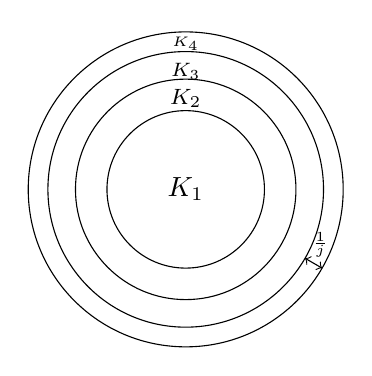
\begin{tikzpicture}
    
    \draw (0,0) circle (2);
    \draw (0,0) circle (1);
    \draw (0,0) circle (1.4);
    \draw (0,0) circle (1.75);
    
    \draw node at (0,0) {$K_1$};
    \draw node at (0,1.15) {\footnotesize $K_2$};
    \draw node at (0,1.5) {\scriptsize $K_3$};
    \draw node at (0,1.85) {\tiny $K_4$};
    \draw[<->] (-30:1.75) -- (-30:2);
    \draw node at (-22.5:1.851) {\tiny $\frac{1}{j}$};
    \draw [below right] node at (-45:2) {$\om$};
    
    
    \end{tikzpicture}
\end{center}
e.g. $K_j = \set{ z \in \C \mid dist(z,\partial \om) \geq \frac{1}{j} } \cap \overline{D_j(0)}$ (the disk of radius $j$ around the origin is to ensure boundedness). Now apply the first part of the proof to $K_1$ to get $\set{ f_{n,1} } $ a subsequence of $\set{f_n}$ s.t. $ f_{n,1}  \xrightarrow[]{\interior{C}(K_1)} f$, $f \in \interior{C} (K_1)$, $f$ holomorphic on $\interior{K}_{1}$. Now apply the first part of the proof to $K_2$ and the family $\set{ f_{n,1} }$. This yields a sub-subsequence $f_{n,2} \xrightarrow[]{\interior{C}(K_2)} \Tilde{f}$, $\Tilde{f} \in \interior{C}(K_2)$ holomorphic on $\interior{K}_{2}$. The uniform limit is unique, thus $f = \Tilde{f}$ on $K_1$ by uniform convergence.

Repeat this procedure to $\set{ f_{n,2} }$ on $K_3$ to get $\set{ f_{n,3} }$ etc. Finally take the sequence $\set{ f_{n,n} }_{n=0}^\infty$. By construction, $f_{n,n} \tou f$ on all compact subsets of $\om$.


This proves the first part of theorem (\ref{thm:montel}). The statement about the derivatives remains to be proved. For convenience, relabel so that $f_n \tou f$ on all compact subsets of $\om$. $\forall k \geq 0$, given any point $z_0 \in \om$, take $D = D_r(z) \ssubset \om$ for some $ r> 0$. Apply theorem (\ref{thm:cauchy-estimates}) to the function $f_n^{(k)} - f^{(k)}$:
\begin{align*}
    \forall z \in D_{\frac{r}{2}} (z_0) 
    \: z\abs{f_n^{(k)}(z) - f^{(k)} (z) } \leq \frac{k!}{r^k} \sup_{\partial D} \abs{f_n - f} \xrightarrow[]{f_n \xrightarrow[]{u} f} 0
\end{align*}
where $\sup_{\partial D} \abs{f_n - f} \to 0$ since $f_n \tou f$ on $\overline{D}$. Hence $f_n^{(k)} \to f^{(k)}$ locally uniformly $\implies$ $f_n^{(k)} \to f^{(k)}$ uniformly on all compact subsets of $\om$. This is what we wanted to prove, hence we are done.

\end{proof}

\subsection{Some Examples}

\begin{example}
For $C^\infty$ real functions this fails. Consider $f_n(x) = \sin(nx)$ on $[0,1] \subset \R$. Each $f_n$ is a uniformly bounded smooth function, but they are not equicontinuous, and in fact have no convergent subsequence on any compact subset of $[0,1]$.


\end{example}


\begin{example}

Consider $\oic$ open, $\om ' \subset \C$ open and bounded. Define 
\begin{align*}
    \F = \set{ f: \om \to \om ' \mid f \, holomorphic  }.
\end{align*} Then $\F$ is normal, as $\forall f \in \F, \, \sup_{\om} \abs{f} \leq diam(\om ')$, which is finite since $\om ' $ is bounded.

\end{example}


\begin{note}
The concept of normal families extends very easily to uncountable sets in the obvious way (still looking at countable sequences).
\end{note}

\begin{remark}
Part 3 of the proof of theorem (\ref{thm:montel}) shows that if $\F$ is a normal family of holomorphic function $\om \to \C$, then $\forall k\geq 0, \, \F^{(k)} = \set{f^{(k)} \mid f \in \F}$ is also normal. This will be used later in the course.
\end{remark}

We now move backwards in the textbook, back to our original location of chapter 3.


\section{Isolated Singularities, Poles}

Recall from last time: $\oic $ open connected, $\foc$ holomorphic, $f \nequiv 0$. Then given $z_0 \in \om, \exists D $ disk containing $z_0$. $\exists N \geq 0$ and holomorphic s.t. $g(w) \neq 0 \, \forall w \in D$ s.t. $f(z_0) = (z-z_0)^N \cdot g(z) $ on D.

Recall that we defined the unique $N$ in the previous section to be the order of vanishing, and that when $N=1$ we call $z_0$ a simple zero.


Say now that instead of a zero we have a singularity, $z_0 \in \om , \, f: \om \setminus \{ z_0 \} \to \C$ holomorphic on $\om \setminus \{ z_0 \}$.


\begin{center}
\begin{tikzpicture}
    \draw[shift={(-2.5,-2.5)},rotate=0][dotted][scale =2.5] plot [smooth cycle] coordinates {(0,0) (1,0.1) (2,0.3) (2,0.7) (1.5,1.5) (0.8,1.5) (0.3,1.2) (-0.2,0.6) };
    \draw (-2.25,-2.25) node {$\Omega$};
    
    \draw[thick] (-0.1,0.1) -- (0.1,-0.1);
    \draw[thick] (0.1,0.1) -- (-0.1,-0.1);
    \draw [below left] node at (0,0) {$z_0$};
    \draw[dotted] (0,0) circle (1);
    \draw [below right] node at (-30:1-0.05) {$D$};
    
\end{tikzpicture}    
\end{center}



\begin{definition}[Poles]
We say that $f$ has a \textbf{pole} at $z_0$ if $\exists \, D = D_r(z_0) \subset \om$ for some $r>0$ s.t. $f(z) \neq 0 \, \forall z \in D \setminus \{ z_0 \}$ and the function:

\begin{align*}
    \Tilde{f}(z) \vcentcolon = \begin{cases} \frac{1}{f(z)} & z \in D \setminus \{ z_0 \} \\ 0 & z = z_0  \end{cases}
\end{align*}

is holomorphic on $D$.

\end{definition}

To have a pole means to have a holomorphic function that is not defined at $z_0$  but is holomorphic outside, and must be non-zero on some punctured disk around $z_0$.



\begin{lemma}\label{lem:pole-lemma}
Suppose that $f$ has a pole at $z_0$. Then $\exists D \ni z_0$ disk, $\exists g: D \to \C $ holomorphic, $g(z) \neq 0 \, \forall z \in D$ and $\exists ! N \geq 1$ such that $\forall z\in D \setminus \{ z_0 \}$:
\begin{align*}
f(z) = \frac{g(z)}{(z-z_0)^N}.
\end{align*}

\end{lemma}

\begin{example}
$\frac{1}{z}$ at $z_0 = 0$ is the prototype of a pole.
\end{example}

\begin{example}
$\frac{1}{z^n}$, $n \geq 1$ at $z_0 = 0$ is also a pole.
\end{example}

\begin{proof}[\ref{lem:pole-lemma}]
Since $f$ has a pole, let $\tilde{f}$ be the function described above. $\tilde{f}: D \to \C$ holomorphic. By assumption $f$ is never $0$. Thus by construction, $\tilde{f}$ is non-zero except at the isolated zero $z_0$. By theorem (\ref{thm:isolated-zeroes}) from last time we can write:
\begin{align*}
    \tilde{f} (z) = (z-z_0)^N h(z) 
\end{align*}
on some possibly smaller disk at $z_0, \, N \geq 1$ and $h:D \to \C$ holomorphic and non-zero. Now we let:
\begin{align*}
    g(z) = \frac{1}{h(z)}
\end{align*}
and we are done.

\end{proof}

\begin{definition}[Order of Pole]
We call the unique $N$ in lemma (\ref{lem:pole-lemma}) the \textbf{order of the pole}. This is the analog to the order of the zero (the order of vanishing) defined in definition (\ref{def:order-vanish}). When $N=1$ we call it a simple pole.
\end{definition}


\begin{lemma}[Laurent Series for Poles]\label{lem:laurent-series}
Suppose that $f$ has a pole of order $N$ at $z_0 \in \om$ ($f$ is implicitly holomorphic on the punctured disk). Then $\exists D \ni z_0$ disk such that for $z\in \DP$:
\begin{align*}
    f(z) = \frac{a_{-N}}{(z-z_0)^N} + \frac{a_{-N+1}}{(z-z_0)^{N-1}} + \cdots + \frac{a_{-2}}{(z-z_0)^2} + \frac{a_{-1}}{z-z_0} + G(z)
\end{align*}

with $a_j \in \C, \, G(z) $ holomorphic on $D$. Thus we can effectively write for $z \in \DP$:

\begin{align*}
    f(z) = \sum_{n=-N}^\infty a_n (z-z_0)^n.
\end{align*}

This is the \textbf{Laurent series} of $f$ centered at $z_0$ (a pole).


\end{lemma}

\begin{proof}
Take lemma (\ref{lem:pole-lemma}). Then on $\DP$:
\begin{align*}
    f(z) = \frac{g(z)}{(z-z_0)^N} 
\end{align*}

Expand $g$ in power series on D:
\begin{align*}
g(z) = \sum_{n=0}^\infty A_n (z-z_0)^n
\end{align*}
and plug it in:
\begin{align*}
    f(z) &= \frac{1}{(z-z_0)^N} \cdot (A_0 + A_1(z-z_0) + A_2 (z-z_0)^2 + \cdots)\\
    \text{(letting $a_i = A_{i+N}$) } &= \sum_{n=-N}^\infty a_n (z-z_0)^n,
\end{align*}
and we are done.
\end{proof}

\begin{definition}[Principal Part and Residue]

When $f$ has a pole at $z_0$ we can write:
\begin{align*}
    f(z) = \sum_{n=-N}^{-1} a_n (z-z_0)^n + \sum_{n=0}^{\infty} a_n (z-z_0)^n
\end{align*}
The first sum is called the \textbf{principal part of $f$ at $z_0$}. $a_{-1} = \vcentcolon Res_{z_0} (f)$ is called the \textbf{residue of $f$ at $z_0$}. Note that $\abs{N} < \infty$.
\end{definition}

\begin{example}
The function
\begin{align*}
f(z) = \frac{1}{z+5}
\end{align*}
has a pole at $z_0 = -5$. The order of the pole is 1. This is the Laurent Series of $f$ at $z_0$, and thus $Rez_{-5}(f) = 1 $.
\end{example}



\begin{example}
The function
\begin{align*}
f(z) = \frac{1}{(z+5)^2}
\end{align*}
has a pole at $z_0 = -5$. The order of the pole is $2$. This is the Laurent Series of $f$ at $z_0$, and thus $Rez_{-5}(f) = 0 $.
\end{example}



\begin{example}
The function
\begin{align*}
f(z) = \frac{1}{z^2+1} = \frac{1}{(z-i)(z+i)}
\end{align*}
has two poles: $z = \pm i$. By plugging in $z= \pm i$ and ignoring the division by zero we get that:
\begin{align*}
    Res_i(f) &= \frac{1}{2i},\\
    Res_{-i}(f) &= \frac{-1}{2i}.
\end{align*}

\end{example}










%FILL IN THE RIGHT INFO.
%\lecture{**LECTURE-NUMBER**}{**DATE**}
\unchapter{Lecture 9}
\lecture{9}{October 1}
\setcounter{section}{0}
\setcounter{theorem}{0}

% **** YOUR NOTES GO HERE:


We spend more time on poles this lecture.

\section{Poles and the Residue Formula}

\begin{note}
Recall that a holomorphic function $f$ has a pole at $z_0$ if:

\begin{align*}
    \Tilde{f}(z) \vcentcolon = \begin{cases} \frac{1}{f(z)} & z \in D \setminus \{ z_0 \} \\ 0 & z = z_0  \end{cases}
\end{align*}

is holomorphic on $D$ (a disk around $z_0$). Naturally this implies that $lim_{z \to z_0} \frac{1}{f(z)} = 0$. This means that $lim_{z \to z_0} f(z) = \pm \infty$. This is to say that a pole is somehow a point where $f$ goes to $\pm \infty$.

\end{note}



We revisit an example from last lecture:





\begin{example}\label{ex:res-example}
The function
\begin{align*}
f(z) = \frac{1}{z^2+1} = \frac{1}{(z-i)(z+i)}
\end{align*}
has two poles: $z = \pm i$. Consider the pole $i$. Then:
\begin{align*}
    \frac{1}{z^2+1} = \frac{1}{(z-i)(z+i)} = \frac{\frac{1}{z+i}}{z-i} = \frac{g(z)}{z-z_0}
\end{align*}
for $z_0 = i$. $\frac{1}{z+i}$ is indeed a non-vanishing and holomorphic function around $i$. We then expand $g(z)$ in a power series at $z_0 = i$:
\begin{align*}
    g(z) = \sum _{n=0}^\infty a_n (z-i)^n &= a_0 + \cdots\\ &= \frac{1}{2i} + \cdots.
\end{align*}
Thus $a_{-1} = \frac{1}{2i}$ in the Laurent series expansion, so $Res_i(f) = \frac{1}{2i}$. Similarly, $Res_{-i}(f) = \frac{-1}{2i}$.
\end{example}

\begin{lemma}\label{lem:pole-res}
Say $f$ has a pole at $z_0 \in \om$ of order $N \geq 1$. Then:
\begin{align*}
    Res_{z_0}(f) = \lim_{z \to z_0} \left[ \frac{1}{(N-1)!} \left( \frac{\partial}{\partial z} \right)^{N-1} \left[ (z-z_0)^N \cdot f(z) \right] \right].
\end{align*}
\end{lemma}

\begin{note}
Multiplying by $(z-z_0)^N$ makes your function holomorphic. We then take the derivative and divide by $(N-1)!$ to readjust it after taking the derivative.
\end{note}

\begin{proof}[\ref{lem:pole-res}]
Expand $f$ by lemma (\ref{lem:laurent-series}). Then:
\begin{align*}
    f(z) &= \frac{a_{-N}}{(z-z_0)^N} + \cdots + \frac{a_{-1}}{z-z_0} + G(z)\\
    (z-z_0)^N f(z) &= a_{-N} + \cdots + (z-z_0)^{N-1} a_{-1} + (z-z_0)^N G(z).
\end{align*}

Then note that $(z-z_0)^N G(z)$ vanishes to order at least $N$ at the point $z_0$. Since taking the derivative reduces the order of vanishing by $1$, the $N-1$'th derivative of $(z-z_0)^N G(z)$ vanishes to order at least $1$ at the point $z_0$. Thus:
\begin{align*}
    \lim_{z \to z_0} \left[ \left( \frac{\partial}{\partial z} \right)^{N-1} \left[ (z-z_0)^N f(z)  \right] \right] &=  a_{-1} (N-1)! + \lim_{z \to z_0} \left[ \left( \frac{\partial}{\partial z} \right)^{N-1} \left[ (z-z_0)^N G(z) \right] \right]\\
    &= a_{-1}  (N-1)! + 0\\
    &= a_{-1}  (N-1)!.
\end{align*}
\end{proof}

\begin{example}
Consider:
\begin{align*}
    f(z) = \frac{e^z}{z^5} = \frac{g(z)}{z^5}.
\end{align*}

Then the denominator vanishes at $0$, and the numerator never vanishes. Thus $f$ has a pole of order $5$ at $z_0 = 0$. We approach this in two ways:
\begin{enumerate}
    \item We directly compute the residue. Expand $e^z = \sum \frac{z^n}{n!}$ as a power series around $z_0 = 0$. Then:
    \begin{align*}
        f(z) = \frac{1}{z^5} + \frac{1}{z^4} +\frac{1}{2z^3} + \frac{1}{6z^2} + \frac{1}{24z} + \cdots.
    \end{align*}
    We can directly observe that the residue is $\frac{1}{24}$.
    
    \item Use lemma (\ref{lem:pole-res}). Then $N=5$:
    
    \begin{align*}
        Res_{0}(f) &= \lim_{z \to 0} \frac{1}{4!} \left( \frac{\partial }{\partial z} \right)^4 e^z \\
        &= \lim_{z \to 0} \frac{1}{4!} e^z\\
        &= \frac{1}{4!}.
    \end{align*}
\end{enumerate}
\end{example}

\begin{lemma}\label{lem:res-lemma}
Suppose $f$ has a pole at $z_0 \in \om$ and expand $f(z) = \sum_{n=-N}^\infty a_n (z-z_0)^n$ in Laurent series around $z_0$ for some $D = D_r(z_0) \ssubset \om$. Then $\forall n$:
\begin{align*}
    a_n = \frac{1}{2 \pi i} \int_D \frac{f(z)}{(z-z_0)^{n+1}} \dif z.
\end{align*}
\end{lemma}

\begin{proof} On $\DP$:
\begin{align*}
    \frac{f(z)}{(z-z_0)^{n+1}} &= \sum_{j=-N}^\infty a_j (z-z_0)^{j-n-1}\\
    \int_D \frac{f(z)}{(z-z_0)^{n+1}} \dif z &= \sum_{j=-N}^\infty a_j \underbrace{\int_D (z-z_0)^{j-n-1} \dif z}_{2\pi i \text{ if } j-n-1=-1;\text{ 0 else}}\\
    &= a_n \cdot 2 \pi i.
\end{align*}

\end{proof}

We now present a theorem that is theoretically not very powerful, but is very useful for calculations:

\isubsection{THM: Residue Formula}

\begin{theorem}[Residue Formula]\label{thm:residue-formula}

Suppose $f$ holomorphic on $\om \setminus \set{ z_1,\cdots, z_N}, \, z_j \in \om $. Suppose that $f$ has poles at $z_1,\cdots, z_N$. Let $\om ' \ssubset \om$ open subset with piecewise smooth boundary with $z_1,\cdots, z_N \in \om '$. Then:
\begin{align*}
    \frac{1}{2\pi i} \int_{\partial \om '} f(z) \dif z = \sum_{i=1}^N Res_{z_i} (f).
\end{align*}

\end{theorem}

\begin{note}
Note that you don't have to have $\om ' \ssubset \om$, just that it's holomorphic on the closure of $\om$. Note that this also contains theorem (\ref{thm:cauchy-theorem}) as a trivial case (when $N$ = 0). In general there is no reason for the sum of the residues to be zero.
\end{note}





\begin{center}
\begin{tikzpicture}[
    tangent/.style={
        decoration={
            markings,% switch on markings
            mark=
                at position #1
                with
                {
                    \coordinate (tangent point-\pgfkeysvalueof{/pgf/decoration/mark info/sequence number}) at (0pt,0pt);
                    \coordinate (tangent unit vector-\pgfkeysvalueof{/pgf/decoration/mark info/sequence number}) at (1,0pt);
                    \coordinate (tangent orthogonal unit vector-\pgfkeysvalueof{/pgf/decoration/mark info/sequence number}) at (0pt,1);
                }
        },
        postaction=decorate
    },
    use tangent/.style={
        shift=(tangent point-#1),
        x=(tangent unit vector-#1),
        y=(tangent orthogonal unit vector-#1)
    },
    use tangent/.default=1
]
    \draw[dotted]
        plot [smooth cycle] coordinates {(-0.6*10,0) (-0.6*7,0.6*3.5) (0,0.6*5)  (0.6*4,0.6*2.5) (0.6*7,0)  (0.6*5,0.6*-7) (0.6*2,-0.6*6)  (-0.6*5,-0.6*5) };
    \draw[scale =0.5][tangent=0][tangent=0.1][tangent=0.15][tangent=0.3][tangent=0.4][tangent=0.5][tangent=0.6][tangent=0.7][tangent=0.8][tangent=0.9][tangent=1][tangent=1.1]
        plot [smooth cycle] coordinates {(-10,0) (-7,3.5) (0,5)  (4,2.5) (7,0)  (5,-7) (2,-6)  (-5,-5) } (0,0) circle (1) (170:5) circle (1) (-80:4) circle (1);
        
\draw [thick, use tangent=5][->] (0,0) -- (-0.01,0);
\draw [thick, use tangent=3][->] (0,0) -- (-0.01,0);
\draw [thick, use tangent=7][->] (0,0) -- (-0.01,0);

\draw [thick, use tangent=9][->] (0,0) -- (-0.01,0);
\draw [thick, use tangent=10][->] (0,0) -- (-0.01,0);
\draw [thick, use tangent=11][->] (0,0) -- (-0.01,0);


\draw[thick] (-0.1,0.1) -- (0.1,-0.1) (0.1,0.1) -- (-0.1,-0.1);
\draw (0,0) circle [radius=0.5];
\draw (0,0)[below] node {$z_1$};

\draw[shift=(170:2.5)][thick] (-0.1,0.1) -- (0.1,-0.1) (0.1,0.1) -- (-0.1,-0.1);
\draw (170:2.5) circle [radius=0.5];
\draw (170:2.5)[below] node {$z_2$};

\draw[shift=(-80:2)][thick] (-0.1,0.1) -- (0.1,-0.1) (0.1,0.1) -- (-0.1,-0.1);
\draw (-80:2) circle [radius=0.5];
\draw (-80:2)[below] node {$z_3$};

\draw node at (-3.75,-2) {$\Omega'$};
\draw node at (-4.3,-2.55) {$\Omega$};


\end{tikzpicture}

    
\end{center}





\begin{proof}
Apply theorem (\ref{thm:cauchy-theorem}) to some small disks around each pole. By assumption, $f$ is holomorphic on $\om ' \setminus \bigcup_{i=1}^N D_r(z_i)$ for some small $r>0$. Theorem (\ref{thm:cauchy-theorem}) applies on this new domain (parameterizing $\partial D_r(z_i)$ counterclockwise to achieve a negative):

\begin{align*}
    0 &= \int_{\partial \om '} f(z) \dif z - \sum_{j=1}^N \int_{\partial D_r(z_j)} f(z) \dif z\\
    \text{(apply lemma (\ref{lem:res-lemma})) } &= \int_{\partial \om '} f(z) \dif z - \sum_{j=1}^N 2\pi i \cdot Res_{z_j} (f).
\end{align*}

\end{proof}


\section{Applications of Residue Formula}

\begin{example}
$D = D_2(z)$. Compute $\int_{\partial D} \frac{z+1}{z^2 + 1 } \dif z$. This is hard to compute directly, but easy to do with residues. $f$ has two simple poles at $z_0 = \pm i$:
\begin{align*}
    \int_{\partial D} \frac{z+1}{z^2 + 1 } \dif z &= 2\pi i \left( Res_{i} \left( \frac{z+1}{z^2 + 1 } \right) + Res_{-i} \left( \frac{z+1}{z^2 + 1 } \right) \right)\\ \text{(from example (\ref{ex:res-example})) } &= 2\pi i \left( \frac{1+i}{2i} + \frac{-i+1}{-2i} \right) = 2 \pi i.
\end{align*}

\end{example}

\begin{example}
Evaluate $\int_{-\infty}^\infty \frac{\dif x }{ 1+ x^2}$. We use the contour of the  semicircle on the upper half plane of radius $R$.

\begin{center}
\begin{tikzpicture}[very thick,decoration={
    markings,
    mark=at position 0.6 with {\arrow{>}}}
    ]
    \clip (-4,-1.1) rectangle (4,4);
    %\draw (-4,-1) rectangle (4,4);
    \draw[postaction={decorate}][rotate = 200] [blue,line width=1.5pt] (0,0) circle [radius=3];
    
    \draw[color=white][fill=white] (-3.5,0) rectangle (3.5,-2);
    
    
    \draw [thin] [->] (-4,0)--(4,0);
    \draw [thin] [->] (0,-1)--(0,4);
    
    \draw[postaction={decorate}] [blue,line width=1.5pt] (-3-0.026,0) -- (3+0.026,0);
    
    %\draw[postaction={decorate}] [blue,line width=1.5pt] (-3,0) -- (3,0);
    %\draw[postaction={decorate}] [blue,line width=1.5pt] (3,2) -- (-3,2);
   % \draw[postaction={decorate}] [blue,line width=1.5pt] (3,0) -- (3,2);
    %\draw[postaction={decorate}] [blue,line width=1.5pt] (-3,2) -- (-3,0);
    
    
    \draw (-3,0)[below] node {$-R$};
    \draw (3,0)[below] node {$R$};
    
    \draw[thick] (-0.1,0.1+0.7) -- (0.1,-0.1+0.7);
    \draw[thick] (0.1,0.1+0.7) -- (-0.1,-0.1+0.7);
    
    \draw[thick] (-0.1,0.1-0.7) -- (0.1,-0.1-0.7);
    \draw[thick] (0.1,0.1-0.7) -- (-0.1,-0.1-0.7);
    
    
    \draw (-2,0)[below] node {$\gamma_1$};
    \draw (120:3)[above] node {$\gamma_2$};
    \draw (180-120:3)[above] node {$\gamma_R$};
    \draw (0,0.7) [above left] node {$i$};
    \draw (0,-0.7) [above left] node {$-i$};
    
    
    
    
\end{tikzpicture}
\end{center}

Now note that:
\begin{align*}
    \abs{f(z)} &= \frac{1}{\abs{a+z^2}} \leq \frac{2}{\abs{z}^2} = \frac{2}{R^2},\\
   \abs{ \int_{\gamma_2} \frac{\dif z }{ 1+ z^2} } &\leq L(\gamma_2) \cdot \frac{2}{R^2} = \pi R \frac{2}{R^2} \xrightarrow[]{R\to \infty} 0.
\end{align*}

Thus:
\begin{align*}
    \int_{\partial R} \frac{\dif z}{1+z^2} = \int_{\gamma_1} \frac{\dif z}{1+z^2} &+ \cancelto{0}{\int_{\gamma_2} \frac{\dif z}{1+z^2}} = 2\pi i \cdot \res{i}{\frac{1}{1+z^2}} = \pi.\\
    \implies \int_{\gamma_1} \frac{\dif z}{1+z^2} &= \int_{\R} \frac{\dif z}{1+z^2} = \pi.
\end{align*}

\end{example}



\begin{example}
Consider $\int_{-\infty}^\infty \frac{e^{ax}}{1+e^x} \dif x$. Note that $\left(\frac{e^{ax}}{1+e^x} \right) \xrightarrow[]{x \to \pm \infty} 0$. Thus $0 < a<1$ (otherwise the integral will diverge at $\pm \infty$).

We propose to use $f(z) = \frac{e^{ax}}{1+e^x}$. This has poles when $e^z = -1$, thus when $z = \pi i + 2 \pi i k, \, k \in \mathbb{Z}$.

We propose this contour:


\begin{center}
\begin{tikzpicture}[very thick,decoration={
    markings,
    mark=at position 0.6 with {\arrow{>}}}
    ]
    
    \draw [thin] [->] (-4,0)--(4,0);
    \draw [thin] [->] (0,-1)--(0,3);
    
    \draw[postaction={decorate}] [blue,line width=1.5pt] (-3,0) -- (3,0);
    \draw[postaction={decorate}] [blue,line width=1.5pt] (3,2) -- (-3,2);
    \draw[postaction={decorate}] [blue,line width=1.5pt] (3,0) -- (3,2);
    \draw[postaction={decorate}] [blue,line width=1.5pt] (-3,2) -- (-3,0);
    
    
    \draw (-3,0)[below] node {$-R$};
    \draw (3,0)[below] node {$R$};
    \draw (3,2)[above] node {$R+2 \pi i$};
    \draw (-3,2)[above] node {$-R+2 \pi i$};
    
    \draw (1,0)[below] node {$\gamma_1$};
    \draw (3,1)[right] node {$\gamma_2$};
    \draw (-1,2)[above] node {$\gamma_3$};
    \draw (-3,1)[left] node {$\gamma_4$};
    
    
    \draw[thick] (-0.1,0.1+1) -- (0.1,-0.1+1);
    \draw[thick] (0.1,0.1+1) -- (-0.1,-0.1+1);
    \draw (0,1) [above right] node {$\pi i$};
    
\end{tikzpicture}
\end{center}

By the residue formula:
\begin{align*}
    \int_{\gamma_1} + \int_{\gamma_2} + \int_{\gamma_3} + \int_{\gamma_4} = 2 \pi i \cdot \res{\pi i}{f}.
\end{align*}

Since these are simple poles:
\begin{align*}
    \res{\pi i}{f} &= \lim_{z \to \pi i} (z - \pi i) f(z)\\
    &= \lim_{z \to \pi i} \frac{e^{az} (z-\pi i)}{1+e^z}.
\end{align*}

We expand the denominator using $h(z) = e^z$ at $z_0 = \pi i$ :
\begin{align*}
    h(z) &= h(z_0) + h'(z_0)(z-z_0) + o( \, \abs{z-z_0})\\
    &= e^{\pi i} + e^{\pi i} (z- \pi i) +  o( \, \abs{z-\pi i})\\
    &= -1 -(z-\pi i) + o( \, \abs{z-\pi i}).\\
    e^z + 1 &= -(z-\pi i) + o( \, \abs{z-\pi i}).
\end{align*}

Thus:
\begin{align*}
    \res{\pi i}{f} &= \lim_{z \to \pi i} \frac{e^{az} (z-\pi i)}{1+e^z}\\
    &= \lim_{z \to \pi i} \left( -e^{az} + o(1) \right) = - e^{a\pi i}.
\end{align*}

Evaluating the $\gamma_1$ term:
\begin{align*}
    \int_{\gamma_1} f(z) \dif z &= \int_{-R}^R \frac{e^{ax}}{1+e^x} \dif x \xrightarrow[]{R \to \infty } \int_{-\infty}^\infty \frac{e^{ax}}{1+e^x} \dif x.
\end{align*}

Evaluating the $\gamma_3$ term, remaining conscious of the fact that $\gamma_3$ is $\gamma_1$ evaluated backwards but shifted up $2 \pi i$:
\begin{align*}
    \int_{\gamma_3} f(z) \dif z &= \int_{\gamma_3} \frac{e^{az}}{1+e^z} \dif z\\
    &= \int_{\gamma_1} \frac{e^{a(z+2\pi i)}}{1+e^{(z+2\pi i)}} \dif z\\
    &= - e^{2\pi i a} \int_{\gamma_1}  f(z) \dif z.
\end{align*}
 Where the minus sign is because we parameterize $\gamma_3$ in the opposite direction compared to $\gamma_1$, and the factor of $e^{2\pi i a}$ comes from the fact that the parameterization of $\gamma_3$ involves adding $2\pi i$ to the parameterization of $\gamma_1$.

Evaluating the $\gamma_2$ term with parameterization $z(t) = R + it, \, t \in [0,2\pi ]$:
\begin{align*}
    \abs{\int_{\gamma_2} f(z) \dif z }&=\abs{ \int_0^{2\pi} \frac{e^{a(R+it)}}{1+e^{R+it}} i \dif t }\\
    &\leq  \int_0^{2\pi} \abs{ \frac{e^{a(R+it)}}{1+e^{R+it}} i} \dif t \\
    &= \int_0^{2\pi} \frac{e^{aR}}{\abs{ 1+e^{R+it} }} \dif t\\
    &\leq \int_0^{2\pi}  \frac{e^{aR}}{e^R -1 }       \dif t\\
    \text{(for some constant C) }&\leq \int_0^{2\pi}  C e^{(a-1)R}       \dif t \xrightarrow[]{R \to \infty} 0.
\end{align*}

Similarly for $\gamma_4$ with parameterization $z(t) = -R - it, \, t \in [0,2\pi ]$:
\begin{align*}
    \abs{\int_{\gamma_4} f(z) \dif z } &=\abs{ \int_0^{2\pi} \frac{e^{-a(R+it)}}{1+e^{-(R+it)}} i \dif t }\\
    &\leq \int_0^{2\pi} \abs{\frac{e^{-a(R+it)}}{1+e^{-(R+it)}}}  \dif t\\
    \text{(for some constant C) } &\leq \int_0^{2\pi} Ce^{-aR}  \dif t \xrightarrow[]{R \to \infty} 0.
\end{align*}

Finally this implies that, since $\sin(z)  = \frac{e^{iz} - e^{-iz}}{2 i}$:
\begin{align*}
    - 2 \pi i e^{a\pi i} &= (1-e^{2\pi i a}) \int_\R \frac{e^{ax}}{1+e^x} \dif x.\\
    \implies \int_\R \frac{e^{ax}}{1+e^x} \dif x &= \frac{2\pi i}{e^{\pi ia} - e^{-\pi i a}} = \frac{\pi}{\sin(\pi a)}.
\end{align*}

And thus we are done.

\end{example}
%FILL IN THE RIGHT INFO.
%\lecture{**LECTURE-NUMBER**}{**DATE**}
\unchapter{Lecture 10}
\lecture{10}{October 6}
\setcounter{section}{0}
\setcounter{theorem}{0}

% **** YOUR NOTES GO HERE:

We go into more depth on isolated singularities of functions.


Let $\oic$ open, $z_0 \in \om$, $f: \omP \to \C$ holomorphic. Then $z_0$ is a possible isolated singularity of $f$.


\begin{definition}[Singularity]

Let $\oic$ open, $z_0 \in \om$, $f: \omP \to \C$ holomorphic. $z_0$ is said to be a \textbf{singularity} of $f$ if $f$ cannot be extended to a holomorphic function over all of $\om$ (especially at $z_0$).

\end{definition}


\begin{theorem}
Let $0 \leq r < R $. Consider $A = \set{ z\in \C \, \mid \, r< \abs{z-z_0} <R }$ (when $r=0$ this gives you a punctured disk). Let $f: A \to \C$ holomorphic. Then for every $r<r'<R'<R$, we can write $f$ as a Laurent series:
\begin{align*}
    f(z) &= \sum_{-\infty}^\infty a_n (z-z_0)^n & r' \leq \abs{z-z_0} \leq R',
\end{align*}
and this series is absolutely convergent on this smaller annulus $\set{ z\in \C \, \mid \, r'< \abs{z-z_0} <R' }$ and $\forall u \in (r,R)$:
\begin{align*}
    a_n = \frac{1}{2 \pi i} \int_{\abs{z-z_0}=u} \frac{f(w)}{(w-z_0)^{n+1}} \dif w.
\end{align*}
\end{theorem}


\begin{center}
\begin{tikzpicture}[scale = 1.5]
    \draw[shift={(-2.5,-2)},rotate=0][dotted][scale =2.5] plot [smooth cycle] coordinates {(0,0) (1,0.1) (2,0.3) (2,0.7) (1.5,1.5) (0.8,1.5) (0.3,1.2) (-0.2,0.6) };
    
    
    \draw [pattern=north west lines][dotted][thick]  (0,0) circle (1.4);
    \draw [fill=white][dotted][thick]  (0,0) circle (0.6);
    
    \draw (0,0) -- (-40:1.4);
    \draw (0,0) -- (40:0.6);
    
    \draw[above left] (40:0.3) node {$r$};
    \draw[->] (0: 1.8) to [out=190,in=40] (-40:1);
    \draw[above] (0: 1.8) node {$R$};
    
    \draw[fill] (0,0) circle (0.02);
    \draw[left] (0,0) node {$z_0$};
    
\end{tikzpicture}    
\end{center}


\begin{note}
When we say that $\sum_{-\infty}^\infty a_n (z-z_0)^n$ is absolutely convergent we mean that both $\sum_{0}^\infty a_n (z-z_0)^n$ and $\sum_{-\infty}^0 a_n (z-z_0)^n$ are absolutely convergent.
\end{note}

\begin{example}
Consider $f(z) = e^{\frac{1}{z}}$ on $\C^* = \C \setminus \{ 0 \}$. The Laurent series on any annulus $\set{r < \abs{z} < R}$ is given by:
\begin{align*}
    f(z) = \sum_{n=0}^\infty \frac{z^{-n}}{n!}.
\end{align*}

\end{example}

\begin{proof}
On smaller annulus, $f$ is holomorphic by assumption, so we apply equation (\ref{eq:cauchy-int-fla}). Noting that $r' \leq \abs{z-z_0} \leq R'$:








\begin{center}
\begin{tikzpicture}[decoration={
    markings,
    mark=at position 0.5 with {\arrow{>}}}
    ]
    
    \draw [dotted] (0,0) circle [radius=2.8];
    \draw[postaction={decorate}][pattern=north west lines][rotate = -120] (0,0) circle [radius=2.4];
    
    \draw[postaction={decorate}][fill = white][xscale=-1][rotate = -60] (0,0) circle [radius=1.2];
    \draw [dotted] (0,0) circle [radius=1];
    
    
    \draw[above left] (40:0.6) node {$r'$};
    
    \draw[above] (0: 3.6) node {$R'$};
    
    \draw[fill] (0,0) circle (0.02);
    \draw[left] (0,0) node {$z_0$};
    \draw[->] (0: 3.6) to [out=190,in=40] (-40:2);
    \draw (0,0) -- (-40:2.4);
    \draw (0,0) -- (40:1.2);
    
\end{tikzpicture}
\end{center}















\begin{align*}
    f(z) &= \frac{1}{2 \pi i} \int_{\abs{w- z_0} = R} \frac{f(w)}{w-z} \dif w - \frac{1}{2 \pi i} \int_{\abs{w- z_0} = r} \frac{f(w)}{w-z} \dif w.
\end{align*}
Using the fact that $w-z = w-z_0 -(z-z_0) = (z-z_0) \left( \frac{w-z_0}{z-z_0} -1 \right)$:
\begin{align*}
    f(z) &= \sum_{n=0}^\infty a_n (z-z_0)^n - \frac{1}{2 \pi i} \int_{\abs{w- z_0} = r} \frac{f(w)}{w-z} \dif w,\\
    \text{with } a_n &= \frac{1}{2 \pi i} \int_{\abs{w- z_0} = R} \frac{f(w)}{(w-z_0)^{n+1}}. \dif w
\end{align*}
Note that we cannot use the same trick for the second term since $f$ is not holomorphic inside the disk (so the power series does not converge in it). We can still do something similar. Noting that:


\begin{center}
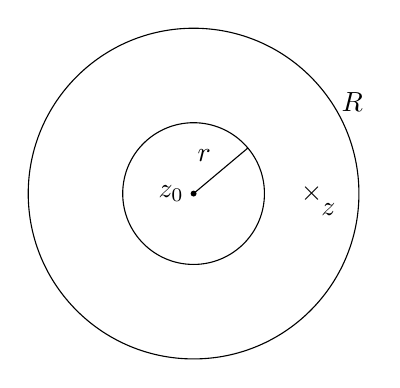
\begin{tikzpicture}[scale = 1.5]

    
    
    \draw  (0,0) circle (1.4);
    \draw [fill=white]  (0,0) circle (0.6);
    
    \draw (0,0) -- (40:0.6);
    
    \draw[above left] (40:0.3) node {$r$};
    \draw (30: 1.55) node {$R$};
    
    \draw[fill] (0,0) circle (0.02);
    \draw[left] (0,0) node {$z_0$};
    
    \draw[below right] (0: 1) node {$z$};
    \draw (0: 1) node {$\times$};
    
\end{tikzpicture}    
\end{center}


\begin{align*}
    w-z &= - (z-z_0) \left(   1-  \frac{w-z_0}{z-z_0} \right),\\
\text{and that } \abs{\frac{w-z_0}{z-z_0}} &\leq \frac{r}{r'} < 1,
\end{align*}
we get that:
\begin{align*}
    -\frac{1}{w-z} &= \frac{1}{z-z_0} \cdot \frac{1}{1-\frac{w-z_0}{z-z_0}}\\ &= \frac{1}{z-z_0} \cdot \sum_{n=0}^\infty \left( \frac{w-z_0}{z-z_0} \right)^n\\
    &= \sum_{n=0}^\infty \frac{(w-z_0)^n}{(z-z_0)^{n+1}}\\
    \text{(relabel) } &= \sum_{n=0}^{-\infty} \frac{(z-z_0)^{n-1}}{(w-z_0)^n}\\
    \text{(relabel) } &= \sum_{n=-1}^{-\infty} \frac{(z-z_0)^{n}}{(w-z_0)^{n+1}}.
\end{align*}

This new representation of $\frac{-1}{w-z}$ has strictly negative powers of $(z-z_0)$, exactly what we want:
\begin{align*}
    f(z) &= \sum_{n=0}^\infty a_n (z-z_0)^n - \frac{1}{2 \pi i} \int_{\abs{w- z_0} = r} \frac{f(w)}{w-z} \dif w\\
    &= \sum_{n=0}^\infty a_n (z-z_0)^n + \sum_{n=-1}^{-\infty} a_n (z-z_0)^n,
\end{align*}
where the $a_n$ in the second part of the sum comes from the same formula that gave us $a_n$ in the first part of the sum: $a_n = \frac{1}{2 \pi i} \int_{\abs{w- z_0} = r} \frac{f(w)}{(w-z_0)^{n+1}} \dif w$. Note that you can use any radius you want that is in the annulus, especially $r$ and $R$. The integral evaluates to the same thing by theorem (\ref{thm:cauchy-theorem}).
\end{proof}


\begin{remark}
In the case of poles we get the same Laurent series that we had before (ie $\sum_{-N}^\infty a_n (z-z_0)^n$). This theorem says that for a general holomorphic function the index of the sum can extend backwards to $-\infty$.
\end{remark}


Laurent series allow us to study isolated singularities. 

\section{Classification of Singularities}
\isubsection{THM: Riemann Extension Theorem}
\begin{theorem}[Riemann Extension Theorem]\label{thm:r-extension-thm}
Let $\oic$ open , $z_0\in \om$, $f: \omP \to \C$ holomorphic. Suppose that $\sup_{\omP}\abs{f} < \infty$. Then $\exists ! \Tilde{f}: \om \to \C$ holomorphic s.t. $\Tilde{f}\mid_{\omP} = f$.
\end{theorem}

\begin{definition}[Removable Singularities and Holomorphic Extensions]
We call this $\Tilde{f}$ a \textbf{holomorphic extension} of $f$ across $z_0$, and we will say that $z_0$ is a \textbf{removable singularity} of $f$.

\end{definition}



\begin{remark}
If $\Tilde{f}: \om \to \C$ holomorphic and we call $f=\Tilde{f}\mid_{\omP}$ then obviously $\sup_{D_r(z_0)\setminus \{z_0\} } \abs{f} < \infty$ for $r$ small, thus boundedness of $\, \abs{f}$ is necessary and sufficient for $z_0$ being a removable singularity.
\end{remark}

\begin{proof}[\ref{thm:r-extension-thm}]
Let $R>0$ small enough such that $D_R(z_0) \ssubset \om$, and so $\abs{f(z) } \leq C$ for some $C>0$, $\forall z$ such that $0 < \abs{z-z_0} < R$. Expand $f$ in Laurent series on this annulus:
\begin{align*}
    f(z) &= \sum_{-\infty}^\infty a_n (z-z_0)n,\\
    \text{with } a_n &= \int_{\abs{w-z_0} = R} \frac{f(w)}{(w-z_0)^{n+1}} \dif w.
\end{align*}

So for $n = -m$, $m > 0$ (ie $n<0$):
\begin{align*}
    \abs{a_{-m}} &\leq \frac{1}{2 \pi } \cdot \abs{\int_{\abs{w-z_0} =R} \frac{f(w)}{(w-z_0)^{-m+1}}  \dif w}\\
    &= \frac{1}{2 \pi } \cdot \abs{\int_{\abs{w-z_0} =R} f(w)(w-z_0)^{m-1}  \dif w}\\
    \text{let ($w(t) = z_0 +Re^{it}$) } &= \abs{\int_{\abs{w-z_0} =R} f(z_0 +Re^{it})R^{m-1} +Re^{i(m-1)t} Ri e^{it}  \dif t}\\
    &\leq R^m \cdot C \xrightarrow[]{R\to 0} 0.
\end{align*}

Where the final line comes from the fact that $\abs{f}$ is bounded, and the fact that $\abs{e^{ix}} = 1$. Thus letting $R \to 0$ we get that $\abs{a_{-m}} = 0 \, \forall m>0$. Thus the Laurent series has no negative powers.

Let $\Tilde{f}(z) = \sum_{n=0}^\infty a_m (z-z_0)^n$ on $D_R(z_0)$. This agrees with $f$ on $D_R(z_0) \setminus \{ z_0 \}$, so we get a holomorphic extension of $f$ across $z_0$. The uniqueness of $\Tilde{f}$ was already discussed (compare to analytic continuation).
\end{proof}

\begin{corollary}
$f: \omP \to \C$ holomorphic. $f$ has a pole at $z_0$ iff $\abs{f(z)} \xrightarrow[]{z \to z_0} \infty$.
\end{corollary}

\begin{proof}
\begin{enumerate}
    \item[$\Rightarrow$] By definition of pole, $\frac{1}{f(z)}$ (well-defined near $z_0$) has a zero at $z_0$. Thus $\abs{\frac{1}{f(z)}} \xrightarrow[]{z\to z_0}0$ which implies that $\abs{f(z)} \xrightarrow[]{z\to z_0} \infty$.
    
    \item[$\Leftarrow$] Since $f$ goes to infinity near $z_0$, $f(z) \neq 0$ $ \forall z \in D_r(z_0) \setminus \{ z_0 \}$ for some $r>0$ small. Thus $\frac{1}{f(z)}$ is holomorphic on $D_r(z_0) \setminus \{ z_0 \}$ and $\sup_{D_r(z_0) \setminus \{ z_0 \}} \frac{1}{\abs{f(z)}} \leq C$ since $\abs{f} \to \infty$.
    
    Since $\frac{1}{f(z)}$ is holomorphic and bounded, theorem (\ref{thm:r-extension-thm}) applies to it. Thus $z=z_0$ is a removable singularity of $\frac{1}{f(z)}$, and since $\abs{f} \to \infty$ then $\abs{\frac{1}{f}} \xrightarrow[]{z\to z_0} 0$. Thus the holomorphic extension of $\frac{1}{f(z)}$ at $z_0$ has value 0. Thus $z_0$ is a pole of $f$.
\end{enumerate}
\end{proof}

We can now examine the 3 different kinds of poles.

\subsection{Types of Poles}

\begin{definition}
$z_0 \in \om$, $f: \omP \to \C$ holomorphic ($z_0$ is a singularity of $f$).

There are three mutually exclusive cases:
\begin{enumerate}
    \item $z_0$ is a \textbf{removable singularity} of $f$ $\iff$ $\abs{f} < C$ near $z_0$ (iff by theorem (\ref{thm:r-extension-thm})),
    
    \item $z_0$ is a \textbf{pole} of $f$ $\iff$ $\abs{f} \xrightarrow[]{z\to z_0} \infty$,
    
    \item $z_0$ is an \textbf{essential singularity} of $f$ $\iff$ $z_0$ is neither removable nor a pole.
\end{enumerate}
\end{definition}

\begin{example}
$f(z) = e^{\frac{1}{z}}$ has an essential singularity at $z_0 = 0$. Consider $\abs{e^{\frac{1}{z}}}$ as $z\to 0$:
\begin{enumerate}
    \item[$0<z \in \R$:] $e^{\frac{1}{z}} \xrightarrow[]{x \to 0} +\infty$\\
    \item[$0>z \in \R$:] $e^{\frac{1}{z}} \xrightarrow[]{x \to 0} 0$\\
    \item[$z = iy,\, y \in \R$:] $\abs{e^{\frac{-i}{y}}}$ = 1 (however the argument varies wildly)
\end{enumerate}

Thus this is neither a pole nor a removable singularity.
\end{example}

You can detect the type of singularity by examining the Laurent series:

\begin{note}
Let $f(z) = \sum_{n=-\infty}^\infty a_n (z-z_0)^n$. Three distinct cases:

\begin{enumerate}
    \item $f(z) = \sum_{n=0}^\infty a_n (z-z_0)^n$. This implies $z_0$ is a removable singularity.
    
    \item $f(z) = \sum_{n=-N}^\infty a_n (z-z_0)^n$. This implies $z_0$ is a pole.
    
    \item $f(z) = \sum_{n=-\infty}^\infty a_n (z-z_0)^n$. This implies $z_0$ is an essential singularity.
\end{enumerate}


\end{note}

\isubsection{THM: Casorati-Weierstra{\ss}}
\begin{theorem}[Casorati-Weierstra{\ss}]\label{thm:caso-weier}
Suppose $f: \omP \to \C$ holomorphic and $z_0$ an essential singularity. Then $\forall r> 0$ small such that $D_r(z_0) \subset \om$, we have that $f(D_r(z_0) \setminus \{ z_0 \})$ is dense in $\C$.
\end{theorem}

%ADD A DRAWING MAYBE? I CANNOT DRAW DENSE SETS


\begin{proof}
Suppose that $A = f(D_r(z_0) \setminus \{ z_0 \})$ is not dense. Then $\overline{A} \neq \C$. Thus $\exists w \in \C$, $w \notin \overline{A} $. Then  $w$ has positive distance from $\overline{A}$, ie $\exists \delta >0$ s.t. $\abs{f(z) - w} > \delta$, $\forall z \in A$. Let $g(z) = \frac{1}{f(z) - w}$, $z \in A$ (this is okay since we know that $\abs{f(z) - w} > 0$). This is holomorphic on $A$ with $g \neq 0$ on the punctured disk.

Then $\abs{g(z)} < \frac{1}{\delta} \, \forall z \in A$, so $z_0$ is a removable singularity for $g$. Two cases follow:


\begin{enumerate}
    \item[$g(z_0) \neq 0$:] $g(z) = \frac{1}{f(z) - w}$, $g(z) \neq 0$ near $z_0$, thus we take $\frac{1}{g(z)} + w = f(z)$. Since this is a sum of two holomorphic functions, $f$ is also holomorphic at $z_0$. Thus $z_0$ is a removable singularity of $f$, which is absurd.
    \item[$g(z_0) = 0$:] Then since $g\neq 0$,  $z_0$ is an isolated zero of $g$ with an order of vanishing of $N \geq 1$. So $f(z) = w + \frac{1}{g(z)}$. This is holomorphic on $A$ as the sum of two functions that are holomorphic on $A$. Since $\frac{1}{g(z)}$ has a pole at $z_0$, so does $f(z)$, which is absurd.
\end{enumerate}





\end{proof}



\begin{remark}
We have a trichotomy of singularities. Removable singularities are in a sense not real singularities. Poles are our friends; they have residues and we can use the residue formula on them. Essential singularities are wild and bad, and behave very badly.
\end{remark}

Poles are special enough that we give a name to functions that are composed of only poles for singularities.


\begin{definition}[Meromorphic Functions]
A function $f$ on $\om$ open is called \textbf{meromorphic} if there is a countable collection $\{ z_i \}_{i=0}^\infty \subset \om$ of points with no accumulation point inside $\om$ (accumulation points on the boundary is possible), and $f: \om \setminus \bigcup_{j=0}^\infty \{ z_j \} \to \C $ holomorphic function such that $z_j$'s are all poles of $f$.
\end{definition}




%FILL IN THE RIGHT INFO.
%\lecture{**LECTURE-NUMBER**}{**DATE**}
\unchapter{Lecture 11}
\lecture{11}{October 8}
\setcounter{section}{0}
\setcounter{theorem}{0}

% **** YOUR NOTES GO HERE:



\section{Meromorphic Functions}

We start by giving an examples of meromorphic functions (defined at the end of last class).

\begin{example}[Meromorphic Functions]
\hphantom{M} %for formatting
\begin{enumerate}
    \item Anything that we have already seen with a pole.
    \begin{center}
        e.g. $\frac{1}{z}$, $\frac{1}{z^2}$, $\frac{1}{z^2+1}$, $\frac{1}{(z-5)^3}$, $\cdots$
    \end{center}
    
    \item Rational functions (a ratio of two finite polynomials)
    \begin{center}
        e.g. $\frac{z}{z^2+1}$, $\frac{1+z+z^2}{(z-1)^2}$, $\frac{z-4}{z+5}$, $\cdots$
    \end{center}
    
    \item Ratio of two holomorphic functions (with denominator $\not\equiv 0$)
    \begin{center}
        e.g. $\frac{e^z}{z^2+1}$, $\frac{z^5+2}{\cos(z)}$, $\cdots$
    \end{center}
\end{enumerate}

\end{example}

\begin{note}
Case 2 follows from case 3 as a special case. We will now prove case 3.
\end{note}

\begin{proposition}
The ratio of two holomorphic functions $\frac{f(z)}{g(z)}$, with $g(z) \not\equiv 0$, is a meromorphic function.
\end{proposition}

\begin{proof}
$f,g$ holomorphic. Thus $\frac{f(z)}{g(z)}$ is holomorphic at all $z$ s.t. $g(z) = 0$. The zeroes of $g$ are isolated. Let $z_0$ be a point where $g$ vanishes. Let $N \geq 1$ be the order of vanishing of $g$ at $z_0$. If $f\equiv 0$ we are done. Thus there are three cases to consider:

\begin{enumerate}
    \item \fbox{$f(z_0) \neq 0$}:
    
    Then we can consider the reciprocal $\frac{g(z)}{f(z)}$. This is non-zero in $\DrP{r}{z_0}$ for some $r>0$. This new function has a zero of order $N$ at $z_0$. By definition, $\frac{f(z)}{g(z)}$ has a pole at $z_0$ of order $N$.
    
    \item \fbox{$f(z_0) = 0$ with order $M<N$}:
    
    Then we write $f(z) = h_1(z) \cdot (z-z_0)^M$ and $g(z) = h_2(z) \cdot (z-z_0)^N$ near $z_0$ with $h_1,h_2$ holomorphic on $D_r(z_0)$. Then $\frac{f(z)}{g(z)} = \frac{h_1(z) \cdot (z-z_0)^M}{h_2(z) \cdot (z-z_0)^N} = \frac{h_1(z)}{h_2(z)} \cdot \frac{1}{(z-z_0)^{N-M}}$, which is a pole of order $N-M$.
    
    \item \fbox{$f(z_0) = 0$ with order $M\geq N$}:
    
    Then, following exactly from case 2, we write $\frac{f(z)}{g(z)} = \frac{h_1(z)}{h_2(z)} \cdot (z-z_0)^{M-N}$, which is holomorphic at $z_0$ with a removable singularity.
    
\end{enumerate}


Thus $\frac{f(z)}{g(z)}$ is meromorphic with every pole being a zero of $g(z)$.
\end{proof}

\begin{note}
    This is the most general formulation of a meromorphic function.
\end{note}

\section{Point at Infinity}

Consider $\C$. $\C$ is not compact, but we can add a single point (our so called ``$\infty$") and define a topology on $\C \cup \set{ \infty }$ such that it is compact.


\begin{definition}[Neighborhood of $\infty$]
A \textbf{neighborhood of $\infty$} is a set $U \subset \C$ open such that $\set{\abs{z} > R} \subset U$ for some $R > 0$
\end{definition}


%[view top right]
\begin{center}

\begin{tikzpicture}


    \draw (0, 3.5, 0) node {$\times$};
    \draw [below right] (0, 3.5, 0) node {$\infty$};
    
    \draw [black][pattern=north west lines] [dotted]
      (-5, 0, -3) -- (-5, 0, 3)
      -- (5, 0, 3) -- (5, 0, -3)
      -- cycle;

    \draw [fill=white] (0, 0, 0) [y={(0,0,1)}] circle (1.5);
    \draw (0,0,0) -- (0,0,1.5);
    \draw [right] (0,0,1.5/2) node {$R$};
    \draw [below right] (5, 0, 0) node {$\C$};
    \draw[->] (3, 1.5, -2) to [out=240,in=120] (3, 0, -2);
    \draw [above] (3, 1.5, -2) node {$\abs{z}>R$};
    
    \draw [fill] (0,0) circle [radius=0.04];
    \draw [above left] (0,0) node {$0$};
    %\draw [color=red][pattern=north west lines][dotted][thick]  (0,0) circle (1.4);
        
     %   \draw [color=red][fill=white][dotted][thick] (50:0.7) circle (0.4);
  \end{tikzpicture}

    
\end{center}




\begin{center}
    $\Downarrow$
\end{center}





\begin{center}
    
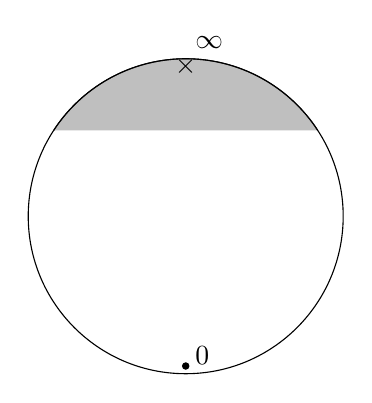
\begin{tikzpicture} % MERC

\def\angEl{18} % elevation angle. Change this for a different angle. DONT CHANGE ANYTHING ELSE UNLESS YOU HAVE OVER 500IQ

\pgfmathsetmacro\H{2*cos(\angEl)}

\fill[white] (0,0) circle (2); % just a white circle

\draw (0,0) circle (2);

\draw[fill=gray,fill opacity=0.5] (0,0,0) ++(33:2cm) arc (33:180-33:2);
\DrawLatitudeCircleF[2]{33}
\DrawLatitudeCircle[2]{0} % equator
\draw (0,\H) node {$\times$};
\draw [above right] (0, \H+0.1) node {$\infty$};

\draw [fill] (0,-\H) circle [radius=0.04];
\draw [above right] (0, -\H-0.1) node {$0$};


\end{tikzpicture}

\end{center}



























If $f:U \to \C$ holomorphic where U is a neighborhood of $\infty$, we can consider $F(z) = \frac{1}{f(z)}$, a holomorphic function on $\set{\abs{z} < \frac{1}{R}} \setminus \{ 0 \}$, a punctured neighborhood around $0$. This set is obtained by taking the reciprocal of $\abs{z}$ in the above definition on $U$. Thus switching $z$ with $\frac{1}{z}$ in some way swaps $\infty$ with $0$.

\begin{definition}
Consider a function $f(z)$ and the function $F(z) = f(\frac{1}{z})$. We say that:
\begin{itemize}
    \item $f$ is \textbf{holomorphic at $\infty$} if $F$ has a removable singularity at $0$.
    \item $f$ has a \textbf{pole of order $N$ at $\infty$} if $F$ has a pole at $0$ of order $N$.
    \item $f$ has an \textbf{essential singularity at $\infty$} if $F$ has an essential singularity at $0$.
    \item $f$ meromorphic on $U$ is \textbf{meromorphic at $\infty$} if $f$ does not have an essential singularity at $\infty$.
\end{itemize}
\end{definition}


\begin{example}
It is easy to get lost in the definition of $F$; take care not to.
\begin{itemize}
    \item $e^{\frac{1}{z}}$, which has an essential singularity at $0$, is holomorphic at $\infty$. This is because $F(z) = e^z$ is holomorphic at $0$.
    
    \item $z^2$, and entire holomorphic function, has a pole at $\infty$ of order 2. This is because $F(z) = \frac{1}{z^2}$ has a pole of order $2$ at $0$.
    
    \item $e^z$ has an essential singularity at $\infty$.
\end{itemize}
\end{example}

\isubsection{THM:Characterization of Rational Functions}

\begin{theorem}[Characterization of Rational Functions]\label{thm:char-rat}

Suppose $f $ meromorphic on $\C$ and $f $ meromorphic at $\infty$. 
Then $f$ is a rational function ($f(z) = \frac{P(z)}{Q(z)}, \, P,Q \in \C [z], \, Q \nequiv 0$).
\end{theorem}

\begin{note}
This theorem means that we can classify meromorphic functions as rational iff they are meromorphic at $\infty$. This is significant since the set of polynomials is much smaller than the set of all meromorphic functions. This also implies that almost all meromorphic functions will have an essential singularity at $\infty$ (since few are rational, and all others must have an essential singularity at $\infty$).
\end{note}

\begin{proof}[\ref{thm:char-rat}]
Let $f$ meromorphic on $\C$. Then the poles of $f$ do not accumulate in $\C$. The poles of $f$ cannot accumulate at $\infty$ since $f$ is meromorphic at $\infty$ (since $f(\frac{1}{z})$ has a pole or removable singularity at $0$, it will be holomorphic and non-zero in $\DrP{r}{0}$ for some $r>0$, so $f$ has no poles in some punctured neighborhood of $\infty$). 

It follows that since they cannot accumulate anywhere, $f$ has finite poles $\set{z_1, \cdots ,z_n}$ (and possibly $\infty$). Let $z_k$ be a pole in $\C$. Write for $z$ near $z_k$:
\begin{align*}
    f(z) = \underbrace{f_k(z)}_{principal} + \underbrace{g_k(z)}_{hol'c}
\end{align*}
with $g_k(z)$ a polynomial in $\frac{1}{z-z_k}$. We do the same at $\infty$:
\begin{align*}
    f \left( \frac{1}{z} \right) = \underbrace{\Tilde{f}_\infty(z)}_{principal} + \underbrace{\Tilde{g}_\infty(z)}_{hol'c}.
\end{align*}

Note that $\Tilde{f}_\infty(z)$ could be equal to $0$ if there is no pole at $\infty$. Note further that $\Tilde{g}_\infty(z)$ is holomorphic in a neighborhood of $0$.

Let $f_\infty(z) = \Tilde{f}_\infty\left( \frac{1}{z} \right)$. Since $\Tilde{f}_\infty$ is a polynomial in $\frac{1}{z}$, $f_\infty$ is a polynomial in $z$. Let:
\begin{align*}
    H(z) = f(z) - f_\infty(z) - \sum_{k=1}^n f_k(z).
\end{align*}
 $H$ is a holomorphic function on $\C \setminus \bigcup_{k=1}^n \{z_k \}$. Near $z_k$ we have that $f_\infty$ is bounded (as it is a polynomial), that $f-f_k$ is bounded (since it is equal to $g_k$, a holomorphic function), and that $f_i$ (for $i \neq k$) is bounded. Thus $H$ is bounded near $z_k$. Near $\infty$ we have: 
\begin{align*}
H\left( \frac{1}{z} \right) &= f\left( \frac{1}{z} \right) - f_\infty\left( \frac{1}{z} \right) - \sum_{k=1}^n f_k\left( \frac{1}{z} \right)\\
\text{($P(x) \vcentcolon = $ ``a polynomial in x") } &=\underbrace{f\left( \frac{1}{z} \right) - \Tilde{f}_\infty\left( z \right)}_{\Tilde{g}_\infty (z)} - \sum_{k=1}^n P_k\left( \frac{1}{\frac{1}{z} - z_k} \right).
\end{align*}
Both of these are bounded since $\Tilde{g}_\infty$ is bounded for $z$ close to $0$ and $\left( \frac{1}{\frac{1}{z} - z_k} \right) \xrightarrow[]{z \to 0} 0$ (hence the rightmost sum of polynomials is bounded). Thus $H$ is bounded in a neighborhood of $\infty$ and bounded in some union of neighborhoods $\bigcup_{j=1}^n \DrP{r}{z_j}$. But $H$ is holomorphic (and thus bounded) on the complement of these neighborhoods (since $H$ is meromorphic with all possible poles caught by our neighborhoods). $H$ is thus bounded on $\C$. By corollary (\ref{cor:liouville}), $H(z) = c \in \C$ is constant. Thus:
\begin{align*}
    f = \underbrace{\sum_{k=1}^n f_k}_{rational} + \underbrace{f_\infty +c}_{polynomial}
\end{align*}

Thus $f$ is a rational function.
\end{proof}


\section{Argument Principle/Logarithmic Derivative Formula}

The main usefulness of meromorphic functions is their applicability to this following theorem:

\isubsection{THM: Argument Principle}

\begin{theorem}[Argument Principle]\label{thm:arg-princ}

$f$ meromorphic on $\oic$ open, $\om ' \ssubset \om$ open subset with piecewise smooth boundary. Suppose that $f$ has no zeroes and no poles on $\partial \om '$. Then:
\begin{align*}
    \frac{1}{2 \pi i} \int_{\partial \om '} \frac{f'(z)}{f(z)} \dif z \;\; = \;\;\; & \# \set{\text{zeroes of $f$ in $\om '$ (with multiplicities)  } }\\
    -  &\# \set{ \text{ poles of $f$ in $\om '$ (with multiplicities) } }.
\end{align*}

\end{theorem}

\begin{note}
$\left( \frac{f'}{f} \right)$ is called the logarithmic derivative, naively ``$(log(f))'$" . ``With multiplicities" means that a zero/pole of order $N$ counts like $N$.
\end{note}

\begin{center}
\begin{tikzpicture}
    \draw[shift={(-2.5,-2.5)},rotate=0][dotted][scale =2.5] plot [smooth cycle] coordinates {(0,0) (1,0.1) (2,0.3) (2,0.7) (1.5,1.5) (0.8,1.5) (0.3,1.2) (-0.2,0.6) };
    \draw [below left] (-2.45,-2.45) node {$\Omega '$};
    
    \draw (0,0.3) node {$\times$};
    \draw [fill] (1,0.5) circle [radius=0.04];
    \draw (-2,-1) node {$\times$};
    \draw [fill] (-1,-1.5) circle [radius=0.04];
    \draw (1,-1.5) node {$\times$};
    \draw [fill] (-1.2,-0.4) circle [radius=0.04];
    
    
\end{tikzpicture}    
\end{center}



\begin{proof}[\ref{thm:arg-princ}] Let us investigate the behaviour of $\left( \frac{f'}{f} \right)$. Let $z_0$ be either a zero of order $N$ or a pole of order $-N$ of $f$ inside $\om '$. We want to expand in a Laurent series; $f(z) = \sum_{n=N}^\infty a_n (z-z_0)^n$ with $a_N,N \neq 0$.

We can write $f(z)  = (z-z_0)^N \cdot g(z)$ for $z$ near $z_0$ where $g$ is holomorphic and non-zero in a neighborhood of $z_0$. Thus on $\DrP{r}{z_0}$:
\begin{align*}
\frac{f'(z)}{f(z)} &= \frac{N(z-z_0)^{N-1} g(z) + (z-z_0)^N g'(z)}{(z-z_0)^N g(z)}\\
&= \frac{N}{z-z_0}+ \frac{g'(z)}{g(z)}.
\end{align*}

The second term is holomorphic. The first term is a simple pole with residue $N$. Thus $\res{z_0}{\frac{f'}{f}} = N$. The same computation on $\frac{g'(z)}{g(z)}$ yields a similar equation, but with $N=0$, indicating that there are no poles along the boundary. Applying theorem (\ref{thm:residue-formula}) gives us:
\begin{align*}
    \frac{1}{2 \pi i} \int_{\partial \om '} \frac{f'(z)}{f(z)} \dif z = \sum_{z_i \in S} \res{z_0}{\frac{f'}{f}} = \sum_{zeroes} 1 - \sum_{poles} 1.
\end{align*}
where $S$ is the set of all poles of $\frac{f'}{f}$ in $\om '$. This is the same as the set of all zeroes and poles of $f$.

\end{proof}


\isubsection{THM: Rouché}

\begin{theorem}[Rouché]\label{thm:rouche}

$f,g$ holomorphic on $\om$, $\om' \ssubset \om$, $\om ' $ piecewise smooth boundary. Suppose that $\abs{f(z)} > \abs{g(z)} \, \forall z \in \partial \om '$. Then $f $ and $f+g$ have the same number of zeroes in $\om ' $ (counted with multiplicities).

\end{theorem}

\begin{note}

The logic of this theorem is that $g$ is some kind of perturbation such that on the boundary $g$ has less effect than $f$. Then the number of zeroes does not change.

\end{note}

\begin{proof}[\ref{thm:rouche}] Use a ``homotopy argument".

Connect $f$ and $f+g$ via $f_t(z) = f(z) + tg(z), \, t \in [0,1]$. Then $f_t$ holomorphic on $\om \, \forall t$. Let $n_t = \# \set{ \text{zeroes of $f_t$ inside $\om '$  }}$ (we want to show that $n_0 = n_1$). We shall show that $n_t$ is constant in $t$ by applying theorem (\ref{thm:arg-princ}). To apply it, we must have that $f $ has no zeroes on the boundary (it has no poles since it is holomorphic). Then for $z \in \partial \om '$:
\begin{align*}
    \abs{f_t(z)} = \abs{f(z) + tg(z)} &\geq \abs{f(z)} - t\abs{g(z)}\\
    \text{(since $t\in [0,1] $) }&\geq \abs{f(z)} - \abs{g(z)}\\
    \text{(apply assumption) }&> 0.
\end{align*}

Thus $f_t$ has no zeroes on the boundary, so:
\begin{align*}
    n_t = \frac{1}{2 \pi i} \int_{\partial \om '} \frac{f'(z)}{f(z)} \dif z.
\end{align*}

Now note that $f_t$ is a $C^0$ function in both $z$ and $t$. Thus the contour integral in $z$ is a $C^0 $ function of $t$. It follows that the map $[0,1] \to \mathbb{Z}, \, t \mapsto n_t$ is continuous. Since $\mathbb{Z}$ is disconnected, $n_t$ must be constant.


\end{proof}













































%FILL IN THE RIGHT INFO.
%\lecture{**LECTURE-NUMBER**}{**DATE**}
\unchapter{Lecture 12}
\lecture{12}{October 13}
\setcounter{section}{0}
\setcounter{theorem}{0}

% **** YOUR NOTES GO HERE:

\section{Applications of Rouché's Theorem}


Recall theorem (\ref{thm:rouche}) (Rouché's Theorem) from last lecture. There is a useful rephrasing which is useful in practice:

\begin{corollary}[Rouché Rephrased]\label{thm:rouche2}
$\abs{f-g} < \abs{f}$ on $\partial \om \implies f$ and $g$ have the same number of zeroes in $\om$. 
\end{corollary}

\begin{proof}

This follows by renaming $g$ as $f-g$ in theorem (\ref{thm:rouche}).

\end{proof}

\begin{example}
How many roots does $P(z) = z^8-5z^3+z-2$ have in $D=D_1(0)$?

We want to compare $g=P$ with $f$ suitably chosen, so that we know that number of zeroes of $f$ in $D$, and we can prove $\abs{f-g} < \abs{f}$ on $\partial \om$.


\begin{enumerate}
    \item[Try] $f=-5z^3$:
    \begin{align*}
        \abs{f-g} &= \abs{z^8+z-2}\\
        &\leq \abs{z^8} + \abs{z} +2 = 4.\\
        \abs{f} &= 5\abs{z^3} = 5.
    \end{align*}
    
    So this works, and thus we know that $P(z)$ has $3$ zeroes in $D_1(0)$.
    
\end{enumerate}


\end{example}



\begin{example}
How many roots does $P(z) = z^8-5z^3+z-2$ have on the annulus $D=D_2(0) \setminus D_1(0)$?

The number of roots in $D$ is equal to the number of roots in $D_2(0)$ minus the number of roots in $D_1(0)$ (which has $3$ roots).


\begin{enumerate}
    \item[Try] $f=-z^8$:
    \begin{align*}
        \abs{f-g} &= \abs{-5z^3+z-2}\\
        &\leq \abs{5z^3} + \abs{z} +2 = 44.\\
        \abs{f} &= \abs{z^8} = 256.
    \end{align*}
    
    So this works, and thus we know that $P(z)$ has $8$ zeroes in $D_2(0)$. It follows that $P(z)$ has $5$ roots $D$.

\end{enumerate}


\end{example}

\begin{note}

The tactic here is to pick the single term that will be the largest, and hope that it will work.

\end{note}




\section{Residue at Infinity}

\begin{remark}
Theorem (\ref{thm:residue-formula}) holds for functions that have arbitrary isolated singularities, not just for poles.
\end{remark}

\begin{theorem}\label{thm:residue-formula2}
$\oic$ open, $\om ' \ssubset \om$ with piecewise smooth boundary, $f$ holomorphic on $\om$ except for finitely many points $z_1, \cdots , z_N \in \om '$. Then:
\begin{align*}
    \frac{1}{2 \pi i} \int_{\om '} f(z) \dif z = \sum_{i=1}^N \res{z_i}{f}.
\end{align*}
\end{theorem}
\begin{note}
When we first defined this formula, we did not have a concept of Laurent series at all points. In following classes we showed that you can consider a Laurent series at any point (possibly extending backwards to $- \infty$), so naturally you can consider $a_{-1}$ in the Laurent expansion at any point.
\end{note}

\begin{proof}[\ref{thm:residue-formula2}]
Exactly the same as the proof for theorem (\ref{thm:residue-formula}).
\end{proof}

\begin{definition}[Simple Curve]
A \textbf{simple curve} is a curve that has no intersections, save for the beginning and end of the curve (if it is closed).
\end{definition}



\begin{definition}[Residue at Infinity]
Suppose $f:\C \setminus \set{z_1, \cdots ,z_N} \to \C$ holomorphic. Let $\gamma$ be a simple piecewise smooth closed curve which encloses all $z_i$'s in its inside (ie $\gamma = \partial \om$ for some open bounded $\oic$). Then the \textbf{residue at $\infty$ of $f$} is defined to be:
\begin{align*}
    \res{\infty}{f} \vcentcolon = - \frac{1}{2 \pi i} \int_\gamma f(z) \dif z.
\end{align*}
This notation (ie the LHS not depending on $\gamma$) is fine, as $\res{\infty}{f}$ does not depend on the choice of $\gamma$ provided that $\gamma$ contains $\set{z_1, \cdots ,z_N}$. Usually we will let $\gamma  = \partial D_R(0)$ for large $R$.

\end{definition}



\begin{center}
\begin{tikzpicture}[
    tangent/.style={
        decoration={
            markings,% switch on markings
            mark=
                at position #1
                with
                {
                    \coordinate (tangent point-\pgfkeysvalueof{/pgf/decoration/mark info/sequence number}) at (0pt,0pt);
                    \coordinate (tangent unit vector-\pgfkeysvalueof{/pgf/decoration/mark info/sequence number}) at (1,0pt);
                    \coordinate (tangent orthogonal unit vector-\pgfkeysvalueof{/pgf/decoration/mark info/sequence number}) at (0pt,1);
                }
        },
        postaction=decorate
    },
    use tangent/.style={
        shift=(tangent point-#1),
        x=(tangent unit vector-#1),
        y=(tangent orthogonal unit vector-#1)
    },
    use tangent/.default=1
]
    
    \draw[scale =0.25][tangent=0.4]
        plot [smooth cycle] coordinates {(-10,0) (-7,3.5) (0,5)  (4,2.5) (7,0)  (5,-7) (2,-6)  (-5,-5) };
        
\draw [thick, use tangent=1][->] (0,0) -- (-0.01,0);


\draw[thick] (-0.1,0.1) -- (0.1,-0.1) (0.1,0.1) -- (-0.1,-0.1);
\draw (0,0)[below right] node {$z_1$};

\draw[shift=(170:1.25)][thick] (-0.1,0.1) -- (0.1,-0.1) (0.1,0.1) -- (-0.1,-0.1);
\draw (170:1.25)[below right] node {$z_2$};

\draw[shift=(-80:1)][thick] (-0.1,0.1) -- (0.1,-0.1) (0.1,0.1) -- (-0.1,-0.1);
\draw (-80:1)[below right] node {$z_3$};

\draw node at (-2,-1) {$\gamma$};


\end{tikzpicture}

    
\end{center}





\begin{note}

By theorem (\ref{thm:residue-formula2}):
\begin{align*}
    \res{\infty}{f} &= - \sum_{i=1}^N \res{z_i}{f}.
\end{align*}

Thus if $f:\C \setminus \set{z_1, \cdots ,z_N} \to \C$ holomorphic, then:
\begin{align*}
    \sum_{i=1}^N \res{z_i}{f} + \res{\infty}{f} = 0.
\end{align*}

\end{note}


\begin{proposition}
$f:\C \setminus \set{z_1, \cdots ,z_N} \to \C$ holomorphic. Then:
\begin{align*}
    \res{\infty}{f} = -\res{0}{\frac{1}{z^2} f\left( \frac{1}{z} \right)}.
\end{align*}
\end{proposition}


\begin{proof}
Basically just a change of variables, $w=\frac{1}{z}$.
Take $\gamma = \partial D_R(0)$ and $\hat{\gamma} = D_\frac{1}{R}(0)$. $z \mapsto \frac{1}{z}$ maps $D_R(0) $ to $\C \setminus D_\frac{1}{R}(0)$ and flips the orientation on $\partial D$.




\begin{center}
\begin{tikzpicture}[
    tangent/.style={
        decoration={
            markings,% switch on markings
            mark=
                at position #1
                with
                {
                    \coordinate (tangent point-\pgfkeysvalueof{/pgf/decoration/mark info/sequence number}) at (0pt,0pt);
                    \coordinate (tangent unit vector-\pgfkeysvalueof{/pgf/decoration/mark info/sequence number}) at (1,0pt);
                    \coordinate (tangent orthogonal unit vector-\pgfkeysvalueof{/pgf/decoration/mark info/sequence number}) at (0pt,1);
                }
        },
        postaction=decorate
    },
    use tangent/.style={
        shift=(tangent point-#1),
        x=(tangent unit vector-#1),
        y=(tangent orthogonal unit vector-#1)
    },
    use tangent/.default=1
]
    
    \draw[scale =0.25][tangent=0.4]
        plot [smooth cycle] coordinates {(-10,0) (-7,3.5) (0,5)  (4,2.5) (7,0)  (5,-7) (2,-6)  (-5,-5) };
        
\draw [thick, use tangent=1][->] (0,0) -- (-0.01,0);


\draw[thick] (-0.1,0.1) -- (0.1,-0.1) (0.1,0.1) -- (-0.1,-0.1);

\draw[shift=(170:1.25)][thick] (-0.1,0.1) -- (0.1,-0.1) (0.1,0.1) -- (-0.1,-0.1);


\draw[shift=(-80:1)][thick] (-0.1,0.1) -- (0.1,-0.1) (0.1,0.1) -- (-0.1,-0.1);


\draw node at (-2,-1) {$\gamma$};


\draw[fill] (0:1) circle (0.05);
\draw (0:1)[below right] node {$0$};




\end{tikzpicture}
\begin{tikzpicture}
\draw (0,1.5) node {  $\xrightarrow[ w = \frac{1}{z}            ]{  } $ } ;
\draw (0,0) node {} ;
\end{tikzpicture}
\begin{tikzpicture}[
    tangent/.style={
        decoration={
            markings,% switch on markings
            mark=
                at position #1
                with
                {
                    \coordinate (tangent point-\pgfkeysvalueof{/pgf/decoration/mark info/sequence number}) at (0pt,0pt);
                    \coordinate (tangent unit vector-\pgfkeysvalueof{/pgf/decoration/mark info/sequence number}) at (1,0pt);
                    \coordinate (tangent orthogonal unit vector-\pgfkeysvalueof{/pgf/decoration/mark info/sequence number}) at (0pt,1);
                }
        },
        postaction=decorate
    },
    use tangent/.style={
        shift=(tangent point-#1),
        x=(tangent unit vector-#1),
        y=(tangent orthogonal unit vector-#1)
    },
    use tangent/.default=1
]
    
    \draw[scale =0.25][tangent=0.4]
        plot [smooth cycle] coordinates {(-10,0) (-7,3.5) (0,5)  (4,2.5) (7,0)  (5,-7) (2,-6)  (-5,-5) };
        
\draw [thick, use tangent=1][<-] (0,0) -- (-0.01,0);


\draw[shift=(50:1.5)][thick] (-0.1,0.1) -- (0.1,-0.1) (0.1,0.1) -- (-0.1,-0.1);


\draw[shift=(175:2.75)][thick] (-0.1,0.1) -- (0.1,-0.1) (0.1,0.1) -- (-0.1,-0.1);


\draw[shift=(-80:2)][thick] (-0.1,0.1) -- (0.1,-0.1) (0.1,0.1) -- (-0.1,-0.1);


\draw[thick] (-0.1,0.1) -- (0.1,-0.1) (0.1,0.1) -- (-0.1,-0.1);
\draw (-45:0.25)[below right] node {$0$};
\draw (0,0) circle (0.35);

\draw node at (-2,-1) {$\hat{\gamma}$};


\end{tikzpicture}



    
    
    
    
    
    
    
    
    
    
    
    
    
\end{center}





Say $z(t), \, t \in [a,b]$ is a CCW parameterization of $\gamma$. Then $w(t) = \frac{1}{z(t)}, \, t \in [a,b]$ is a parameterization of $\hat{\gamma}$. Then $w'(t) =- \frac{1}{z^2(t)} z'(t)$. Thus:
\begin{align*}
    \res{\infty}{f} = - \frac{1}{2 \pi i} \int_\gamma f(z) \dif z &= - \frac{1}{2 \pi i} \int_a^b f(z(t)) z'(t) \dif t\\
    &= \frac{1}{2 \pi i} \int_a^b f  \left( \frac{1}{w(t)} \right) \frac{1}{w^2(t)} w'(t) \dif t\\
    &= \frac{1}{2 \pi i} \int_{\hat{\gamma}} f \left( \frac{1}{w} \right) \frac{1}{w^2} \dif w.
\end{align*}

Then noting that $\frac{1}{w^2} f \left( \frac{1}{w} \right)$ is holomorphic inside $\hat{\gamma}$ except possibly at $0$:
\begin{align*}
    \res{\infty}{f} &= \frac{1}{2 \pi i} \int_{\hat{\gamma}} f \left( \frac{1}{w} \right) \frac{1}{w^2} \dif w\\
    &= - \res{0}{\frac{1}{w^2} f \left( \frac{1}{w} \right)},
\end{align*}
with the minus sign coming from the fact that the orientation of $\hat{\gamma}$ is negative.


\end{proof}


\begin{example}

Compute:
\begin{align*}
    \int_{\partial D_2(0)} \frac{5z-2}{z(z-1)} \dif z.
\end{align*}

$f(z) = \frac{5z-2}{z(z-1)}$ is meromorphic in $\C$ with simple poles at $z=0$ and $z=1$. By theorem (\ref{thm:residue-formula2}):

\begin{align*}
    \int_{\partial D_2(0)} \frac{5z-2}{z(z-1)} \dif z &= 2 \pi i \left( \res{0}{f} + \res{1}{f} \right)\\
    &= - 2 \pi i \res{\infty }{f}\\
    &= 2 \pi i \res{0}{\frac{1}{z^2} f\left( \frac{1}{z} \right)}\\
    &= 2 \pi i \res{0}{\frac{5-2z}{z(1-z)}} = 10 \pi i.
\end{align*}
\end{example}


\section{The Open Mapping Theorem}

\isubsection{THM: Open Mapping Theorem}
\begin{theorem}[Open Mapping Theorem]\label{thm:open-mapping}
$\foc$ holomorphic and non-constant with $\om$ open and connected. Then $f$ is an open map, eg $\forall U \subset \om$ open, $f(U) \subset \C$ is open.
\end{theorem}


\begin{note}
This is in some way ``backwards continuity," in that if $f$ is invertible, then $f^{-1}$ being continuous is equivalent to $f$ being open.
\end{note}

\begin{proof}
The idea here is to apply theorem (\ref{thm:rouche}) and examine the order of vanishing of the function minus a constant. Given $U \subset \om$ open, $z_0 \in U$, let $w_0 = f(z_0)$. We must show that $ \exists $ some open neighborhood of $w_0$ which is contained in $f(U)$.

Examine $f(z) - w_0$, a holomorphic function of $z$, which vanishes at $z=z_0$, but is not identically $0$ since $f$ is not identically constant. $z_0$ is an isolated zero of $f(z) - w_0$ of order $N \geq 1$, thus $\exists \, \varepsilon,\delta > 0$ s.t. $D_\delta (z_0) \subset \om$ and $\abs{f(z)-w_0} > \varepsilon> 0 $ for $\abs{z-z_0} = \delta$.



%[view top right]
\begin{center}

\begin{tikzpicture}


    
    
    \draw [black][pattern=north west lines] circle (1.5);
    \draw [white, fill = white](30:-0.0) circle (0.16);
    \draw [white, fill = white](30:-0.30) circle (0.16);
    \draw [white, fill = white]($(30:0.75)+(0,-0.2)$) circle (0.16);
    \draw (0, 0) node {$\times$};
    \draw [below left](0,0) node {$z_0$};
    \draw (0,0) -- (30:1.5);
    \draw [below] (30:0.75) node {$\delta$}; 
  \end{tikzpicture}
\end{center}



For $w \in \C$ let us write:
\begin{align*}
g(z) = f(z) - w &= f(z) - w_0 +w_0 -w\\
&=F(z) + G(z),
\text{with } F(z) &\vcentcolon= f(z) - w_0,\\
\text{and } G(z) &\vcentcolon= w_0 - w.
\end{align*}

Note that $G(z)$ is constant since $w,w_0$ are both fixed.

We hope to now use theorem (\ref{thm:rouche2}) to show that $\abs{F(z)} > \abs{G(z)} $ when $\abs{z-z_0} = \delta$. This is in fact true, since $\abs{F(z)} = \abs{f(z)-w_0} > \varepsilon > \abs{w-w_0}$ (letting $w$ sufficiently close to $w_0$). Thus $F$ and $F+G$ have the same number of zeroes in $D_\delta (z_0)$. Since $F$ has $N$ zeroes, $F+G = g$ has $N$ zeroes inside $D_\delta (z_0)$.


We have thus proved that $\forall \, w$ sufficiently close to $w_0$, $\exists N \geq 1$ roots $z_1, \cdots , z_N$ of $f(z) - w$. Thus $f(z_j) = w$, so $w \in f(U)$.
\end{proof}

\isubsection{COR: Maximum Modulus Principle v1 and v2}

\begin{corollary}[Maximum Modulus Principle v1]\label{cor:max-mod-prin1}


Let $\oic$ open and connected, $\foc$ holomorphic and non-constant. Then $\abs{f}$ cannot obtain a local maximum at any point in $\om$.
\end{corollary}


\begin{proof}
Suppose not. Then $\abs{f}$ obtains a maximum at some $z_0$. Applying theorem (\ref{thm:open-mapping}), $\exists D \subset \om$ disc, $ z_0 \in D $, s.t. $f(z_0) \in f(D)$ open.

\begin{center}
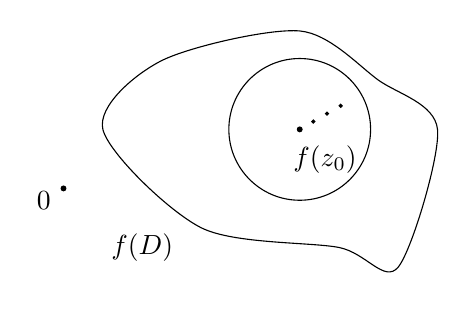
\begin{tikzpicture}
    \draw[scale =0.25]
        plot [smooth cycle] coordinates {(-10,0) (-7,3.5) (0,5)  (4,2.5) (7,0)  (5,-7) (2,-6)  (-5,-5) };


\draw[fill] (0,0) circle (0.03);
\draw (-50:0.5) node {$f(z_0)$};

\draw (0,0) circle (0.9);

\draw[fill] (30:0.2) circle (0.02);
\draw[fill] (30:0.4) circle (0.02);
\draw[fill] (30:0.6) circle (0.02);

\draw node at (-2,-1.5) {$f(D)$};
\draw[fill] (-3,-0.75) circle (0.03);
\draw node at (-3.25,-0.9) {$0$};
\end{tikzpicture}
\end{center}

Since $f(D)$ is open, we can find some sequence $ \{ z_i \} \in D, \, z_i \to z_0 $ s.t. $\abs{f(z_i)} > \abs{f(z_0)}$. Since we can find such a sequence, $z_0$ is not a maximum.
\end{proof}

\begin{corollary}[Maximum Modulus Principle v2]\label{cor:max-mod-prin2}
$\oic$ open, bounded, and connected, $\foc$ holomorphic and continuous up to $\partial \om$ (ie continuous on $\overline{\om}$). Then:
\begin{align*}
    \sup_{\om} \abs{f} = \sup_{\partial \om} \abs{f} < \infty.
\end{align*}
\end{corollary}
\begin{note}
The boundedness and continuity up to $\partial \om$ tells us that $\sup_{\om} \abs{f} = \sup_{\overline{\om}}\abs{f}$ which is finite as the sup over a compact set. For the same reason the RHS is also finite.
\end{note}

\begin{proof}
By assumption, $\sup_{\overline{\om}} \abs{f} < \infty$. Since $f$ is continuous up to $\partial \om$, $\sup_{\overline{\om}} \abs{f} = \sup_{\om} \abs{f}$ (this is since any point in $\overline{\om}$ is a limit of some sequence inside $\om$, and the continuity of $f$ ensures that $\lim f(x_i) = f(\lim x_i)$). Clearly $\sup_{\overline{\om}} \abs{f} \geq \sup_{\partial \om} \abs{f}$, since $\overline{\om} \supset \partial \om$. It thus suffices to show that $\sup_{\om} \abs{f} \leq \sup_{\partial \om} \abs{f}$.

If this is false then
\begin{align}\label{eq:max-mod-prin2-proof}
    \sup_{\om} \abs{f} > \sup_{\partial \om} \abs{f}.
\end{align}
Then let $x \in \overline{\om}$ where $\sup_{\overline{ \om}} \abs{f} $ is achieved (it is achieved since $\overline{\om}$ is compact). By (\ref{eq:max-mod-prin2-proof}), $x \in \om$, hence $\abs{f}$ has a global maximum in $\om$ and is thus constant by corollary (\ref{cor:max-mod-prin1}), an absurdity since for a constant function (\ref{eq:max-mod-prin2-proof}) makes no sense.
\end{proof}
















































































%FILL IN THE RIGHT INFO.
%\lecture{**LECTURE-NUMBER**}{**DATE**}
\unchapter{Lecture 13}
\lecture{13}{October 15}
\setcounter{section}{0}
\setcounter{theorem}{0}

% **** YOUR NOTES GO HERE:

Recall from last lecture the Maximum Modulus Principle v2 (12.16). In the assumption, we require that $\om$ is bounded. We will provide an example where the Maximum Modulus Principle v2 does not hold when $\om$ is unbounded.

\section{Applications of MMP}

\begin{example}

Take $\om = \text{quarter plane} = \set{ z \in \C \mid \Re (z),\Im(z)  > 0 }$. Then $\partial \om = \set{z \in \C \mid \Re(z) = 0 \lor \Im(z) = 0}$.



\begin{center}
\begin{tikzpicture}[very thick,decoration={
    markings,
    mark=at position 0.5 with {\arrow{>}}}
    ]
    
    \draw [thin] (-1,0)--(3,0);
    \draw [thin] (0,-1)--(0,3);
    
    \fill [pattern=north west lines] (0,0) rectangle (3,3);
    
    \draw [very thick] (3,0) -- (0,0) -- (0,3);
    \draw [right](3,2) node {$\om$};
    \draw [below](1,0) node {$\partial \om$};
    
\end{tikzpicture}
\end{center}




Let $F(z) = e^{-iz^2}$ (holomorphic on $\C$ thus on $\om$ as well). It is easy to check that $z \in \partial \om \implies \abs{F(z)} = 1$. But letting $z = re^{\frac{i \pi}{4}} \in \om \implies \abs{F(z)} = e^{r^2}$ which is unbounded (in particular this is larger than $1$). Thus the Maximum Modulus Principle v2 fails.

\end{example}

\begin{example}
Say $D= D_1(0)$, $f: \overline{D} \to \C$ holomorphic non-constant s.t. $\abs{f(z)} \leq 1 \; \forall z \in \partial D$. We will show that $f(D) \subset D$.\\

By the Maximum Modulus Principle v2, $\sup_{D} \abs{f} = \sup_{\partial D} \abs{f} \leq 1$. Then $f(D) \subset \overline{D}$.\\

To prove that $f(D) \subset D$, let us use Maximum Modulus Principle v1: if this fails, then $\exists z_0 \in D$ s.t. $\abs{f(z_0)} = 1$, thus $\abs{f}$ achieves a max at $z_0$ and must be constant.
\end{example}


\section{Automorphisms}

\begin{theorem}
Let $\oic$ open, $\foc$ holomorphic and injective. Then:

\begin{enumerate}
    \item $f(\om)$ is open
    \item $f:\om \to f(\om)$ is bijective
    \item $f'(z) \neq 0 \; \; \forall z \in \om$
    \item $f^{-1}: f(\om) \to \om$ is holomorphic
\end{enumerate}

\end{theorem}

\begin{note}
This does not hold in the real case. Compare point 3 with the function $f(x) = x^3$. This is a smooth injective function from $\R$ to $\R$, but its derivative vanishes at the origin.
\end{note}


\begin{proof}
\begin{enumerate}
    \item $f$ injective $\implies$ $f$ non-constant $\implies$ $f$ open map. Thus $f(\om)$ is open.
    \item $f$ is injective, so obviously bijective.
    \item $f' \nequiv 0$ on $\om$ (if it was, $f$ would be locally constant and thus not injective). Thus since $f'$ is holomorphic and $f' \nequiv 0$, the zeroes of $f$ are isolated. Let us show that $f'$ is never $0$.\\
    
    Suppose that $\exists \, z_0$ s.t. $f'(z_0) = 0$. Let $w_0 = f(z_0)$ and Let $F(z) = f(z) - w_0$. Then $F$ has an isolated zero at $z_0$ (if not isolated, $f \equiv w_0 \; \lightning$). We have that $F'(z_0) = f'(z_0) = 0$, so $z_0$ is a zero of $F$ of order $N \geq 2$. For $z$ close to $z_0$, $F'(z) \neq 0$.\\
    
    We argue exactly the same as in the proof of the Open Mapping Theorem (12.13) and get that (using Rouché) for $w$ close to $w_0$, $f(z) = w$ has exactly $N$ solutions close to $z_0$. But at all such $z$, $f'(z) \neq 0$, so these are all distinct (since if two coincide, $f$ at that point has a zero of order at least two, thus $f'$ at that point is 0). Since $N\geq 2$, we get that $f$ is not injective (since there are at least two distinct zeroes of $f(z) - w$, thus two points that are mapped to $w$).\\
    
    Hence $f'$ never vanishes on $\om$.
    \item To show that $f^{-1}$ is holomorphic, for any $w_0 \in f(\om)$, write $w_0 = f(z_0)$ (uniquely) and for $w$ near $w_0$, write $w = f(z)$ (uniquely). Then, noting that since $z,z_0$ are unique and since $f^{-1}$ is continuous, then as $w \to w_0$, $z \to z_0$:
    
    \begin{align*}
        \lim_{w \to w_0}\frac{f^{-1} (w) - f^{-1} (w_0)  }{w-w_0} &= \lim_{z \to z_0} \frac{z-z_0}{f(z) - f(z_0)}\\
        &= \lim_{z \to z_0} \frac{1}{\frac{f(z) - f(z_0)}{z-z_0}}\\
        &= \frac{1}{f'(z_0)}
    \end{align*}
    
    Since this limit exists, $f^{-1}$ is holomorphic.
\end{enumerate}
\end{proof}

\begin{definition}[Automorphism]
An \textbf{automorphism of $\om$} is a function $f: \om \to \om \subset \C$ open, $f$ holomorphic bijection. Note that by the theorem above, $f^{-1}$ is holomorphic and bijective from $\om $ to $\om$.
\end{definition}

\begin{definition}[Automorphism Group]
We define:
\begin{align*}
Aut(\om) \vcentcolon = \set{f:\om \to \om \mid f \text{ automorphism of } \om}
\end{align*}
This is called the \textbf{automorphism group of $\om$}.
\end{definition}

\begin{note}
$Aut(\om)$ has a natural group structure. Indeed:

\begin{itemize}
    \item Identity is: $Id : \om \to \om$
    \item Group law is: $f \cdot g = f \circ g$
    \item Inverse is: $(f)^{-1} = f^{-1}$
\end{itemize}

\end{note}

\begin{example}[$Aut(\C)$]

We showed in homework 5 (Stein-Shakarchi, Exercise 3.14) that $f: \C \to \C $ holomorphic injective $\implies$ $f = az+b, \, a,b \in \C, \, a \neq 0$. The converse is true trivially. Functions of the form $az+b$ are also obviously bijective.\\

We conclude that $Aut(\C) = \set{az+b \mid a,b \in \C, \, a \neq 0}$


\end{example}

\begin{notation}
$\C^* \vcentcolon= \C \setminus \{ 0 \} $
\end{notation}


\begin{example}[$Aut(\C^*)$]

$Aut(\C^*) \vcentcolon = \set{f:\C^* \to \C^* \mid f \text{ holomorphic and bijective} }$.

To calculate $Aut(\C^*)$, let us look near $0$. $0$ is an isolated singularity of $f$, so there are three cases:


\begin{enumerate}
    \item $0$ is a removable singularity
    
    Thus $\exists$ $\Tilde{f}: \C \to \C$ holomorphic s.t. $\Tilde{f} \mid_{\C^*} = f$. We shall show that necessarily $\Tilde{f} (0) =0$.
    
    Suppose that $\Tilde{f} (0) = z \neq 0$. Then since $f$ is bijective $\exists ! \, w \neq 0$ s.t. $f(w) = z = f(0)$. Let $\varepsilon >0$ s.t. $D_\varepsilon(0) \cap D_\varepsilon(w) = \varnothing$. By the open mapping theorem $\Tilde{f} \left( D_\varepsilon(0) \right) $ and $\Tilde{f} \left( D_\varepsilon(w) \right) $ are open, and $z \in \Tilde{f} \left( D_\varepsilon(0) \right) \cap \Tilde{f} \left( D_\varepsilon(w) \right) $. $\Tilde{f} \left( D_\varepsilon(0) \right) \cap \Tilde{f} \left( D_\varepsilon(w) \right) $ is open and non-empty, thus $\exists \Tilde{z} \neq z, \, \Tilde{z} \in \Tilde{f} \left( D_\varepsilon(0) \right) \cap \Tilde{f} \left( D_\varepsilon(w) \right) $. Thus $\exists a \neq 0, \, a \in D_\varepsilon (0)$ and $b \neq 0, \, b \in D_\varepsilon (w)$ with $a \neq b$ s.t. $f(a) = f(b) = \Tilde{z}$. This is in contradiction to the condition that $f$ is injective on $\C ^*$. It follows that $\Tilde{f}(0) = 0$.
    
    
    Thus $\Tilde{f}: \C \to \C$ is bijective.\\
    
    Thus $\Tilde{f} \in Aut(\C)$ with $\Tilde{f} (0) = 0$. It follows that $f(z) = az, \, z \neq 0$. Clearly $f(z) = az, \, a \neq 0$ is an automorphism of $\C^*$
    
    \item $0$ is a pole
    
    Let $g(z) = \frac{1}{f(z)}$. $g(z):\C^* \to \C^* $ is also bijective and holomorphic as a composition of two holomorphic bijections. Thus $g(z) \in Aut(\C^*)$, but since $0$ is a pole of $f$, $0$ is a removable singularity of $g$.\\
    
    By case 1, $g(z) = az, \, a \neq 0$. It follows that $f(z) = \frac{1}{az}, \, a \neq 0$. Clearly \\ $f(z) = \frac{1}{az}, \, a \neq 0$ is an automorphism of $\C ^*$.
    
    \item $0$ is a n essential singularity
    
    This cannot be. This can be seen by applying Caosrati-Weierstra{\ss} and the Open Mapping Theorem to an open neighborhood around $0$.
    
\end{enumerate}

It follows that $Aut(\C^*) = \set{ f(z) = az \text{ or } \frac{1}{az}, \, a \neq 0}$


\end{example}


Much later we will discuss $Aut(D)$, $Aut(D^*)$, and $Aut(\mathbb{H})$ where $\mathbb{H}$ is the upper half plane


\section{Riemann Sphere}

We turn our attention now to a topic quite different from what we have seen before. We want to be able to describe the relationship between a sphere and the complex plane. Intuitively, we would like to take the $1$-point compactification $\C \sqcup \{ \infty \} = S^2$ sphere.





\begin{center}
    
\begin{tikzpicture}[scale=0.5] % CENT

\def\R{2.5} % sphere radius
\def\angEl{15} % elevation angle
\def\angAz{-10} % azimuth angle
\def\angPhi{-40} % longitude of point P
\def\angBeta{180-25} % latitude of point P

%% working planes

\pgfmathsetmacro\H{\R*cos(\angEl)} % distance to north pole
\tikzset{xyplane/.style={cm={cos(\angAz),sin(\angAz)*sin(\angEl),-sin(\angAz),
                              cos(\angAz)*sin(\angEl),(0,0)}}}
%\tikzset{xyplane/.style={cm={cos(\angAz),sin(\angAz)*sin(\angEl),-sin(\angAz),
%                              cos(\angAz)*sin(\angEl),(0,-\H)}}}
\LongitudePlane[xzplane]{\angEl}{\angAz}
\LongitudePlane[pzplane]{\angEl}{\angPhi}
\LatitudePlane[equator]{\angEl}{0}

\draw [xyplane] (-2.5*\R,-2*\R) rectangle (2*\R,2*\R);
\coordinate[mark coordinate] (N) at (0,\H);
\coordinate[mark coordinate] (S) at (0,-\H);

\draw (N) +(-0.3ex,0.6ex) node[above right] {$\infty$};
\draw (S) +(-0.4ex,-0.4ex) node[below] {\phantom{}};
\draw [white][fill=white] (S) circle (0.1);

\draw (0,0) node {$\C$};


\end{tikzpicture}
\begin{tikzpicture}
\draw (0,1.5) node {  $\xleftrightarrow[]{\phantom{sentence}}$};
\draw (0,0) node {} ;
\end{tikzpicture}
\begin{tikzpicture}[scale=0.5] % CENT





\def\R{2.5} % sphere radius
\def\angEl{15} % elevation angle
\def\angAz{-10} % azimuth angle
\def\angPhi{-40} % longitude of point P
\def\angBeta{180-25} % latitude of point P

%% working planes

\pgfmathsetmacro\H{\R*cos(\angEl)} % distance to north pole
\tikzset{xyplane/.style={cm={cos(\angAz),sin(\angAz)*sin(\angEl),-sin(\angAz),
                              cos(\angAz)*sin(\angEl),(0,0)}}}
%\tikzset{xyplane/.style={cm={cos(\angAz),sin(\angAz)*sin(\angEl),-sin(\angAz),
%                              cos(\angAz)*sin(\angEl),(0,-\H)}}}
\LongitudePlane[xzplane]{\angEl}{\angAz}
\LongitudePlane[pzplane]{\angEl}{\angPhi}
\LatitudePlane[equator]{\angEl}{0}

%% draw xyplane and sphere

%\draw[xyplane] (-2*\R,-2*\R) rectangle (2.2*\R,2.8*\R);
\draw (0,0) circle (\R);

%% characteristic points

\coordinate (O) at (0,0);

\draw [xyplane] (-2.5*\R,-2*\R) rectangle (2*\R,2*\R);
\coordinate[mark coordinate] (N) at (0,\H);
                                        
%\coordinate[mark coordinate] (Phat2) at (intersection cs: first line={(S)--(P)},
%                                        second line={(0,0)--(Paux)});

%% draw meridians and latitude circles

\DrawLatitudeCircle[\R]{0} % equator





%% draw lines and put labels

\draw (N) +(-0.3ex,0.6ex) node[above right] {$\infty = \text{North Pole}$};

%\draw (Phat2) node[above right] {$\mathbf{R}$};




\end{tikzpicture}
\end{center}























\subsection{Stereographic Projection}


Consider a sphere intersected with a plane. Then given any point $P \in S^2\setminus \{ N \}$ there is a unique line containing $P$ and $N$. This line intersects the $xy$-plane in a point $Q$.













\begin{center}
    
\begin{tikzpicture} % CENT

%% some definitions

\def\R{2.5} % sphere radius
\def\angEl{15} % elevation angle
\def\angAz{-10} % azimuth angle
\def\angPhi{-40} % longitude of point P
\def\angBeta{180-25} % latitude of point P

%% working planes

\pgfmathsetmacro\H{\R*cos(\angEl)} % distance to north pole
\tikzset{xyplane/.style={cm={cos(\angAz),sin(\angAz)*sin(\angEl),-sin(\angAz),
                              cos(\angAz)*sin(\angEl),(0,0)}}}
%\tikzset{xyplane/.style={cm={cos(\angAz),sin(\angAz)*sin(\angEl),-sin(\angAz),
%                              cos(\angAz)*sin(\angEl),(0,-\H)}}}
\LongitudePlane[xzplane]{\angEl}{\angAz}
\LongitudePlane[pzplane]{\angEl}{\angPhi}
\LatitudePlane[equator]{\angEl}{0}

%% draw xyplane and sphere

%\draw[xyplane] (-2*\R,-2*\R) rectangle (2.2*\R,2.8*\R);
\draw (0,0) circle (\R);

%% characteristic points

\coordinate (O) at (0,0);

\draw [xyplane] (-2.5*\R,-2*\R) rectangle (2*\R,2*\R);
\coordinate[mark coordinate] (N) at (0,\H);
\coordinate[mark coordinate] (S) at (0,-\H);
\path[pzplane] (\angBeta:\R) coordinate[mark coordinate] (P);
\path[pzplane] (\R,0) coordinate (PE);
\path[xzplane] (\R,0) coordinate (XE);
\path (PE) ++(0,0) coordinate (Paux); % to aid Phat calculation
%\path (PE) ++(0,-\H) coordinate (Paux); % to aid Phat calculation
\coordinate[mark coordinate] (Phat) at (intersection cs: first line={(N)--(P)},
                                        second line={(0,0)--(Paux)});
                                        
%\coordinate[mark coordinate] (Phat2) at (intersection cs: first line={(S)--(P)},
%                                        second line={(0,0)--(Paux)});

%% draw meridians and latitude circles

\DrawLatitudeCircle[\R]{0} % equator





%% draw lines and put labels

\draw (P) -- (N) +(-0.3ex,0.6ex) node[above right] {$\mathbf{N}$};

\draw (S) +(-0.4ex,-0.4ex) node[below] {$\mathbf{S}$};

\draw (P) -- (Phat) node[above left] {$\mathbf{Q}$};
\draw (P) node[above left] {$\mathbf{P}$};
%\draw (Phat2) node[above right] {$\mathbf{R}$};




\end{tikzpicture}
\end{center}























\begin{definition}

The map that takes $P$ to $Q$ is called the \textbf{stereographic projection from $N$}, denoted by $Str_N$.
\end{definition}


\begin{remark}
This is a bijection between $S^2 \setminus \{ N \}$ and $\R^2 = \C$.
\end{remark}

Now taking the stereographic projection from $S$ gives you a different bijection between $S^2 \setminus \{ S \}$ and $\R^2 = \C$ that takes $P$ to some point $R \in \R^2$.


\begin{center}
    
\begin{tikzpicture} % CENT

%% some definitions

\def\R{2.5} % sphere radius
\def\angEl{15} % elevation angle
\def\angAz{-10} % azimuth angle
\def\angPhi{-40} % longitude of point P
\def\angBeta{180-25} % latitude of point P

%% working planes

\pgfmathsetmacro\H{\R*cos(\angEl)} % distance to north pole
\tikzset{xyplane/.style={cm={cos(\angAz),sin(\angAz)*sin(\angEl),-sin(\angAz),
                              cos(\angAz)*sin(\angEl),(0,0)}}}
%\tikzset{xyplane/.style={cm={cos(\angAz),sin(\angAz)*sin(\angEl),-sin(\angAz),
%                              cos(\angAz)*sin(\angEl),(0,-\H)}}}
\LongitudePlane[xzplane]{\angEl}{\angAz}
\LongitudePlane[pzplane]{\angEl}{\angPhi}
\LatitudePlane[equator]{\angEl}{0}

%% draw xyplane and sphere

%\draw[xyplane] (-2*\R,-2*\R) rectangle (2.2*\R,2.8*\R);
\draw (0,0) circle (\R);

%% characteristic points

\coordinate (O) at (0,0);

\draw [xyplane] (-2.5*\R,-2*\R) rectangle (2*\R,2*\R);
\coordinate[mark coordinate] (N) at (0,\H);
\coordinate[mark coordinate] (S) at (0,-\H);
\path[pzplane] (\angBeta:\R) coordinate[mark coordinate] (P);
\path[pzplane] (\R,0) coordinate (PE);
\path[xzplane] (\R,0) coordinate (XE);
\path (PE) ++(0,0) coordinate (Paux); % to aid Phat calculation
%\path (PE) ++(0,-\H) coordinate (Paux); % to aid Phat calculation
\coordinate[mark coordinate] (Phat) at (intersection cs: first line={(N)--(P)},
                                        second line={(0,0)--(Paux)});
                                        
\coordinate[mark coordinate] (Phat2) at (intersection cs: first line={(S)--(P)},
                                        second line={(0,0)--(Paux)});

%% draw meridians and latitude circles

\DrawLatitudeCircle[\R]{0} % equator





%% draw lines and put labels

\draw (P) -- (N) +(-0.3ex,0.6ex) node[above right] {$\mathbf{N}$};

\draw (P) -- (S) +(-0.4ex,-0.4ex) node[below] {$\mathbf{S}$};

\draw (P) -- (Phat) node[above left] {$\mathbf{Q}$};
\draw (P) node[above left] {$\mathbf{P}$};
\draw (Phat2) node[above right] {$\mathbf{R}$};




\end{tikzpicture}
\end{center}















We want to find a map $\phi : \C \to \C$, $Q \mapsto R$. Consider $Q = (x,y,0)$ and $N= (0,0,1)$. To find $P $ we parameterize $\overline{QN}$ by $t \cdot (0,0,1) + (1-t) \cdot (x,y,0) = \big( (1-t) \cdot x, \, (1-t) \cdot y, \, t \big) = \gamma(t)$.



\begin{center}
    
\begin{tikzpicture} % CENT

%% some definitions

\def\R{2.5} % sphere radius
\def\angEl{15} % elevation angle
\def\angAz{-10} % azimuth angle
\def\angPhi{-40} % longitude of point P
\def\angBeta{180-25} % latitude of point P

%% working planes

\pgfmathsetmacro\H{\R*cos(\angEl)} % distance to north pole
\tikzset{xyplane/.style={cm={cos(\angAz),sin(\angAz)*sin(\angEl),-sin(\angAz),
                              cos(\angAz)*sin(\angEl),(0,0)}}}
%\tikzset{xyplane/.style={cm={cos(\angAz),sin(\angAz)*sin(\angEl),-sin(\angAz),
%                              cos(\angAz)*sin(\angEl),(0,-\H)}}}
\LongitudePlane[xzplane]{\angEl}{\angAz}
\LongitudePlane[pzplane]{\angEl}{\angPhi}
\LatitudePlane[equator]{\angEl}{0}

%% draw xyplane and sphere

%\draw[xyplane] (-2*\R,-2*\R) rectangle (2.2*\R,2.8*\R);
\draw (0,0) circle (\R);

%% characteristic points

\coordinate (O) at (0,0);

\draw [xyplane] (-2.5*\R,-2*\R) rectangle (2*\R,2*\R);
\coordinate[mark coordinate] (N) at (0,\H);
\coordinate[mark coordinate] (S) at (0,-\H);
\path[pzplane] (\angBeta:\R) coordinate[mark coordinate] (P);
\path[pzplane] (\R,0) coordinate (PE);
\path[xzplane] (\R,0) coordinate (XE);
\path (PE) ++(0,0) coordinate (Paux); % to aid Phat calculation
%\path (PE) ++(0,-\H) coordinate (Paux); % to aid Phat calculation
\coordinate[mark coordinate] (Phat) at (intersection cs: first line={(N)--(P)},
                                        second line={(0,0)--(Paux)});
                                        
\coordinate[mark coordinate] (Phat2) at (intersection cs: first line={(S)--(P)},
                                        second line={(0,0)--(Paux)});

%% draw meridians and latitude circles

\DrawLatitudeCircle[\R]{0} % equator





%% draw lines and put labels

\draw (P) -- (N) +(-0.3ex,0.6ex) node[above right] {$\mathbf{N=(0,0,1)}$};

\draw (P) -- (S) +(-0.4ex,-0.4ex) node[below] {$\mathbf{S=(0,0,-1)}$};

\draw (P) -- (Phat) node[above left] {$\mathbf{(x,y,0)=Q}$};
\draw (P) node[above left] {$\mathbf{P}$};
\draw (Phat2) node[above right] {$\mathbf{R}$};




\end{tikzpicture}
\end{center}




Now $P$ is (one) intersection of $\gamma$ and $S^2$ such that:

\begin{align*}
    1 = \abs{\gamma(t) }^2 &= (1-t)^2x^2 + (1-t)^2 y^2 + t^2\\
    \text{(letting $A \vcentcolon = x^2 + y^2$) } &= t^2 (A+1) - 2At + A 
\end{align*}

This is quadratic in $t$. Thus:

\begin{align*}
    t &= \frac{A \pm \sqrt{A^2 - (A^2 - 1)}}{A+1}\\ \text{(ignore $t=1$; this is N) } &= \frac{A-1}{A+1}
\end{align*}

Thus, with $(1-t) = \frac{2}{A+1}$:

\begin{align*}
    P &= \bigg( \underbrace{\frac{2x}{x^2+y^2+1} }_{\mathfrak{X}}, \,  \underbrace{\frac{2y}{x^2+y^2+1}}_{\mathfrak{Y}} , \, \underbrace{\frac{x^2+y^2-1}{x^2+y^2+1}}_{\mathfrak{Z}}  \bigg)\\
    &= \left( \mathfrak{X}, \, \mathfrak{Y}, \, \mathfrak{Z} \right)
\end{align*}

Now take $\Tilde{\gamma} = \overline{SP} = \big( (1-t) \cdot \mathfrak{X}, \, (1-t) \cdot \mathfrak{Y}, \, (1-t)\cdot \mathfrak{Z} - t \big)$. $R$ is the intersection of $\Tilde{\gamma}$ and the $xy$-plane. Thus $t = \frac{\mathfrak{Z}}{\mathfrak{Z}+1}$ and $1-t = \frac{1}{\mathfrak{Z} + 1}$. It follows (after some arithmetic) that:


\begin{align*}
    R &= \left( \frac{\mathfrak{X}}{\mathfrak{Z} + 1} , \, \frac{\mathfrak{Y}}{\mathfrak{Z}+1} , \, 0 \right) = \left( \frac{x}{x^2+y^2} , \, \frac{y}{x^2+y^2} , \, 0         \right)
\end{align*}


So $\phi = Str_S \circ (Str_N)^{-1}$ maps $Q = (x,y,0)$ to $R = \left( \frac{x}{x^2+y^2} , \, \frac{y}{x^2+y^2} , \, 0         \right)$.

We can think of $Q,R$ as elements of $\R^2 = \C$:

\begin{align*}
    Q &= z = x+iy\\
    R &= \frac{x}{x^2 + y^2} + i \frac{y}{x^2 + y^2}\\
    &= \frac{z}{x^2 + y^2}\\
    &= \frac{z}{\abs{z}^2}\\ &= \frac{1}{\overline{z}}
\end{align*}

%Thus our map is $\phi: \C \to \C$, $z \mapsto \frac{1}{\overline{z}}$ .


If we compose one of the two projections with $\overline{z}$, we get that to obtain $S^2$ you can take two copies of $\C$ and glue them on $\C^* \subset \C$ via the map $z \mapsto \frac{1}{z}$.

ELABORATE
ADD TIKZ

\begin{remark}

This is an atlas with two charts for the $2$-dimensional  manifold $S^2$, where $z \xleftrightarrow[]{} \frac{1}{z}$ is the transition between the two charts.
\end{remark}


We can use this to define holomorphic functions to and from $S^2$.


\begin{definition}

Consider $f: S^2 \to \C$ a map of sets. $f$ is called \textbf{holomorphic} if on $U_1$, $f \circ Str_N: \C \to \C$ is holomorphic and on $U_2$, $f \circ Str_S: \C \to \C$ is holomorphic.
\end{definition}



























%FILL IN THE RIGHT INFO.
%\lecture{**LECTURE-NUMBER**}{**DATE**}
\unchapter{Lecture 14}
\lecture{14}{October 20}
\setcounter{section}{0}
\setcounter{theorem}{0}

% **** YOUR NOTES GO HERE:

\section{Riemann Sphere Continued}

Let $S^2 = \set{ (\mathfrak{X}, \mathfrak{Y}, \mathfrak{Z}) \mid \mathfrak{X}^2 + \mathfrak{Y}^2 +\mathfrak{Z}^2  =1 } \subset \R^3$ be the unit sphere centered at $0$. Last lecture we talked about the stereographic projection from $N = (0,0,1)$ and $S = (0,0,-1)$. Let $U_1 = S^2 \setminus \{ (0,0,1) \}$ and $U_2 = S^2 \setminus \{ (0,0,-1) \}$. These are both open subsets of $S^2$.



\begin{center}
    
\begin{tikzpicture}[scale=0.5] % CENT

%% some definitions

\def\R{2.5} % sphere radius
\def\angEl{15} % elevation angle
\def\angAz{-10} % azimuth angle
\def\angPhi{-40} % longitude of point P
\def\angBeta{180-25} % latitude of point P

%% working planes

\pgfmathsetmacro\H{\R*cos(\angEl)} % distance to north pole
\tikzset{xyplane/.style={cm={cos(\angAz),sin(\angAz)*sin(\angEl),-sin(\angAz),
                              cos(\angAz)*sin(\angEl),(0,0)}}}
%\tikzset{xyplane/.style={cm={cos(\angAz),sin(\angAz)*sin(\angEl),-sin(\angAz),
%                              cos(\angAz)*sin(\angEl),(0,-\H)}}}
\LongitudePlane[xzplane]{\angEl}{\angAz}
\LongitudePlane[pzplane]{\angEl}{\angPhi}
\LatitudePlane[equator]{\angEl}{0}

%% draw xyplane and sphere

%\draw[xyplane] (-2*\R,-2*\R) rectangle (2.2*\R,2.8*\R);
\draw (0,0) circle (\R);

%% characteristic points

\coordinate (O) at (0,0);

\draw [xyplane] (-2.5*\R,-2*\R) rectangle (2*\R,2*\R);
\coordinate[mark coordinate] (N) at (0,\H);
\coordinate[mark coordinate] (S) at (0,-\H);
\path[pzplane] (\angBeta:\R) coordinate[mark coordinate] (P);
\path[pzplane] (\R,0) coordinate (PE);
\path[xzplane] (\R,0) coordinate (XE);
\path (PE) ++(0,0) coordinate (Paux); % to aid Phat calculation
%\path (PE) ++(0,-\H) coordinate (Paux); % to aid Phat calculation
\coordinate[mark coordinate] (Phat) at (intersection cs: first line={(N)--(P)},
                                        second line={(0,0)--(Paux)});
                                        
\coordinate[mark coordinate] (Phat2) at (intersection cs: first line={(S)--(P)},
                                        second line={(0,0)--(Paux)});

%% draw meridians and latitude circles

\DrawLatitudeCircle[\R]{0} % equator





%% draw lines and put labels

\draw (P) -- (N) +(-0.3ex,0.6ex) node[above right] {$\mathbf{N=(0,0,1)}$};

\draw (P) -- (S) +(-0.4ex,-0.4ex) node[below] {$\mathbf{S=(0,0,-1)}$};

\draw (P) -- (Phat) node[above left] {$\mathbf{(x,y,0)=Q}$};
\draw (P) node[above left] {$\mathbf{P}$};
\draw (Phat2) node[above right] {$\mathbf{R}$};




\end{tikzpicture}
\end{center}





Define $\phi_1:U_1 \to \C, \, P \mapsto Q$ to be the stereographic projection from $N$. We showed last time that:
\begin{align*}
\phi_1 (\mathfrak{X}, \mathfrak{Y}, \mathfrak{Z}) &= \frac{\mathfrak{X}}{1 - \mathfrak{Z}} + i \frac{ \mathfrak{Y}}{1 - \mathfrak{Z}}.\\
\phi_1^{-1} (x+iy) &= \bigg( \frac{2x}{x^2+y^2+1} , \,  \frac{2y}{x^2+y^2+1} , \, \frac{x^2+y^2-1}{x^2+y^2+1}  \bigg).
\end{align*}


Define $\phi_2:U_2 \to \C, \, P \mapsto \overline{R}$ to be the stereographic projection from $S$ composed with complex conjugation. Then:
\begin{align*}
\phi_2 (\mathfrak{X}, \mathfrak{Y}, \mathfrak{Z}) &= \frac{\mathfrak{X}}{1 + \mathfrak{Z}} - i \frac{ \mathfrak{Y}}{1 + \mathfrak{Z}}.
\end{align*}

$U_1 \cap U_2 = S^2 \setminus \set{N,S}$. It is clear that $\phi_1 (U_1 \cap U_2) = \phi_2(U_1 \cap U_2) = \C^*$. We showed in the last lecture that:
\begin{align*}
    \phi_2 \circ \phi_1^{-1} : \, \, \C^* &\to \C^*,\\
    z &\mapsto \frac{1}{z}.
\end{align*}

\begin{note}[If you know about manifolds already]
$\set{ (U_1, \phi_1) , (U_2, \phi_2) }$ is an atlas for $S^2$ as a Riemann surface, since $ \phi_2 \circ \phi_1^{-1} (z) = \frac{1}{z}$ is holomorphic.
\end{note}


\subsection{Holomorphic Maps on $S^2$}
We now want to define the concept of holomorphic maps from and to $S^2$.

\begin{definition}[Holomorphic Functions from $S^2$ to $\C$]

$\om \in S^2$ open (can be $S^2$ itself). Let $\foc$ a map of sets. We say that \textbf{$f$ is holomorphic} if on $\phi_1 ( U_1 \cap \om) \subset \C$ open, $F_1 \vcentcolon= f \circ \phi_1^{-1} : \phi_1(U_1 \cap \om) \to \C$ is holomorphic and if on $\phi_2 ( U_2 \cap \om) \subset \C$ open, $F_2 \vcentcolon= f \circ \phi_2^{-1} : \phi_2(U_2 \cap \om) \to \C$ is holomorphic.\\

Equivalently, $f$ is holomorphic if I have $F_1$ holomorphic on $\Tilde{\om} \subset \C$ holomorphic and $F_2 = f \circ \phi_2^{-1} = F \circ \phi_1 \circ \phi_2^{-1} = F \left( \frac{1}{z} \right)$ is holomorphic near $0$ (if $\Tilde{\om}$ contains a neighborhood of $\infty$).
\end{definition}


\begin{center}
    
\begin{tikzpicture}[scale=1] % CENT

\def\R{1} % sphere radius
\def\angEl{25} % elevation angle
%\def\angEl{15} % elevation angle
\def\angAz{-10} % azimuth angle
%\def\angAz{-10} % azimuth angle

\tikzset{xyplane/.style={cm={cos(\angAz),sin(\angAz)*sin(\angEl),-sin(\angAz), cos(\angAz) *sin(\angEl),(0,0)}}}

\LongitudePlane[xzplane]{\angEl}{\angAz}



% \draw[xyplane] (-2,-2) rectangle (2,2);
% \draw[xyplane] node at (0,0) {$\times$};



\pgfmathsetmacro\H{1.5*cos(\angEl)}


\draw (0,0) circle (1.5);
\DrawLatitudeCircle[1.5]{0} % equator

\draw (0,\H) node {$\times$};
\draw (0,-\H) node {$\times$};


%top right
\draw[xyplane] (-2+8,-2) rectangle (2+8,2);
%\draw[xyplane] node at (8,0) {$\times$};
%bottom left
\draw[xyplane] (-2,-2 -8) rectangle (2,2-8);
\draw[xyplane] node at (0,-8) {$\times$};
%bottom right
\draw[xyplane] (-2+8,-2 -8) rectangle (2+8,2-8);
\draw[xyplane] node at (0+8,-8) {$\times$};



%from sphere
\draw[xyplane][->] (0+2,0) -- (8-2-0.5,0);
\draw[xyplane][->] (0,0-2) -- (0,-8+2+0.5);

%from bottom left
\draw[xyplane][<->] (0+2+0.5,0-8) -- (8-2-0.5,0-8);


%from bottom right
\draw[xyplane][->] (8,-8+2+0.5) -- (8,0-2-0.5);



%across middle
% \draw[xyplane][->] (0+2,0-2) -- (8-2,-8+2);
% \draw[xyplane][->] (0+2,0-8+2) -- (8-2,0-2);

\draw[xyplane][->] ($ (8,0)+(225:8) $) -- ($ (0,-8)+(45:8) $);
\draw[xyplane][color = white][fill = white] (4,-4) circle (0.25);

\draw[xyplane][->] (-45:2.8) -- (-45:8);



\draw[xyplane][above] node at (4,0) {$f$};
\draw[xyplane][above] node at (4,-8) {$z \mapsto \frac{1}{z}$};

\draw[xyplane][right] node at (0,-4.75) {$\phi_1$};
\draw[xyplane][above right] node at (-45:7) {$\phi_2$};
\draw[xyplane][right] node at (8,-3.75) {$F_2$};
\draw[xyplane][above left] node at ($ (0,-8)+(45:7) $) {$F_1$};

\draw[xyplane][below right] node at (8+2,-1.5) {$\mathbb{C}$};
\end{tikzpicture}

\end{center}

% \begin{tikzpicture}
% for i in range [0,30, 60 , ... , 6000]
% \draw circle($1/i$) at 0;
% \end{tikzpicture}


\begin{definition}[Holomorphic Functions from $\C$ to $S^2$]

If $\oic$ open, $f: \om \to S^2$ a map of sets, we say that \textbf{$f$ is holomorphic} if both $\phi_1 \circ f: \om \to \C$ and $\phi_2 \circ f: \om \to \C$ are holomorphic.\\

Equivalently, $F = \phi_1 \circ f$ holomorphic and $\phi_2 \circ f = \phi_2 \circ \phi_1^{-1} \circ F = \frac{1}{F}$ holomorphic on $\om \cap \set{F \neq 0}$ ie $F$ has only poles, where $poles = f^{-1} (\text{north pole})  =f^{-1} ( `` \infty" )$.






















\begin{center}
    
\begin{tikzpicture}[scale=1] % CENT

\def\R{1} % sphere radius
\def\angEl{25} % elevation angle
%\def\angEl{15} % elevation angle
\def\angAz{-10} % azimuth angle
%\def\angAz{-10} % azimuth angle

\tikzset{xyplane/.style={cm={cos(\angAz),sin(\angAz)*sin(\angEl),-sin(\angAz), cos(\angAz) *sin(\angEl),(0,0)}}}

\LongitudePlane[xzplane]{\angEl}{\angAz}



% \draw[xyplane] (-2,-2) rectangle (2,2);
% \draw[xyplane] node at (0,0) {$\times$};



\pgfmathsetmacro\H{1.5*cos(\angEl)}


\draw (0,0) circle (1.5);
\DrawLatitudeCircle[1.5]{0} % equator

\draw (0,\H) node {$\times$};
\draw (0,-\H) node {$\times$};


%left
\draw[xyplane] (-2-8,-2) rectangle (2-8,2);
%\draw[xyplane] node at (-8,0) {$\times$};
%bottom
\draw[xyplane] (-2-4,-2 -8) rectangle (2-4,2-8);
%\draw[xyplane] node at (0,-8) {$\times$};
%top
\draw[xyplane] (-2-4,-2 +8) rectangle (2-4,2+8);
%\draw[xyplane] node at (0-4,8) {$\times$};



%from left
\draw[xyplane][->]  (-8+2+0.5,0) -- (0-2,0);
\draw[xyplane][->] (-8+1.5,-2-0.5) -- (-5.5,-8+2+0.5);
\draw[xyplane][->] (-8+1.5,2+0.5) -- (-5.5,+8-2-0.5);

%from sphere
\draw[xyplane][->] (-110:2) -- (-2.5,-8+2+0.5);
\draw[xyplane][->] (110:2) -- (-2.5,+8-2-0.5);





\draw[xyplane][above right] node at ($ (110:1) + (-2.5/2,5.5/2) $) {$\phi_1$};
\draw[xyplane][below right] node at ($ (-110:1) + (-2.5/2,-5.5/2) $) {$\phi_2$};

\draw[xyplane][above left] node at ($ (-6.5/2,+2.5/2) + (-5.5/2,+5.5/2) $) {$\phi_1 \circ f$};
\draw[xyplane][below left] node at ($ (-6.5/2,-2.5/2) + (-5.5/2,-5.5/2) $) {$\phi_2 \circ f$};

\draw[xyplane][above] node at (-4,0) {$f$};
\draw[above right] node at (50:1.5) {$S^2$};


\draw[xyplane][below right] node at (-8+2,-1.5) {$\mathbb{C}$};
\end{tikzpicture}

\end{center}




























\end{definition}

\begin{definition}[Holomorphic Functions from $S^2$ to $S^2$]

$\om \subset S^2$ open, $f:\om \to S^2$ a map of sets. \textbf{$f$ is holomorphic} if:
\begin{align*}
    \phi_1 \circ f \circ \phi_1^{-1} : \phi_1 \left( U_1 \cap U_1 \right) \to \phi_1 \left( U_1 \cap U_1\right),\\
    \phi_1 \circ f \circ \phi_2^{-1} : \phi_2 \left( U_1 \cap U_2 \right) \to \phi_1 \left( U_1 \cap U_2\right),\\
    \phi_2 \circ f \circ \phi_1^{-1} : \phi_1 \left( U_2 \cap U_1 \right) \to \phi_2 \left( U_2 \cap U_1\right),\\
    \phi_2 \circ f \circ \phi_2^{-1} : \phi_2 \left( U_2 \cap U_2 \right) \to \phi_2 \left( U_2 \cap U_2\right),\\
\end{align*}
are all holomorphic.\\

Equivalently, letting $F= \phi_1 \circ f \circ \phi_1^{-1}$ then $f$ holomorphic as a map $S^2 \to S^2$ if:
\begin{itemize}
    \item F holomorphic,
    \item $f:z \mapsto \infty$ then $F$ has a pole at $z$,
    \item $f:\infty \mapsto z$ then $F$ holomorphic at $\infty$,
    \item $f: \infty \mapsto \infty$ then $F$ has a pole at $\infty$.
\end{itemize}
\end{definition}










\begin{center}
    
\begin{tikzpicture}[scale=0.5] % CENT

\def\R{1} % sphere radius
\def\angEl{25} % elevation angle
%\def\angEl{25} % elevation angle
\def\angAz{-10} % azimuth angle
%\def\angAz{-10} % azimuth angle

\tikzset{xyplane/.style={cm={cos(\angAz),sin(\angAz)*sin(\angEl),-sin(\angAz), cos(\angAz) *sin(\angEl),(0,0)}}}

\LongitudePlane[xzplane]{\angEl}{\angAz}



\pgfmathsetmacro\H{1.5*cos(\angEl)}




\draw[xyplane] (-2,-2) rectangle (2,2);

\draw[xyplane] ($ (-2+6,-2) + (0,{-6*sin(\angAz)})$) rectangle ($ (2+6,2) + (0,{-6*sin(\angAz)})$);

\draw[xyplane] ($ (-2+6+8,-2) + (0,{-14*sin(\angAz)})$) rectangle ($ (2+6+8,2) + (0,{-14*sin(\angAz)})$);

\draw[xyplane] ($ (-2+12+8,-2) + (0,{-20*sin(\angAz)})$) rectangle ($ (2+12+8,2) + (0,{-20*sin(\angAz)})$);




\draw[xyplane] node (A) at ($(3,0) + (0,{-3*sin(\angAz)})$) {};
\draw[xyplane] node (B) at ($ (17,0) + (0,{-17*sin(\angAz)})$) {};
\draw node (Ap) at ($ (A) + (0,6) $) {};
\draw node (Bp) at ($ (B) + (0,6) $) {};

\draw[xyplane] node (C) at ($ (0,0) + (0,{-0*sin(\angAz)})$) {};
\draw[xyplane] node (D) at ($ (6,0) + (0,{-6*sin(\angAz)})$) {};
\draw[xyplane] node (E) at ($ (14,0) + (0,{-14*sin(\angAz)})$) {};
\draw[xyplane] node (F) at ($ (20,0) + (0,{-20*sin(\angAz)})$) {};

\draw node (Cp) at ($ (C) + (0,1) $) {};
\draw node (Dp) at ($ (D) + (0,1) $) {};
\draw node (Ep) at ($ (E) + (0,1) $) {};
\draw node (Fp) at ($ (F) + (0,1) $) {};



\DrawLatitudeCircleShiftOne[1.5]{0} % equator
\DrawLatitudeCircleShiftTwo[1.5]{0} % equator

\draw (Ap) circle (1.5);
\draw (Bp) circle (1.5);


\draw [->] ($ (Ap) + (0:1.75) $) -- ($ (Bp) + (180:1.75) $) node [midway, above] {$f$};
\draw [->] ($ (Ap) + (-120:1.75)$) -- (Cp);
\draw [->] ($ (Ap) + (-60:1.75)$) -- (Dp);
\draw [->] ($ (Bp) + (-120:1.75)$) -- (Ep);
\draw [->] ($ (Bp) + (-60:1.75)$) -- (Fp);

\draw [left] node at ($ (Ap) + (-120:3) + (-0.2,0) $) {$\phi_1$};
\draw [right] node at ($ (Ap) + (-60:3) + (0.2,0) $) {$\phi_2$};
\draw [left] node at ($ (Bp) + (-120:3) + (-0.2,0) $) {$\phi_1$};
\draw [right] node at ($ (Bp) + (-60:3) + (0.2,0) $) {$\phi_2$};


\end{tikzpicture}

\end{center}




































\begin{remark}
It follows that $f: S^2 \to S^2$ holomorphic $\iff$ $F=\phi_1 \circ f \circ \phi_1^{-1}$ meromorphic in $\C$ and meromorphic at $\infty$. By theorem (\ref{thm:char-rat}) this is equivalent to $F$ being a rational function ie $F$ is the ratio of two complex polynomials.
\end{remark}

\begin{exercise}
Compute $Aut(S^2)$. That is to say, characterize the bijective holomorphic maps from $S^2 $ to $S^2$.
\end{exercise}



\section{Homotopy and Contour Integrals}

Homotopies are often discussed in an introduction to algebraic topology. We will give a simple-minded yet perfectly rigorous introduction to homotopies.\\

A homotopy is in a sense a ``continuous family of continuous paths." This must be defined, but in our treatment we will insist on having piecewise smooth paths. Say $\gamma_0, \gamma_1$ are two piecewise smooth curves in $
C$. Up to reparameterization we may assume that both are parameterized by the same interval $t \in [a,b] \subset \R$. Assume that $\gamma_0(a) = \gamma_1(a) = z_0$ and $\gamma_0(b) = \gamma_1(b) = z_1$.

\begin{center}
\begin{tikzpicture}[decoration={
    markings,
    mark=at position 0.6 with {\arrow{>}}}
    ]
    \node[label={[above left] $z_0$}] (a3) at (0,0) {};
    \node[label={[above right]$z_1$}] (b3) at (10,0) {};
    \draw[fill] (a3) circle (0.08);
    \draw[fill] (b3) circle (0.08);
    \draw[postaction={decorate}][thick] (a3) to[out=50,in=150]node[above]{$\gamma_1$} (b3);
    % \foreach \o/\i in {40/160,30/170,20/180,10/190,-10/200}
       % \draw (a3) to[out=\o,in=\i]  (b3);
    \draw[postaction={decorate}][thick] (a3) to[out=-20,in=-130]node[below]{$\gamma_0$} (b3);
\end{tikzpicture}
\end{center}

\begin{definition}
Suppose that $\gamma_0, \gamma_1 \subset \om$ are two such curves. We say that \textbf{$\gamma_0$ and $\gamma_1$ are homotopic in $\om$} if $\exists F : [0,1] \times [a,b] \to \om$ continuous such that:
\begin{enumerate}
    \item $\forall s \in [0,1] , \, \Tilde{\gamma}_s(t) \defas F(s,t)$ is a piecewise smooth curve $\Tilde{\gamma}_s : [a,b] \to \om$,
    \item $\Tilde{\gamma}_0 = F(0,t) \equiv \gamma_0$ and $\Tilde{\gamma}_1 = F(1,t) \equiv \gamma_1$,
    \item $\Tilde{\gamma}_s(a) = z_0$ and $\Tilde{\gamma}_s(b) = z_1$ $\forall s \in [0,1]$.
\end{enumerate}

\begin{center}
\begin{tikzpicture}[decoration={
    markings,
    mark=at position 0.6 with {\arrow{>}}}
    ]
    \node[label={[above left] $z_0$}] (a3) at (0,0) {};
    \node[label={[above right]$z_1$}] (b3) at (10,0) {};
    \draw[fill] (a3) circle (0.08);
    \draw[fill] (b3) circle (0.08);
    \draw[postaction={decorate}][thick] (a3) to[out=50,in=150]node[above]{$\gamma_1$} (b3);
    \foreach \o/\i in {40/160,30/170,10/190,-10/200,-15/210}
       \draw (a3) to[out=\o,in=\i]  (b3);
    \draw[postaction={decorate}] (a3) to[out=20,in=-180]node[above]{$\gamma_s$} (b3);
    \draw[postaction={decorate}][thick] (a3) to[out=-20,in=-130]node[below]{$\gamma_0$} (b3);
\end{tikzpicture}
\end{center}

\end{definition}

We can think of $\Tilde{\gamma}_s$ as an interpolating family of piecewise smooth curves with similar beginning and ending points which ``vary continuously in S", where the ``continuous variation" is encoded in the condition that $F$ is continuous.


\begin{counterexample}[Moral Counterexample]
Let $\om = \C^*$.

\begin{center}
\begin{tikzpicture}[decoration={
    markings,
    mark=at position 0.6 with {\arrow{>}}}
    ]
    \node[label={[above left] $-1$}] (a3) at (0,0) {};
    \node[label={[above right]$1$}] (b3) at (10,0) {};
    \node[label={[above right]$0$}] (c3) at (5,0) {};
    \draw[shift=(0:5)][thick] (-0.1,0.1) -- (0.1,-0.1) (0.1,0.1) -- (-0.1,-0.1);
    \draw[fill] (a3) circle (0.08);
    \draw[fill] (b3) circle (0.08);
    \draw[postaction={decorate}][thick] (a3) to[out=50,in=150]node[above]{$\gamma_1$} (b3);
    % \foreach \o/\i in {40/160,30/170,20/180,10/190,-10/200}
       % \draw (a3) to[out=\o,in=\i]  (b3);
    \draw[postaction={decorate}][thick] (a3) to[out=-20,in=-130]node[below]{$\gamma_0$} (b3);
\end{tikzpicture}
\end{center}

These two curves should not be homotopic in $\om$, since $F$ must map into $\om$.
\end{counterexample}

\isubsection{PROP: Homotopy Invariance of Contour Integrals}
\begin{proposition}[Homotopy Invariance of Contour Integrals]\label{prop:hom-inv-int}

$\oic$ open, $\foc$ holomorphic, $\gamma_0,\gamma_1:[a,b] \to \om$ piecewise smooth curves that are homotopic in $\om$. Then:
\begin{align*}
    \int_{\gamma_0} f(z) \dif z = \int_{\gamma_1} f(z) \dif z. 
\end{align*}

\end{proposition}

\begin{example}
Consider the unit circle in $\om = \C^*$.

\begin{center}
\begin{tikzpicture}[thick,decoration={
    markings,
    mark=at position 0.5 with {\arrow{>}}}
    ]
    \draw[postaction={decorate}][xscale=1][rotate = 90] (0,0) circle [radius=1];
    \draw[postaction={decorate}][xscale=-1][rotate = -90] (0,0) circle [radius=1];
    
    \draw[fill] (-1,0) circle (0.08);
    \draw[fill] (1,0) circle (0.08);
    
    \draw (0,1)[below] node {$\gamma_1$};
    \draw (0,-1)[above] node {$\gamma_0$};
    \draw (-0.1,-0.02)[below left] node {$0$};
    \draw[thick] (-0.1,0.1) -- (0.1,-0.1);
    \draw[thick] (0.1,0.1) -- (-0.1,-0.1);
    
\end{tikzpicture}
\end{center}

Then $\gamma_0$ and $\gamma_1$ are not homotopic by the above proposition as if they were, letting $f(z) = \frac{1}{z}$:
\begin{align*}
    \int_{\gamma_0} \frac{1}{z} \dif z - \int_{\gamma_1} \frac{1}{z} \dif z = 0,
\end{align*}
but we already know that:
\begin{align*}
    \int_{\gamma_0} \frac{1}{z} \dif z - \int_{\gamma_1} \frac{1}{z} \dif z = \int_{\partial D_1(0)} \frac{1}{z} \dif z = 2 \pi i.
\end{align*}

It follows that $\gamma_0$ and $\gamma_1$ are not homotopic.
\end{example}

\begin{proof}[\ref{prop:hom-inv-int}]
Let $F$ be a homotopy between $\gamma_0$ and $\gamma_1$ in $\om$. let $K = F([0,1] \times [a,b]) \subset \om$. $[0,1] \times [a,b]$ is compact and $F$ is continuous, so $K$ is compact.

Since $K$ is compact and $\om$ is open, $\exists \varepsilon > 0$ such that $\forall z \in K, \, D_{3\varepsilon}(z) \subset \om$ (ie thickening $K$ by $3 \varepsilon$ still lies in $\om$). Also, since $F$ is continuous and $[0,1] \times [a,b]$ is compact, then $F$ is uniformly continuous on $[0,1] \times [a,b]$. Thus $\exists \delta >0$ s.t. for any $s_1, s_2 \in [0,1]$ with $\abs{s_1-s_2} < \delta$ we have $\sup_{t \in [a,b]} \abs{\gamma_{s_1}(t) - \gamma_{s_2}(t)} < \varepsilon $.



This means that $\gamma_{s_1}$ and $\gamma_{s_2}$ lie within distance epsilon of each other (for $s_1,s_2$ sufficiently small):


\begin{center}
\begin{tikzpicture}[decoration={
    markings,
    mark = between positions 0 and 1 step 0.11 with {\draw[fill] circle (0.02); \draw circle (0.7);},
    mark=at position 0.330 with {\draw (0,0) -- (110:0.35) node[right] {$\varepsilon$} -- (110:0.7);},
    }
    ]
    \node (a3) at (0,0) {};
    \node (b3) at (10,0) {};
    \draw[fill] (a3) circle (0.08);
    \draw[fill] (b3) circle (0.08);
    \draw[postaction={decorate}][thick] (a3) to[out=20,in=180]node[]{} (b3);
    % \foreach \o/\i in {40/160,30/170,20/180,10/190,-10/200}
       % \draw (a3) to[out=\o,in=\i]  (b3);
    \draw[thick] (a3) to[out=10,in=190]node[]{} (b3);
    \draw (45:1.8) node {$\gamma_{s_1}$};
    \draw (-15:1.8) node {$\gamma_{s_2}$};
\end{tikzpicture}
\end{center}


Fix any such $s_1, s_2$. We choose disks of radius $2 \varepsilon$: $D_0, \cdots ,D_n$, $n$ large, which cover $\gamma_{s_1} \cup \gamma_{s_2}$:

\begin{center}
\begin{tikzpicture}
    
    \node (z0) at (0,0) {};
    \node (z1) at (10,0) {};
    \draw[fill] (z0) circle (0.08);
    \draw[fill] (z1) circle (0.08);
    
    \draw[postaction=
        {decoration={markings,
        mark=at position 0.1 with {\draw node (a1) {};},
        mark=at position 0.2 with {\draw node (a2) {};},
        mark=at position 0.3 with {\draw node (a3) {};},
        mark=at position 0.4 with {\draw node (a4) {};},
        mark=at position 0.5 with {\draw node (a5) {};},
        mark=at position 0.6 with {\draw node (a6) {};},
        mark=at position 0.7 with {\draw node (a7) {};},
        mark=at position 0.8 with {\draw node (a8) {};},
        mark=at position 0.9 with {\draw node (a9) {};},
        },
        decorate}][thick] 
        (z0) to[out=20,in=180]node[]{} (z1);
        
    \draw[postaction=
        {decoration={markings,
        mark=at position 0.1 with {\draw node (b1) {};},
        mark=at position 0.2 with {\draw node (b2) {};},
        mark=at position 0.3 with {\draw node (b3) {};},
        mark=at position 0.4 with {\draw node (b4) {};},
        mark=at position 0.5 with {\draw node (b5) {};},
        mark=at position 0.6 with {\draw node (b6) {};},
        mark=at position 0.7 with {\draw node (b7) {};},
        mark=at position 0.8 with {\draw node (b8) {};},
        mark=at position 0.9 with {\draw node (b9) {};},
        },
        decorate}][thick] 
        (z0) to[out=10,in=190]node[]{} (z1);

    \node (c1) at ($(a1)!0.5!(b1)$) {};
    \node (c2) at ($(a2)!0.5!(b2)$) {};
    \node (c3) at ($(a3)!0.5!(b3)$) {};
    \node (c4) at ($(a4)!0.5!(b4)$) {};
    \node (c5) at ($(a5)!0.5!(b5)$) {};
    \node (c6) at ($(a6)!0.5!(b6)$) {};
    \node (c7) at ($(a7)!0.5!(b7)$) {};
    \node (c8) at ($(a8)!0.5!(b8)$) {};
    \node (c9) at ($(a9)!0.5!(b9)$) {};

    \def\r{1.4};
    \def\rs{0.08};
    \def\d{0.25};
    \draw[thick] (z0) circle (\r);
        \draw (z0)+(100:\r+0.25) node {$D_0$};
        % \draw (z0)+(0,\d) node {$z_0$};
        % \draw (z0)+(0,-\d) node {$w_0$};
        % \draw[fill] (a1) circle (\rs);
        % \draw (a1)+(0,\d) node {$z_1$};
        % \draw[fill] (b1) circle (\rs);
        % \draw (b1)+(0,-\d) node {$w_1$};
    \draw[thick] (c2) circle (\r);
        \draw (c2)+(100:\r+0.25) node {$D_1$};
        % \draw[fill] (a3) circle (\rs);
        % \draw (a3)+(0,\d) node {$z_2$};
        % \draw[fill] (b3) circle (\rs);
        % \draw (b3)+(0,-\d) node {$w_2$};
    \draw[thick] (c4) circle (\r);
        % \draw[fill] (a5) circle (\rs);
        % \draw (a5)+(0,\d) node {$a$};
        % \draw[fill] (b5) circle (\rs);
        % \draw (b5)+(0,-\d) node {$a$};
    \draw[thick] (c6) circle (\r);
        % \draw[fill] (a7) circle (\rs);
        % \draw (a7)+(0,\d) node {$a$};
        % \draw[fill] (b7) circle (\rs);
        % \draw (b7)+(0,-\d) node {$a$};
    \draw[thick] (c8) circle (\r);
        % \draw[fill] (a9) circle (\rs);
        % \draw (a9)+(0,\d) node {$z_n$};
        % \draw[fill] (b9) circle (\rs);  
        % \draw (b9)+(0,-\d) node {$w_n$}; 
    \draw[thick] (z1) circle (\r);
        \draw (z1)+(100:\r+0.25) node {$D_n$};
    % \draw (z1)+(0,\d) node {$z_{n+1}$};
    % \draw (z1)+(0,-\d) node {$w_{n+1}$};
    
    \draw (22:2.0) node {$\gamma_{s_1}$};
    \draw (-2:2.0) node {$\gamma_{s_2}$};
    \draw (0,0) -- (25:-0.7) node[above left] {$2\varepsilon$} -- (25:-1.4);
\end{tikzpicture}
\end{center}




We choose consecutive points on each curve:
\begin{align*}
    \set{z_0 = \gamma_{s_1}(a), z_1, \cdots, z_{n+1} = \gamma_{s_1}(b)  } &\text{ on } \gamma_{s_1},\\
    \set{w_0 = \gamma_{s_2}(a), w_1, \cdots, w_{n+1} = \gamma_{s_2}(b)  } &\text{ on } \gamma_{s_2},\\
\end{align*}
such that $z_i, \, z_{i+1}, \, w_i, \, w_{i+1} \in D_i, \, i \in \set{0, \cdots , n}$.

\begin{center}
\begin{tikzpicture}
    
    \node (z0) at (0,0) {};
    \node (z1) at (10,0) {};
    \draw[fill] (z0) circle (0.08);
    \draw[fill] (z1) circle (0.08);
    
    \draw[postaction=
        {decoration={markings,
        mark=at position 0.1 with {\draw node (a1) {};},
        mark=at position 0.2 with {\draw node (a2) {};},
        mark=at position 0.3 with {\draw node (a3) {};},
        mark=at position 0.4 with {\draw node (a4) {};},
        mark=at position 0.5 with {\draw node (a5) {};},
        mark=at position 0.6 with {\draw node (a6) {};},
        mark=at position 0.7 with {\draw node (a7) {};},
        mark=at position 0.8 with {\draw node (a8) {};},
        mark=at position 0.9 with {\draw node (a9) {};},
        },
        decorate}][thick] 
        (z0) to[out=20,in=180]node[]{} (z1);
        
    \draw[postaction=
        {decoration={markings,
        mark=at position 0.1 with {\draw node (b1) {};},
        mark=at position 0.2 with {\draw node (b2) {};},
        mark=at position 0.3 with {\draw node (b3) {};},
        mark=at position 0.4 with {\draw node (b4) {};},
        mark=at position 0.5 with {\draw node (b5) {};},
        mark=at position 0.6 with {\draw node (b6) {};},
        mark=at position 0.7 with {\draw node (b7) {};},
        mark=at position 0.8 with {\draw node (b8) {};},
        mark=at position 0.9 with {\draw node (b9) {};},
        },
        decorate}][thick] 
        (z0) to[out=10,in=190]node[]{} (z1);

    \node (c1) at ($(a1)!0.5!(b1)$) {};
    \node (c2) at ($(a2)!0.5!(b2)$) {};
    \node (c3) at ($(a3)!0.5!(b3)$) {};
    \node (c4) at ($(a4)!0.5!(b4)$) {};
    \node (c5) at ($(a5)!0.5!(b5)$) {};
    \node (c6) at ($(a6)!0.5!(b6)$) {};
    \node (c7) at ($(a7)!0.5!(b7)$) {};
    \node (c8) at ($(a8)!0.5!(b8)$) {};
    \node (c9) at ($(a9)!0.5!(b9)$) {};

    \def\r{1.4};
    \def\rs{0.08};
    \def\d{0.25};
    \draw[thick] (z0) circle (\r);
        \draw (z0)+(100:\r+0.25) node {$D_0$};
        \draw (z0)+(0,\d) node {$z_0$};
        \draw (z0)+(0,-\d) node {$w_0$};
        \draw[fill] (a1) circle (\rs);
        \draw (a1)+(0,\d) node {$z_1$};
        \draw[fill] (b1) circle (\rs);
        \draw (b1)+(0,-\d) node {$w_1$};
    \draw[thick] (c2) circle (\r);
        \draw (c2)+(100:\r+0.25) node {$D_1$};
        \draw[fill] (a3) circle (\rs);
        \draw (a3)+(0,\d) node {$z_2$};
        \draw[fill] (b3) circle (\rs);
        \draw (b3)+(0,-\d) node {$w_2$};
    \draw[thick] (c4) circle (\r);
        \draw[fill] (a5) circle (\rs);
        % \draw (a5)+(0,\d) node {$a$};
        \draw[fill] (b5) circle (\rs);
        % \draw (b5)+(0,-\d) node {$a$};
    \draw[thick] (c6) circle (\r);
        \draw[fill] (a7) circle (\rs);
        % \draw (a7)+(0,\d) node {$a$};
        \draw[fill] (b7) circle (\rs);
        % \draw (b7)+(0,-\d) node {$a$};
    \draw[thick] (c8) circle (\r);
        \draw[fill] (a9) circle (\rs);
        \draw (a9)+(0,\d) node {$z_n$};
        \draw[fill] (b9) circle (\rs);  
        \draw (b9)+(0,-\d) node {$w_n$}; 
    \draw[thick] (z1) circle (\r);
        \draw (z1)+(100:\r+0.25) node {$D_n$};
    \draw (z1)+(0,\d) node {$z_{n+1}$};
    \draw (z1)+(0,-\d) node {$w_{n+1}$};
    
    \draw (22:2.0) node {$\gamma_{s_1}$};
    \draw (-2:2.0) node {$\gamma_{s_2}$};
    \draw (0,0) -- (25:-0.7) node[above left] {$2\varepsilon$} -- (25:-1.4);
\end{tikzpicture}
\end{center}

On each disk $D_i$ let $F_i$ be an antiderivative of $f$. Then on $D_i \cap D_{i+1}$ we have $F_i$ and $F_{i+1}$ as antiderivatives of $f$. These must differ from each other by a constant ie. $F_{i+1} = F_i + c_i$ on $D_i \cap D_{i+1}$ for some $c_i \in \C$. Thus:
\begin{align*}
    F_{i+1} (z_{i+1} ) - F_i ( z_{i+1}) &= F_{i+1} (w_{i+1}) - F_i ( w_{i+1}) = 0.\\
    &\Downarrow\\
     F_{i+1} (z_{i+1} ) -  F_{i+1} (w_{i+1}) &= F_i ( z_{i+1}) - F_i ( w_{i+1}).
\end{align*}
 
 
Thus:
\begin{align*}
    \int_{\gamma_{s_1}} f(z) \dif z - \int_{\gamma_{s_2}} f(z) \dif z & \overset{    \scalebox{0.35}{FTC}   }{=} \sum_{i=0}^n \left[ F_i (z_{i+1} ) - F_i (z_{i} )\right] - \sum_{i=0}^n \left[ F_i (w_{i+1} ) - F_i (w_{i} )\right]\\
    &= \sum_{i=0}^n \left[ \big( F_i (z_{i+1}) - F_i (w_{i+1} ) \big) - \big( F_i (z_{i}) - F_i (w_{i} ) \big) \right]\\
    &= \sum_{i=0}^n \left[ \big( F_{i+1} (z_{i+1}) - F_{i+1} (w_{i+1} ) \big) - \big( F_i (z_{i}) - F_i (w_{i} ) \big) \right]\\
    \text{(telescopic sum) } &= \big( F_n (z_{n+1}) - F_n ( w_{n+1} ) \big) - \big( F_0 (z_{0}) - F_0 ( w_{0} ) \big)\\
    &= 0 - 0\\
    &= 0.
\end{align*}
 
Thus we have proved that with $s_1, s_2 \in [0,1]$ and $\abs{s_1 - s_2} < \delta$:
\begin{align*}
\int_{\gamma_{s_1}} f(z) \dif z = \int_{\gamma_{s_2}} f(z) \dif z.
\end{align*}

\begin{center}
\begin{tikzpicture}[decoration={
    markings,
    mark=at position 0.6 with {\arrow{>}}}
    ]
    \node[label={[above left] $z_0$}] (a3) at (0,0) {};
    \node[label={[above right]$z_1$}] (b3) at (10,0) {};
    \draw[fill] (a3) circle (0.08);
    \draw[fill] (b3) circle (0.08);
    \draw[] (a3) to[out=50,in=150]node[above]{$\gamma_1$} (b3);
    \foreach \o/\i in {40/160,30/170,20/180,10/190,-10/200}
       \draw (a3) to[out=\o,in=\i]  (b3);
    \draw[] (a3) to[out=-20,in=-130]node[below]{$\gamma_0$} (b3);
\end{tikzpicture}
\end{center}

Let then $s_1 =0$, $s_2$ small, then repeat finitely many times (around $\frac{1}{\delta}$ times) until you get to $s_2 = 1$.

\end{proof}


\begin{definition}
$\oic$ open subset shall be called \textbf{simply connected} if $\om$ is connected and every two $\gamma_1, \, \gamma_2$ piecewise smooth curves in $\om$ with same initial and end points are homotopic in $\om$.
\end{definition}


\begin{corollary}\label{cor:simp-conn-int-to-zero}
$\foc$ holomorphic and $\om$ simply connected. Then $\forall ,\gamma$ piecewise smooth closed curve in $\om$:
\begin{align*}
    \int_{\gamma} f(z) \dif z = 0.
\end{align*}
\end{corollary}

\begin{proof}

Pick any point on the curve $\gamma(c)$, with $c \in (a,b)$. Let:
\begin{align*}
    \gamma_1 &= \gamma\mid_{[0,c]}\\
    -\gamma_2 &= \gamma\mid_{[c,b]}\\
    \Rightarrow \;\; \gamma &= \gamma_1 \cup (-\gamma_2).
\end{align*}

Where $- \gamma_2 $ is just a reverse orientation.

\begin{center}
\begin{tikzpicture}[decoration={
    markings,
    mark=at position 0.6 with {\arrow{>}}}
    ]
    \node[] (a3) at (0,0) {};
    \node[] (b3) at (10,0) {};
    \draw[fill] (a3) circle (0.08);
    \draw[fill] (b3) circle (0.08);
    \draw[postaction={decorate}][thick] (a3) to[out=50,in=150]node[above]{$\gamma_2$} (b3);
]
    \draw[postaction={decorate}][thick] (a3) to[out=-20,in=-130]node[below]{$\gamma_1$} (b3);
\end{tikzpicture}
\end{center}

Then:
\begin{align*}
    \int_\gamma f(z) \dif z = \int_{\gamma_1} f(z) \dif z - \int_{\gamma_2} f(z) \dif z = 0.
\end{align*}
\end{proof}

\begin{remark}
This is not the same as Cauchy, though similar. This is different because in this corollary, $\om$ is assumed to be simply connected, but $\gamma$ is not assumed to be $\gamma = \partial \om ', \, \om ' \ssubset \om$.
\end{remark}


%FILL IN THE RIGHT INFO.
%\lecture{**LECTURE-NUMBER**}{**DATE**}
\unchapter{Lecture 15}
\lecture{15}{October 22}
\setcounter{section}{0}
\setcounter{theorem}{0}

% **** YOUR NOTES GO HERE:

Recall from last lecture our discussion on homotopies. Recall the last corollary -- the integral over any close curve in a simply connected domain evaluates to $0$.

\section{Convex Sets}

We now cover some examples of this corollary.


\begin{definition}[Convex Sets]
$\oic$ is called \textbf{convex} if $\forall \, x, y \in \om$, the line $\overline{ x y }$ lies in $\om$.

\begin{center}

\begin{tikzpicture}[scale=0.25]

\begin{scope}
    \draw
        plot [smooth cycle] coordinates {(-10,0) (-7,3.5) (0,5)  (4,4) (7,0)  (5,-5) (2,-6)  (-5,-5) };
        \draw (4,-4.5) -- (4,2);
\end{scope}
\begin{scope}[xshift=750]
    \draw
        plot [smooth cycle] coordinates {(-10,0) (-7,3.5) (0,5)  (4,2.5) (7,0) (2,-2) (5,-7) (2,-6)  (-5,-5) };
        \draw (4,-6.5) -- (4,2);
\end{scope}
\end{tikzpicture}

\textit{An example of a convex shape and a non-convex shape.}
\end{center}
\end{definition}


\begin{proposition}
$\oic$ open and convex $\implies$ $\om$ simply connected.
\end{proposition}

\begin{proof}
Let $\oic$ be open and convex.
\begin{enumerate}
    \item $\om$ convex $\implies$ $\om$ connected.
    
    This is since connected is the same as path-connected for open sets in the plane. Path-connected is obviously implied by convex.
    
    \item Let $\gamma_0, \, \gamma_1$ two piecewise smooth curves in $\om$ with the same initial and end points, without loss of generality characterized on $[a,b]$. Then let $\gamma_s(t) \defas (1-s)\gamma_0(t) + s \gamma_1 (t), \, s \in [0,1]$. This is a continuous function in $s$ and $t$, as a linear combination of products of continuous functions.
    
\begin{center}
\begin{tikzpicture}[scale = 0.5]
    \draw[xshift=200] plot [smooth cycle] coordinates {(-10,0) (-7,3.5) (0,5)  (4,4) (7,0)  (5,-5) (2,-6)  (-5,-5) };
    \draw node at (-2,-3) {$\om$};
    \node[] (a3) at (0,0) {};
    \node[] (b3) at (10,0) {};
    \draw[fill] (a3) circle (0.08);
    \draw[fill] (b3) circle (0.08);
    \draw[postaction=
        {decoration={markings,
        mark=at position 0.4 with {\draw node (a4) {};},
        mark=at position 0.6 with {\draw node (a6) {};},
        },
        decorate}][thick] (a3) to[out=50,in=150]node[above]{$\gamma_1$} (b3);
    \foreach \o/\i in {30/170,10/190}
       \draw (a3) to[out=\o,in=\i]  (b3);
    \draw[postaction=
        {decoration={markings,
        mark=at position 0.4 with {\draw node (b4) {};},
        mark=at position 0.6 with {\draw node (b6) {};},
        },
        decorate}][thick] (a3) to[out=-20,in=-130]node[below]{$\gamma_0$} (b3);
    \draw[fill] (a4) circle (0.08);
    \draw[fill] (a6) circle (0.08);
    \draw[fill] (b4) circle (0.08);
    \draw[fill] (b6) circle (0.08);
    \draw[thick] (a4) to[out=-100, in=80] (b4);
    \draw[thick] (a6) to[out=-100, in=80] (b6);
\end{tikzpicture}
\end{center}
    
    Note that fixing $s= s_0$, the line from $ \gamma_0(s_0)$ to  $\gamma_1(s_0)$ is contained in $\om$ by the convexity of $\om$. This implies that $\gamma_s \subset \om$ for any $s$.
    
    Thus these two curves are homotopic.
    \end{enumerate}
\end{proof}

\begin{example}
We present some examples of open sets that are convex, and thus simply connected:
\begin{enumerate}
    \item $\om = \C$.
    \item $\om = D_r(z_0)$ for any $r>0, \, z_0 \in \C$.
    \item $\om = \mathbb{H} = \set{ z \in \C \mid \Im (z) >0}$.
\end{enumerate}
\end{example}

% \subsection{Star-Shaped Sets}
A useful generalization of convex set are so-called ``star-shaped" sets.

\begin{definition}[Star-Shaped Sets]

We call $\om$ \textbf{star-shaped} if $\exists z_0 \in \C$ s.t. $\forall z \in \om$, the unique line segment joining $z$ and $z_0$ lies in $\om$.
\end{definition}

\begin{center}
\begin{tikzpicture}[scale = 0.25]
    \draw (0:4) -- (30:2) -- (60:4) -- (90:2) -- (120:4) -- (150:2) -- (180:4) -- (210:2) -- (240:4) -- (270:2) -- (300:4) -- (330:2) -- (360:4);
    \draw[fill] (0,0) circle (0.08);
    \draw node at (0,0) [below right] {$z_0$};
    \draw (0:3) -- (60:3);
\end{tikzpicture}
\end{center}

\begin{remark}
$\oic$ open and star-shaped. Then $\exists z_0 \in \om$ s.t. $\forall z \in \om$, $\overline{z z_0} \subset \om$. Note that $z=z_0 + re^{i \theta} $ for the unique $r = \abs{z-z_0}$ and some unique $\theta$. Parameterize $\overline{z z_0}$ by $\gamma = z_0 + s e^{i \theta}, \, s \in [0,r]$.

Given two paths $\gamma_0 (t), \gamma_1 (t)$ in $\om$, write:
\begin{align*}
\gamma_0(t) &= z_0 + r_0 (t) e^{i \theta_0 (t)}\\
\gamma_1(t) &= z_0 + r_1 (t) e^{i \theta_1 (t)}\\
&\Downarrow\\
\gamma_s(t) &= s_0 + \big( (1-s)r_0(t) + sr_1(t) \big) e^{i \big( (1-s) \theta_0 (t) + s \theta_1 (t) \big)} .
\end{align*}


We may assume that $\gamma_0$ and $\gamma_1$ don't pass through $z_0$ (no proof is given of this fact). Then $\gamma_s$ is a homotopy between $\gamma_0$ and $\gamma_1$ in $\om$.

\end{remark}


\begin{example}[Slit Plane]
Let $\gamma$ be a ray (a closed half-line).
Then $\C \setminus \gamma$ is a slit plane. Up to translation and rotation, we may assume that the slit plane is $\C \setminus \set{(-\infty , 0] }$. This set is star-shaped with respect to the origin, and thus simply connected (but not convex).

\end{example}


\begin{counterexample}
$\C^*$ is not simply connected, as was seen last lecture. Similarly $\DrP{r}{z_0}$ is not simply connected. Similarly any domain with finitely many punctures is not simply connected. Similarly domains with holes that are not just points (such as annuli) are not simply connected.
\end{counterexample}

\begin{note}
Intuitively, a domain with holes is not simply connected, and a domain with no holes is simply connected. This requires algebraic topology beyond the scope of this class to prove.
\end{note}

\subsection{Characterization of Simply Connected Sets}
\begin{theorem}\label{thm:char-simp-conn}
$\oic$ open and connected, $f$ holomorphic on $\om$. Then the following are equivalent:
\begin{enumerate}
    \item $f$ has an antiderivative on $\om$.
    \item $\int_\gamma f(z) \dif z = 0$ $\forall \, \gamma \subset \om$ piecewise smooth closed curve.
    \item $\int_{\gamma_0} f(z) \dif z = \int_{\gamma_1} f(z) \dif z$ $\forall \, \gamma_0, \, \gamma_1 \subset \om$ piecewise smooth curves with same initial and end points.
\end{enumerate}

Furthermore:
\begin{enumerate}
    \item[4.] $\om$ simply connected
\end{enumerate}
implies statements 1, 2, and 3.

\end{theorem}

\begin{remark}
In fact, in the above theorem, statement 1 holding true for all $f$ holomorphic in $\om$ implies statement 4. We will not prove this yet -- it can be proven now using some difficult algebraic topology, but the standard approach in this course is to prove it as a corollary of the Riemann Mapping Theorem (theorem (\ref{thm:r-map-thm})).
\end{remark}

\begin{proof}[\ref{thm:char-simp-conn}]
\begin{enumerate}
    \item[$(4)\Rightarrow (2):$] Already done in corollary (\ref{cor:simp-conn-int-to-zero}).
    \item[$(1)\Rightarrow (2):$] By theorem (\ref{thm:FTC}): $\int_\gamma f(z) \dif z = F(\gamma(b)) - F(\gamma(a)) = F(\gamma(a)) - F(\gamma(a)) = 0$.
    \item[$(2)\Rightarrow (3):$] Given $\gamma_0, \, \gamma_1$, let $\gamma = \gamma_0 \cup -\gamma_1$. Then $\gamma$ is piecewise smooth and closed. By (2):
    \begin{align*}
        0= \int_\gamma f(z) \dif z &= \int_{\gamma_0} f(z) \dif z - \int_{\gamma_1} f(z) \dif z.\\
        &\Downarrow\\
        \int_{\gamma_0} f(z) \dif z &= \int_{\gamma_1} f(z) \dif z.
    \end{align*}
    
    \item[$(3)\Rightarrow (1):$] We must construct $F$ an antiderivative for $f$. Fix $z_0 \in \om$. Given $z \in \om$, since $\om$ is connected we can let $\gamma: [a,b] \to \om$ piecewise smooth with $\gamma(a) = z_0$ and $\gamma(b) = z$.
    
\begin{center}
\begin{tikzpicture}[decoration={
    markings,
    mark=at position 0.5 with {\arrow{>}}}
    ]
    \draw[xshift=50,scale = 0.5] plot [smooth cycle] coordinates {(-10,0) (-7,3.5) (0,5)  (4,4) (7,0)  (5,-5) (2,-6)  (-5,-5) };
    \draw node at (-2,-2) {$\om$};
    \node (a) at (0,0) {};
    \node (b) at (3,-2) {};
    \draw[fill] (a) circle (0.08);
    \draw[fill] (b) circle (0.08);
    \draw (a)+(-0.3,-0.3) node {$z_0$};
    \draw (b)+(0.3,-0.3) node {$z$};
    \draw[postaction = {decorate}] (a) to[out= 0, in = 180] node[midway, below left] {$\gamma$} (b);
\end{tikzpicture}
\end{center}
    
    Define $F(z) \defas \int_\gamma f(w) \dif w$. Note that the LHS doesn't depend on $\gamma$, since by (2) different $\gamma$ yield the same value. Thus this formula above defines a functions $F: \om \to \C$.
    
    
    
    We claim that $F$ is an antiderivative for $f$ on $\om$, ie that $F$ is holomorphic and $F'(z) = f(z) \, \, \forall z \in \om$. Then, with $h$ small such that $D_{\abs{h}} (z) \ssubset \om$, and letting $\sigma$ be a path from $z_0$ to $z+h$:
        \begin{center}
\begin{tikzpicture}[decoration={
    markings,
    mark=at position 0.5 with {\arrow{>}}}
    ]
    \draw[xshift=50,scale = 0.5] plot [smooth cycle] coordinates {(-10,0) (-7,3.5) (0,5)  (4,4) (7,0)  (5,-5) (2,-6)  (-5,-5) };
    \draw node at (-2,-2) {$\om$};
    \node (a) at (0,0) {};
    \node (b) at (3,-2) {};
    \node (c) at (2,1) {};

    \draw[fill] (a) circle (0.08);
    \draw[fill] (b) circle (0.08);
    \draw[fill] (c) circle (0.08);
    
    \draw (a)+(-0.3,-0.3) node {$z_0$};
    \draw (b)+(0.3,-0.3) node {$z$};
    \draw (c)+(0.35,0.3) node {$z+h$};
    
    \draw[postaction = {decorate}] (a) to[out= 0, in = 180] node[midway, below left] {$\gamma$} (b);
    \draw[postaction = {decorate}] (a) to[out= 30, in = 130] node[midway, above left] {$\sigma$} (c);

    
\end{tikzpicture}
\end{center}
    \begin{align*}
        F(z+h) - F(z) &= \int_\sigma f(w) \dif w - \int_\gamma f(w) \dif w\\
        &= \int_{\sigma \cup (- \gamma) } f(w) \dif w\\
        &= \int_{L_z^{z+h}} f(w) \dif w.
    \end{align*}
    
    Recalling that $L_z^{z+h}$ is the line from $z$ to $z+h$.
    
\begin{center}
\begin{tikzpicture}[decoration={
    markings,
    mark=at position 0.5 with {\arrow{>}}}
    ]
    \draw[xshift=50,scale = 0.5] plot [smooth cycle] coordinates {(-10,0) (-7,3.5) (0,5)  (4,4) (7,0)  (5,-5) (2,-6)  (-5,-5) };
    \draw node at (-2,-2) {$\om$};
    \node (a) at (0,0) {};
    \node (b) at (3,-2) {};
    \node (c) at (2,1) {};

    \draw[fill] (a) circle (0.08);
    \draw[fill] (b) circle (0.08);
    \draw[fill] (c) circle (0.08);
    
    \draw (a)+(-0.3,-0.3) node {$z_0$};
    \draw (b)+(0.3,-0.3) node {$z$};
    \draw (c)+(0.35,0.3) node {$z+h$};
    
    \draw[postaction = {decorate}] (b) to[out= 180, in = 0] node[midway, below left] {$\tau$} (a);
    \draw[postaction = {decorate}] (a) to[out= 30, in = 130] node[midway, above left] {} (c);
    \draw[postaction = {decorate}] (b) to[out = 95, in = -80] node[midway, above right] {$L_z^{z+h}$} (c);

    
\end{tikzpicture}
\end{center}
    
    
    
    Thus, remembering that $\frac{1}{h} \int_{L_z^{z+h}} f(w) \dif w = f(z)$ (this was shown in the proof of theorem (\ref{cor:local-prim})):
    \begin{align*}
        \frac{F(z+h) - F(z)}{h} &= \frac{1}{h} \int_{L_z^{z+h}} f(w) \dif w\\
        &= f(z).
    \end{align*}
    
    And we are done, since we have found an antiderivative of $f$ on $\om$.
    
    
    
    
    
\end{enumerate}    

\end{proof}



\section{Complex Logarithm}

We now turn our attention to the question of the complex logarithm. We discovered that there are infinitely many solutions which differ by $2 \pi i k, \, k \in \mathbb{Z}$.

\begin{theorem}\label{thm:complex-log}
$\oic$ open and simply connected, with $0 \not\in \om$, then $\exists F : \om \to \C$ holomorphic (called a \textbf{branch} of the complex logarithm on $\om$) such that:
\begin{align*}
    e^{F(z)} &= z  &\forall z \in \om.
\end{align*}

Furthermore, this $F$ is unique up to adding $2 \pi i k, \, k \in \mathbb{Z}$. That is to say that two different branches differ by an integer multiple of $2 \pi i$.
\end{theorem}

\begin{proof} Let $f(z) = \frac{1}{z}$. This is holomorphic in $\om$ since $0 \not\in \om$. $\om$ is simply connected -- by theorem (\ref{thm:char-simp-conn}) there exists an antiderivative $F(z)$ on $\om$. Note that we can add any complex number to $F$ and still get an acceptable antiderivative. Then:
\begin{align*}
    \left( ze^{-F(z)} \right)' &= e^{-F(z)} - z F'(z) e^{-F(z)}\\
    \text{(since $F'(z) = 1/z$) }&= 0.\\
    &\Downarrow\\
    ze^{-F(z)} &= z_0 \in \C, \: z_0 \neq 0.
\end{align*}

Thus, $e^{F(z)} = \frac{z}{z_0}, \, \forall z \in \om$. Since $z_0 \neq 0$, we can pick $w_0 \in \C$ s.t. $e^{w_0} = z_0$. Then let $\Tilde{F} (z) = F(z) + w_0$. Then:
\begin{align*}
    e^{\Tilde{F} (z)} = e^{F (z)} \cdot e^{w_0} = 1.
\end{align*}


Now assume that $F_1, \, F_2$ are two holomorphic functions on $\om$ which satisfy $e^{F_i(z)} = z$. Then:
\begin{align*}
e^{F_1(z) - F_2(z)} = 1.
\end{align*}
It follows that, since $\set{z \mid e^z = 1} = \set{ 2 \pi i k \mid k \in \mathbb{Z}}$, that:
\begin{align*}
    F_1(z) - F_2(z) = 2 \pi i k(z).
\end{align*}

However the LHS is continuous, so the RHS is too. Since $\mathbb{Z}$ is disconnected, it follows that $k(z)$ is constant. Thus, for some $k \in \mathbb{Z}$:
\begin{align*}
    F_1(z) - F_2(z) = 2 \pi i k.
\end{align*}

\end{proof}


\begin{remark}
In theorem (\ref{thm:complex-log}), if furthermore $1 \in \om$, then letting $z_0 = 1$ in the above proof, and adding a constant to $F$ such that $F(1) = 0$ we get that $ze^{-F(z)} = z_0$. evaluating now at $z=1$, we get $z_0 = 1$. Thus $\Tilde{F} = F$ and $\Tilde{F} (1) = 0$.\\

This is called the \textbf{principal branch of $\mathbf{log}$}, denoted by $\log(z)$, with the property that $\log(1) = 0$.
\end{remark}


%FILL IN THE RIGHT INFO.
%\lecture{**LECTURE-NUMBER**}{**DATE**}
\unchapter{Lecture 16}
\lecture{16}{October 27}
\setcounter{section}{0}
\setcounter{theorem}{0}

% **** YOUR NOTES GO HERE:

Recall the discussion of the complex logarithm from last lecture.

\section{Complex Logarithm Continued}

\begin{remark}
In theorem (\ref{thm:complex-log}) from last time, note that we did not actually need simply connected. All we needed was the existence of an antiderivative. It thus suffices to assume any of items 1,2,3 in theorem (\ref{thm:char-simp-conn}). That is to say, it suffices to assume the existence of an antiderivative $F$ of $f$ holomorphic on $\om$.

\end{remark}

Assume now that $0 \not\in \om$ simply connected, $1 \in \om$. Let $\log(z)$ be the principal branch of $\log$, ie $\log(1) = 0$. Then, consider $r \in \R$, $r$ close to $1$ (suffices that the segment from $1$ to $r$ is contained in $\om$):

\begin{center}
\begin{tikzpicture}
    \draw[scale =0.25,xshift = 325]
        plot [smooth cycle] coordinates {(-10,0) (-7,3.5) (0,5)  (4,2.5) (7,0)  (5,-7) (2,-6)  (-5,-5) };

\def\r{1};
\def\h{0.1};
\draw[->] (0,-1) -- (0,1.5);
\draw[->] (-1,0) -- (3,0);
\draw (1,\h) -- (1,-\h);
\draw (1+\r,\h) -- (1+\r,-\h);
\draw (1,0)+(0.1,0.3) node {$1$};
\draw (1+\r,0)+(0.1,0.3) node {$r$};

\draw node at (5,-1) {$\om$};


\end{tikzpicture}

    
\end{center}


Then take $\gamma = [1,r]$ (or $[r,1]$ if $r< 1$). Then:
\begin{align*}
    \underbrace{\log(r)}_{complex} = \int_1^r \frac{\dif x}{x} = \underbrace{\ln(r)}_{real}
\end{align*}

Thus the principal branch agrees with the usual natural logarithm on the real axis close to $1$. Additionally, we can write down the power series of $\log(1+z)$ for $z \in \om$ close to $0$ as:
\begin{align*}
    \log(1+z) = \sum_{n=1}^\infty (-1)^{n+1} \frac{z^n}{n}.
\end{align*}
Indeed, this power series has a radius of convergence of $1$. Thus the power series:
\begin{align*}
    G(z) = \sum_{n=1}^\infty (-1)^{n+1} \frac{z^n}{n}
\end{align*}
defines a holomorphic function on $D_1(0)$, with
\begin{align*}
   G(0)&=0,\\
   G'(z) &= \sum_{n=1}^\infty (-1)^{n+1} z^{n-1} = \sum_{n=0}^\infty (-1)^n z^n= \frac{1}{1+z}.
\end{align*}

Thus $G$ is also a branch of $\log(1+z)$ and they agree at $z=0$, so they are equal by the uniqueness of $\log$.


\begin{example}
Let $\om = \C \setminus \set{(-\infty, 0 ] }$. Then $0 \not\in \om, \, 1 \in \om$, and $\om$ is simply connected. Thus there is a principal branch of $\log(z)$ on $\om$. To find $\log(z)$, we take any path $\gamma$ from $1$ to $z$ inside $\om$ and let $\log(z) = \int_\gamma \frac{1}{w} \dif w$. This satisfies $\log(1) = 0$. We construct $\gamma$ by drawing a path $\gamma_1$ from $1$ to $\abs{z}$ and letting $\gamma_2$ be the arc of radius $\abs{z}$ centered around the origin that connects $\abs{z}$ and $z$. We parameterize $\gamma_2$ by $\gamma_2(t) = \abs{z} e^{it}, \, t \in [0,\arg(z)]$, with $\abs{\arg(z)} < \pi$:

\begin{center}
\begin{tikzpicture}[decoration={
    markings,
    mark=at position 0.6 with {\arrow{>}}},
    ]
    \def\r{2.5};
    \draw[very thick] (-2,0) -- (0,0);
    \draw (0,0) -- (3,0);
    \draw[->] (0,-0.5) -- (0,2);
    \draw[postaction={decorate},very thick] (1,0) -- (\r,0);
    \draw [postaction={decorate},very thick,domain=0:60] plot ({\r * cos(\x)}, {\r * sin(\x)});
    \draw[fill] (1,0) circle (0.08);
    \draw[fill] (50:\r) circle (0.08);
    \draw[fill] (0:\r) circle (0.08);

    \draw (1,0)+(0.1,-0.3) node {$1$};
    \draw (\r,0)+(0.1,-0.3) node {$r = \abs{z} >0$};
    \draw (50:\r)+(0.1,0.3) node {$z$};
    \draw[thick] (-0.1,0.1) -- (0.1,-0.1) (-0.1,-0.1) --(0.1,0.1);
    \draw (10:\r)+(0.15,0.3) node {$\gamma$};
    
    % \draw[postaction={decorate}][rotate = 200] [blue,line width=1.5pt] (0,0) circle [radius=\r];
\end{tikzpicture}
\end{center}

Then:
\begin{align*}
    \int_{\gamma} \frac{1}{w} \dif w &= \int_{\gamma_1} \frac{\dif w}{w}  + \int_{\gamma_2} \frac{\dif w}{w}\\
    &= \int_1^{\abs{z}} \frac{\dif x}{x} + \int_{\gamma_2} \frac{\dif w}{w}\\
    &= \log( \, \abs{z}) + \int_0^{\arg(z)} \frac{i \abs{z} e^{it}}{\abs{z} e^{it}} \dif t\\
    &= \log( \, \abs{z}) + i \cdot {\arg(z)}.\\
\end{align*}

It follows that the principal branch on the slit plane is:
\begin{align*}
    \log(z) = \log( \, \abs{z} ) + i \cdot {\arg(z)}.
\end{align*}

Note however that unlike the real equivalent, $\log(z_1 z_2) \neq \log(z_1) + \log(z_2)$. This can be seen by letting $z_1 = z_2 = e^{\frac{2 \pi i}{3}}$. Then $z_1 z_2 = e^{\frac{4 \pi i}{3}}$. However, it is a condition that $\abs{ \arg (z)} < \pi$, thus we must pick $z_1 z_2 = e^{\frac{-2 \pi i}{3}}$. Then:
\begin{align*}
    \frac{2 \pi i }{3} \cdot \frac{2 \pi i }{3} = \log(z_1) \log ( z_2 ) \neq \log ( z_1 z_2 ) = \log \left( e^{ - \frac{2 \pi i}{3}} \right) = \frac{- 2 \pi i}{3}
\end{align*}
\end{example}


\subsection{Logarithm of Functions}

We can further generalize the $\log$ function to be able to take the logarithm of functions, not just complex numbers.

\begin{theorem}\label{thm:complex-log-super}
Let $\om$ be simply connected, $\foc$ holomorphic and $f(z) \neq 0, \, \forall z \in \om$. Then $\exists g: \om \to \C$ holomorphic s.t. $e^{g(z)} = f(z), \, \forall z \in \om$. This $g$ is unique up to adding $2 \pi i k, \, k \in \mathbb{Z}$.
\end{theorem}

\begin{proof}
Proof is left largely as an exercise to the reader. The idea of the proof is to replace $\int_\gamma \frac{1}{z} \dif z$ with $\int_\gamma \frac{f'(z)}{f(z)} \dif z$.
\end{proof}

\section{Mean Value Property}

First we formally present a preliminary result:

\begin{proposition}\label{prop:prelim-mvp}
$f: D_R(z_0) \to \C$ holomorphic, $R> 0, \, z_0 \in \C$, with
\begin{align*}
    f(z) = \sum_{n=0}^ \infty a_n (z-z_0)^n.
\end{align*}

Then $\forall \, 0 < r< R$, $\forall \, n \geq 0$:
\begin{align*}
    a_n = \frac{1}{2 \pi r^n} \int_0^{2 \pi} f ( z_0 + re^{i \theta} ) e^{-i n \theta } \dif \theta,
\end{align*}
and $\forall \, 0 < r< R$, $\forall \, n < 0$:
\begin{align*}
    \frac{1}{2 \pi r^n} \int_0^{2 \pi} f ( z_0 + re^{i \theta} ) e^{-i n \theta } \dif \theta = 0 .
\end{align*}
\end{proposition}


\begin{proof}
This is an easy consequence of equation (\ref{eq:cauchy-int-fla}):
\begin{align*}
    a_n = \frac{1}{2 \pi i} \int_{\partial D_r(z_0)} \frac{f(w)}{(w-z_0)^{n+1}} \dif w.
\end{align*}

Parameterizing $\partial D_r(z_0)$ as $w(\theta) = z_0 + re^{i \theta}, \, 0 \leq \theta \leq 2 \pi$:
\begin{align*}
    a_n &= \frac{1}{2 \pi i} \int_0^{2 \pi}  \frac{f(z_0+re^{i \theta  })}{(re^{i \theta})^{n+1}  } r i e^{i\theta} \dif \theta\\
    &= \frac{1}{2 \pi r^n} \int_0^{2 \pi} f(z_0+re^{i \theta} ) e^{-i n \theta} \dif \theta.
\end{align*}

Then let $n<0 \Leftrightarrow n \leq 1$. Then $f(w)(w-z_0)^{-(n+1)}$ is holomorphic since $f$ is holomorphic in the whole disk. Thus:
\begin{align*}
    a_n &= \frac{1}{2 \pi r^n} \int_0^{2 \pi} f(z_0+re^{i \theta} ) e^{-i n \theta} \dif \theta\\ &= \frac{1}{2 \pi i} \int_{\partial D_r(z_0)} \frac{f(w)}{(w-z_0)^{n+1}} \dif w\\
    &= 0.
\end{align*}


\end{proof}

\begin{note}
If we let $r=1$, then $f(z_0 + e^{i \theta})$ is $f$ restricted to $S^1 = D_1(0)$, and $_an = \frac{1}{2 \pi } \int_0^{2 \pi} f(z_0+e^{i \theta} ) e^{-i n \theta} \dif \theta$ is known as the $n$-th Fourier coefficient of $f$ restricted to $S^1$.
\end{note}

\isubsection{COR: Mean Value Property}
\begin{corollary}[Mean Value Property]\label{cor:mean-val-prop}

Let $f=u+iv$ holomorphic on $D_R(z_0)$. Then $\forall \, 0 < r < R$, we have:
\begin{align*}
    f(z_0) &= \frac{1}{2 \pi} \int_0^{2 \pi} f( z_0 + r e^{i \theta} ) \dif \theta.
\end{align*}

Furthermore, for the harmonic function $u = \Re (f)$:
\begin{align*}
    u(z_0) &= \frac{1}{2 \pi} \int_0^{2 \pi} u( z_0 + r e^{i \theta} ) \dif \theta.
\end{align*}

That is to say that the value of $f$ at the center of any disk (on which $f$ is holomorphic up to the boundary) is equal to the average value of $f$ restricted to the boundary of the same disk.
\end{corollary}

\begin{proof}
In proposition (\ref{prop:prelim-mvp}) let $z=z_0$. Then $f(z_0) = a_0 = \frac{1}{2 \pi} \int_0^{2 \pi} f( z_0 + r e^{i \theta} ) \dif \theta$. The second statement follows by taking the real part of each side of the first equation.
\end{proof}

\begin{remark}
It turns out that for any harmonic function on a disk, it is the real part of some holomorphic function on the disk. Thus this corollary holds for every harmonic function, not just the real parts of holomorphic functions.
\end{remark}

We now begin a separate section, with the ultimate goal of proving theorem (\ref{thm:r-map-thm}).

\section{Upper Half Plane}

\begin{definition}
We define the \textbf{upper half plane} to be $\mathbb{H} \defas \set{z \in \C \mid \Im (z) > 0}$.

\end{definition}


\begin{definition}
Let $f: \om_1 \to \om_2$, $\om_1, \om_2$ open, be a holomorphic and bijective map. We say that $f$ is \textbf{biholomorphic}, and that $f$ is a \textbf{biholomorphism} between $\om_1$ and $\om_2$.
\end{definition}

\begin{proposition}
There is a biholomorphic map $F: \mathbb{H} \to D = D_1 (0)$. In fact:
\begin{align*}
    F(z) &= \frac{i-z}{i+z},\\
    F^{-1}(z) &= i \cdot \frac{1-z}{1+z}.
\end{align*}
\end{proposition}

\begin{center}
\begin{tikzpicture}
    \begin{scope}[xshift = -3.5cm,yshift = -0.5cm]
    \draw [] (-1,0)--(2,0);
    \draw [] (0,-0.5)--(0,2);
    \fill [pattern=north west lines] (-2,0) rectangle (2,2);
    \draw [very thick] (-2,0) -- (0,0) -- (2,0);
    \end{scope}
    \begin{scope}
        \draw[->] (-1,0.5) to[out=45,in=135] (1,0.5);
        \draw[->] (1,-0.5) to[out=225,in=335] (-1,-0.5);
        \draw (0,0.5) node {$F$};
        \draw (0,-0.5) node {$F^{-1}$};
    \end{scope}
    \begin{scope}[xshift = 2.5cm]
        \draw (0,0) circle (1);
        \fill [pattern = north west lines] (0,0) circle (1);
    \end{scope}
\end{tikzpicture}
\end{center}



\begin{proof}
$F: \HH \to \C$ holomorphic is clear, since the denominator is never $0$ (since we are restricted to the upper half plane). Then write $z = x + iy, \, y >0$. Then note that:
\begin{align*}
    \abs{1-z } &= \abs{x + i(y-1)}\\
    &= \sqrt{x^2 +(y-1)^2}\\
    &= \sqrt{x^2 + y^2 - 2y +1},\\
    \abs{i+z} &= \abs{x+ i (y+1)}\\
    &= \sqrt{z^2 + y^2 +2y +1}.\\
    \Downarrow\\
    \abs{1-z } &< \abs{i+z}.
\end{align*}

It follows that $\abs{F(z)} <1$, so $F : \HH \to D$. To check that $F$ is holomorphic, we check that $F^{-1}$ is holomorphic and in fact the inverse of $F$.

$F^{-1}:D \to C$ holomorphic is clear. Let $z = x+iy, \, z \in D \Leftrightarrow \, x^2+y^2 = 1$. Then we examine $\Im (F^{-1} )$ (if this is positive, $F^{-1}:D \to \HH$):
\begin{align*}
    \Im \left( F^{-1}(z) \right) &= \Im \left( i \cdot \frac{1-z}{1+z} \right)\\ &= \Re \left( \frac{1-z}{1+z} \right)\\
    &= \Re \left( \frac{1-x-iy}{1+x+iy} \right)\\
   \text{(mult. and div. by conj.) } &= \Re \left( \frac{(1-x-iy)(1+x-iy)}{(1+x)^2+y^2} \right)\\
   &= \Re \left( \frac{1-x^2-y^2-2iy}{(1+x)^2+y^2} \right)\\
   &= \frac{1-x^2-y^2}{(1+x)^2+y^2} > 0.
\end{align*}
 
Thus $F^{-1}$ maps to $\HH$. Then (with some short yet tiresome arithmetic) one can show that: 
\begin{align*}
    F\left( F^{-1} (z) \right) = F^{-1}\left( F (z) \right) = z.
\end{align*}

It follows that $F$ is bijective.
\end{proof}




$F$ and $F^{-1}$ are both rational functions, but are a special type, and both examples of fractional linear transformations.


\begin{definition}
A \textbf{fractional linear transformation} is a rational function with $z \mapsto \frac{az+b}{cz+d}, \, \, a,b,c,d \in \C$.
\end{definition}

We present an important example of fractional linear transformations:


\begin{definition}

Let $D = D_1(0)$, $\alpha \in D$. Define, with $z \in D$:
\begin{align*}
    \psi_\alpha (z) \defas \frac{\alpha -z}{1 - \overline{\alpha} z}.
\end{align*}

These are collectively called \textbf{M{\"o}bius Transformations}.
\end{definition}
\begin{proposition}
Let $ \alpha \in D$. Then $\psi_\alpha \in Aut (D)$. That is to say that $\psi_\alpha$ is biholomorphic.
\end{proposition}

\begin{proof}
Since $\abs{\alpha} <1$, if $\abs{z} \leq 1$ then:
\begin{align*}
    \abs{1- \overline{\alpha } z} \geq 1 - \abs{\overline{\alpha } z } > 0.
\end{align*}
Thus the denominator of $\psi_\alpha$ does not vanish on $\overline{D}$, thus $\psi_\alpha$ is holomorphic on $\overline{D}$, $\psi_\alpha : D \to \C$.

Observe that:
\begin{align*}
    \psi_\alpha(0) &= \alpha,
    \psi_\alpha(\alpha) &= 0.
\end{align*}

Consider $z \in \partial D$ (so $\abs{z} = 1$). Then $z = e^{i\theta}$:
\begin{align*}
    \abs{\psi_\alpha(e^{i \theta} )} &= \abs{\frac{\alpha - e^{i \theta}}{1 - \overline{\alpha} e^{i \theta}}}\\
    &= \abs{ \frac{\alpha - e^{i\theta}}{ e^{i \theta} ( e^{ - i \theta} - \overline{\alpha}}}\\
    &= \abs{\frac{\alpha - e^{i \theta}}{\overline{\alpha} - e^{- i \theta}}}\\ &= \frac{ \abs{\alpha - e^{i \theta}}  } { \abs{\overline{\alpha - e^{ i \theta}}}} = 1.
\end{align*}

Thus:
\begin{itemize}
    \item $\psi_\alpha$ maps $\partial D$ into $\partial D$ (ie $\abs{\psi_\alpha(z)} = 1$ whenever $\abs{z} = 1$),
    \item $\psi_\alpha : D \to \C$ holomorphic,
    \item $\psi_\alpha$ is non-constant.
\end{itemize}

We can thus apply example (\ref{ex:automorphism-mmp}) to get that $\psi_\alpha (D) \subset D$. We now want to show that $\psi_\alpha$ is bijective by finding an inverse. Since $\psi_\alpha$ maps $0$ to $\alpha$ and $\alpha$ to $0$, our natural guess is that $\psi_\alpha^{-1} = \psi_\alpha$. Checking this:
\begin{align*}
\psi_\alpha \left( \psi_\alpha(z) \right) &= \frac{\alpha - \frac{\alpha - z}{1- \overline{\alpha } z} }{1 - \overline{\alpha} \frac{\alpha - z}{1 - \overline{\alpha} z}}\\
&= \frac{z ( 1- \abs{\alpha} ^2) }{ 1- \abs{\alpha} ^2 } = z.
\end{align*}

Thus $\psi_\alpha$ is its own inverse, hence $\psi_\alpha$ is bijective. Thus $\psi_\alpha \in Aut(D)$
\end{proof}


\begin{remark}
Note that rotations, namely $z \mapsto e^{i \theta} z$, are elements of $Aut(D)$. By composition we get that $z \mapsto e^{i \theta} \frac{\alpha - z}{ 1 - \overline{\alpha} z}$ are elements of $Aut(D)$. 

\end{remark}












 
%FILL IN THE RIGHT INFO.
%\lecture{**LECTURE-NUMBER**}{**DATE**}
\unchapter{Lecture 17}
\lecture{17}{October 29}
\setcounter{section}{0}
\setcounter{theorem}{0}

% **** YOUR NOTES GO HERE:


Today we will discuss rational linear functions in more depth. Recall that last class we ended with a discussion on $\psi_\alpha$, the M{\"o}bius Functions, finding that $z \mapsto e^{i \theta} \psi_\alpha = e^{i \theta} \frac{\alpha - z}{ 1 - \overline{\alpha} z}$ are elements of $Aut(D)$. We will prove that every element of $Aut(D)$ is of this form, first starting with an important lemma.

\section{To be Named}

\isubsection{THM: Schwarz Lemma}
\begin{theorem}[Schwarz Lemma]

Let $D = D_1(0) \subset \C$ and $f: D \to D$ holomorphic such that $f(0) = 0$. Then:

\begin{enumerate}
    \item $\abs{f(z)} \leq \abs{z}$
    \item if $\abs{f(z_0)} = \abs{z_0}$ for some $z_0 \in D \setminus \{ 0 \}$, then $f (z) = \lambda z$ for some $\lambda \in \C$ s.t. $\abs{\lambda} = 1$ (ie $f$ is a rotation)
    \item  $\abs{f'(0)} \leq 1$
    \item if $\abs{f'(0)} = 1$, then $f$ is a rotation
\end{enumerate}


\end{theorem}







\begin{proof}
Note that by assumption, $\abs{f(z)} < 1  \, \forall z \in D$.

\begin{enumerate}
    \item Consider $g(z) \defas \frac{f(z)}{z}$. $g$ is holomorphic on $D \setminus \{ 0 \}$. Thus $g$ has an isolated singularity at $0$. We expand $f$ (noting that $a_0 = 0$ since $f(0) = 0$):

\begin{align*}
    f(z) &= \sum_{n=1}^\infty a_n z^n\\
    g(z) &= \sum_{n=1}^\infty a_n z^{n-1} = \sum_{n=0}^\infty a_{n-1} z^{n}
\end{align*}

This is the Laurent series of $g$ on $D \setminus \{ 0 \}$, which has no negative powers of $z$. This implies that $0 $ is a removable singularity for $g$. Thus $g$ extends to a holomorphic function on $D$, still called $g: D \to \C$.\\

For any $z \in D \setminus \{ 0 \}$, recalling that $\abs{f(z)} < 1$, and letting $\abs{z} = r$, we observe that:

\begin{align*}
    &\abs{g(z)} = \abs{\frac{f(z)}{z}} = \frac{\abs{f(z)}}{r} < \frac{1}{r}\\\\
    \implies &\sup_{0 < r < 1} \abs{g(z)} < \frac{1}{r}
\end{align*}

The Maximum Modulus Principle v2 (12.16) tells us that:

\begin{align*}
    \sup_{\abs{z} \leq r} \abs{g(z)} < \frac{1}{r}
\end{align*}


Now letting $r \to 1$:

\begin{align*}
    \sup_{z \in D} \abs{g(z)} \leq 1
\end{align*}

ie $\forall z \in D$, $\abs{g (z) } = \abs{ \frac{f(z)}{ z }} \leq 1$. Thus $\abs{f(z)} \leq \abs{z}$.


\item Suppose now that $\abs{ \frac{f(z_0)}{z_0} } = 1$ for some $z_0 \in D \setminus \{ 0 \}$. Then $z_0$ is a local max for $\abs{g(z)}$ on $D$. By the Maximum Modulus Principle v1 (12.15) we get that $g$ is constant. That is to say that for some $\lambda \in \C, \, g(z) = \lambda$. Then $1 = \abs{g(z_0) } = \abs{\lambda}$. Thus $f (z) = \lambda z$ with $\abs{\lambda} = 1$.

\item Now we note that:

\begin{align*}
    g(0) = \lim_{z \to 0} g(z) = \lim_{z \to 0} \frac{f(z)}{z} = \lim_{z \to 0} \frac{f(z) - f(0)}{z - 0} = f'(0) = a_1
\end{align*}

Then $\abs{f'(0)} = \abs{g(0) } \leq 1$.


\item Let $\abs{f'(0) } = 1 = \abs{g(0)}$. Then $\abs{g}$ achieves a local max at $z = 0$. Similar to the proof of statement 2, it follows that $f$ is a rotation.
\end{enumerate}
\end{proof}


We can now prove the result stated at the beginning of the lecture as a corollary to the Schwarz Lemma.


\begin{corollary}

Let $f \in Aut(D)$. Then $\exists \theta \in \R, \, \exists \alpha \in D$ s.t.

\begin{align*}
    f(z) = e^{i \theta} \frac{\alpha - z}{1 - \overline{\alpha } z}
\end{align*}
\end{corollary}

\begin{proof}
Let $f \in Aut(D)$. By assumption, $f$ is bijective. Thus $\exists ! \, \alpha \in D$ s.t. $ f(\alpha) = 0$. Let $g \defas f \circ \psi_\alpha$. Then $g \in Aut(D)$ and $g(0) = 0$. Note that since $g$ is bijective, then $g^{-1} : D \to D$ is biholomorphic with $g^{-1}(0) = 0$.\\

We then apply the Schwarz Lemma to $g$ and $g^{-1}$ to get that:

\begin{align*}
    \abs{g(z)} &\leq \abs{z}, \: z \in D\\
    |g^{-1} ( w) | &\leq \abs{w}, \: w \in D
\end{align*}
Letting $w = g(z)$ we get that $\forall z \in D$:

\begin{align*}
    \abs{z} = \abs{g^{-1} \left( g(z) \right)   } &\leq \abs{g(z)} \leq \abs{z}\\
    &\Downarrow\\
    \abs{g(z)} &= \abs{z}
\end{align*}

Thus $g$ satisfies the condition in the second statement of the Schwarz Lemma (17.1.2) and is thus a rotation. That is to say that $g(z) = e^{i \theta} z $ for some $\theta \in \R$. Thus we have shown that $f \left( \psi_\alpha (z) \right) = \left( f \circ \psi_\alpha \right) (z) = e^{i \theta} z$. Letting $z = \psi_\alpha (w)$ for any $w \in D$, we get that:

\begin{align*}
   f(w) = f \left( \psi_\alpha \left( \psi_\alpha (w) \right) \right) = e^{i \theta} \psi_\alpha (w)
\end{align*}
And we are done.
\end{proof}




We now turn our attention to finding $Aut(\HH)$.

\subsection{Classifying $Aut(\HH)$}

Recall that we found a biholomorphic map $F:\HH \to D$ with:

\begin{align*}
    F(z) &= \frac{i-z}{i+z}\\
    F^{-1} (z) &= i \cdot \frac{1-z}{1+z}
\end{align*}

Say now that $f \in Aut(\HH)$. This, along with $F$ and $F^{-1}$, can be visualized with a commutative diagram:

INSERT TIKZ

Then since $f, \, F, \, F^{-1}$ are all biholomorphisms, $F \circ f \circ F^{-1} : D \to D$ is a biholomorphism. That is to say that $F \circ f \circ F^{-1} \in Aut(D)$. Thus:

\begin{align*}
F \circ f \circ F^{-1} &= e^{i \theta} \circ \psi_\alpha\\
\Updownarrow\\
f = F^{-1} \circ &\left( e^{i \theta} \circ \psi_\alpha \right) \circ F
\end{align*}

That is to say that $Aut(\HH) = \set{ F^{-1} \circ g \circ F \mid g \in Aut(D) }$.\\

This is a completely satisfactory description of $Aut(\HH)$, but we may want to find a more concrete description of the same group. This can be obtained as follows:\\

Let $SL(2,R) \defas \set{ \big(\begin{smallmatrix}
  a & b\\
  c & d
\end{smallmatrix}\big) \mid a,b,c,d \in \R, \text{ with } ad-bc=1  }$. Readers who are not convinced this is a group may check that it is. 


\begin{definition}


Let $\big(\begin{smallmatrix}
  a & b\\
  c & d
\end{smallmatrix}\big) = A \in SL(2,R)$. Then:

\begin{align*}
    F_A(z) \defas \frac{az+ b}{cz+d}
\end{align*}
\end{definition}

\isubsection{THM: Characterization of $Aut(\HH)$}

\begin{theorem}[Characterization of $Aut(\HH)$]
\phantom{a}
\begin{enumerate}
    \item $A \in SL(2,R) \implies F_A \in Aut(\HH)$
    \item $f \in Aut(\HH) \implies \exists A \in SL(2, \R)$ s.t. $f = F_A$
    
    \item $Aut( \HH ) \cong  \faktor{SL(2, \R)}{ \pm I_2} = \vcentcolon PSL(2,\R)$ (projectivized special linear group)
\end{enumerate}


\end{theorem}

\begin{note}
Note that $\pm I_2 = \langle -I_2 \rangle = \set{ I_2, -I_2 } \triangleleft SL(2, \R)$ 
\end{note}


\begin{proof}
\phantom{a}

\begin{enumerate}
    \item $F_A$ is meromorphic in $\C$, with one simple pole at $z = - \frac{d}{c} \in \R$. Since this pole is not in $\HH$, $F_A : \HH \to \C$ is holomorphic.\\
    
    Next we check that $F_A(\HH) \subset \HH$. Let $z = x+iy \in \HH$ (ie $\Im(z) >0$). Then:
    
    \begin{align*}
        \Im \br{F_A(z)} &= \Im \br{\frac{az+b}{cz+d}}\\
        &= \Im \br{\frac{(az+b)(c\overline{z} +d)}{\abs{cz+d}^2}}\\
        &= \Im \br{\frac{ac\abs{z}^2 + adz + bc\overline{z} + bd}{\abs{cz+d}^2}}\\
        &= \Im \br{\frac{ adz + bc\overline{z} }{\abs{cz+d}^2}}\\
        &= \frac{{}(ad-bc) \Im (z)}{\abs{cz+d}^2}\\
        &= \frac{\Im (z)}{\abs{cz+d}^2} > 0
    \end{align*}
    Thus $F_A : \HH \to \HH$ holomorphic.
    
    Note that $F_{I_2} (z) = z$. Let $A= \big(\begin{smallmatrix}
  a & b\\
  c & d
\end{smallmatrix}\big), \, B = \big(\begin{smallmatrix}
  e & f\\
  g & h
\end{smallmatrix}\big)$. It is straightforward (yet tedious) to check that:

\begin{align*}
    F_{A\cdot B} (z) = \frac{(ae+bg)z+af+bh}{(ce+dg)z+cf+dh} = F_A \circ F_B
\end{align*}

It follows that $(F_A)^{-1} = F_{A^{-1}}$. Thus $F_A$ is a biholomorpism from $\HH$ to $\HH$. Thus $F_A \in Aut(\HH)$.
    \item Let $z,w \in \HH$. Our first step will be to show that $\exists A \in SL(2, \R)$ such that $F_A(z) = w$. We do this by finding $A,B $ such that $F_A(z) = F_B(w) = i$. Then $F_{B^{-1} \cdot A} (z ) = w$.\\
    
    Let $0 \neq c \in \R$. Consider $A_1 = \big(\begin{smallmatrix}
  0 & -\frac{1}{c}\\
  c & 0
\end{smallmatrix}\big)$. Then:

\begin{align*}
    F_{A_1} (z) &= \frac{-\frac{1}{c}}{cz} = - \frac{\overline{z}}{\abs{cz}^2}\\
   &\Downarrow\\
    \Im \br{F_{A_1} (z)} &= \frac{\Im (z)}{\abs{cz}^2}\\
    \text{(let c = $\sqrt{\tfrac{\Im (z)}{\abs{z}^2}}$) } &= 1
\end{align*}

INSERT TIKZ

We then take the translation $F_{A_2}, \, A_2 = \big(\begin{smallmatrix}
  1 & b\\
  0 & 1
\end{smallmatrix}\big)$, with $F_{A_2} (z) = z+b$. Let $b = - \Re \br{F_{A_1} (z)}$. Then:

\begin{align*}
    F_{A_2 \cdot A_1} (z) = i
\end{align*}

Our next step is to consider the rotation matrix:
\begin{align*}
    A_\theta = \begin{pmatrix}
  \cos(\theta) & -\sin( \theta)\\
  \sin (\theta) & \cos ( \theta)
\end{pmatrix}
\end{align*}

Then $F_{A_\theta} \in Aut \br{D}$. Thus $F \circ F_{A_\theta} \circ F^{-1} \in Aut \br{\HH}$. One can calculate that:

\begin{align*}
    F \circ F_{A_\theta} \circ F^{-1} (z)= e^{-2 i \theta}
\end{align*}

ie $F \circ F_{A_\theta} \circ F^{-1}$ is the rotation by $-2 \theta$.\\

Now let $f \in Aut ( \HH)$. $\exists !  \, z_0 \in \HH$ s.t. $f(z_0) = i$. Now let $A \in SL(2,\R) $ s.t. $F_A (i) = z_0$.\\

Then define the composition $g \defas f \circ F_A  \in Aut ( \HH)$. Note that $g(i) = f \br{F_A ( i) } = f(z_0) = i$.\\

Then define the composition $h \defas F \circ g \circ F^{-1} \in Aut (D)$. Note that $h(0) = F \circ g \circ F^{-1} (0) = F \circ g (i) = F (i) = 0$.\\

By corollary (17.2), $h$ is of the form $e^{i \theta} \frac{\alpha - z}{1 - \overline{\alpha } z}$. Since $h(0) = 0$, it follows that $h$ is a rotation by $-2 \theta$ for some $\theta \in \R$. Thus:
\begin{align*}
F \circ g \circ F^{-1} = &h = F \circ F_{A_\theta} \circ F^{-1}\\
&\Downarrow\\
f \circ F_A = &g = F_{A_\theta}\\
&\Downarrow\\
f &= F_{A_\theta A^{-1}}
\end{align*}

And we have proved statement 2.


    \item Consider the map $\alpha : SL(2, \R) \to Aut ( \HH), \, A \mapsto F_A$. We proved last time that:
    
    \begin{itemize}
        \item (in part 1) $\alpha$ is a group homomorphism (or a morphism of groups) ie
        \begin{enumerate}
            \item $F_{A \cdot B} = F_A \circ F_B$
            \item $(F_A)^{-1} = F_{A^{-1}}$
        \end{enumerate}
        \item (in part 2) $\alpha$ is surjective ie $SL(2, \R) \xrightarrow[]{\alpha} Aut ( \HH) \to \{ e \}$ is an exact sequence of groups
    \end{itemize}
    
    Then it follows by the first isomorphism theorem, with $K \defas \ker(\alpha) \triangleleft SL(2,\R)$, that:
    
    \begin{align*}
        Aut(\HH) \cong  \faktor{SL(2,\R)}{K}
    \end{align*}
    
    That is to say that we have the exact sequence:
    
    \begin{align*}
        \{ e \} \to K \to SL(2,\R) \xrightarrow[]{\alpha}   Aut(\HH) \to \{ e \}
    \end{align*}
    
    %CHANGE WEIRD IDENTITY NOTATION?
    
    Thus it suffices to determine $K = \ker ( \alpha) = \set{A \in SL(2,\R) \mid F_A = (x \mapsto x)}$. Let $A= \big(\begin{smallmatrix}
  a & b\\
  c & d
\end{smallmatrix}\big)$ such that $F_A = (x \mapsto x)$. Then:

\begin{align*}
    \frac{az + b}{cz + d} &= z \qquad \forall z \in \HH\\
    &\Downarrow\\
    cz^2 + (d-a) z + b &= 0 \qquad \forall z \in \HH
\end{align*}
This is a polynomial with infinite roots (all of $\HH$). However, a polynomial of degree 2 may have at most 2 roots, unless it is the 0 polynomial. Thus $c = b = d-a = 0$. Thus $A= \big(\begin{smallmatrix}
  a & 0\\
  0 & a
\end{smallmatrix}\big)$ with the caveat that $ \big|\begin{smallmatrix}
  a & 0\\
  0 & a
\end{smallmatrix}\big|   = a^2 = 1$. Thus $A = \pm I_2$. Since $K = \set{ I_2, -I_2}$ we are done.
\end{enumerate}


\end{proof}



%FILL IN THE RIGHT INFO.
%\lecture{**LECTURE-NUMBER**}{**DATE**}
\unchapter{Lecture 18}
\lecture{18}{November 3}
\setcounter{section}{0}
\setcounter{theorem}{0}

% **** YOUR NOTES GO HERE:

We begin this lecture with a brief discussion on the function

\section{Square Roots}

Consider $z \in \C, \, \alpha \in \C$. What does $z^\alpha$ mean?

\begin{example}

If $\alpha \in \Z$, $z^\alpha$ is known to us.

\end{example}

\begin{example}
If $\alpha = \frac{1}{2}$, $z^\alpha$ is not known to us.
\end{example}

 We do not have a solid idea of what $z^\frac{1}{2}$ is. We would like to call this $\sqrt{z}$, however if $w = \sqrt{z} \Rightarrow w^2 = z$, there are two distinct possibilities for $w$ (for a non-zero $z$). This is since if $w_0$ is a solution, so is $-w_0$.
 
 \begin{definition}[Powers of $z$]
 Let $\alpha,\,z \in C$ with $z \neq 0$. Then we define the \textbf{$\alpha$-th power of $z$} as:
 \begin{align*}
     z^\alpha \defas e^{\alpha \log(z)}
 \end{align*}
 \end{definition}
 
 
 \begin{remark}
 This definition is fine as $z$ varies in $\om$ simply connected with $0 \not\in \om$, since in this case we can take $\log(z)$ to be one branch of the complex logarithm of $\om$, and define $z^\alpha$ by $e^{\alpha \log(z)}$. However, changing the branch of $\log$ changes $\log(z) \to \log(z) + 2 \pi i k, \, k \in \Z$, which will change $z^\alpha$ as well. This is not desirable.
 \end{remark}
 
 
 Thus $z^ \alpha$ can be defined on $\om$ simply connected, $0 \not\in \om$. They gives you holomorphic functions on $\om$, but there are many branches in general.
 
 
 \begin{example}
 $\sqrt{z} = e^ { \frac{1}{2}\log(z)}$. If I change the branch of $\log$, I get a new $\sqrt{z}$ given by: 
 \begin{align*}
 \sqrt{z} = e^{ \frac{1}{2} (\log(z)  + 2 \pi i k)} =  e^{\frac{1}{2} \log(z)} \cdot e^{\pi i k} = (-1)^k \cdot e^{\frac{1}{2} \log(z)}.
 \end{align*}
 
 Thus for $\om$ simply connected, $0 \not\in \om$ there are exactly two branches of $\sqrt{z}$ on $\om$.
 \end{example}
 
 \begin{remark}
 If $\om$ simply connected but $0 \in \om$, then in general $\sqrt{z}$ can't be defined as a holomorphic function on $\om$.
 \end{remark}
 
 \begin{counterexample}
 $D=D_1(0)$. Assume that $f(z) \defas \sqrt{z}$ existed, a holomorphic function on $D$ such that $f^2(z) = z$, $\forall z \in D$. Then, noting that $f(0) = 0$:
 \begin{align*}
     1 = \left. \frac{\dif z }{\dif z}  \right|_{z=1} = \left. \frac{\dif }{\dif z} f^2(z)  \right|_{z=1} = 2 f(0) f'(0) = 0  \quad \lightning
 \end{align*}
 \end{counterexample}
 
 \begin{remark}
 If $\om$ is simply connected and $0 \not\in \om$, let $\sqrt{z}$ be any branch of square root on $
 om$. Then $\forall z \in \om$:
 \begin{align*}
     \abs{\sqrt{z}} = \sqrt{ \phantom{} \abs{z}}.
 \end{align*}
 
 Indeed, letting $z = re^{i \theta}$:
 \begin{align*}
     \abs{\sqrt{z}} = \abs{e^{\frac{1}{2} \log(re^{i \theta})}} = \abs{e^{\frac{1}{2} \log(r) + \frac{1}{2} i(\theta + 2 \pi k)}} =  \abs{e^{\frac{1}{2} \log(r)}} = \abs{\sqrt{r}} = \sqrt{r} = \sqrt{ \phantom{} \abs{z}}.
 \end{align*}
 \end{remark}
 
\section{A closer look at $SL(2,\R) $}
 
 Recall from last lecture our treatment and definition of $SL(2,\R) $. Some elements of $SL(2,\R) $ are more interesting than other ones:
 
 \begin{itemize}
     \item (translations) $T_b = \big(\begin{smallmatrix}
  1 & b\\
  0 & 1
\end{smallmatrix}\big), \, b \in \R \implies F_{T_b}(z) = z+b $ ie $F_{T_b}$ is translation by $b$.

\begin{center}
\begin{tikzpicture}[scale=2]
    \def\r{2.5};
    % \draw[very thick] (-2,0) -- (0,0);
    \draw (-0.5,1) node (a) {};
    \draw (1,1) node (b) {};
    \draw (0,0) node (c) {};
    
    \draw[<->] (-2,0) -- (2,0);
    \draw (-1.60,0) -- ($(-1.60,0)+(0.15,0.15)$);
    \draw (-1.45,0) -- ($(-1.45,0)+(0.15,0.15)$);
    \draw (-1.3,0) -- ($(-1.3,0)+(0.15,0.15)$);
    % \draw[->] (0,-0.5) -- (0,2);
    % \draw[dotted] (-1.5,1) -- (1.5,1);
    % \draw[thick] (-0.1,1) -- (0.1,1);
    % \draw[postaction={decorate},very thick] (1,0) -- (\r,0);
    % \draw [postaction={decorate},very thick,domain=0:60] plot ({\r * cos(\x)}, {\r * sin(\x)});
    % \draw[fill] (1,0) circle (0.08);
    
    \draw[fill] (a) circle (0.04);
    \draw[fill] (b) circle (0.04);
    \draw[fill] (c) circle (0.04);
    
    \draw[->] (a) -- (b);

    \draw (c)+(0.1,-0.2) node {$0$};
    \draw (0.25,1.2) node {$b$};

    \draw (-1.5,1.5) node {$\HH$};
    % \draw[thick] (-0.1,0.1) -- (0.1,-0.1) (-0.1,-0.1) --(0.1,0.1);
    
    % \draw[postaction={decorate}][rotate = 200] [blue,line width=1.5pt] (0,0) circle [radius=\r];
\end{tikzpicture}
\end{center}

\item (inversion wrt $D$) $S = \big(\begin{smallmatrix}
  0 & -1\\
  1 & 0
\end{smallmatrix}\big),  \implies F_{S}(z) = - \frac{1}{z} $.

\begin{center}
\begin{tikzpicture}[scale=2]
    \def\r{2.5};
    % \draw[very thick] (-2,0) -- (0,0);
    \draw (-0.5,0.5) node (a) {};
    \draw (1,1) node (b) {};
    \draw (0,0) node (c) {};
    
    \draw[<->] (-2,0) -- (2,0);
    \draw (-1.60,0) -- ($(-1.60,0)+(0.15,0.15)$);
    \draw (-1.45,0) -- ($(-1.45,0)+(0.15,0.15)$);
    \draw (-1.3,0) -- ($(-1.3,0)+(0.15,0.15)$);
    % \draw[->] (0,-0.5) -- (0,2);
    % \draw[dotted] (-1.5,1) -- (1.5,1);
    % \draw[thick] (-0.1,1) -- (0.1,1);
    % \draw[postaction={decorate},very thick] (1,0) -- (\r,0);
    % \draw [postaction={decorate},very thick,domain=0:60] plot ({\r * cos(\x)}, {\r * sin(\x)});
    % \draw[fill] (1,0) circle (0.08);
    
    \draw[fill] (a) circle (0.04);
    \draw[fill] (b) circle (0.04);
    \draw[fill] (c) circle (0.04);
    \draw[fill] (-1,0) circle (0.04);
    \draw[fill] (1,0) circle (0.04);
    
    \draw[<-] (a) -- (b);
    \draw [domain=0:180] plot ({cos(\x)}, {sin(\x)});
    \draw (c)+(0.1,-0.2) node {$0$};
    \draw (-1,0)+(0.1,-0.2) node {$-1$};
    \draw (1,0)+(0.1,-0.1) node {$1$};
    \draw (b)+(0.1,-0.2) node {$z$};
    \draw (a)+(0.1,-0.2) node {$-\frac{1}{z}$};

    \draw (-1.5,1.5) node {$\HH$};
    % \draw[thick] (-0.1,0.1) -- (0.1,-0.1) (-0.1,-0.1) --(0.1,0.1);
    
    % \draw[postaction={decorate}][rotate = 200] [blue,line width=1.5pt] (0,0) circle [radius=\r];
\end{tikzpicture}
\end{center}

 \end{itemize}
 
Observe that:
\begin{align*}
    SL(2,\Z) \defas \set{ A = \big(\begin{smallmatrix}
  a & b\\
  c & d
\end{smallmatrix}\big) \mid a,b,c,d \in \Z, \text{ with } ad-bc=1  } \subset  SL(2,\R).
\end{align*}

Similarly one can define $PSL(2,\Z) \defas \faktor{SL(2,\Z)}{\pm I_2}\, $  (called the "modular group").

\begin{theorem}
  Let $T = T_1 = \big(\begin{smallmatrix}
  1 & 1\\
  0 & 1
\end{smallmatrix}\big) \in PSL(2,\Z)$. Then $\langle S,T \rangle = PSL(2,\Z)$.
\end{theorem}
 
\begin{proof}
Consider $A = \big(\begin{smallmatrix}
  a & b\\
  c & d
\end{smallmatrix}\big) \in PSL(2,\Z)$. We cane freely assume that $c > 0$ (otherwise multiply by $- I_2$). We consider several cases:

\begin{enumerate}
    \item \fbox{$c = 0$}:
    By the condition that $\abs{A} = 1$, $ad = 1$. Since $a,d \in \Z$, $a = d = \pm 1$. Then, recalling that since we are working in $PSL(2,\Z)$ we can freely multiply by $-I_2$:
    \begin{align*}
        A =  \bigg( \begin{matrix}
  \pm 1 & b\\
  0 & \pm 1
\end{matrix} \bigg) = \bigg( \begin{matrix}
  1 & \pm b\\
  0 & 1
\end{matrix} \bigg) = T^{\pm b}.
    \end{align*}
    Thus $A \in \langle S,T \rangle$.
    
    \item \fbox{$c = 1$}:
    
    By determinant condition $ad-b = 1$. Thus:
    \begin{align*}
        A = \bigg( \begin{matrix}
  a & ad-1\\
  1 & d
\end{matrix} \bigg) = \bigg( \begin{matrix}
  1 & a\\
  0 & 1
\end{matrix} \bigg) \bigg( \begin{matrix}
  0 & -1\\
  1 & 0
\end{matrix} \bigg) \bigg( \begin{matrix}
  1 & d\\
  0 & 1
\end{matrix} \bigg) = T^a \cdot S \cdot T^d.
    \end{align*}
Thus $A \in \langle S,T \rangle$.
    \item \fbox{$c > 1$}:
    We proceed by induction on $c$, with the base case being $c=1$. By determinant condition $ad-bc = 1$. This is equivalent to $\gcd(c,d) =1$. We can write $d = cq +r$ with $ r \in \N, \,\, 0 < r < c$. Then:
    \begin{align*}
        A\cdot T^{-q} \cdot S= \bigg( \begin{matrix}
  a & b\\
  c & d
\end{matrix} \bigg) \bigg( \begin{matrix}
  1 & -q\\
  0 & 1
\end{matrix} \bigg) \bigg( \begin{matrix}
  0 & -1\\
  1 & 0
\end{matrix} \bigg) = \bigg( \begin{matrix}
   -aq+b & -a\\
  -cq+d & -c 
\end{matrix} \bigg) = \bigg( \begin{matrix}
   -aq+b & -a\\
  r & -c 
\end{matrix} \bigg).
    \end{align*}
Since $0 < r < c$, by induction it follows that $ A\cdot T^{-q} \cdot S \in \langle S,T \rangle$. Thus $ A \in \langle S,T \rangle$.
    
\end{enumerate}
\end{proof}

We present one more example of the computation of an automorphism group. So far we have computed $Aut(\C)$, $Aut(\C^*)$, $Aut(\HH)$, $Aut(D)$, and $Aut(S^2)$. We will now compute $Aut(D*) = Aut(D_1 ( 0) \setminus \{ 0 \} )$.

\begin{example}[$Aut(D^*)$]

$Aut(D^*) = \set{ F : D^* \to D^* \mid F \text{ holomorphic and bijective}}$. By definition $\abs{F(z)} < 1, \; \forall z \in D^*$. Thus $0 \in D$ is a removable singularity for $F$. By theorem (\ref{thm:r-extension-thm}) $\exists \Tilde{F} : D \to \C$ holomorphic s.t. $\Tilde{F} \mid_{D^*} = F$. It follows from taking a limit as $z \to 0$ that $ \big| \Tilde{F} (z)\big| \leq 1, \; \forall z \in D$. Thus $\Tilde{F} : D \to \overline{D}$. Let us show first that $\Tilde{F} (D) \subset D$. Clearly $\Tilde{F} ( D^*) \subset D$, so we only need to check that $\Tilde{F} (0) = \vcentcolon z \in D$.

Assume that $z \in \partial D \Rightarrow \abs{z} = 1$. Then note that $\Tilde{F}$ is non-constant. By theorem (\ref{thm:open-mapping}), $\Tilde{F} (D)$ is open and contains $z \in \partial D$. Then $D_r(z) \subset \Tilde{F} (D)$ for some $r>0$. $D_r(z) $ contains points outside of $\overline{D}$, a contradiction. Thus $\Tilde{F}:D \to D$.
Now $\Tilde{F}(0)=0$ by the same argument in section $1$ of example (\ref{ex:aut-C-star}). Thus $\Tilde{F} : D \to D$ is bijective.
So $\Tilde{F} \in Aut(D)$ and $\Tilde{F}(0) = 0$. By corollary (\ref{cor:aut-D-exist}):
\begin{align*}
    \Tilde{F} (z) = e^{i \theta} z, \: \text{ for some $\theta \in \R$}.
\end{align*}


It follows that $Aut(D^*) = \set{ e^{i \theta} z \mid 0 \leq \theta < 2 \pi}$ (rotations).

\end{example}

\section{Riemann Mapping Theorem}

We now move to one of the more important results in complex analysis, the Riemann Mapping Theorem. This theorem gives a description of the simply connected open sets in $\C$.

\begin{theorem}[Riemann Mapping Theorem]\label{thm:r-map-thm}
 $\oic$ open, simply connected such that $\om \notin \set{\varnothing, \, \C}$. Then $\forall \, z_0 \in \om, \; \exists \, f : \om \to D = D_1(0)$ holomorphic and bijective (ie $\om$ is biholomorphic to the unit disk) s.t. $f(z_0) = 0$. Furthermore, such $f$ is unique up to composition with rotations of $D$.
\end{theorem}

\begin{remark}
This theorem tells us that up to biholomorphism, there are precisely two non-empty non-empty, open, simply connected subsets of $\C$ (namely $D$ and $\C$). We already know that there is no biholomorphism between $\C$ and $D$, since by corollary (\ref{cor:liouville}), since $f$ is an entire bounded holomorphic map, it is constant (which is not bijective).
\end{remark}

\begin{note}

Simple connectedness is a property preserved by a biholomorphism.

\end{note}

\begin{remark}
Instead of assuming $\om$ simply connected, we can replace it by any of the statements from theorem (\ref{thm:char-simp-conn}) applying to all $f$ holomorphic. That is to say that we may replace ``$\om$ simply connected" by any of the following:
\begin{enumerate}
    \item for every $f: \om \to \C$ holomorphic, $\exists \, F : \om \to C$ an antiderivative of $f$ on $\om$,
    \item for every $f: \om \to \C$ holomorphic, and for every $\gamma$ piecewise smooth closed path in $\om$, $\int_\gamma f(z) \dif z = 0$,
    \item for every $f: \om \to \C$ holomorphic, and for every $\gamma_0, \, \gamma_1$ piecewise smooth closed path in $\om$ with similar end and initial points, $\int_{\gamma_0} f(z) \dif z = \int_{\gamma_1} f(z) \dif z$.
\end{enumerate}

So we conclude that if $\oic$ open, non-empty and satisfies any of the above conditions, then $\om$ is simply connected.


\begin{proof}
If $\om = \C$, we are done (since $\C$ is simply connected). If $\om \neq \C$, we apply theorem (\ref{thm:r-map-thm}) to get a biholomorphism $f: \om \to D$. $D$ is convex and hence simply connected. Since simple connectedness is preserved by biholomorphisms, it follows that $\om$ is simply connected.
\end{proof}



\end{remark}

\begin{proof}[Uniqueness in \ref{thm:r-map-thm}]
Let $f, \, g : \om \to D$ be two biholomorphisms s.t. $f(z_0) = g(z_0) = 0$. Then consider $h \defas f \circ g^{-1} : D \to D$. $h$ is a biholomorphism from $D$ to $D$, thus $h$ is an automorphism of $D$. Since $h(0) = 0$, $h$ must be a rotation. Thus $f = g \circ h$.
\end{proof}


%FILL IN THE RIGHT INFO.
%\lecture{**LECTURE-NUMBER**}{**DATE**}
\unchapter{Lecture 19}
\lecture{19}{November 5}
\setcounter{section}{0}
\setcounter{theorem}{0}

% **** YOUR NOTES GO HERE:


We dedicate this lecture to the proof of existence in theorem (\ref{thm:r-map-thm}).

\section{Proof of RMT}


\begin{proof}[Existence in \ref{thm:r-map-thm}]
Let $\oic$ non-empty, $\om \neq \C$, satisfying that $\forall \, \foc, \; \exists \, F: \om \to \C$ antiderivative for $f$ (in particular, this is satisfied if $\om $ is simply connected). We want to find a biholomorphism $f:\om \to D$ such that for some fixed $z_0 \in \om$, $f(z_0) = 0$. We reduce this proof into 3 steps.
\begin{enumerate}

\subsection{Step 1}

    \item In this step we will reduce $\om$ to a subset of $D$ by showing that there is a biholomorphism between $\om$ and a subset of $D$. Furthermore, this biholomorphism can be constructed in such a way that $\om \ni z_0 \mapsto 0$. 
    
    To do this, note that $\om \neq \C$. Thus $\exists \, \alpha \in \C \setminus \om$. Then $z- \alpha$ is a holomorphic function on $\om$ that is never $0$, so since we assume that $\om$ satisfies the previously stated antiderivative property, it follows from theorem (\ref{thm:complex-log}) and theorem (\ref{thm:complex-log-super}) that $\exists \, g: \om \to \C$ holomorphic function such that:
    \begin{align*}
        e^{g(z)} = z - \alpha, \: \forall z \in \om.
    \end{align*}
    That is to say that $g$ is a branch of $\log(z-\alpha)$ ($g(z)$ is an antiderivative of $\frac{1}{z-\alpha}$).
    
    Some properties of $g$ include:
    \begin{itemize}
        \item $g$ is injective. To see this let $g(z_1) = g(z_2)$. Then $z_1 - \alpha = e^{g(z_1)} = e^{g(z_2)} = z_2 - \alpha$, so $z_1 = z_2$.
        \item given $w \in \om$, $g(z) \neq g(w) + 2 \pi i, \; \forall z \in \om$. To see this assume not. Then $\exists \, z \in \om$ s.t. $g(z) = g(w) + 2 \pi i$. Then $z - \alpha = e^{g(z)} = e^{g(w) + 2 \pi i}  = e^{g(w) } = w - \alpha$. Thus $z = w$, so $g(z) = g(w) \neq g(w) + 2 \pi i$ $\lightning$.
        
        
    \end{itemize}
    This means that given any $w \in \om$, $g(w) + 2 \pi i \not\in g(\om)$.
        
\begin{center}
    \begin{tikzpicture}[]
    
    \draw[scale =0.25]
        plot [smooth cycle] coordinates {(-10,0) (-7,3.5) (0,5)  (4,2.5) (7,0)  (5,-7) (2,-6)  (-5,-5) };


\draw[fill] (50:2) circle (0.08);
\draw[fill] (50:0) circle (0.08);

% \draw[shift=(175:2.75)][thick] (-0.1,0.1) -- (0.1,-0.1) (0.1,0.1) -- (-0.1,-0.1);


% \draw[shift=(-80:2)][thick] (-0.1,0.1) -- (0.1,-0.1) (0.1,0.1) -- (-0.1,-0.1);


% \draw[thick] (-0.1,0.1) -- (0.1,-0.1) (0.1,0.1) -- (-0.1,-0.1);
\draw (-45:0.0)[below right] node {$g(\omega)$};
\draw ($(50:2.0) + (-45:0.4)$)[below right] node {$g(\omega) + 2 \pi i$};
\draw (50:2) circle (0.5);
\draw (50:2) -- (50:2.5);
\draw ($(50:2.0) + (50:0.25)$)[below right] node {$\varepsilon$};

\draw node at (-2.25,-1) {$g(\Omega)$};


\end{tikzpicture}
\end{center}
        
    In fact, $\exists \, D_\varepsilon(g(w) + 2 \pi i)$ with $ g ( \om ) \cap  D_\varepsilon(g(w) + 2 \pi i) = \emptyset$. Indeed, if this doesn't hold, then $g(w) + 2 \pi i$ is not in the image, but is not separated by any disc from the image, and is therefore in the boundary of the image. Thus $\exists \{ z_n\} _{n=1} ^ \infty, \, z_n \in \om$ s.t. $g(z_n) \to g(w) + 2 \pi i$. But $z_n - \alpha = e^{g(z_n)} \to e^{g(w) + 2 \pi i} = e^{g(w)} = w - \alpha $. This implies that $z_n \to w$, thus $g(z_n) \to g(w)$. However by construction $g(z_n) \to g(w) + 2 \pi i \neq g(w)$.


\begin{remark}
Since $g:\om \to g(\om)$ is holomorphic and bijective, and since $g(\om)$ is open by the Open Mapping Theorem, $\om $ is biholomorphic to $g(\om)$ which ``misses a whole disk".

This is notable, in that there are simply connected sets that do not ``miss a whole disk", such as the slit plane. Applying this procedure to the slit plane, we get that the slit plane is biholomorphic to some set that misses a disk.
\end{remark}

Now that we know that we have missed a disk, we will naively apply ``$\frac{1}{z}$" to ``flip the inside and the outside of the disk. More precisely, pick any $w \in \om$. Let:

\begin{align*}
    F(z) \defas \frac{1}{g(z) - ( g( w) + 2 \pi i) }.
\end{align*}

Then $F$ has the following properties:
\begin{itemize}
    \item $F$ is holomorphic on $\om$, since $g(z) \neq g(w) + 2 \pi i, \; \forall z \in \om$.
    \item $F$ is injective on $\om$, since $F(z_1) = F(z_2) \Rightarrow g(z_1) = g(z_2) \Rightarrow z_1 = z_2$ (since $g$ is injective).
    \item Since $g(\om) \cap D_\varepsilon ( g(w) + 2 \pi i) = \varnothing$, then $\abs{g(z) - (g(w) + 2 \pi i)} \geq \varepsilon, \; \forall \, z \in \om$. That is to say that all points in the image of $g$ must lie at least $\varepsilon$ away from $g(w) + 2 \pi i$. Thus it follows that:
    \begin{align*}
        \abs{F(z)} = \frac{1}{\abs{g(z) - (g(w) + 2 \pi i)}} \leq \frac{1}{\varepsilon}, \; \forall \, z \in \om.
    \end{align*}
    
    Thus $F(\om) \subset \overline{D_\frac{1}{\varepsilon} (0)}$.
\end{itemize}

Thus $F: \om \to F(\om) \subset \overline{D_\frac{1}{\varepsilon} (0)} \subset D_\frac{2}{\varepsilon} (0)$ is holomorphic, bijective, and $F(\om)$ is open by the Open Mapping Theorem. Applying a biholomorphic rescaling $G: z \mapsto \frac{\varepsilon }{2} z$ we get:
\begin{align*}
    \om \xrightarrow[]{F} F(\om) \xrightarrow[]{G} G(F(\om)) \subset D_1(0).
\end{align*}

Since $F$ and $G$ are both biholomorphic, so is $F \circ G$. It follows that $\om$ is biholomorphic to $G(F(\om)) \subset D$ with $z_0 \mapsto G(F(z_0))$.

Finally we can scale and translate the image so that $z_0$ maps to $0$.

\begin{center}
    \begin{tikzpicture}[]
    
    \draw[scale =0.25]
        plot [smooth cycle] coordinates {(-10,0) (-7,3.5) (0,5)  (4,2.5) (7,0)  (5,-7) (2,-6)  (-5,-5) };


% \draw[fill] (50:2) circle (0.08);
\draw[fill] (50:0) circle (0.08);

% \draw[shift=(175:2.75)][thick] (-0.1,0.1) -- (0.1,-0.1) (0.1,0.1) -- (-0.1,-0.1);


% \draw[shift=(-80:2)][thick] (-0.1,0.1) -- (0.1,-0.1) (0.1,0.1) -- (-0.1,-0.1);


% \draw[thick] (-0.1,0.1) -- (0.1,-0.1) (0.1,0.1) -- (-0.1,-0.1);
\draw (-45:0.0)[below right] node {$0 = z_0$};

% \draw (50:2) circle (0.5);
% \draw (50:2) -- (50:2.5);
% \draw ($(50:2.0) + (50:0.25)$)[below right] node {$\varepsilon$};

\draw node at (-2.25,-1) {$\Omega$};
\draw (-0.5,-0.5) circle (2.5);
\draw node at (-3.2,-1.5)[below] {$D$};

\end{tikzpicture}
\end{center}

We are now done step one. We can relabel $F(G(\om))$ as $\om$, and similarly relabel $F(G(z_0))$ as $z_0$. 

\subsection{Step 2}

\item In this step we will find our biholomorphism $f: \om \to D$. The idea here is to look at a certain class of holomorphic functions and to maximize a certain property. $f$ will be found by solving a maximization problem over a well-chosen class of admissible holomorphic functions (this argument comes up frequently in the Calculus of Variations).

Let $\mathscr{F} = \set{ f: \om \to D \mid f \text{ holomorphic and injective, } f(0) = 0}$. Note that since $\om \subset D$, by step 1, $\mathscr{F}$ is not empty (as ($z\mapsto z$) $\in \mathscr{F}$). The $f$ we want to find will be in this class, since we want to find a holomorphic and bijective function $f$ such that $f(0) = 0$. It thus makes sense to look for our desired biholomorphism among the elements of $\mathscr{F}$. We shall find it by solving a maximization problem in $\mathscr{F}$ (at this point it is unclear what maximization problem to solve).

Observe that $\mathscr{F}$ is a normal family of holomorphic functions from $\om \to D$. Indeed $\forall \, f \in \mathscr{F}, \, \abs{f(z) } \leq 1, \, \forall \, z \in D$ by definition, and thus $\mathscr{F}$ is a uniformly bounded family. By theorem (\ref{thm:montel}), $\mathscr{F}$ is a normal family.

Observe that $\forall \, z \in \om$, choose some $\varepsilon > 0$ s.t. $D_\epsilon(z) \subset \om$. Then note that:
\begin{align*}
    L(\partial D_\varepsilon (z)) &= 2 \pi \varepsilon,\\
    \sup_{w \in \partial D_\varepsilon (z)} \frac{f(w)}{(w-z)^2} &\leq \frac{1}{\varepsilon^2}.
\end{align*}

Then by equation (\ref{eq:cauchy-int-fla}) we have that $\forall \, f \in \mathscr{F}$:
\begin{align*}
    f'(z) &= \frac{1}{2 \pi i} \int_{\partial D_\varepsilon (z)} \frac{f(w)}{(w-z)^2} \dif w,\\
\implies \abs{f'(z)} &\leq \frac{1}{2 \pi} \abs{\int_{\partial D_\varepsilon (z)} \frac{f(w)}{(w-z)^2} \dif w}\\
&\leq L(\partial D_\varepsilon (z)) \sup_{w \in \partial D_\varepsilon (z)} \frac{f(w)}{(w-z)^2} \leq \frac{1}{\varepsilon}.
\end{align*}


Applying this to $z=0$ we get that:
\begin{align*}
    \mathscr{S} \defas \sup_{f \in \mathscr{F}} \abs{f'(0)} < \infty.
\end{align*}

Thus we shall maximize the functional:
\begin{align*}
    \mathscr{D} : \, \mathscr{F} &\to \R_{\geq 0}\\
    f &\mapsto \abs{f'(0)},
\end{align*}
with
\begin{align*}
    \sup_{\mathscr{F}} & \mathscr{D} = \mathscr{S} < \infty.
\end{align*}

By the definition of $\sup$, $\exists \, \{ f_n\}_{n=1}^\infty, \; f_n \in \mathscr{F}$ s.t. $\abs{f_n' (0)} \xrightarrow[]{n \to \infty} \mathscr{S}$.

Recall that by theorem (\ref{thm:ascoli-arzela}), $\mathscr{F}$ normal implies that if you have a sequence in $\mathscr{F}$, you can pick a subsequence that converges uniformly on compact subsets to some limit function which is holomorphic, and in fact all the derivatives converge in the same fashion. Thus $\exists$ a subsequence $f_{n_j}$ s.t. $f_{n_j} \tou f $ and $f_{n_j}' \tou f' $ on compact subsets of $\om$ where $f: \om \to \overline{D}$ (the closure comes from the fact that taking a limit possibly destroys our strict inequality, so $\abs{f} \leq 1$) is holomorphic. Since $\abs{f_n' (0)} \xrightarrow[]{n \to \infty} \mathscr{S}$ and $\abs{f_n' (0)} \xrightarrow[]{n \to \infty} \abs{f'(0)}$, we have that $\abs{f'(0)} = \mathscr{S}$.

Note that since $\id  \in \mathscr{F}$ and $\abs{  \id '(0)  } = 1$ we have that $\mathscr{S} \geq 1$, so $\mathscr{S} \neq 0$. It follows that $f$ cannot be constant (otherwise $\abs{f'(0)} =0$). By example (\ref{ex:automorphism-mmp}), $f(\om) \subset D$ (ie $f$ maps to the disk, not the closure).

We claim that $f \in \mathscr{F}$:
\begin{itemize}
    \item $f: \om \to D$ is holomorphic is done.
    \item $f(0) = \lim_j f_{n_j} (0) = \lim_j 0 = 0$ is done.
    \item $f$ is injective is not done.
\end{itemize}

It thus remains to check that $f$ is injective.

\begin{lemma}\label{lem:r-mapping-thm-lem}
$\oic$ open, $\{f_n\}_{n=0}^\infty, \; f_n : \om \to \C$ holomorphic and injective. Suppose that $f_n \tou f$ on compact subsets of $\om$, where $\foc$ holomorphic. Then either $f$ is injective or $f$ is constant.
\end{lemma}

\begin{example}
$\om = \C$, $f_n(z) = \frac{z}{n}$. Then $f_n \tou 0$ which is constant.
\end{example}

\begin{proof}
For a contradiction suppose that $f$ is neither injective nor constant. In particular $\exists \, z_1 \neq z_2 \in \om$ s.t. $f(z_1) = f(z_2)$. Let $g_n \defas f_n(z) - f_n(z_1) \tou f(z) - f(z_1) = g(z)$. Then $g \nequiv 0$ since $f $ is non-constant. Note that $g(z_2) = 0$. Then $z_2$ is an isolated $0$ for $g$ of order $N \geq 1$. By theorem (\ref{thm:arg-princ}) (for some $\varepsilon>0$ small such that $g(w) \neq 0 \; \forall \, 0 < \abs{w - z_2} < \varepsilon$): %might be "logarithmic derivaive formula" instead
\begin{align*}
    1 \leq N = \frac{1}{2 \pi i } \int_{\partial D_\varepsilon (z_2)} \frac{g'(w)}{g(w)} \dif w.
\end{align*}

Since $g_n \to g$ locally uniformly, thus $g_n' \to g'$ locally uniformly. Thus:
\begin{align*}
    \frac{g_n'(w)}{g_n(w)} \to \frac{g'(w)}{g(w)} &\text{ uniformly for $w \in \partial D_\varepsilon (z_2)$}\\
    &\Downarrow.\\
    \frac{1}{2 \pi i } \int_{\partial D_\varepsilon (z_2)} \frac{g_n'(w)}{g_n(w)} \dif w &\to \frac{1}{2 \pi i } \int_{\partial D_\varepsilon (z_2)} \frac{g'(w)}{g(w)} \dif w \geq 1.
\end{align*}
The LHS is equal to the number of zeroes of $g_n$ inside $D_\varepsilon (z_2)$. But since $f_n$ is injective, $g_n$ has no zeroes in $D_\varepsilon (z_1)$, thus the $\text{LHS} = 0 \; \lightning$.
\end{proof}

It follows that our $f$ is injective, and hence $f \in \mathscr{F}$.

\subsection{Step 3}

\item In this step we show that $f$ must be surjective. In the last step we picked $f$ injective such that $\abs{f'(0)}$ is as large as possible (it is not clear yet how surjectivity follows from this).

Suppose for a contradiction that $f$ is not surjective, thus $\exists \, \alpha \in D$ s.t. $\alpha \notin f(\om)$. Consider $\psi_\alpha (z) = \frac{\alpha - z}{ 1 - \overline{\alpha} z}$. Consider then $\psi_\alpha \circ f : \om \to D$. Then $\psi_\alpha ( f(\om))$ satisfies our assumption about the existence of antiderivatives (since $\psi_\alpha ( f(\om))$  is biholomorphic to $\om$). Further note that $\alpha \notin f(\om) \iff 0 \notin \psi_\alpha ( f(\om))$. By the antiderivative assumption, $\exists$ a branch of $\log(z) $ on $\psi_\alpha ( f(\om))$. Then define $g ( z) \defas e^{\frac{1}{2} \log(z)}$ a branch of $\sqrt{z}$ on $\psi_\alpha ( f(\om))$.

The key trick is to now examine:
\begin{align*}
    F \defas \psi_{g(\alpha)} \circ g \circ \psi_\alpha \circ f.
\end{align*}
This is a holomorphic function from $\om \to D$ with $F(0) = 0$ (recalling that $f(0) = 0$). The goal will be to show that $F \in \mathscr{F}$, and that $\abs{F'(0)} > \abs{f'(0)}$, a contradiction (since by construction $\abs{f'(0)}$ is maximized). To show that $F\in \mathscr{F}$, we must show that $F$ is injective.

We claim that $F$ is injective. Since $f$ is injective, and since $\psi_\alpha, \, \psi_{g(\alpha)}$ are bijective, it remains to show that $g$ is injective. Suppose that $g(z_1) = g(z_2)$. Then:
\begin{align*}
    e^{\frac{1}{2} \log(z_1)} &= e^{\frac{1}{2} \log(z_2)},\\
    &\Downarrow\\
    \frac{1}{2} \log(z_1) &= \frac{1}{2}\log(z_2) + 2 \pi i k.
\end{align*}

Since the two branches of $\log(z)$ are the same, $k=0$. Thus:
\begin{align*}
    \log(z_1) &= \log(z_2),\\
    &\Downarrow\\
    \text{(exponentiate) } z_1 &= z_2.
\end{align*}

Thus $g$ is injective. Thus $F$ is injective. Thus $F \in \mathscr{F}$.

We now claim that $\abs{F'(0)} > \abs{f'(0)}$. Then, remarking that $\psi_\alpha^2 = \id$, letting $h: D \to D, \, z \mapsto z^2$, and letting $\Phi \defas \psi_\alpha \circ h \circ \psi_{g(\alpha)}$ we have that:
\begin{align*}
    \Phi \circ F =   f.
\end{align*}
 Then note that $\Phi: D \to D$ holomorphic. Then:
 \begin{align*}
     \Phi ( 0) = \psi_\alpha \circ h \circ \psi_{g(\alpha)} (0) = \psi_\alpha \circ h \circ g(\alpha) = \psi_\alpha (\alpha) = 0.
 \end{align*}
 $\Phi$ is not injective since $h$ is not injective and $\psi_\alpha, \, \psi_{g(\alpha)}$ are bijective. By theorem (\ref{thm:schwarz-lemma}), $\abs{\Phi ' (0) } \leq 1$ with $\abs{\Phi ' (0) } = 1$ implying that $\Phi$ is a rotation. Since $\Phi$ is not injective, it cannot be a rotation. Thus $\abs{\Phi ' (0) } < 1$. Differentiating at $0$ then taking the modulus we get:
 \begin{align*}
     \abs{f'(0)} = \abs{\Phi ' \circ F(0)} \cdot \abs{F'(0)} = \abs{\Phi ' (0)} \cdot \abs{F'(0)} < \abs{F'(0)}.
 \end{align*}
 
 This is a contradiction, since by construction $\forall \, g \in \mathscr{F}$, $\abs{f'(0)} \geq \abs{g'(0)}$. It follows that $f$ is surjective.
 
\end{enumerate}

Thus our constructed $f$ is a biholomorphism between $\om$ and $D$, and we are done.

\end{proof}



%FILL IN THE RIGHT INFO.
%\lecture{**LECTURE-NUMBER**}{**DATE**}
\unchapter{Lecture 20}
\lecture{20}{November 10}
\setcounter{section}{0}
\setcounter{theorem}{0}

% **** YOUR NOTES GO HERE:

Last lecture we proved the Riemann Mapping Theorem. Usually the proof relies on $\om$ simply connected, but in fact replacing simply connected with the condition of $f$ holomorphic having an antiderivative works.

\section{Examples of Riemann Mappings}


The biggest problem with the proof for the Riemann Mapping Theorem is that the proof is not constructive. That is to say that given $\om \neq \C$ simply connected, we do not have a given procedure for finding a biholomorphism $f : \om \to D$, merely that $f$ exists. It is thus meaningful to examine some explicit examples of Riemann mappings (our name for these biholomorphisms) $ f : \om \to D $ where $\om$ is some explicit simply connected open set. Stein and Shakarchi discuss the Riemann mapping from the interior of a polygon to $D$ by using elliptic integrals. This is too complicated for us, but we will discuss other examples.

\begin{example}[Upper Half Plane]
Let:
\begin{align*}
    \om = \HH.
\end{align*}
We already found an explicit Riemann mapping $F : \HH \to D, \, z \mapsto \frac{i - z}{i+z}$ along with the inverse $z \mapsto i \cdot \frac{1-z}{1+z}$.

\end{example}

\begin{example}[First Quadrant]
Let:
\begin{align*}
	\om = \set{ z \in \C \mid \Im (z) > 0 \text{ and } \Re (z) >0 }.
\end{align*}
Let $h(z) \defas z^2$. Then notice that $h(\om ) = \HH$. This follows from examining the polar form and noticing that $h: \sqrt{r} e ^{i \frac{\theta}{2}  } \mapsto re^{i \theta}$, which corresponds to any arbitrary element in $\HH$ for $\theta \in (0,\frac{\pi}{2} )$. Since $\om$ doesn't include $1$, the inverse of $h$ can be taken to be the principal branch of $\sqrt{z}$. Especially, $h$ is bijective, and thus $h$ is a biholomorphism between the first quadrant and $\HH$.

Then $F \circ h : \om \to D$ is a biholomorphism from $\om$ to $D$.
\end{example}

\begin{example}[Slice of $\C$ of Size $\frac{\pi}{n}$]
Let:
\begin{align*}
	\om = S_{\frac{\pi}{n}} \defas \set{ z \in \C \mid Arg(z) \in (0, \frac{\pi}{n} ) }.
\end{align*}

\begin{center}
\begin{tikzpicture}
    \def\r{2.5};
    \draw[->] (-0.5,0) -- (2,0);
    \draw[->] (0,-0.5) -- (0,2);

    \fill [pattern=north west lines] (0:0) -- (20:\r) -- (0:\r);
    
    \draw (10:\r)+(0.15,0.3) node {$\Omega$};
    
    % \draw[postaction={decorate}][rotate = 200] [blue,line width=1.5pt] (0,0) circle [radius=\r];
\end{tikzpicture}
\end{center}

Similarly to the previous example (which is the special case $n=2$), we let $h(z) \defas z^n$. The inverse map is $z \mapsto z^\frac{1}{n} = e^{\frac{1}{n} \log(z)}$ with $\log(z)$ as the principal branch of $\log$. Then as before $F \circ h : \om \to D$ is a biholomorphism from $\om$ to $D$.

\end{example}

\begin{example}[Slice of $\C$ of Size $\alpha \pi$]
Let:
\begin{align*}
	\om = S_{\alpha \pi} \defas \set{ z \in \C \mid Arg(z) \in (0, \alpha \pi ) } \text{ for } \alpha \in (0,2).
\end{align*}
Then $z \mapsto z^\alpha$ is a biholomorphism from $\om$ to $\HH$ and $z \mapsto z^\frac{1}{\alpha}$ is the inverse where:
\begin{align*}
    z^\alpha &= e^{\alpha \log(z)},\\
    z^{\frac{1}{\alpha}} &= e^{ \frac{1}{\alpha} \log(z)},
\end{align*}
and $\log(z)$ is some branch of $\log$ on $\C \setminus [0, \infty)$ ie if $z = re^{i \theta}$ then $z^\alpha = r^\alpha e ^{i \alpha \theta}$. As before, the composition of these two maps provides a biholomorphism from $\om$ to $D$.
\end{example}

\begin{example}[Upper Half Disk]
Let
\begin{align*}
	\om = \set{ z \in D = D_1(0) \mid \Im(z) > 0}.
\end{align*}
The naive thought is to take $f:z \mapsto z^2$. This doesn't work since $\om$ is missing the line $[0,1)$, and thus $f(\om) = D \setminus [0,1)$.

Instead we find a biholomorphism from $\om$ to the first quadrant (denoted $\Tilde{\om}$). We claim that $f: z \mapsto \frac{1+z}{1-z}$ is a biholomorphism between $\om$ and $\Tilde{\om}$. Then, with $z = x + iy$:
\begin{align*}
    f(z) = \frac{1+z+iy}{1-x-iy} &= \frac{(1+x+iy)(1-x+iy)}{(1-x)^2 + y^2}\\
    &= \frac{1-x^2-y^2}{(1-x)^2 + y^2} + i \cdot \frac{2y}{(1-x)^2 + y^2}.
\end{align*}

Clearly then $f(\om) \subset \Tilde{\om}$, since $y >0$ and since $x^2+y^2 <1$. Since the only pole of $f$ is at $z=1 \not\in \om$, $f: \om \to \Tilde{\om}$ is holomorphic. One can calculate that:
\begin{align*}
    f^{-1}(z) = \frac{z-1}{z+1}.
\end{align*}

Then $f^{-1}: \Tilde{\om} \to \C$ is holomorphic since the only pole is at $z=-1 \not\in \HH$. Then:
\begin{align*}
    \abs{\frac{z-1}{z+1}} < 1 \iff \abs{z-1} < \abs{z+1}.
\end{align*}
which clearly follows from this picture:

\begin{center}
    \begin{tikzpicture}
        \draw[->] (-2,0) -- (2,0);
        \draw[->] (0, -0.5) -- (0,2);

        \fill (1,0) circle (0.1);
        \fill (-1,0) circle (0.1);
        \fill (0.75,1.5) circle (0.1);

        \draw[below right] node at (-1,0) {$-1$};
        \draw[below right] node at (1,0) {$1$};
        \draw[above right] node at (0.75,1.5) {$z$};

        \draw (-1,0) -- (0.75,1.5);
        \draw (1,0) -- (0.75,1.5);
        
        \draw[above left] node at (-0.1,0.75) {$\abs{z+1}$};
        \draw[above right] node at (0.9,0.75) {$\abs{z-1}$};
        
        
    \end{tikzpicture}
\end{center}

And thus $f^{-1} (\Tilde{\om}) \subset D$.

Then with some calculation we find that, letting $z=x+iy$:
\begin{align*}
    \Im \br{f^{-1}(z)} = \frac{2y}{(x+1)^2 + y^2} > 0.
\end{align*}

Thus $f^{-1} (\Tilde{\om}) \subset \HH$. It follows that $f^{-1} (\Tilde{\om}) \subset \om$, thus $f$ has a well defined inverse and is thus bijective. Thus $f$ is biholomorphic. It follows that $F \circ f :\om \to D$ is a biholomorphism, so we are done.
\end{example}

\begin{example}[Infinite Strip]

Let $\om = \set{z \in \C \mid \Im(z) \in (0, \pi) }$.

\begin{center}
    \begin{tikzpicture}
        \begin{scope}
        \draw[->] (-2,0 ) -- (2,0);
        \draw[->] (0, -0.5) -- (0,2);

        \fill[pattern=north west lines] (-3,0) rectangle (3,1);
        \fill (0,1) circle (0.05);
        \draw[above right] node at (0,1) {$\pi i$};
        \fill (0,0) circle (0.05);
        \draw[below right] node at (0,0) {$0$};
        \draw node at (3.5,0.5) {$\Omega$};
        \end{scope}
    \end{tikzpicture}
\end{center}

Then $f: \om \to \HH, \, z \mapsto e^z$ is a biholomorphism with $f^{-1} : z \mapsto \log(z)$ as an inverse, where $\log$ is the branch on $\HH$ that takes $z$ to $\log(r) + i \theta$ with $ z = re^{i \theta}, \, \theta \in (0, \pi)$. Thus $\Im (\log(z)) \in (0, \pi)$ for $z \in \HH$. Thus $f^{-1} (\HH) \subset \om$.

Then, noting that $\sin(y) > 0$ for $y \in (0,\pi)$, $f(\om) \subset \HH$ since:
\begin{align*}
    \Im \br{e^z} &= \Im \br{e^x e^{iy}}\\
    &= \Im \br{e^x(\cos(y) + i \sin(y))}\\
    &= e^x \sin(y) > 0,
\end{align*}
thus the $\HH$ and $\om$ are biholomorphic, and thus we have found a biholomorphism between $\om$ and $D$.

\end{example}

We now move to a new topic -- the study of the Euler Gamma Function.

\section{Euler Gamma Function}

The Gamma function is usually studied in real analysis, but we will generalize it to $\C$. This leads to the Zeta function, which has many applications in fields such as number theory.

\begin{definition}[Positive Gamma Function]

Let $s \in (0,\infty) \subset \R$. Then we define the \textbf{positive gamma function} as:
\begin{align*}
    \Gamma(s) \defas \int_0^\infty e^{-t} t^{s-1} \dif t.
\end{align*}

\end{definition}

\begin{remark}
This integral is improper. To check for convergence we note that: 
\begin{itemize}
    \item Near $\infty$, the integrand $\leq C e^{\frac{-t}{2}}$ (since $e^{-t}$ shrinks fast), thus it converges at $\infty$.
    \item Near $0$,  the integrand $\leq t^{s-1}$ (which converges for $s>0$), thus it converges at $0$.
\end{itemize}
So this integral converges.

\end{remark}

\begin{note}
The bound of $C e^{\frac{-t}{2}}$ comes from the fact that $e^{-t} t^{s-1} = e^{-\frac{t}{2}} \cdot e^{-\frac{t}{2}} t^{s-1}$, and noting that for $t \in [1,\infty),$ $e^{-\frac{t}{2}} t^{s-1} < C$ for some $C \in \R$.
\end{note}


\begin{proposition}\label{prop:g-extension}
$\Gamma$ has an extension to a holomorphic function $\Gamma(s)$ defined on the half plane $\set{ s \in \C \mid \Re(s) > 0}$ given by the same formula where $t^{s-1} = e^{(s-1) \log(t)}$, with $\log(t)$ the usual natural log (since $0 < t < \infty$).
\end{proposition}

\begin{proof}
It suffices to show that $\Gamma(s) = \int_0^\infty e^{-t} t^{s-1} \dif t$ is a holomorphic function on $\set{ s \in \C \mid \Re(s) > 0}$, since it's obviously equal to the real equivalent (where the real version is defined).

Let $F_\varepsilon (s) \defas \int_\varepsilon^{1/\varepsilon} e^{-t} t^{s-1} \dif t  $. Then we are trying to define:
\begin{align*}
 \Gamma(s) = \lim_{\varepsilon \downarrow 0} F_\varepsilon (s) \defas \lim_{\varepsilon \downarrow 0} \int_\varepsilon^\frac{1}{\varepsilon} e^{-t} t^{s-1} \dif t .
\end{align*}

We firstly claim that $F_\varepsilon(s)$ is holomorphic in $\set{ s \in \C \mid \Re(s) > 0}$.


\begin{lemma}[General Fact]\label{lem:pos-gam-lem}
If $\oic$ open, $F(z,t)$ a continuous function on $\om \times [a,b]$ which for each $t \in [a,b]$ is such that $F(z,t)$ is holomorphic in $z \in \om$. Then $f(z) \defas \int_a^b F(z,t) \dif t$ is holomorphic in $\om$.

\end{lemma}


\begin{proof}[\ref{lem:pos-gam-lem}]
To prove this fact, it suffices to check that $\forall D \ssubset \om$, $f$ is holomorphic on $D$. By corollary (\ref{cor:morera}), it is enough to check that $\forall T \subset D$ triangle the integral over the boundary of the triangle is $0$. Then:
\begin{align*}
    \int_{\partial T} f(z) \dif z &= \int_{\partial T} \int_a^b F(z,t) \dif t \dif z\\
    \text{(Fubini) } &=  \int_a^b \br{ \int_{\partial T} F(z,t) \dif z } \dif t \\
    \text{(equation (\ref{eq:cauchy-int-fla})) } &= \int_a^b \br{0} \dif t = 0.
\end{align*}
And we are done.
\end{proof}

To apply this lemma, let $\om = \set{ s \in \C \mid \Re(s) > 0}$, $[a,b] = [\varepsilon, \frac{1}{\varepsilon} ]$, $F(z,t) = e^{-t} t^{z-1} $. Then $F_\varepsilon$ is holomorphic on $\om$. Fix any $M > \delta >0$. Then consider:
\begin{align*}
    \om_{\delta, M} \defas \set{s \in \C \mid \delta < \Re(s) < M}.
\end{align*}

\begin{center}
    \begin{tikzpicture}
        \draw[->] (-0.5,0) -- (3,0);
        \draw[->] (0, -2) -- (0,2);
        \fill[pattern=north west lines] (1,-3) rectangle (2,3);
        \draw[above left] node at (1,0) {$\delta$};
        \draw[above right] node at (2,0) {$M$};
        \fill (1,0) circle (0.05);
        \fill (2,0) circle (0.05);
    \end{tikzpicture}
\end{center}


Note that for $\sigma = \Re (s)$ we have:
\begin{align*}
    \abs{e^{-t}t^{s-1}} = \abs{e^{-t}e^{(s-1) \log(t)}} = \abs{e^{-t}e^{(\sigma-1) \log(t)}} = e^{-t}t^{\sigma-1}.
\end{align*}

Then on this strip (ie points $s$ such that $\delta < \sigma < M$) we can estimate:
\begin{align*}
    \abs{\Gamma(s) - F_\varepsilon(s)} &= \abs{\int_0^\varepsilon e^{-t} t^{s-1} \dif t + \int_\frac{1}{\varepsilon}^\infty e^{-t} t^{s-1} \dif t}\\
    & \leq \int_0^\varepsilon e^{-t} t^{\sigma-1} \dif t + \int_\frac{1}{\varepsilon}^\infty e^{-t} t^{\sigma-1} \dif t.
\end{align*}

Noting that:
\begin{align*}
    \int_0^\varepsilon e^{-t} t^{\sigma-1} \dif t \leq \int_0^\varepsilon t^{\sigma-1} \dif t = \frac{\varepsilon^\sigma}{\sigma} \leq \frac{\varepsilon^\delta}{\delta} \xrightarrow[]{\varepsilon \to 0} 0.
\end{align*}

And that:
\begin{align*}
    \int_\frac{1}{\varepsilon}^\infty e^{-t} t^{\sigma-1} \dif t &\leq \int_\frac{1}{\varepsilon}^\infty e^{-t} t^{M-1} \dif t\\
    \text{($t\in [\tfrac{1}{\varepsilon}, \infty)$) } &\leq \int_\frac{1}{\varepsilon}^\infty C_M e^{-\frac{t}{2}} \dif t\\
    &= C_M \br{-2 e^{\frac{-t}{2}}} \bigg|_\frac{1}{\varepsilon}^\infty\\
    &= 2C_M e^{\frac{-1}{2\varepsilon}} \xrightarrow[]{\varepsilon \to 0} 0.
\end{align*}

We have that for all $s$:
\begin{align*}
    \abs{\Gamma(s) - F_\varepsilon(s)} = 0.
\end{align*}

It follows that $F_\varepsilon \tou \Gamma$ on $\om_{\delta, M}$, and thus that $\Gamma $ is holomorphic on $\om_{\delta, M}$. It follows that $\Gamma$ is holomorphic on $\om$.
\end{proof}




%FILL IN THE RIGHT INFO.
%\lecture{**LECTURE-NUMBER**}{**DATE**}
\unchapter{Lecture 21}
\lecture{21}{November 12}
\setcounter{section}{0}
\setcounter{theorem}{0}

% **** YOUR NOTES GO HERE:


Now we go into more detail on the Gamma function.

\section{Gamma Function Properties}

\begin{proposition}\label{prop:g-factorial}
For every $s \in \C$ with $\Re (s) >0$ we have that:
\begin{align*}
    \Gamma(s+1) = s\cdot \Gamma(s).
\end{align*}

It follows that $ \forall n \in \N $ we have that:
\begin{align*}
    \Gamma(n+1) = n!.
\end{align*}
\end{proposition}

\begin{center}
    \begin{tikzpicture}[]

\begin{axis}[
xmin = -0.1, xmax = 4.5, 
%ymin = -3.5, ymax = 3.5,  
restrict y to domain=-6:6,
axis lines = middle,
axis line style={-latex},  
xlabel={$x$}, 
ylabel={$\Gamma(x+1)$},
%enlarge x limits={upper={val=0.2}},
enlarge y limits=0.05,
x label style={at={(ticklabel* cs:1.00)}, inner sep=5pt, anchor=north},
y label style={at={(ticklabel* cs:1.00)}, inner sep=2pt, anchor=south east},
]

\node[] at (3.2,6) {$x!$};


\addplot[mark=*] coordinates {(0,1)};
\addplot[mark=*] coordinates {(1,1)};
\addplot[mark=*] coordinates {(2,2)};
\addplot[mark=*] coordinates {(3,6)};

\addplot[color=red, samples=222, smooth, 
domain = 0:5] gnuplot{gamma(x+1)};

% \foreach[evaluate={\N=\n-1}] \n in {0,...,-5}{%
% \addplot[color=red, samples=555, smooth,  
% domain = \n:\N] gnuplot{gamma(x)};
%
% \addplot [domain=-6:6, samples=2, densely dashed, thin] (\N, x);
% }%
\end{axis}
\end{tikzpicture}
\end{center}

\begin{proof}
We apply theorem (\ref{thm:FTC}):
\begin{align*}
    e^{-\frac{1}{\varepsilon}} \br{\frac{1}{\varepsilon}}^s - e^{-\varepsilon} \br{\varepsilon}^s = \int_\varepsilon^{\frac{1}{\varepsilon}} \frac{\dif}{\dif t} \br{ e^{-t} t^s } \dif t = - \int_\varepsilon^{\frac{1}{\varepsilon}} e^{-t} t^s \dif t + s \int_\varepsilon^{\frac{1}{\varepsilon}} e^{-t} t^{s-1} \dif t.
\end{align*}
If $\sigma = \Re(s) > 0$, then we have:
\begin{align*}
    \abs{e^{-\frac{1}{\varepsilon}} \br{\frac{1}{\varepsilon}}^s - e^{-\varepsilon} \br{\varepsilon}^s} &\leq \abs{e^{-\frac{1}{\varepsilon}} \br{\frac{1}{\varepsilon}}^s} + \abs{ e^{-\varepsilon} \br{\varepsilon}^s}\\
    &= e^{-\frac{1}{\varepsilon}} \br{\frac{1}{\varepsilon}}^\sigma + e^{- \varepsilon} \varepsilon^\sigma \xrightarrow[]{\varepsilon \to 0} 0.
\end{align*}
By taking the limit as $\varepsilon$ goes to $0$, we have that:
\begin{align*}
     \Gamma (s+1) =\int_0^\infty e^{-t} t^s \dif t = s \int_0^\infty e^{-t} e^{-t} t^{s-1} \dif t = s \cdot \Gamma (s).
\end{align*}

To prove the case for $n \in \N$, we note that:
\begin{align*}
    \Gamma(1) = \int_0^\infty e^{-t} \dif t = -e^{-t} \Big|_0^\infty = 1 = 0 !.
\end{align*}
Applying induction we get that:
\begin{align*}
    \Gamma(n+1) = n!.
\end{align*}
\end{proof}

We have so far seen that $\Gamma$ acts nicely on the right complex plane. We will now prove that in fact it can be extended to a nice function on $\C$.

\begin{theorem}\label{thm:g-mero-ext}
$\exists!$ a meromorphic function (also denoted $\Gamma$) on $\C$, which extends $\Gamma$ on $\set{ \Re(s) >0}$, whose poles are simple poles at $s \in - \N = \set{0 , -1, -2, -3, \cdots}$ with
\begin{align*}
    \res{-n}{\Gamma} = \frac{(-1)^n}{n!}.
\end{align*}
\end{theorem}

\begin{proof}
The uniqueness of the extension follows from the uniqueness of the analytic continuation.

Since the convergence at $\infty$ was very fast (exponential), this suggests the following for $\Re(s) > 0$, we write:
\begin{align*}
    \Gamma(s) = \int_0^1e^{-t}t^{s-1} \dif t + \int_1^\infty e^{-t}t^{s-1} \dif t.
\end{align*}
We claim that $\int_1^\infty e^{-t}t^{s-1} \dif t$ defines an entire holomorphic function in $s\in \C$. Indeed, this follows from the same argument that was used to prove proposition (\ref{prop:g-extension}). We write $F_\varepsilon (s) = \int_1^{\frac{1}{\varepsilon}} e^{-t}t^{s-1} \dif t$. Then $F_\varepsilon$ is an entire holomorphic function, since $e^{-t}t^{s-1} = e^{-t} \cdot e^{(s-1)\log(t)}$ is an entire holomorphic function in $s$ (this is true since it's essentially $e^s$). The holomorphicity of $F_\varepsilon$ for all $s \in \C$ follows from lemma (\ref{lem:pos-gam-lem}). For $\sigma = \Re(s) < \sigma_0 \in \R$ we have that $\abs{ \int_1^\infty e^{-t}t^{s-1} \dif t -    F_\varepsilon (s) } \leq \abs{\int_{\frac{1}{\varepsilon}}^\infty e^{-t}t^{s-1} \dif t} \leq C_{\sigma_0} e^{-\frac{1}{2 \varepsilon}} \to 0$. Since $\sigma_0$ is arbitrary, it follows that it is holomorphic everywhere.

Now we must deal with $\int_0^1e^{-t}t^{s-1} \dif t$. It is not holomorphic, and we thus want to extend it to a meromorphic function on $\C$. First we expand $e^{-t}$ as a Taylor series (with $\Re(s) > 0$, otherwise the integral is divergent):
\begin{align*}
    \int_0^1e^{-t}t^{s-1} \dif t &= \sum_{n=0}^\infty \int_0^1 \frac{(-1)^n}{n!}t^{n+s-1} \dif t\\
    &=\sum_{n=0}^\infty \frac{(-1)^n}{n!} \br{\frac{t^{n+s}}{n+s}} \Bigg|_0^1\\
    &= \sum_{n=0}^\infty \frac{(-1)^n}{n!} \cdot \frac{1}{(n+s)}.
\end{align*}
We can see that the first term in this sum is just the complex exponential. The second term suggests that there will be some issues when $s$ is a negative integer.

Now fix some $R>0$, and pick $2R < N \in \N$, and write:
\begin{align*}
    \sum_{n=0}^\infty \frac{(-1)^n}{n!} \cdot \frac{1}{(n+s)} = \sum_{n=0}^N \frac{(-1)^n}{n!} \cdot \frac{1}{(n+s)} + \sum_{n=N+1}^\infty \frac{(-1)^n}{n!} \cdot \frac{1}{(n+s)}.
\end{align*}
We examine these two terms for $s \in D_R(0)$. $\sum_{n=0}^N \frac{(-1)^n}{n!} \cdot \frac{1}{(n+s)}$ is obviously a meromorphic function with simple poles at every negative integer in this disk (with the correct residue as well). $\sum_{n=N+1}^\infty \frac{(-1)^n}{n!} \cdot \frac{1}{(n+s)}$ has no poles on this disk, and converges absolutely on $D_R(0)$ since for $n\geq N+1, \, N > 2R$ and $s \in D_R(0)$, noting that:
\begin{align*}
    \abs{n+s} \geq n - \abs{s} > N+1 -R > R,
\end{align*}
we have that:
\begin{align*}
    \abs{\frac{(-1)^n}{n!(n+s)}} = \frac{1}{n!\abs{n+s}} < \frac{1}{n!R},
\end{align*}
and thus:
\begin{align*}
    \sum_{n=N+1}^\infty \abs{\frac{(-1)^n}{n!} \cdot \frac{1}{(n+s)}} < \sum_{n=N+1}^\infty \frac{1}{n! R} < \infty.
\end{align*}


Now, letting $R \in \R^+$, for $s \in D_R(0)$ and taking $N> 2R$, we define:
\begin{align*}
    \Gamma(s) = \underbrace{\sum_{n=0}^N \frac{(-1)^n}{n!(n+s)}}_{meromorphic} + \underbrace{\sum_{n=N+1}^\infty \frac{(-1)^n}{n!(n+s)} + \int_1^\infty e^{-t} t^{s-1} \dif t}_{holomorphic}.
\end{align*}
Where the meromorphic part has the desired poles and residues.

This defines the meromorphic extension of $\Gamma$ to $D_R(0)$. The choice of $N$ is irrelevant, since for $\Re(s) > 0 $ they all agree with $\Gamma$ (the holomorphic function before), so they are all equal by uniqueness of analytic continuation. That is to say that the choice of $N$ makes no difference, since any choice of $N$ will yield functions that agree on the right half plane. By the uniqueness of analytic continuation, these will be equal.

Finally, $R$ is arbitrary, which implies that this will work for any point in $\C$ (extensions with a different value of $R$ will agree based off of the same argument as before).

\end{proof}

We now want to prove that $\Gamma$ does not vanish. We begin with a preparatory lemma.

\begin{lemma}\label{lem:g-integral-calc-lemma}
For $a \in (0,1)$, we have:
\begin{align*}
    \int_0^\infty \frac{x^{a-1}}{1+x}\dif x = \frac{\pi}{\sin(\pi a)}.
\end{align*}
\end{lemma}

% \begin{note}
% This lemma already appeared in 
% \end{note}

\begin{proof}
We apply a change of variables:
\begin{align*}
    x &= e^y \iff y = \log(x)\\
    \dif x &= e^y \dif y.
\end{align*}
Then:
\begin{align*}
    \int_0^\infty \frac{x^{a-1}}{1+x} \dif x = \int_{- \infty}^\infty \frac{e^{(a-1)y}}{1+e^y}\cdot e^y \dif y &= \int_{-\infty }^\infty \frac{e^{ay}}{1+e^y} \dif y\\
     \text{(apply example (\ref{ex:box-example})) } &= \frac{\pi}{\sin(\pi a)}.
\end{align*}
\end{proof}

\isubsection{THM: Gamma Functional Equation}

\begin{theorem}[Gamma Functional Equation]\label{thm:g-f-eq}
$\forall s \in \C$: 
\begin{align*}
\Gamma(s) \cdot \Gamma(1-s) = \frac{\pi}{\sin(\pi s)}.
\end{align*}

\end{theorem}

\begin{note}
Recall that the complex $\sin$ is defined as:
\begin{align*}
    \sin(\pi s) = \frac{e^{\pi i s} - e^{- \pi i s}}{2i}.
\end{align*}
\end{note}

\begin{proof}[\ref{thm:g-f-eq}]
We will first check that both sides have the same poles with the same order.

The poles of the RHS are the zeroes of $\sin(\pi s)$. That is to say that the poles are all $s$ such that $e^{\pi i s} = e^{- \pi i s} \Leftrightarrow e^{2 \pi i s} = 1 \Leftrightarrow s \in \Z$. Thus the RHS has simple poles at all $s \in \Z$. To find the poles of the LHS, note that $\Gamma(s)$ has simple poles at $s \in \set{0,-1,-2,\cdots}$ and that $\Gamma(1-s)$ has simple poles at $s \in \set{1,2, \cdots}$. It follows that $\Gamma(s)\cdot \Gamma(1-s)$ has (at worst) simple poles at $s \in \Z$. That is to say that $\Gamma(s)\cdot \Gamma(1-s)$ has no poles outside of the integers.

Thus both the LHS and RHS are holomorphic for $\Re(s) \in (0,1)$. To prove equality, it suffices to prove it for $ s \in (0,1) \subset \R$ (since if they're equal on this segment, they are equal on $\Re(s) \in (0,1)$ by analytic continuation).

Now let $s \in (0,1) \subset \R$. Then:
\begin{align*}
    \Gamma(1-s) &= \int_0^\infty e^{-u}u^{-s} \dif u\\
    \text{(let $u = vt, \, t>0$) }&= t \int_0^\infty e^{-vt} (vt)^{-s} \dif v.
\end{align*}
Then:
\begin{align*}
    \Gamma(s) \cdot \Gamma(1-s) &= \int_0^\infty e^{-t} t^{s-1} \Gamma(1-s) \dif t\\
    &= \int_0^\infty e^{-t} t^{s-1} \br{t \int_0^\infty e^{-vt} (vt)^{-s} \dif v} \dif t\\
    &= \int_0^\infty \int_0^\infty e^{-t(1+v)} v^{-s} \dif v \dif t\\
    \text{(convergent, so Fubini applies) } &= \int_0^\infty \br{\int_0^\infty e^{-t(1+v)}  \dif t } v^{-s} \dif v\\
    &= \int_0^\infty \br{\frac{1}{1+v}} v^{-s} \dif v\\ 
    &= \int_0^\infty \frac{v^{-s}}{1+v}  \dif v\\
    \text{(lemma (\ref{lem:g-integral-calc-lemma}), with $ a = 1-s \in (0,1)$) }&= \frac{\pi}{\sin(\pi (1-s))}\\
    &= \frac{\pi}{\sin(\pi s)}.
\end{align*}

And we are done.
\end{proof}

\begin{corollary}
$\forall s \in \C \setminus \set{0,-1,-2,\cdots}$, we have that $\Gamma(s) \neq 0$.
\end{corollary}

\begin{proof}
To prove this we apply the formula proven in the last theorem. For $s \in \C \setminus \set{0,-1,-2,\cdots}$ we have:
\begin{align*}
    \frac{1}{\Gamma(s)} = \Gamma(1-s) \cdot \frac{\sin(\pi s)}{\pi}.
\end{align*}

Note that $\Gamma(s) \neq 0 \Leftrightarrow \tfrac{1}{\Gamma(s)}$ has no poles. $\Gamma(1-s)$ has simple poles at $\set{1,2,3, \cdots}$. $\frac{\sin(\pi s)}{\pi}$ has simple zeroes at $\Z$. These two cancel out, so it follows that $\frac{1}{\Gamma(s)}$ has no poles (thus it is entire), and has simple zeroes at $\set{0,-1,-2,\cdots}$. It follows that $\Gamma(s) \neq 0$ for $s \in \C \setminus \set{0,-1,-2,\cdots}$ (and additionally that $\Gamma(s) $ has poles at $\set{0,-1,-2, \cdots}$, which we already know).
\end{proof}




\section{Motivation for Riemann Zeta Function}

Recall that the Gamma function is defined as, for $\Re(s) >0$:
\begin{align*}
    \Gamma(s) = \int_0^\infty e^{-t} t^{s-1} \dif t.
\end{align*}
We now insert an $n \in \N_{>0}$ into the exponent of the exponential:
\begin{align*}
    \int_0^\infty e^{-nt} t^{s-1} \dif t &\overset{{\scriptscriptstyle u = nt}}{=} \int_0^\infty e^{-u} \frac{u^{s-1}}{n^{s-1}} \cdot \frac{1}{n} \dif u\\
    & \, \; = \frac{1}{n^s} \cdot \Gamma(s).
\end{align*}
This gives us:
\begin{align*}
    \frac{1}{n^s} = \frac{1}{\Gamma(s) } \cdot \int_0^\infty e^{-nt} t^{s-1} \dif t.
\end{align*}
Note that since $\Gamma$ is entire, this is fine as a denominator. Then Riemann's idea was to sum this over $n$, letting $\zeta(s) = \sum_{n=1}^\infty \frac{1}{n^s} = \frac{1}{\Gamma(s)} \sum_{n=1}^\infty \int_0^\infty e^{-nt} t^{s-1} \dif t$.\\

Next lecture we will continue discussing the Riemann Zeta function, and its properties.

%FILL IN THE RIGHT INFO.
%\lecture{**LECTURE-NUMBER**}{**DATE**}
\unchapter{Lecture 22}
\lecture{22}{November 17}
\setcounter{section}{0}
\setcounter{theorem}{0}

% **** YOUR NOTES GO HERE:
This lecture we will discuss the Riemann Zeta function in more detail.

\begin{definition}[Riemann Zeta Function]
We define:
\begin{align*}
    \zeta(s) = \sum_{n=1}^\infty \frac{1}{n^s}.
\end{align*}
This is called the Riemann Zeta function.

\end{definition}

\begin{remark}\label{rem:r-sum-expression}
Recall from last lecture that $\frac{1}{n^s} = \frac{1}{\Gamma(s) } \cdot \int_0^\infty e^{-nt} t^{s-1} \dif t$. It follows that:
\begin{align*}
    \zeta(s) = \frac{1}{\Gamma(s) } \sum_{n=1}^\infty \int_0^\infty e^{-nt} t^{s-1} \dif t.
\end{align*}
Note that we cannot say this for certain since we do not know whether or not $\sum_{n=0}^\infty \frac{1}{n^s}$ is finite. We will show later that for this converges for $\Re(s) >1$, and thus that this is rigorously true for $\Re(s) >1$.
\end{remark}

 Note that $\forall s \in \C$, where $\log$ is the natural log, we have:
\begin{align*}
    \frac{1}{n^s} \defas e^{- s \log(n)}.
\end{align*}

More precisely, one notices that if we want this integral to converge absolutely, it's enough to take $\Re(s) > 1$. Let $\Re(s) = \sigma > 1$. Then:
\begin{align*}
    \sum_{n=1}^\infty \abs{\frac{1}{n^s}} &= \sum_{n=1}^\infty \abs{e^{-s \log(n)}}\\
    &= \sum_{n=1}^\infty e^{- \sigma \log(n)}\\ &= \sum_{n=1}^\infty \frac{1}{n^\sigma}\\ \text{(since $\sigma > 1$) } &< \infty.
\end{align*}

To summarize:
\begin{itemize}
    \item For $n \in \N_{>0}$ then $\frac{1}{n^s} = e^{- s \log (n)}$ is an entire function.
    \item For $\Re(s) > 1$ then $\zeta(s) = \sum_{n=1}^\infty \frac{1}{n^s}$ is absolutely convergent, thus:
    \begin{align*}
        \sum_{n=1}^\infty \frac{1}{n^s} = \lim_{N \to \infty} \sum_{n=1}^N \frac{1}{n^s},
    \end{align*}
    and $\forall n, \; \sum_{n=1}^N \frac{1}{n^s}$ is holomorphic for all $\Re(s) >1$.
\end{itemize}

It follows that $\lim_{N \to \infty} \sum_{n=1}^N \frac{1}{n^s}$ is holomorphic on $\Re(s) > 1$ (since absolutely convergent series of holomorphic functions on $\om$ are also holomorphic on $\om$). We conclude that $\zeta(s)$ is holomorphic on $\set{s \in \C \mid \Re(s) >1 }$.

We will now show that there is a meromorphic extension of $\zeta(s)$ on $\C$.

\begin{theorem}[Riemann]\label{thm:r-zeta-extension-thm}
$\zeta$ has a unique extension as a meromorphic function on $\C$, with a single pole at $s=1$. This pole is simple, with $\res{1}{\zeta} = 1$.
\end{theorem}

\begin{proof}
To prove this we will leverage the observation made in remark (\ref{rem:r-sum-expression}).

Then for $\Re(s) > 1$ we have:
\begin{align*}
    \zeta(s) = \frac{1}{\Gamma(s) } \sum_{n=1}^\infty \int_0^\infty e^{-nt} t^{s-1} \dif t.
\end{align*}

Recall that $\frac{1}{\Gamma(s) }$ is entire and has simple zeroes at $s \in \set{0,-1,-2, \cdots}$ and that $\frac{1}{\Gamma(1)} = 1$. It is thus sufficient to find a meromorphic extension of $\sum_{n=1}^\infty \int_0^\infty e^{-nt} t^{s-1} \dif t$ for $\Re(s) > 1$. The sum and integral are both absolutely convergent, so we can switch them to get:
\begin{align*}
    \sum_{n=1}^\infty \int_0^\infty e^{-nt} t^{s-1} \dif t &= \int_0^\infty \br{\sum_{n=1}^\infty  e^{-nt} } t^{s-1} \dif t.
\end{align*}
Then:
\begin{align*}
    \sum_{n=1}^\infty  e^{-nt} &= \sum_{n=1}^\infty  \br{e^{-t}}^n\\
    &=\sum_{n=0}^\infty  \br{e^{-t}}^n - 1\\
    \text{(geometric series) }&= \frac{1}{1-e^{-t}} - 1\\
    &= \frac{e^{-t}}{1-e^{-t}}\\
    &= \frac{1}{e^t - 1}.
\end{align*}


Thus we are seeking a meromorphic extension of:
\begin{align*}
    \int_0^\infty \frac{t^{s-1}}{e^t - 1}  \dif t,
\end{align*}
which is defined and holomorphic for $\Re(s) > 1$. This function looks suspiciously similar to $\Gamma(s) = \int_0^\infty \frac{t^{s-1}}{e^t }  \dif t$. Thus we shall apply the same technique that we used for the meromorphic extension of $\Gamma(s)$ (this was done last lecture in the proof for theorem (\ref{thm:g-mero-ext})). That is to say that we will split this integral into two parts -- one will be meromorphic, and one will be entire.

Now, for $\Re(s) > 1$, we say that:
\begin{align*}
    \int_0^\infty \frac{t^{s-1}}{e^t - 1}  \dif t =     \int_0^1 \frac{t^{s-1}}{e^t - 1}  \dif t +     \int_1^\infty \frac{t^{s-1}}{e^t - 1}  \dif t.
\end{align*}
Exactly as in the case for $\Gamma$, then $\int_1^\infty \frac{t^{s-1}}{e^t - 1}  \dif t$ is an entire holomorphic function of $s$. Indeed, we argue as last time. For $\varepsilon \in (0,1)$ we write:
\begin{align*}
    F_\varepsilon (s) = \int_1^{\frac{1}{\varepsilon}} \frac{t^{s-1}}{e^t-1} \dif t.
\end{align*}
Then $F_\varepsilon(s) $ is an entire holomorphic function of $s$ (since $\frac{t^{s-1}}{e^t - 1}$ is entire in $s$ and $[1, \frac{1}{\varepsilon}]$ is bounded and closed, we can apply lemma (\ref{lem:pos-gam-lem})). Then we can estimate:
\begin{align*}
    \abs{\int_1^\infty \frac{t^{s-1}}{e^t - 1}  \dif t - F_\varepsilon(s)} = \int_\frac{1}{\varepsilon}^\infty \frac{t^{s-1}}{e^t - 1}  \dif t.
\end{align*}
Noting that $e^t-1 \geq \frac{1}{2} e^t$ for $t \geq 2$ and letting $\sigma  = \Re(s) < \sigma_0$ for any fixed $\sigma_0$ then for $t \in [ \frac{1}{\varepsilon}, \infty ) $  we can estimate:
\begin{align*}
    \abs{\frac{t^{s-1}}{e^t-1}} \leq 2 e^{-t} t^{\sigma - 1} \leq 2 e^{-t} t^{\sigma_0 - 1} \leq C e^{\frac{-t}{2}} \leq C_{\sigma_0} e^\frac{-1}{2\varepsilon} \xrightarrow[]{\varepsilon \to 0} 0.
\end{align*}
Thus $F_\varepsilon(s)$ are entire and for all $\sigma_0 > 1$, we have that $F_\varepsilon$ converges to $\int_1^\infty \frac{t^{s-1}}{e^t - 1}  \dif t$ uniformly on $\set{s \in \C \mid \Re(s) < \sigma_0}$. Thus $\int_1^\infty \frac{t^{s-1}}{e^t - 1}  \dif t$ is entire holomorphic.

We are thus left with finding a meromorphic extension of $\int_0^1 \frac{t^{s-1}}{e^t - 1}  \dif t$. To do this, we examine the behaviour of $\frac{1}{e^t - 1}$ near $t=0$ (this is the only place where the integrand acts badly). To do this we apply Taylor expansion of $e^t$ at $t=0$:
\begin{align*}
    e^t &= 1+ t + \frac{t^2}{2}+ \cdots.\\
    e^t-1 &=  t + \frac{t^2}{2}+ \cdots.\\
    \frac{1}{e^t - 1} &= \frac{1}{t \br{1 + \frac{t}{2} + \cdots }} = \frac{1}{t} + E(t).
\end{align*}
Where $E(t)$ (the error) is a real analytic function with no (non-removable) singularities:
\begin{align*}
    E(t) \defas \frac{1}{e^t-1} - \frac{1}{t} = \sum_{n=0}^\infty a_nt^n.
\end{align*}

Plugging this in yields:
\begin{align*}
    \int_0^1 \frac{t^{s-1}}{e^t - 1}  \dif t &= \int_0^1 t^{s-2} \dif t + \int_0^1 E(t) t^{s-1}  \dif t\\
    &= \frac{1}{s-1} + \int_0^1 E(t) t^{s-1}  \dif t.
\end{align*}
While for any $N > 1$ fixed, we can write (Taylor series with remainder):
\begin{align*}
    E(t) &= \sum_{n=0}^N a_n t^n + F_N(t)\\
    \text{with } \abs{F_N(t)} &\leq C_N t^{N+1} \;\;\, \forall \, t \in [0,1].
\end{align*}
Then:
\begin{align*}
    \int_0^1 E(t) t^{s-1}  \dif t &= \sum_{n=0}^N \int_0^1 a_n t^{n+s-1} \dif t + \int_0^1 F_N(t) t^{s-1} \dif t\\
    &= \sum_{n=0}^N \frac{a_n}{n+s} + \int_0^1 F_N(t) t^{s-1} \dif t.
\end{align*}
Where $\sum_{n=0}^N \frac{a_n}{n+s}$ is a meromorphic function on $\C$ with (at worst, since $a_n$ could be $0$) simple poles at $\set{0,-1,-2, \cdots ,-N}$, while:
\begin{align*}
    \abs{\int_0^1 F_N(t) t^{s-1} \dif t} &\leq \int_0^1 \abs{F_N(t)} t^{\sigma-1} \dif t\\
    \text{(use estimate of $F_N$) }&\leq C_N \int_0^1 t^{\sigma+N} \dif t\\
    \text{(for $\sigma > -N-1$) }&< \infty.
\end{align*}
Thus $\int_0^1 F_N(t) t^{s-1} \dif t$ is a holomorphic function on $\set{s \in \C \mid \Re(s) > -N - 1}$.

Then for all $N \geq 1$ we have:
\begin{align}\label{eq:r-split-integral}
    \int_0^\infty \frac{t^{s-1}}{e^t - 1}  \dif t =  \underbrace{\int_1^\infty \frac{t^{s-1}}{e^t - 1}  \dif t}_{\text{entire}} + \underbrace{\frac{1}{s-1} + \sum_{n=0}^N \frac{a_n}{n+s}}_{\text{\stackanchor{simple poles at}{$s \in \set{1,0, -1, \cdots}$}}} + \underbrace{\int_0^1 F_N(t) t^{s-1} \dif t}_{\text{\stackanchor{holomorphic for}{$\Re(s) > -N -1$}}}.
\end{align}

Thus the RHS defines our meromorphic extension on $\set{\Re(s) > -N - 1}$. Since $N$ is arbitrary, we can raise the value of $N$, giving us a new formula which gives us a new extension on an even larger region that agrees with the previous extensions on the smaller regions. Then $\int_0^\infty \frac{t^{s-1}}{e^t - 1}  \dif t = \sum_{n=1}^\infty \int_0^\infty e^{-nt} t^{s-1} \dif t$ has a meromorphic extension to $\C$, with at worst simple poles at $s \in \set{1,0,-1,-2, \cdots}$.

Finally, the meromorphic extension of $\zeta(s)$ is obtained by dividing the above meromorphic function by $\Gamma(s)$. Since $\frac{1}{\Gamma(s)}$ is entire holomorphic and has simple zeroes at $s \in \set{0,-1,-2, \cdots}$, it follows that (since a simple zero cancels out a simple pole) $\frac{1}{\Gamma(s)} \cdot (\ref{eq:r-split-integral}) $ is also a meromorphic extension on $\C$, and has removable singularities at $s \in \set{0,-1,-2, \cdots}$.

Then we have found a meromorphic extension of $\zeta(s)$ with a single pole at $s = 1$, which is simple. Note that the residue of equation (\ref{eq:r-split-integral}) at $1$ is $1$. Then the residue of our extension at $1$ is $\frac{1}{\Gamma(1)} \cdot 1 = 1$. Thus we have found a meromorphic extension of $\zeta(s)$ with exactly one pole, which is at $1$. Furthermore, this pole is simple, and has a residue of $1$. We have thus proven our claim.

\end{proof}

$\zeta(s)$ is a truly remarkable object! Going forward we will dedicate some time to showing some of the interesting properties of it.

We know that $\zeta(s)$ is holomorphic everywhere except $s=1$.

\begin{remark}
A common misconception is that:
\begin{align*}
    \zeta(0) &= \sum_{n=1}^\infty \frac{1}{n^0} = \sum_{n=1}^\infty 1 = 1+1+1+1+\cdots,\\
    \text{and that }\zeta(-1) &= \sum_{n=1}^\infty \frac{1}{n^{-1}} = \sum_{n=1}^\infty n = 1+2+3+4+\cdots.
\end{align*}
These are both nonsense. Both of these sums clearly diverge, while $\zeta(s)$ is finite everywhere except $s=1$. The misconception comes from idea that we can use the definition of $\zeta(s)$ that is reserved for $\Re(s) > 1$ for these numbers. In fact:
\begin{align*}
    \zeta(0) &= -\frac{1}{2},\\
    \text{and } \zeta(-1) &= - \frac{1}{12},
\end{align*}
facts which we will show soon.

\end{remark}
\begin{note}
In fact the ``equations":
\begin{align*}
    1+1+1+1+\cdots &= \zeta(0) = -\frac{1}{2},\\
    1+2+3+4+\cdots &= \zeta(-1) = - \frac{1}{12}.
\end{align*}
are both used extensively in physics (specifically in quantum field theory).
\end{note}

\begin{remark}
It turns out that $\zeta(2n)$ is known (they are powers of $\pi$), while $\zeta(2n+1)$ is a total mystery. In 1977, Roger Apéry found that $\zeta(3)$ is irrational. This is the only value of $\zeta(2n+1)$ that has been proved to be irrational. The proof is apparently quite cool!
\end{remark}

%FILL IN THE RIGHT INFO.
%\lecture{**LECTURE-NUMBER**}{**DATE**}
\unchapter{Lecture 23}
\lecture{23}{November 19}
\setcounter{section}{0}
\setcounter{theorem}{0}

% **** YOUR NOTES GO HERE:

We want to now pivot to a different representation of $\zeta$.

\section{Euler Product Formula}

\subsection{Infinite Products}
Given $\{ a_n \}_{n=1}^\infty, \, a_n \in \C$, we shall say that their infinite product $\prod_{n=1}^\infty a_n$ converges if the sequence $A_N = \prod_{n=1}^N a_n \in \C$ converges to some $A\in \C$ as $N \to \infty$. In this case we will write $A= \prod_{n=1}^\infty a_n$.

\begin{lemma}\label{lem:inf-prod-lemma}
Suppose $\{ a_n \}_{n=1}^\infty, \, a_n \in \C$, such that $\sum_{n-1}^\infty \abs{a_n} < \infty$. Then $\prod_{n=1}^\infty \br{1+a_n}$ is convergent and $\prod_{n=1}^\infty \br{1+a_n}$ happens if and only if $\exists m \geq 1 $ s.t. $1+a_m = 0$.
\end{lemma}

\begin{proof}
Clearly if $\exists m \geq 1 $ s.t. $1+a_m = 0$ then $\prod_{n=1}^N(1+a_n) = 0 \, \, \forall N\geq m$. Thus the infinite product converges, and converges to $0$. Now assume that $1+a_n \neq 0 \, \forall n \geq 1$. Since $\sum_{n=1}^\infty \abs{a_n} < \infty$, then $\abs{a_n} \xrightarrow[]{n\to \infty } 0$. Thus for all $n$ sufficiently large, $\abs{a_n} < \frac{1}{2}\, \forall n \geq n_0$. We shall disregard the $a_n$'s for $n < n_0$ (this doesn't affect the convergence since there are finite of these terms). WLOG assume that $\abs{a_n} < \frac{1}{2} \, \forall n \geq 1$. Then $1+a_n \in D_\frac{1}{2}(1)$. Note that $0 \not\in D_\frac{1}{2}(1)$. We can thus use the principal branch of $\log$ on this disk. Then we can calculate $\log(1+a_n)$. This is well defined by the usual power series:
\begin{align*}
    \log(1+z) = z - \frac{z^2}{2} + \frac{z^3}{3} - \cdots.
\end{align*}
We also have that for $\abs{z}< 1$:
\begin{align*}
    1+z = e^{\log(1+z)}.
\end{align*}
We further have for $\abs{z} < \frac{1}{2}$ that:
\begin{align*}
    \abs{\log(1+z)} = \abs{z - \frac{z^2}{2} + \frac{z^3}{3} - \cdots} \leq  2 \abs{z}.
\end{align*}
Then let $b_n = \log(1+a_n)$. Then $\abs{b_n} \leq 2 \abs{a_n}$. Then $\sum_{n=1}^\infty \abs{b_n} \leq 2 \sum_{n=1}^\infty \abs{a_n} < \infty$. Then $\sum_{n=1}^N b_n \xrightarrow[]{N \to \infty} B$. Now:
\begin{align*}
    \prod_{n=1}^N (1+a_n) = \prod_{n=1}^N e^{\log(1+a_n)} = \prod_{n=1}^\N e^{b_n} = e^{ \br{\sum_{n=1}^N b_n}} \xrightarrow{N \to \infty} e^B \in \C \setminus \{0 \}.
\end{align*}
Thus $\prod_{n=1}^\infty (1+a_n) < \infty$, and we are done.



\end{proof}

\subsection{Euler Product Formula}

Let $p$ be a prime number ($p \geq 2$). Then let $s \in \C$. We have defined the complex power $p^{-s}$ as:
\begin{align*}
    p^{-s} = e^{-s\log(p)}
\end{align*}
where $\log$ is the natural log. Then we can consider $1-p^{-s}$. This is not zero for $\Re(s) > 1$. Indeed:
\begin{align*}
    &\abs{p^{-s}} = p^{-\Re(s)} = \br{\frac{1}{p}}^{\Re(s)} < \frac{1}{p} \leq \frac{1}{2}.\\
    \Rightarrow &\abs{1-p^{-s}} \geq \frac{1}{2}.
\end{align*}
Then, for $\Re(s)>1$ we consider $\frac{1}{1-p^{-s}}$. We want to consider the infinite product of these where $p$ ranges over all primes. Now consider the partial product:
\begin{align}\label{eq:partial-product}
    \prod_{\text{\stackanchor{$p \leq N$}{prime}}} \frac{1}{1-p^{-s}} = \exp\bigg(-\sum_{\text{\stackanchor{$p \leq N$}{prime}}} \log(1-p^{-s}) \bigg).
\end{align}
Where $\log$ is the principal branch. Note that $1-p^{-s} \in D_{\frac{1}{2}}(1)$. Then we check that $\sum_{p \text{ prime}} \log(1-p^{-s})$ is absolutely convergent. If it is, the sum in equation (\ref{eq:partial-product}) has a limit, so the LHS converges as well. Then applying lemma (\ref{lem:inf-prod-lemma}) it suffices to see that, for $\Re(s) > 1$ we have:
\begin{align*}
    \sum_{p \text{ prime}}\abs{p^{-s}} = \sum_{p \text{ prime}} p^{-\Re(s)} \leq \sum_{n =1}^\infty n^{-\Re(s)} < \infty
\end{align*}
Thus for $\Re(s) > 1$, $\prod_{p \text{ prime}} \frac{1}{1-p^{-s}}$ is convergent, and it defines a holomorphic function of $s$ for $\Re(s) >1$ (since $\prod_{p \leq N} \frac{1}{1-p^{-s}}$ is holomorphic for $\Re(s) >1$, and $\sum\abs{p^{-s}} < \infty$ implies uniform convergence).

Thus
\begin{align*}
    \prod_{p \text{ prime}} \frac{1}{1-p^{-s}}
\end{align*}
defines a holomorphic function on $\Re(s) > 1$.

\begin{theorem}[Euler]\label{thm:r-euler-prod}
For $\Re(s)>1$ we have that:
\begin{align*}
    \zeta(s) = \prod_{p \text{ prime}} \frac{1}{1-p^{-s}}.
\end{align*}

\end{theorem}

\begin{proof}
We know that both sides are holomorphic on $\Re(s) >1$. It suffices to prove the equality for $s \in (1, \infty) \subset \R$ (by corollary (\ref{cor:ident-princ}) these will be the same, since each point will be an accumulation point).

We employ the fundamental theorem of arithmetic ($ n \in N$ can be decomposed uniquely into primes). Fix $M> N, \; M,N \in \N$. We claim that:
\begin{align}\label{eq:r-ineq}
    \sum_{n=1}^N \frac{1}{n^s} \leq \prod_{\text{\stackanchor{$p \leq N$}{prime}}} \br{1 + \frac{1}{p^s} + \frac{1}{p^{2s} } + \cdots + \frac{1}{p^{Ms}}}.
\end{align}
Indeed, for any $2 \leq n \leq N$ we can write, where $0 \leq a_p \leq M$:
\begin{align*}
n &= \prod_{\text{\stackanchor{$p \leq N$}{prime}}} p ^{a_p}.\\
&\Downarrow\\
\frac{1}{n^s} &= \prod_{\text{\stackanchor{$p \leq N$}{prime}}} \frac{1}{p^{a_p  \cdot s}}.
\end{align*}
It follows that (since $a_p \leq M$) every term in the LHS of equation (\ref{eq:r-ineq}) appears on the RHS of equation (\ref{eq:r-ineq}). This follows by expanding out the RHS into a big sum, and seeing that no two element in the LHS will be represented by the same element in the RHS (by the uniqueness of prime factorization). Since each element in the RHS of equation (\ref{eq:r-ineq}) is positive, our claim is proven. Then:
\begin{align*}
    \sum_{n=1}^N \frac{1}{n^s} &\leq \prod_{\text{\stackanchor{$p \leq N$}{prime}}} \br{1 + \frac{1}{p^s} + \frac{1}{p^{2s} } + \cdots + \frac{1}{p^{Ms}}}\\
    \text{(geometric series) }&\leq \prod_{\text{\stackanchor{$p \leq N$}{prime}}} \frac{1}{1-p^{-s}}\\
    \text{(since $1-p^{-s} < 1$) }&\leq \prod_{p  \text{ prime}} \frac{1}{1-p^{-s}}.
\end{align*}
Thus we have achieved half the equality we want:
\begin{align*}
    \zeta(s) \leq \prod_{p  \text{ prime}} \frac{1}{1-p^{-s}}.
\end{align*}
The other half follows similarly. We claim that:
\begin{align}\label{eq:r-ineq2}
    \prod_{\text{\stackanchor{$p \leq N$}{prime}}} \br{1 + \frac{1}{p^s} + \frac{1}{p^{2s} } + \cdots + \frac{1}{p^{Ms}}} \leq \sum_{n=1}^\infty \frac{1}{n^s} = \zeta(s).
\end{align}
This is again because every term on the LHS of equation (\ref{eq:r-ineq2}) appears on the RHS of equation (\ref{eq:r-ineq2}). This follows from expanding the LHS as a big sum, then noticing that by unique prime factorization, every term in the LHS multiplies out to a unique $\frac{1}{n^s}$. The inequality follows by noting that any term of the RHS that is not in the LHS is necessarily positive.

Then let $M \to \infty$. Then:
\begin{align*}
    \prod_{\text{\stackanchor{$p \leq N$}{prime}}} &\frac{1}{1-p^{-s}} \leq \zeta(s).\\
    &\Downarrow \text{ let $N \to \infty$}\\
    \prod_{p \text{ prime}} &\frac{1}{1-p^{-s}} \leq \zeta(s).
\end{align*}
And thus we have both sides of the equality we desire. Thus the claim has been proven.

\end{proof}

\begin{corollary}\label{cor:r-pos-strip-non-zero}
$\forall s \in \C$ with $\Re(s) > 1$, we have that $\zeta(s) \neq 0$
\end{corollary}
\begin{proof}
Indeed, for $\Re(s) > 1$, $p$ prime, we have that $\frac{1}{1-p^{-s}} \neq 0$. By lemma (\ref{lem:inf-prod-lemma}) then, since $\sum_{p \text{ prime}} \abs{p^{-s} } < \infty$:
\begin{align*}
    \zeta(s) = \prod_{p \text{ prime}} \frac{1}{1-p^{-s}} \neq 0.
\end{align*}
\end{proof}

\begin{corollary}\label{cor:div-sum} The following sum is divergent:
\begin{align*}
    \sum_{p \text{ prime}} \frac{1}{p}
\end{align*}
\end{corollary}
\begin{note}
As $N$ increases, the number of primes less than $N$ increases more and more slowly. This result is unintuitive, since the ``density" of primes is low.
\end{note}
\begin{proof}[\ref{cor:div-sum}]
Let us use theorem (\ref{thm:r-euler-prod}) for $\Re(s) > 1$. Consider the principal branch of $\log$. Since $\zeta(s) \neq 0$ on $\Re(s) > 1$, we can take $\log(\zeta(s))$. Then:
\begin{align*}
    \log(\zeta(s)) = \sum_{p \text{ prime}} \br{- \log(1-p^{-s})}.
\end{align*}
Now let $s \in \R$, $s> 1$, $s$ close to $1$. Then, noting that:
\begin{align*}
\log(1+x) &= x - \frac{x^2}{2} + \frac{x^3}{3} - \cdots.\\
\implies \abs{\log(1+x) - x} &= \abs{ - \frac{x^2}{2} + \frac{x^3}{3} - \cdots } \\
\text{(for $\abs{x} < \tfrac{1}{2}$) }&\leq 2 \abs{x}^2.\\
\implies \abs{\log(1-p^{-s}) +p^{-s}} &\leq 2 p^{-2s}.
\end{align*}
We have that:
\begin{align*}
    \abs{\sum_{p \text{ prime}} p^{-s} - \sum_{p \text{ prime}} \br{- \log(1-p^{-s})} } &\leq \sum_{p \text{ prime}} \abs{\br{- \log(1-p^{-s})} - \br{p^{-s}}}\\ &\leq  \sum_{p \text{ prime}} 2 p^{-2s}\\
    &\leq 2 \sum_{n=1}^\infty n^{-2s}\\
    \text{(indep. of $s$ for $s$ close to $1$) } & \leq C.
\end{align*}
This implies that in some sense the sums $\sum_p p^{-s}$ and $\sum_p \br{- \log(1-p^{-s})}$ act similarly for $s$ close to $1$. We then let $s \to 1^+$. Then we notice that:
\begin{align*}
    \log(\zeta(s)) = \sum_{p \text{ prime}} \br{- \log(1-p^{-s})}.
\end{align*}
That is to say that $\sum_p p^{-s}$ will diverge as $s \to 1^+$ if and only if $\log( \zeta(s)) \xrightarrow[]{s \to 1^+} + \infty$. We know already that $\zeta (s)$ has a simple pole at $s=1$ with residue $1$, it follows that for $s$ near $1$ we can write:
\begin{align*}
    \zeta(s) = \frac{1}{s-1} + \underbrace{h(s)}_{\text{hol'c}}.
\end{align*}
However for $s \in (1,\infty) \subset 
R$ we have $\log\br{\frac{1}{s-1}} = - \log(s-1) \xrightarrow[]{s \to 1^+} +\infty$. Since $h(s)$ is bounded it follows that $\log( \zeta(s)) \xrightarrow[]{s \to 1^+} + \infty$.\\

Thus $\sum_p p^{-s}$ diverges to $+ \infty$ as $s \to 1^+$. Thus:
\begin{align*}
    \sum_{p \text{ prime}} \frac{1}{p} = + \infty.
\end{align*}
And the claim is proven.
\end{proof}



%FILL IN THE RIGHT INFO.
%\lecture{**LECTURE-NUMBER**}{**DATE**}
\unchapter{Lecture 24}
\lecture{24}{November 24}
\setcounter{section}{0}
\setcounter{theorem}{0}

% **** YOUR NOTES GO HERE:

\section{Functional Equation for Riemann Zeta Function}

\isubsection{THM: Zeta Functional Equation}

\begin{theorem}[Zeta Functional Equation]\label{thm:r-func-eq}
$\forall s \in \C$, we have that:
\begin{align*}
    \zeta(s) = 2^s \cdot \pi^{s-1} \cdot \sin\br{\frac{\pi s}{2}} \cdot \Gamma(1-s) \cdot \zeta(1-s).
\end{align*}

\end{theorem}

\begin{note}
This relation compares the value of $\zeta(s) $ with $\zeta (1-s)$. These are not equal, but they are instead related through a ``nice" multiplication factor.
\end{note}

\begin{proof}
To be discussed later.
\end{proof}

Before the proof, we derive several consequences of this theorem. We begin with a proposition.

% \begin{proposition}[Duplication Formula]
% For all $s \in \C$, we have that:
% \begin{align*}
%     \Gamma\br{\frac{s}{2}} \cdot \Gamma\br{\frac{s+1}{2}} = \pi ^{\frac{1}{2}} \cdot 2^{1-s} \cdot \Gamma(s)
% \end{align*}
% \end{proposition}

% \begin{proof}
% asdf
% \end{proof}

\subsection{Values of $\zeta(s)$}

\begin{proposition}[Lindel{\"o}f]\label{prop:lindelof}
For all $z \not\in \Z$, we have that:
\begin{align*}
    \pi \cot(\pi z) = \frac{1}{z} + \sum_{n=1}^\infty \frac{2 z }{z^2-n^2}.
\end{align*}
\end{proposition}
\begin{proof}
Define $f(z) \defas \pi \cot(\pi z)$. First we notice that $\frac{1}{z+n} + \frac{1}{z-n} = \frac{2z}{z^2 - n^2}$. Thus:
\begin{align*}
    \frac{1}{z} + \sum_{n=1}^\infty \frac{2 z }{z^2-n^2} &= \frac{1}{z} + \sum_{n=1}^\infty \br{\frac{1}{z+n} + \frac{1}{z-n}}.
\end{align*}
While it is tempting to write $\sum_{n=-\infty}^\infty \frac{1}{z+n}$, we cannot manipulate the sum casually since it is very nearly divergent (since $\sum_{n=1}^\infty \frac{1}{z+n}$ is divergent). We can however apply a limit. Then we have that:
\begin{align*}
    \frac{1}{z} + \sum_{n=1}^\infty \br{\frac{1}{z+n} + \frac{1}{z-n}} = \lim_{N \to \infty}\sum_{\abs{n} \leq N} \frac{1}{z+n} = \vcentcolon g(z).
\end{align*}
The we want to compare $f(z)$ and $g(z)$. Both functions are meromorphic in $\C$. Both have simple poles precisely at $z \in \Z$. Note also that $\res{0}{f} = \res{0}{g} = 1$. Furthermore they are ``periodic" with period $1$, namely that $\forall z \not\in \Z$, $f(z+1) = f(z)$ and $g(z+1) = g(z)$. This is clear for $f$ by the definition of $\cos$ and $\sin$. This follows for $g$ as:
\begin{align*}
    g(z+1) = \lim_{N \to \infty}\sum_{\abs{n} \leq N} \frac{1}{z+1+n} &= \lim_{N \to \infty} \br{ \frac{1}{z+1+N} - \frac{1}{z-N} + \sum_{\abs{n} \leq N} \frac{1}{z+n}}\\
    &= 0 - 0 + \lim_{N \to \infty}\sum_{\abs{n} \leq N} \frac{1}{z+n}\\
    &= g(z).
\end{align*}

It follows that $f(z) - g(z)$ is also periodic with period $1$. Since $f$ and $g$ both have a simple pole at $z=0$ with residue $1$, then $f-g$ has a removable singularity at $z=0$. By periodicity it follows that all singularities of $f-g$ are removable. Thus $f-g$ is entire holomorphic and $1$-periodic (periodic with period $1$).



We now show that $f-g$ is bounded in $\C$. Since $f-g$ is $1$-periodic, $f-g$ is uniquely determined by its restriction to the strip $S \defas \set{z \in \C \mid \, \abs{\Re(z)} \leq \frac{1}{2}}$ ie $\forall z \in \C \, \, \exists z_0 \in S$ s.t. $(f-g)(z) = (f-g)(z_0)$ with $z = z_0 + k$ for some $k \in \Z$. Thus it suffices to show that $\sup_{S} \abs{f-g} \leq C $ for some $C$. It further suffices to show that $\sup_{\Tilde{S}} \abs{f-g} \leq C $ for some $C$ where $\Tilde{S} \defas \set{z \in \C \mid \, \abs{\Re(z)} \leq \frac{1}{2}, \, \abs{\Im (z)} >1 }$ (since $\Tilde{S} \setminus S$ is relatively compact, and thus $f-g$ is bounded on it). We will show that $\sup_{\Tilde{S}} \abs{f} \leq C $ and $\sup_{\Tilde{S}} \abs{g} \leq C $ for some $C$.

\begin{enumerate}
    \item[$f$:] It suffices to show that $\sup_{\Tilde{S}} \abs{\cot(\pi z)} \leq C $. Let $z = x+iy \in \Tilde{S}$. Then $\abs{x} \leq \frac{1}{2}$ and $\abs{y} > 1$. Note that:
    \begin{align*}
        \abs{e^{-2 \pi y} + e^{-2 \pi i x}} &\leq \abs{e^{-2 \pi y} } + \abs{ e^{-2 \pi i x}} = 1+e^{-2 \pi y}, \\
        \text{and that } \;\; \abs{e^{-2 \pi y} - e^{-2 \pi i x}} &\geq \abs{e^{-2\pi y} -1}.
    \end{align*}
    We have that:
    \begin{align*}
        \abs{\cot(\pi z)} &= \abs{i \cdot  \frac{e^{i \pi z} + e^{-i \pi z}}{e^{i \pi z} - e^{-i \pi z}}}\\
        &= \abs{\frac{e^{i \pi x} e^{- \pi y} + e^{-i \pi x} e^{\pi y}}{e^{i \pi x}e^{-\pi y} - e^{-i \pi x} e^{\pi y}}}\\
        &= \abs{ \frac{ e^{-2 \pi y} + e^{-2 \pi i x} }{ e^{-2 \pi y} - e^{ - 2 \pi i x}}}\\
        &\leq \frac{1+e^{-2 \pi y}}{\abs{e^{-2\pi y} -1}}.
    \end{align*}
    If $y>1$ we have that $e^{-2 \pi y} < \frac{1}{2}$. Thus $e^{-2\pi y} -1 < 0$ and thus:
    \begin{align*}
        \abs{\cot(\pi z)} \leq \frac{1+e^{-2 \pi y}}{1-e^{-2\pi y}} \leq \frac{\br{1+\frac{1}{2} }}{\br{\frac{1}{2}}} = 3.
    \end{align*}
    If $y<-1$ we have that $e^{-2 \pi y} > 1$. Thus $e^{-2\pi y} -1 > 0$ and thus:
    \begin{align*}
        \abs{\cot(\pi z)} \leq \frac{1+e^{-2 \pi y}}{e^{-2\pi y} - 1}. 
    \end{align*}
    These two exponential terms may blow up if $y$ is very small. Thus we need to fiddle around a little more. Note that in fact if $y<-1$ then $e^{-2 \pi y} > 2$. Then $\frac{1}{2} e^{-2 \pi y} > 1$. Then:
    \begin{align*}
        e^{-2 \pi y} -1 &> e^{-2 \pi y} - \frac{1}{2} e^{-2 \pi y}\\
        &= \frac{1}{2} e^{-2 \pi y}.
    \end{align*}
    Thus we have, for $y<-1$, that:
    \begin{align*}
        \abs{\cot(\pi z)} \leq \frac{1+e^{-2 \pi y}}{e^{-2\pi y} - 1} \leq \frac{\frac{1}{2} e^{-2\pi y} +e^{-2 \pi y}}{e^{-2 \pi y} - \frac{1}{2}e^{-2 \pi y}} = 3.
    \end{align*}
    Thus $f$ is always bounded.
    \item[$g$:] We must show that $\sup_{\Tilde{S}} \abs{g} \leq C $ for some $C$. Note that $z \in \Tilde{S}$ means that $z$ is not an integer. Let $z = x+iy \in \Tilde{S}$. Then $\abs{x} \leq \frac{1}{2}$ and $\abs{y} > 1$. Note that:
    \begin{align*}
        \abs{z} = \sqrt{x^2 + y^2} \leq \abs{x} + \abs{y} \leq \frac{1}{2}\abs{y} + \abs{y} = \frac{3}{2} \abs{y},
    \end{align*}
    and
    \begin{align*}
        \abs{z} = \abs{x+iy} \geq \abs{y} - \abs{x} \geq \frac{1}{2},
    \end{align*}
    and, noting that $z^2-n^2 = (x+iy)^2 -n^2 = (x^2 - y^2 -n^2) + i(2 xy)$:
    \begin{align*}
        \abs{z^2 - n^2} &= \sqrt{(x^2 - y^2 -n^2)^2 + 4 x^2y^2}\\ &\geq \sqrt{(x^2 - y^2 -n^2)^2}\\
        &= y^2 + n^2 - x^2\\
        \text{($x^2\leq \tfrac{1}{2}y^2$) } &\geq \frac{1}{2} y^2 + n^2\\
        &\geq \frac{1}{2} \br{y^2 + n^2}.
    \end{align*}
    Then:
    \begin{align*}
        \abs{g(z)} = \abs{\lim_{N \to \infty } \sum_{\abs{n } \leq N} \frac{1}{z+n}} &= \abs{\frac{1}{z} + \sum_{n=1}^\infty \frac{2z}{z^2+n^2}}\\
        &\leq \abs{\frac{1}{z}} + \sum_{n=1}^\infty \abs{\frac{2z}{z^2+n^2}}\\
        &\leq 2 + 2 \sum_{n=1}^\infty \frac{\abs{z}}{\abs{z^2 + n^2}}\\
        &\leq 2 + 2 \sum_{n=1}^\infty \frac{\frac{3}{2}\abs{y}}{\frac{1}{2} \br{y^2 + n^2}}\\
        &= 2 + 6 \sum_{n=1}^\infty \frac{\abs{y}}{ \br{y^2 + n^2}}.
    \end{align*}
Now consider the case that $y>1$. We then have that:
\begin{align*}
    \sum_{n=1}^\infty \frac{\abs{y}}{ \br{y^2 + n^2}} &= \sum_{n=1}^\infty \frac{y}{ \br{y^2 + n^2}}\\
    \text{(summand increasing in n) }&\leq \int_{0}^\infty \frac{y}{y^2+x^2} \dif x\\
    &= \arctan\br{\frac{x}{y}}\bigg|_{x=0}^{x= \infty}\\ &= \frac{\pi}{2}.
\end{align*}
Thus:
\begin{align*}
    \abs{g(z)} \leq 2 + 6 \sum_{n=1}^\infty \frac{\abs{y}}{ \br{y^2 + n^2}} \leq 2 + 3 \pi.
\end{align*}

Now we must consider the case where $y<-1$. We leave this as an exercise to the reader.
\end{enumerate}

Thus $f-g$ is bounded. By corollary (\ref{cor:liouville}) then $f-g$ is constant. Since $f-g$ is odd, it follows that $f-g \equiv 0$. Thus, $f=g$ and we are done.



\end{proof}


% HHHHHHHHHHHHHHHHHHHHHHHHHHHHHHHHHHHHHHHHHHHHHHHHHHHHHHHHHHHHHHHHHHHHHHHHHHH


% \begin{corollary}
% The only zeroes of $\zeta$ outside of the "critical strip" $\set{ 0 \leq \Re(s) \leq 1}$ are simple zeroes at $s \in \set{-2, -4, -6, \cdots}$.
% \end{corollary}

% \begin{proof}
% By corollary (23.3) we have that $\zeta(s) \neq 0 $ for $\Re(s) > 1$. We now  need to check only on the other side of this strip.\\

% Assume that $\Re(s) < 0$. Then note that the operation in theorem (24.1) exchanges the left and the right of this strip. That is to say that $\Re(1-s) > 0$.\\

% Note that by the duplication formula (applied to $2-s$) we have that:
% \begin{align*}
%     \Gamma\br{\frac{2-s}{2}} \cdot \Gamma\br{\frac{s+1}{2}} = \pi ^{\frac{1}{2}} \cdot 2^{1-s} \cdot \Gamma(s)
% \end{align*}

% We thus apply the functional equation to get:
% \begin{align*}
%     \zeta(s) &= 2^s \cdot \pi^{s-1} \cdot \sin\br{\frac{\pi s}{2}} \cdot \Gamma(1-s) \cdot \zeta(1-s)\\
%     \text{(prop (24.3)) }&=
% \end{align*}
% \end{proof}


% HHHHHHHHHHHHHHHHHHHHHHHHHHHHHHHHHHHHHHHHHHHHHHHHHHHHHHHHHHHHHHHHHHHHHHHHHHH

\isubsection{COR: Value of $\zeta(0)$}
\begin{corollary}\label{cor:z-zero}
$\zeta(0) = - \frac{1}{2}$.
\end{corollary}

\begin{proof}
First we use the functional equation:
\begin{align*}
    \zeta(s) &= 2^s \cdot \pi^{s-1} \cdot \sin\br{\frac{\pi s}{2}} \cdot \Gamma(1-s) \cdot \zeta(1-s).\\
    &\Downarrow \text{ (mult by $(1-s)$)}\\
    (1-s)\cdot \zeta(s) &= 2^s \cdot \pi^{s-1} \cdot \sin\br{\frac{\pi s}{2}} \cdot \underbrace{(1-s)\cdot \Gamma(1-s)}_{\text{done already}} \cdot \zeta(1-s)\\
    \text{(proposition (\ref{prop:g-factorial})) } &= 2^s \cdot \pi^{s-1} \cdot \sin\br{\frac{\pi s}{2}} \cdot \Gamma(2-s) \cdot \zeta(1-s).
\end{align*}
Recall that $\zeta$ has a simple pole at $s=1$ with residue $1$. Thus $\lim_{s\to 1} (s-1)\cdot \zeta(s) = 1$. Then:
\begin{align*}
    -1 = \lim_{s\to 1} (1-2)\cdot \zeta(s) &= \lim_{s\to 1} 2^s \cdot \pi^{s-1} \cdot \sin\br{\frac{\pi s}{2}} \cdot \Gamma(2-s) \cdot \zeta(1-s)\\
    & = 2^1 \cdot \pi^0 \cdot \sin\br{\frac{\pi}{2}} \cdot \Gamma(1) \cdot \zeta(0)\\
    &= 2 \cdot  \zeta(0).\\
    &\Downarrow\\
    \zeta(0) &= - \frac{1}{2}.
\end{align*}
\end{proof}

\isubsection{COR: Value of $\zeta(2n)$}

\begin{corollary}\label{cor:z-even}
$\zeta(2n) =(-1)^{n+1} \frac{(2\pi)^{2n}}{2 \cdot (2n)!} B_{2n}, \; n \geq 1$, with $B_n$ the Bernoulli numbers.
\end{corollary}

\begin{note}
Finding $\zeta(2)$ was called the ``Basel problem".
\end{note}

\begin{proof}[\ref{cor:z-even}]
We shall use the complex cotangent, defined as:
\begin{align*}
    \cot(z) \defas \frac{\cos(s)}{ \sin(z)} \; \; z \in \C.
\end{align*}
Both $\cos$ and $\sin$ are entire holomorphic, and $\sin$ has simple zeroes at $z \in \set{\pi k \mid k \in \Z}$. Thus $\cot (z)$ is a meromorphic function with simple poles at $z \in \set{\pi k \mid k \in \Z}$. Considering $\cot(\pi z)$ we have a meromorphic function with simple poles at $z \in \Z$.

Now we take $0<\abs{z} < 1$. Note that then $\big|\frac{z^2}{n^2} \big| < 1$. Then by proposition (\ref{prop:lindelof}) we have:
\begin{align*}
    \pi \cot(\pi z) &= \frac{1}{z} + \sum_{n=1}^\infty \frac{2 z }{z^2-n^2}\\
    &= \frac{1}{z} - 2 \sum_{n=1}^\infty \frac{z }{n^2} \cdot \underbrace{\frac{1}{1-\frac{z^2}{n^2}}}_{\text{\stackanchor{sum of}{geo. series}}}\\
    &= \frac{1}{z} - 2 \sum_{n=1}^\infty \frac{z }{n^2}  \sum_{k=1}^\infty \br{\frac{z^2}{n^2}}^{k-1}\\
    &= \frac{1}{z} - 2 \sum_{n=1}^\infty \sum_{k=1}^\infty \frac{z^{2k-1}}{n^{2k}}\\
    \text{(abs. conv.) }&= \frac{1}{z} - 2 \sum_{k=1}^\infty \sum_{n=1}^\infty \frac{z^{2k-1}}{n^{2k}}\\
    &= \frac{1}{z} - 2 \sum_{k=1}^\infty z^{2k-1} \cdot \zeta(2k).
\end{align*}

Further note that for $\abs{z} < 1$ (this time $0$ is included) we have:
\begin{align*}
    \pi z \cot(\pi z) = 1 - 2 \sum_{k=1}^\infty \zeta(2k) \cdot z^{2k}.
\end{align*}
The RHS is a power series in $z$ with the coefficients being the values that we want to find. We thus expand the LHS as a power series and equate the terms to find $\zeta(2k)$.
\begin{align*}
    \pi z \cot(\pi z) = \pi z \frac{\sin(z)}{\cos(z)} &= i \pi z \frac{e^{i \pi z} + e^{-i \pi z}}{e^{i \pi z} - e^{-i \pi z}}\\
    & = i \pi z \frac{e^{2 i \pi z} + 1}{e^{2 i \pi z} - 1}\\
    &= i \pi z \br{ 1 + \frac{2}{e^{2 i \pi z} - 1} }\\
    &= i \pi z + \frac{2i \pi z}{e^{2 i \pi z} - 1}.
\end{align*}\\
We define the Bernoulli numbers $B_m \in \Q$ as the unique sequence satisfying (for $x \in \R$):
\begin{align*}
    \frac{x}{e^x - 1} = \sum_{m=0}^\infty \frac{B_m}{m!} x^m.
\end{align*}
Calculating these terms is computationally tedious. It is is true however that $m>1 \text{ odd } \implies B_m = 0$. This follows from the fact that $\frac{x}{e^x - 1} + \frac{x}{2}$ is an even function. Indeed:
\begin{align*}\frac{x}{e^x - 1} + \frac{x}{2} &= \frac{x(1+e^x)}{2(e^x-1)} \\&= - \frac{x}{2} \cdot \frac{1+e^x}{1-e^x}\\
&= - \frac{x}{2} \cdot \frac{e^{-x} + 1}{e^{-x} - 1}\\
&= - \frac{x}{2} \cdot \frac{2+e^{-x} -1}{e^{-x} - 1}\\
&= - \frac{x}{e^{-x}-1} - \frac{x}{2}\\
&=  \frac{(-x)}{e^{(-x)}-1} + \frac{(-x)}{2}.
\end{align*}
So this function is even.

Now we continue from
\begin{align*}
    1 - 2 \sum_{k=1}^\infty \zeta(2k) \cdot z^{2k} &= i \pi z + \frac{2i \pi z}{e^{2 i \pi z} - 1}\\
    \text{(Bernoulli numbers) }&= i \pi z + \sum_{m=0}^\infty \frac{B_m}{m!} (2 \pi i z)^m\\
    &= \cancel{i \pi z} + 1 - \frac{1}{2}\cancel{(2 \pi i z)} + \sum_{m=2}^\infty \frac{B_m}{m!} (2 \pi i z)^m\\
    \text{(odd $B_m$ vanish) } &= 1 + \sum_{m=1}^\infty \frac{B_{2m}}{(2m)!} (2 \pi i z)^{2m}\\
    &= 1 + (-2) \cdot \br{-\frac{1}{2}} \sum_{m=1}^\infty \frac{B_{2m}}{(2m)!} (2 \pi i z)^{2m}\\
    &= 1 - 2\sum_{m=1}^\infty \frac{B_{2m}}{2 (2m)!} (2 \pi)^{2m} \cdot (-1)^{m+1} z^{2m}.
\end{align*}
These power series are equal, thus we can equate coefficients. Thus for all $m \geq 1$ we have that:
\begin{align*}
    \zeta(2m) = (-1)^{m+1} \frac{(2\pi)^{2m}}{2 \cdot (2m)!} B_{2m}.
\end{align*}

\end{proof}

\begin{example} Noting that $B_2 = \frac{1}{6}$, we have that $\zeta(2) = \frac{(2\pi)^2}{2\cdot 2}\cdot B_2 = \pi ^ 2 \cdot \frac{1}{6} = \frac{\pi ^2 }{6}$.
\end{example}

\isubsection{COR: Value of $\zeta(-(2n+1))$}

\begin{corollary}\label{cor:z-neg-odd}
$\zeta(-(2n+1))= - \frac{B_{2n+2}}{2n+2}, \; n \geq 1$, with $B_n$ the Bernoulli numbers.
\end{corollary}

\begin{proof}
Note that if $n$ is a negative odd integer, then $1-n$ is a positive even integer. We use the functional equation. Let $m = 2n+1$. Then:
\begin{align*}
    \zeta(-m) &= 2^{-m} \cdot \pi^{-m-1} \cdot \sin\br{\frac{- m \pi}{2}} \cdot \Gamma(1+m) \cdot \zeta(1+m)\\
    &= 2^{-(2n+1)} \cdot \pi^{-2n-2} \cdot (-1)^{n+1} \cdot (2n+1)! \cdot \zeta(2n+2)\\
    \text{(corollary (\ref{cor:z-even})) } &= 2^{-(2n+1)} \cdot \pi^{-2n-2} \cdot (-1)^{n+1} \cdot (2n+1)! \cdot \br{(-1)^n \cdot \frac{(2 \pi)^{2n+2}}{2 \cdot (2n+2)!} B_{2n+2} }\\
    \text{(simplify) }&= - \frac{B_{2n+2}}{2n+2}.
\end{align*}
\end{proof}

\isubsection{EX: Value of $\zeta(-1)$}
\begin{example}
$\zeta(-1) = - \frac{B_{2}}{2} = - \frac{1}{12}$.
\end{example}

What is missing now for $\zeta(\Z)$?

\begin{itemize}
    \item $\zeta(1) = ``\infty"$.
    \item $\zeta(-2n) = 0$ for $n \geq 1$ (this will be shown later).
    \item $\zeta(2n+1) = \, ???$ for $n \geq 1$ (this is still a mystery).
\end{itemize}
%FILL IN THE RIGHT INFO.
%\lecture{**LECTURE-NUMBER**}{**DATE**}
\unchapter{Lecture 25}
\lecture{25}{November 26}
\setcounter{section}{0}
\setcounter{theorem}{0}

% **** YOUR NOTES GO HERE:

\section{Duplication Formula}

We begin by introducing a theorem.
\begin{theorem}[Legendre Duplication Formula]
For all $s \in \C$, we have that:
\begin{align*}
    \Gamma\br{\frac{s}{2}} \cdot \Gamma\br{\frac{s+1}{2}} = \pi ^{\frac{1}{2}} \cdot 2^{1-s} \cdot \Gamma(s)
\end{align*}
\end{theorem}

\begin{proof}
Let $a,b \in \C$ with $\Re(a) > 0$ and $\Re(b) > 0$. Let
\begin{align*}
    B(a,b) = \int_0^1t^{a-1} (1-t)^{b-1} \dif t
\end{align*}
As an aside this is known as the Beta function. This is sometimes an improper integral (when $a$ or $b$ are close to $0$), but this is prevented by the condition on $\Re(a)$ and $\Re(b)$.\\

\begin{lemma}$ \forall x,y \in \C$ with $\Re(x) > 0$ and $\Re(y) > 0$, we have that:
\begin{align*}
    \Gamma(x) \cdot \Gamma(y) = \Gamma(x+y) \cdot B(x,y)
\end{align*}
\end{lemma}
\begin{proof}[of lemma]
Indeed, using change of variables in double integrals, we have:
\begin{align*}
    \Gamma(x) \cdot \Gamma(y) &= \int_0^\infty \int_0^\infty t_1^{x-1}t_2^{y-1}  e^{-t_1-t_2} \dif t_1 \dif t_2\\
\end{align*}
Now let $t_1 = ut$, $t_2 = u(1-t)$ such that $(t_1, t_2) \leadsto (u,t)$. $t_1, t_2 \in [0,\infty)$, so $u \in [0,\infty), \, t \in [0,1]$. Calculating the determinant of the Jacobian we have:
\begin{align*}
\begin{vmatrix} 
\frac{\partial t_1 }{\partial u} & \frac{\partial t_1 }{\partial t} \\[1ex]
\frac{\partial t_2}{\partial u} & \frac{\partial t_2}{\partial t}
\end{vmatrix} = 
\begin{vmatrix}
t & u\\
1-t & -u
\end{vmatrix} = -u
\end{align*}
Then using the fact that $\dif t_1 \dif t_2 = \abs{det(Jac)} \dif u \dif t$ we have that:

\begin{align*}
    \Gamma(x) \cdot \Gamma(y) &= \int_0^\infty \int_0^1 u^{x-1+y-1} e^{-u} t^{x-1} (1-t)^{y-1} \cdot u \dif u \dif t\\
    &= \br{\int_0^\infty u^{x+y-1} e^{-u} \dif u } \cdot \br{\int_0^1 t^{x-1} (1-t)^{y-1} \dif t}\\
    &= \Gamma(x+y) \cdot B(x,y)
\end{align*}
\end{proof}

Now let $\Re(s) > 0$. Then:
\begin{align}
    \frac{\Gamma(s) \cdot \Gamma(s)}{\Gamma(2s)} &= B(s,s) \nonumber \\
    &= \int_0^1 u^{s-1} (1-u)^{s-1} \dif u \nonumber \\
    \text{(sub $u = \tfrac{1}{2}+ \tfrac{x}{2}$) } &= 2^{1-2s} \int_{-1}^1 (1+x)^{s-1} (1-x)^{s-1} \dif x \nonumber \\
    &= 2^{1-s} \int_{-1}^1 (1-x^2)^{s-1} \dif x \nonumber \\
    \text{(even function) } &= 2 \cdot 2^{1-s} \int_{0}^1 (1-x^2)^{s-1} \dif x \nonumber \\
    \text{(sub $t = x^2$) } &= 2^{1-2s} \int_0^1 (1-t)^{s-1} t^{-\frac{1}{2}} \dif t \nonumber \\
    &= 2^{1-2s} \cdot B \br{\tfrac{1}{2}, s} \nonumber \\
    &= 2^{1-2s} \cdot \frac{\Gamma\br{\tfrac{1}{2}} \cdot \Gamma(s)}{\Gamma\br{s+\tfrac{1}{2}}} \nonumber \\
    &\Downarrow \nonumber \\
    \Gamma(s) \cdot \Gamma\br{s+\tfrac{1}{2}} {} &= 2^{1-2s} \cdot \Gamma\br{\tfrac{1}{2}} \cdot  \Gamma(2s)
\end{align}
Using the fact that $\Gamma(s) \cdot \Gamma(1-s) = \tfrac{\pi}{ \sin(\pi s)}$ (this is theorem (21.4)), we have that, by letting $s = \tfrac{1}{2}$, $(\Gamma(\tfrac{1}{2}))^2 = \pi \implies \Gamma(\tfrac{1}{2}) = \sqrt{\pi}$. Thus, letting $s= \frac{s}{2}$ in (25.1), we have that:
\begin{align*}
    \Gamma\br{\frac{s}{2}} \cdot \Gamma\br{\frac{s+1}{2}} = \pi ^{\frac{1}{2}} \cdot 2^{1-s} \cdot \Gamma(s)
\end{align*}
Recalling that $\Re(s) > 0$, and thus that $\Re(\tfrac{s}{2}) > 0$, then the claim is proven.
\end{proof}\\\\





\section{Functional Equation part 2}
Recall the functional equation for the Riemann Zeta Function:
\begin{align*}
    \zeta(s) = 2^s \cdot \pi^{s-1} \cdot \sin\br{\frac{\pi s}{2}} \cdot \Gamma(1-s) \cdot \zeta(1-s)
\end{align*}

We will find a second formulation of this. First we define the Riemann Xi Function.




\begin{definition}
We define the Riemann Xi Function $\xi(s)$ as
\begin{align*}
    \xi(s) \defas \pi^{-\frac{s}{2}} \cdot \Gamma\br{\frac{s}{2}} \cdot \zeta(s)
\end{align*}
This is clearly meromorphic in $\C$.
\end{definition}

\begin{theorem}
$\xi$ only has simple poles at $s= 0$ and $s=1$, and the functional equation for $\zeta$ is equivalent to:
\begin{align*}
    \xi(s) = \xi(1-s) \;\;\;\; \forall s \in \C
\end{align*}
\end{theorem}

To prove this we apply the Duplication Formula.

\begin{proof}
Note that:
\begin{align*}
    \xi(s) = \pi^{-\frac{s}{2}} \cdot \Gamma\br{\frac{s}{2}} \cdot \zeta(s)
\end{align*}
and that
\begin{align*}
    \xi(1-s) = \pi^{\frac{-1+s}{2}} \cdot \Gamma\br{\frac{1-s}{2}} \cdot \zeta(1-s)
\end{align*}
Then we want to see if equality of these two statements is equivalent to the Functional Equation. Thus we let $\xi(s) = \xi(1-s)$. Noting that:
\begin{align*}
    \Gamma\br{\frac{s}{2}} \cdot \Gamma\br{1- \frac{s}{2}} &= \frac{\pi}{ \sin\br{\frac{\pi s}{2}} }\\
    &\Downarrow\\
    \frac{1}{\Gamma\br{\frac{s}{2}}} &= \frac{\Gamma\br{1- \frac{s}{2}} \cdot \sin\br{\frac{\pi s}{2}} }{\pi}
\end{align*}
And that, letting $s = 1-s$ in the Duplication Formula, we have:
\begin{align*}
     \Gamma\br{\frac{1-s}{2}} \cdot \Gamma\br{1-\frac{s}{2}} = \pi ^{\frac{1}{2}} \cdot 2^{s} \cdot \Gamma(1-s)
\end{align*}
Then we have that:
\begin{align*}
    \zeta(s) &= \pi^{s - \frac{1}{2}} \cdot \frac{\Gamma(\frac{1-s}{2})}{\Gamma(\frac{s}{2})} \cdot \zeta(1-s)\\
    &= \pi^{s - \frac{3}{2}}\cdot \sin\br{\frac{\pi s}{2}} \cdot \Gamma\br{\frac{1-s}{2}} \cdot \Gamma\br{1- \frac{s}{2}} \cdot    \zeta(1-s)\\
    &= \pi^{s - 1} \cdot 2^s \cdot \sin\br{\frac{\pi s}{2}} \cdot \Gamma\br{1-s}  \cdot    \zeta(1-s)
\end{align*}
Which is the Functional Equation for the Riemann Zeta Function. Thus:
\begin{align*}
    \text{functional equation for $\xi$} \implies\text{functional equation for $\zeta$}
\end{align*}
The converse follows by the exact same steps in the reverse order. Thus:
\begin{align*}
    \text{functional equation for $\xi$} \iff \text{functional equation for $\zeta$}
\end{align*}
And the claim has been proven.
\end{proof}

\begin{corollary}
The only zeroes of $\zeta$ outside of the "critical strip" $\set{ 0 \leq \Re(s) \leq 1}$ are simple zeroes at $s \in \set{-2, -4, -6, \cdots}$.
\end{corollary}


\begin{proof}
By corollary (23.3) we have that $\zeta(s) \neq 0 $ for $\Re(s) > 1$. We now  need to check only on the other side of this strip.\\

Assume that $\Re(s) < 0$. We use the functional equation for $\xi$. Then:
\begin{align*}
    \xi(s) = \pi^{-\frac{s}{2}} \cdot \Gamma\br{\frac{s}{2}} \cdot \zeta(s) = \pi^{\frac{-1+s}{2}} \cdot \Gamma\br{\frac{1-s}{2}} \cdot \zeta(1-s) = \xi(1-s)
\end{align*}

Then for each term:
\begin{enumerate}
    \item[\fbox{$\zeta(1-s)$}:] Since $\Re(s) < 0$, $\Re(1-s) > 1$. Thus $\zeta(1-s) \neq 0$.
    \item[\fbox{$\pi^z$}:] $\pi^z = e^{z \cdot \log (\pi)} \neq 0$. Thus $\pi^{-\frac{s}{2}} \neq 0$ and $\pi^{\frac{-1+s}{2}} \neq 0$.
    \item[\fbox{$\Gamma\big(\frac{1-s}{2} \big) $}:] $\Gamma(s)$ has no zeroes, and has simple poles at $s \in \set{ 0, -1, -2, \cdots}$. It follows that $\Gamma\br{\frac{1-s}{2}}$ is holomorphic and non-zero for $\Re(s) <0$. 
    \item[\fbox{$\Gamma\br{\frac{s}{2}}$}:] Similarly, $\Gamma\br{\frac{s}{2}}$ is non-zero and has simple poles at $s \in \set{0, -2, -4, \cdots}$. Note that $s \neq 0$ since we assume that $\Re(s) < 0$.
\end{enumerate}
Thus:
\begin{align*}
    \zeta(s) = \underbrace{\frac{\pi^{\frac{-1+s}{2}} \cdot \Gamma\br{\frac{1-s}{2}} \cdot \zeta(1-s)}{\pi^{-\frac{s}{2}}}}_{\text{holomorphic and non-zero}} \cdot  \underbrace{\frac{1}{\Gamma\br{\frac{s}{2}}}}_{\text{\stackanchor{$0$ at }{$-2 \N $}}}
\end{align*}

And thus the claim is proven.

\end{proof}


We can thus conclude that $\zeta$ has only the trivial zeroes on the left of the critical strip, none on the right of it, and a mysterious amount in the critical strip.

INSERT TIKZ

In fact there are infinite zeroes in the critical strip (a non-obvious fact). The relationship between $\zeta(s)$ and $\zeta(1-s)$ in the functional equation, a reflection across the line $\Re(s) = \frac{1}{2}$, prompted Riemann to conjecture that every zero of $\zeta$ lies on the line $\Re(s) = \frac{1}{2}$.

\begin{hypothesis}[Riemann]
All zeroes of $\zeta$ in the critical strip $\set{ s\in \C \mid 0 \leq \Re(s) \leq 1}$ lie on the line $\set{ s\in \C \mid \Re(s) = \frac{1}{2}}$.
\end{hypothesis}

This is a very important problem in math, mostly because of its relation with prime numbers, which we barely scratched.

\begin{remark}
While it is tempting to attempt to prove or disprove this hypothesis using only the methods of this class, it is very unlikely that there is one. Any proof will likely involve much more advanced techniques. We know that there are infinite zeroes on the critical line $\Re(s) = \frac{1}{2}$, but not whether there are any off of it. Using computer techniques, we have found many zeroes of $\zeta$; so far all are on the critical line.
\end{remark}
%FILL IN THE RIGHT INFO.
%\lecture{**LECTURE-NUMBER**}{**DATE**}
\unchapter{Lecture 26}
\lecture{26}{December 1}
\setcounter{section}{0}
\setcounter{theorem}{0}

% **** YOUR NOTES GO HERE:


We now finally prove the functional equation for $\xi$. First we start with several preliminary results.\\

Let $f: \R \to \C$ a smooth function that decays at least quadratically at $\infty$, so that $\sum_{n=-\infty}^{\infty} f(\theta+n)$ converges $\forall \theta \in \R$. Then recall that the Fourier transform of this function, for all $\xi \in \R$, is:
\begin{align*}
    \hat{f}(\xi) \defas \int_{-\infty}^\infty e^{-2 \pi i x \xi} f(x) \dif x
\end{align*}
This integral converges since $e^{-2 \pi i x \xi}$ has modulus $1$, and since $f(x)$ decays quadratically.

\begin{proposition}[Poisson Summation Formula]
Let $f$ be a function that has a defined Fourier transform. Then $\forall \theta \in \R$:
\begin{align*}
    \sum_{n=-\infty}^\infty f(\theta + n) = \sum_{n=-\infty}^\infty \hat{f}(n) \cdot e^{2 \pi i n \theta}
\end{align*}
\end{proposition}
\begin{proof}
Let $\theta \in \R$. Let $\psi(\theta) \defas \sum_{n=-\infty}^{\infty} f(n+\theta)$. $\psi : \R \to \C$ is smooth, and has the property that $\psi(\theta+1) = \psi(\theta) $. We use without proof that we can write $\psi$ as a Fourier Series:
\begin{align*}
    \psi(\theta) = \sum_{n=-\infty}^{\infty} c_n \cdot e^{2 \pi i n \theta}
\end{align*}
where
\begin{align*}
    c_n &= \int_0^1 \psi(\theta) \cdot e^{-2 \pi i n \theta} \dif \theta \\ &= \int_0^1 \sum_{k=-\infty}^{\infty} f(k+\theta) \cdot e^{-2 \pi i n \theta} \dif \theta \\&=  \sum_{k=-\infty}^{\infty} \int_0^1 f(k+\theta) \cdot e^{-2 \pi i n \theta} \dif \theta \\ \text{(change var $\theta \to \theta +k$) } &= \sum_{k=-\infty}^{\infty} \int_k^{k+1} f(\theta) \cdot e^{-2 \pi i n \theta} \dif \theta \\
    &= \int_{-\infty}^{\infty} f(\theta) \cdot e^{-2 \pi i n \theta} \dif \theta \\&= \hat{f}(n)
\end{align*}
Thus we have that:
\begin{align*}
    \sum_{n=-\infty}^{\infty} f(n+\theta) = \psi(n) = \sum_{n=-\infty}^{\infty} \hat{f}(n) \cdot e^{2 \pi i n \theta}
\end{align*}
And we are done.
\end{proof}

\begin{definition}
We define, for $u \in (0,\infty) \subset \R$, the theta function:
\begin{align*}
    \theta(u) = \sum_{n=-\infty}^{+\infty} e^{- \pi n^2 u}
\end{align*}
\end{definition}
The summand decays to $0$ super-exponentially fast, and thus this infinite sum converges.\\

Recall the definition of $\xi$:
\begin{align*}
    \xi(s) \defas \pi^{-\frac{s}{2}} \cdot \Gamma\br{\frac{s}{2}} \cdot \zeta(s)
\end{align*}

\begin{lemma}
For $\Re(s) > 1$ we can write:
\begin{align*}
    \xi(s) = \frac{1}{2} \int_0^\infty u^{\frac{s}{2} - 1} \br{\theta(u) - 1} \dif u
\end{align*}
\end{lemma}

\begin{note}
Notice that this definition is similar to the Gamma Function. The $\theta(u) - 1$ takes the role of the $e^{-t}$ in the definition of $\Gamma$, while the $u^{\frac{s}{2} - 1} $ is some slightly different power of the $u$ that we find in the definition of $\Gamma$.\\
\end{note}

\begin{proof}
We first note that
\begin{align*}
    \theta(u) &= \sum_{n=-\infty}^{+\infty} e^{- \pi n^2 u} = 2 \cdot \sum_{n=1 }^{\infty} e^{- \pi n^2 u} + 1\\\\
    \implies  \sum_{n=1 }^{\infty}& e^{- \pi n^2 u} = \frac{\theta(u) - 1}{2}
\end{align*}

Notice that for $n  \neq 0$ (otherwise the change of variable is not well-defined), using the change of variable $t = \pi n^2 u$, $\dif u = \frac{\dif t}{ \pi n^2}$ we have:
\begin{align*}
    \int_0^\infty e^{- \pi n^2 u} \cdot  u^{\frac{s}{2} -1} \dif u &= \bigg( \underbrace{ \int_0^\infty e^{-t} t^{\frac{s}{2} - 1} \dif t}_{\Gamma\br{\frac{s}{2}}} \bigg) \cdot \br{\pi n^2}^{- \frac{s}{2}} \\
    &= \Gamma\br{\frac{s}{2}} \cdot \pi^{- \frac{s}{2}} \cdot n^{-s}
\end{align*}

Then summing $\sum_{n=1}^\infty$ yields:
\begin{align*}
    \xi(s) = \Gamma\br{\frac{s}{2}} \cdot \pi^{- \frac{s}{2}} \cdot \sum_{n=1}^\infty   n^{-s} &= \int_0^\infty \bigg( \underbrace{ \sum_{n=1}^\infty  e^{- \pi n^2 u} }_{\frac{\theta(u) - 1}{2}}\bigg) \cdot  u^{\frac{s}{2} -1} \dif u\\
    &=\frac{1}{2} \int_0^\infty u^{\frac{s}{2} - 1} \br{\theta(u) - 1} \dif u
\end{align*}
And we are done.
\end{proof}

\begin{proposition}
For all $u > 0$ we have
\begin{align*}
    \theta\big(\tfrac{1}{u}\big) = u^{\frac{1}{2}} \cdot \theta(u)
\end{align*}
\end{proposition}

\begin{proof}
We wish to show, for all $u>0$, that:
\begin{align*}
    \theta(u) = \sum_{n=-\infty}^{+\infty} e^{- \pi n^2 u} = u^{- \frac{1}{2}} \sum_{n=-\infty}^{+\infty} e^{- \pi \frac{n^2}{u}} = u^{- \frac{1}{2}} \cdot  \theta\big(\tfrac{1}{u}\big)
\end{align*}
We apply the Poisson Summation Formula.\\


Consider the special case $\theta = 0$ in the formula, which yields:
\begin{align*}
    \sum_{n=-\infty}^\infty f( n) = \sum_{n=-\infty}^\infty \hat{f}(n)
\end{align*}

We let $f(x) = e^{-\pi u x^2}$, with $u>0$. Then recall that we found in example (6.4) that:
\begin{align*}
    \int_{-\infty}^\infty e^{-\pi x^2} e^{-2\pi i x \xi}  \dif x = e^{-\pi \xi ^2 }
\end{align*}
Then change variable, letting $y = \frac{x}{\sqrt{u}}$. Then:
\begin{align*}
    \int_{-\infty}^\infty e^{-\pi x^2} e^{-2\pi i x \xi}  \dif x &= \sqrt{u} \int_{-\infty}^\infty e^{-\pi u y^2} e^{-2\pi i y \xi \sqrt{u}}  \dif y
\end{align*}
Renaming $\xi \sqrt{u} \xrightarrow{} \xi$ and $y \xrightarrow{} x$ yields:
\begin{align*}
    \hat{f}(\xi)=\int_{-\infty}^\infty e^{-\pi u x^2} e^{-2\pi i x \xi}  \dif x = \frac{1}{\sqrt{u}} e^{- \pi \frac{\xi^2}{u}} 
\end{align*}
Then the Poisson Summation Formula for $f(x) = e^{- \pi u x^2}$ gives that:
\begin{align*}
    \theta(u) = \sum_{n=-\infty}^\infty e^{- \pi u n^2} \overset{PSF}{=} \frac{1}{\sqrt{u} } \sum_{n=-\infty}^\infty e^{- \pi \frac{n^2}{u}} = u^{- \frac{1}{2}} \cdot  \theta\big(\tfrac{1}{u}\big)
\end{align*}
And we are done.

\end{proof}







\begin{remark}
We can rewrite proposition (26.4) as (for $u>0$):
\begin{align*}
    \frac{\theta(u) - 1}{2} = u^{- \frac{1}{2}} \cdot \frac{\theta\big(\tfrac{1}{u}\big) - 1}{2} + \frac{1}{2 u^{\frac{1}{2}}} - \frac{1}{2}
\end{align*}
\end{remark}

We now finally prove the functional equation for $\xi$.\\

\begin{proof}[Functional Equation]
By lemma (26.2) we write:
\begin{align*}
    \xi(s) &= \int_0^\infty u^{\frac{s}{2} - 1} \br{\frac{\theta(u) - 1}{2}} \dif u\\
    &= \int_0^1 u^{\frac{s}{2} - 1} \br{\frac{\theta(u) - 1}{2}} \dif u + \int_1^\infty u^{\frac{s}{2} - 1} \br{\frac{\theta(u) - 1}{2}} \dif u\\
    \text{(rmk (26.5)) } &= \int_0^1 u^{\frac{s}{2} - 1} \br{u^{- \frac{1}{2}} \cdot \frac{\theta\big(\tfrac{1}{u}\big) - 1}{2} + \frac{1}{2 u^{\frac{1}{2}}} - \frac{1}{2}} \dif u + \int_1^\infty u^{\frac{s}{2} - 1} \br{\frac{\theta(u) - 1}{2}} \dif u\\ 
\end{align*}
We consider each part of the left integral:
\begin{align*}
    \int_0^1 u^{\frac{s}{2} - 1} \br{u^{- \frac{1}{2}} \cdot \frac{\theta\big(\tfrac{1}{u}\big) - 1}{2} + \frac{1}{2 u^{\frac{1}{2}}} - \frac{1}{2}} \dif u &= \int_0^1 u^{\frac{s}{2} - 1} \br{u^{- \frac{1}{2}} \cdot \frac{\theta\big(\tfrac{1}{u}\big) - 1}{2}} \dif u && \circled{1} \\& + \int_0^1 u^{\frac{s}{2} - 1} \br{\frac{1}{2 u^{\frac{1}{2}}}} \dif u && \circled{2} \\& - \int_0^1 u^{\frac{s}{2} - 1} \br{\frac{1}{2}} \dif u && \circled{3}
\end{align*}

Then we solve each individually.
\begin{enumerate}
    \item[\circled{1} :] We use the change of variable $v = \frac{1}{u}, \, \dif v = - \frac{1}{u^2} \dif u$.
    \begin{align*}
        \int_0^1 u^{\frac{s}{2} - 1} \br{u^{- \frac{1}{2}} \cdot \frac{\theta\big(\tfrac{1}{u}\big) - 1}{2}} \dif u &= \int_1^\infty v^{-\frac{s}{2} + 1} \cdot v^{ \frac{1}{2}} \cdot \frac{\theta (v ) - 1}{2} \cdot v^{-2} \, \dif v\\
        &= \int_1^\infty v^{-\frac{s}{2} - \frac{1}{2}} \cdot \frac{\theta (v ) - 1}{2} \dif v
    \end{align*}
    Note that this is almost exactly the same as the second part of the integral above.
    \item[\circled{2} :] This is straightforward to compute.
    \begin{align*}
        \int_0^1 u^{\frac{s}{2} - 1} \br{\frac{1}{2 u^{\frac{1}{2}}}} \dif u &= \frac{1}{2} \int_0^1 u^{\frac{s}{2} - \frac{3}{2}} \dif u\\
        &= \frac{1}{s-1}
    \end{align*}
    \item[\circled{3} :] This is also straightforward.
    \begin{align*}
        \int_0^1 u^{\frac{s}{2} - 1} \br{\frac{1}{2}} \dif u = \frac{1}{s}
    \end{align*}
\end{enumerate}
Thus we have, for $\Re(s) > 1$, that:
\begin{align*}
    \xi(s) &= \int_1^\infty u^{-\frac{s}{2} - \frac{1}{2}} \cdot \frac{\theta (u ) - 1}{2} \dif u + \frac{1}{s-1} - \frac{1}{s} + \int_1^\infty u^{\frac{s}{2} - 1} \br{\frac{\theta(u) - 1}{2}} \dif u\\
    &= \int_1^\infty \br{\frac{\theta(u) - 1}{2}} \br{u^{-\frac{s}{2} - \frac{1}{2}} + u^{\frac{s}{2}-1}  } \dif u +\frac{1}{s-1} - \frac{1}{s}
\end{align*}
Clearly $\frac{1}{s-1} - \frac{1}{s}$ is meromorphic with simple poles at $s=0$ and $s=1$. Then note that $\int_1^\infty \br{\frac{\theta(u) - 1}{2}} \br{u^{-\frac{s}{2} - \frac{1}{2}} + u^{\frac{s}{2} -1  }} \dif u$ is an entire function of $s$. The logic here is the same as the logic used in the proof of theorem (22.3), where it was shown that $\int_1^\infty \frac{t^{s-1}}{e^t - 1} \dif t$ is an entire holomorphic function in $s$.\\

Hence we have found the meromorphic extension of $\xi$ on $\C$ (with simple poles at $0,1$). Furthermore, the RHS of this formula is symmetric under $(s \leftrightarrow 1-s)$. Thus $\xi(s) = \xi(1-s)$, and we have proven that the functional equation for $\xi$ holds.

\end{proof}

We finish by proving the non-vanishing of $\zeta$ on the boundary of the critical strip $\set{z \in \C \mid 0 \leq \Re(z) \leq 1}$.

\begin{theorem}
If $\Re(s) = 0$ or $\Re(s) = 1$, then $\zeta(s) \neq 0$.
\end{theorem}
\begin{note}
$s=1$ is a pole of $\zeta$, so it is not defined at it, but in any case it is certainly not a zero.
\end{note}
\begin{proof}
First assume that we have proved the theorem for $\Re(s) = 1$. Let $\Re(s) = 0$. Then $\Re(1-s) = 1$. Then we apply the functional equation $\zeta(s) = 2^s \cdot \pi^{s-1} \cdot \sin\br{\frac{\pi s}{2}} \cdot \Gamma(1-s) \cdot \zeta(1-s)$. $2^s \neq 0$, $\pi^{s-1} \neq 0$, and $\Gamma(1-s) \neq 0$. $\zeta(1-s) \neq 0$ by the assumption that we already proved the statement for $\Re(s)=1$. $\sin \big( \frac{\pi s}{2} \big)$ only vanishes (for $\Re(s) = 0$) at $s=0$, but $\zeta(1)$ is a pole, and cancels it out (that is to say that $\sin \big( \frac{\pi s}{2} \big) \cdot \zeta(1) \neq 0$). It follows that $\zeta(s) \neq 0$ on the line $\Re(s) = 0$.\\

Now let $\Re(s) = 1$. We introduce two lemmas.
\begin{lemma}
Fix the principal branch of $\log(z)$ on $\Re(z) > 0$. Then for $\Re(s) > 1$, we have:
\begin{align*}
    \log\br{\zeta(s)} = \sum_{n=0}^\infty c_n \cdot n^{-s} \;\;\;\;\; \text{where $c_n \geq 0$}
\end{align*}
Taking the $\log$ of $\zeta(s)$ is okay, since $\zeta(s) \neq 0$ for $\Re(s) > 1$.
\end{lemma}
\begin{proof}
This follows from Euler's Product Formula.
Noting that for $\abs{z} < 1$:
\begin{align*}
    \log \br{ \frac{1}{1-z}} = \sum_{m=1}^\infty \frac{z^m}{m}
\end{align*}
we have that:
\begin{align*}
    \log\br{\zeta(s) } &= \log  \Bigg( \prod_{p \text{ prime} } \frac{1}{1-p^{-s}} \Bigg) \\&= \sum_{p } \log \Bigg( \frac{1}{1-p^{-s}}\Bigg) \\&= \sum_{p } \sum_{m=1}^\infty \frac{p^{-ms}}{m} \\&= \sum_{n=1}^\infty c_n \cdot n^{-s}\\\\
    \text{with }c_n = &\begin{cases} \frac{1}{m} &\text{ if $n=p^m$, $p$ prime} \\ 0 &\text{ otherwise}\end{cases}
\end{align*}
Notably, $c_n \geq 0$, and thus we are done.
\end{proof}

\begin{lemma}
Let $s = \sigma + i t$, with $\sigma = \Re(s) > 1$. Then:
\begin{align*}
    \log \abs{ \zeta^3 (\sigma) \cdot \zeta^4 (\sigma+it) \cdot \zeta(\sigma + 2 it) } \geq 0
\end{align*}
\end{lemma}

\begin{proof}
Note that:
\begin{align*}
    \log \abs{ \zeta^3 (\sigma) \cdot \zeta^4 (\sigma+it) \cdot \zeta(\sigma + 2 it) } &= 3 \log \abs{ \zeta (\sigma) } \\&\;\; + 4 \log \abs{ \zeta (\sigma+it) } \\&\;\; + \log \abs { \zeta(\sigma + 2 it) } \\&= 3 \Re \br{ \log(\zeta(\sigma))} \\&\;\;+ 4 \Re \br{ \log(\zeta(\sigma+i t))} \\&\;\;+ \Re \br{ \log(\zeta(\sigma+ it))}
\end{align*}
But then note that:
\begin{align*}
    \Re (\zeta(s)) &= \sum_{n=1}^\infty \Re \big(n^{-s}\big) \\&= \sum_{n=1}^\infty \Re \br{ e^{-(\sigma + it) \log(n)}} \\&= \sum_{n=1}^\infty \Re \br{ e^{- \sigma \log(n)} \cdot e^{-i t \log(n)}  } \\&= \sum_{n=1}^\infty n^{- \sigma} \cos (t \log(n))
\end{align*}

FIGURE OUT HOW TO CHANGE THIS TO MATCH WHAT HE SAID IN CLASS

Now if we let $\theta_n = t \log(n)$, we have that, by the previous lemma, that:
\begin{align*}
    \log \abs{ \zeta^3 (\sigma) \cdot \zeta^4 (\sigma+it) \cdot \zeta(\sigma + 2 it) } &= \sum_{n=1}^\infty c_n \cdot n^{-\sigma} \br{ 3 + 4  \cos\br{\theta_n} + \cos\br{ 2 \theta_n}}\\
     &= \sum_{n=1}^\infty c_n \cdot n^{-\sigma} 2 \cdot \br{ 1 + \cos(\theta_n) }^2 \\ &\geq 0
\end{align*}
Where the last equality comes from the fact that $\cos\br{ 2 \theta_n} = 2 \cos^2 ( \theta_n) - 1$.
\end{proof}\\

Now suppose for a contradiction that $\zeta$ has a zero on $\set{\Re(s) = 1}$. That is to say that $\zeta ( 1 + i t_0 ) = 0$ for some $t_0 \in \R$. Certainly then $t_0 \neq 0$, since $\zeta$ has a pole at $s=1$.\\

Consider $\abs{\zeta(\sigma+i t_0) }^4$. Then by assumption, $\zeta(\sigma+i t_0)$ vanishes as $\sigma \to 1^+$. Thus as $\sigma \to 1^+$ we have that:
\begin{align*}
    \abs{\zeta(\sigma+i t_0) }^4 \leq C (\sigma - 1)^4
\end{align*}

Now consider $\abs{\zeta(\sigma)}^3$. Similarly, since $\zeta(1)$ is a simple pole, we have that as $\sigma \to 1^+$:
\begin{align*}
    \abs{\zeta(\sigma)}^3 \leq \frac{C}{(\sigma - 1)^3}
\end{align*}

Finally, consider $\abs{\zeta(\sigma + 2 it) }$. We know that this point is not a pole since $t_0 \neq 0$. Thus as $\sigma \to 1^+$ we have that:
\begin{align*}
    \abs{\zeta(\sigma + 2 it) } \leq C
\end{align*}

All together, we have that:
\begin{align*}
    \abs{ \zeta^3 (\sigma) \cdot \zeta^4 (\sigma+it) \cdot \zeta(\sigma + 2 it) } \leq C (\sigma - 1) \xrightarrow[]{ \sigma \to 1^+} 0
\end{align*}
Thus:
\begin{align*}
    \log \abs{ \zeta^3 (\sigma) \cdot \zeta^4 (\sigma+it) \cdot \zeta(\sigma + 2 it) }  \xrightarrow[]{ \sigma \to 1^+} - \infty
\end{align*}
Which is a clear contradiction to lemma (26.10). Thus we are done.
\end{proof}






























% We now finally prove the functional equation for $\xi$.

% \begin{proof}
% Recall the definition of $\xi$:
% \begin{align*}
%     \xi(s) \defas \pi^{-\frac{s}{2}} \cdot \Gamma\br{\frac{s}{2}} \cdot \zeta(s)
% \end{align*}

% We define, for $u \in (0,\infty) \subset \R$, the theta function:
% \begin{align*}
%     \theta(u) \defas \sum_{n=-\infty}^{+\infty} e^{- \pi n^2 u}
% \end{align*}
% The summand decays to $0$ super-exponentially fast, and thus this infinite sum converges.\\

% We claim that for $\Re(s) > 1$ we can write:
% \begin{align*}
%     \xi(s) = \frac{1}{2} \int_0^\infty u^{\frac{s}{2} - 1} \br{\theta(u) - 1} \dif u
% \end{align*}
% Notice that this definition is similar to the Gamma Function. The $\theta(u) - 1$ takes the role of the $e^{-t}$ in the definition of $\Gamma$, while the $u^{\frac{s}{2} - 1} $ is some slightly different power of the $u$ that we find in the definition of $\Gamma$.\\

% To prove this, notice that for $n  \neq 0$ (otherwise the change of variable is not well-defined), and using the change of variable $t = \pi n^2 u$, $\dif u = \frac{\dif t}{ \pi n^2}$ we have:
% \begin{align*}
%     \int_0^\infty e^{- \pi n^2 u} \cdot  u^{\frac{s}{2} -1} \dif u &= \bigg( \underbrace{ \int_0^\infty e^{-t} t^{\frac{s}{2} - 1} \dif t}_{\Gamma\br{\frac{s}{2}}} \bigg) \cdot \br{\pi n^2}^{- \frac{s}{2}} \\
%     &= \Gamma\br{\frac{s}{2}} \cdot \pi^{- \frac{s}{2}} \cdot n^{-s}
% \end{align*}
% Noting that
% \begin{align*}
%     \theta(u) &= \sum_{n=-\infty}^{+\infty} e^{- \pi n^2 u} = 2 \cdot \sum_{n=1 }^{\infty} e^{- \pi n^2 u} + 1
% \end{align*}
% Then summing $\sum_{n=1}^\infty$ yields:
% \begin{align*}
%     \xi(s) = \Gamma\br{\frac{s}{2}} \cdot \pi^{- \frac{s}{2}} \cdot \sum_{n=1}^\infty   n^{-s} &= \int_0^\infty \bigg( \underbrace{ \sum_{n=1}^\infty  e^{- \pi n^2 u} }_{\frac{\theta(u) - 1}{2}}\bigg) \cdot  u^{\frac{s}{2} -1} \dif u\\
%     &=\frac{1}{2} \int_0^\infty u^{\frac{s}{2} - 1} \br{\theta(u) - 1} \dif u
% \end{align*}
% And our claim has been proven.\\

% We make a second key
% \end{proof}

\end{document}